%%%%%%%%%%%%%%%%%%%%%%%%%%%%%%%%%%%%%%%%%%%%%%%%%%%%%%%%%%%
\documentclass[xcolor=x11names,compress]{beamer}
%\documentclass[xcolor=x11names,compress, handout]{beamer}
%% General document
\usepackage{graphicx, subfig}
%% Beamer Layout
\useoutertheme[subsection=false,shadow]{miniframes}
\useinnertheme{default}
\usefonttheme{serif}
\usepackage{palatino}

%%%%%%% Mes Packages %%%%%%%%%%%%%%%%
%\usepackage[french]{babel}
\usepackage[T1]{fontenc}
\usepackage{color}
\usepackage{xcolor}
\usepackage{dsfont} % Pour indicatrice
\usepackage{url}
\usepackage{multirow}
\usepackage[normalem]{ulem}   % For strike out text

% Natbib for clean bibliography
\usepackage[comma,authoryear]{natbib}

%remove the icon
\setbeamertemplate{bibliography item}{}

%remove line breaks
\setbeamertemplate{bibliography entry title}{}
\setbeamertemplate{bibliography entry location}{}
\setbeamertemplate{bibliography entry note}{}

%% ------ MEs couleurs --------
\definecolor{vert}{rgb}{0.1,0.7,0.2}
\definecolor{brique}{rgb}{0.7,0.16,0.16}
\definecolor{gris}{rgb}{0.7, 0.75, 0.71}
\definecolor{twitterblue}{rgb}{0, 0.42, 0.58}
\definecolor{airforceblue}{rgb}{0.36, 0.54, 0.66}
\definecolor{siap}{RGB}{3,133, 200}


%%%%%%%%%%%%%%%%% BEAMER PACKAGE %%%%%%%

\setbeamercolor{itemize item}{fg=siap}
%\setbeamercolor{itemize subitem}{fg=blue}
%\setbeamercolor{itemize subsubitem}{fg=cyan}

\setbeamerfont{title like}{shape=\scshape}
\setbeamerfont{frametitle}{shape=\scshape}

\setbeamercolor*{lower separation line head}{bg=DeepSkyBlue4}
\setbeamercolor*{normal text}{fg=black,bg=white}
\setbeamercolor*{alerted text}{fg=siap}
\setbeamercolor*{example text}{fg=black}
\setbeamercolor*{structure}{fg=black}
\setbeamercolor*{palette tertiary}{fg=black,bg=black!10}
\setbeamercolor*{palette quaternary}{fg=black,bg=black!10}

% Set the header color to SIAP's color
\setbeamercolor*{frametitle}{fg=siap}

%remove navigation symbols
\setbeamertemplate{navigation symbols}{}

\renewcommand{\(}{\begin{columns}}
\renewcommand{\)}{\end{columns}}
\newcommand{\<}[1]{\begin{column}{#1}}
\renewcommand{\>}{\end{column}}

%% Add footer with logo
\setbeamertemplate{footline}{%
  \begin{beamercolorbox}[wd=\paperwidth,ht=2.5ex,dp=1.125ex,%
    leftskip=.3cm,rightskip=.3cm plus1fil]{author in head/foot}
    
\includegraphics[height=5ex]{SIAP-ESCAP-Logo.png}\hfill
    \insertshortauthor\hfill\insertshorttitle\hfill  \textcolor{siap}{\textit{\insertframenumber}}
  \end{beamercolorbox}%
}

% Path for the graphs
\graphicspath{
{Graphics/}
{../Graphics/}
}


\title{\textcolor{siap}{Training on Web Scraping Prices for CPI \\ \vspace{0.5cm} }}

\subtitle{\textcolor{brique}{\Large{ How to RAP}}}
\author{Christophe Bontemps \& Serge Goussev }
\institute{ 
\includegraphics[height=9ex]{SIAP-ESCAP-Logo.png} \hspace{1cm} 
\includegraphics[height=8ex]{ESCAP-Logo.png}}
\date{}

\begin{document}

\begin{frame}
  \titlepage
\end{frame}

\section{RAP}  % Better practices

\begin{frame}{What does a RAP look like?}
 \begin{center}
  \begin{itemize}
        \only<1>{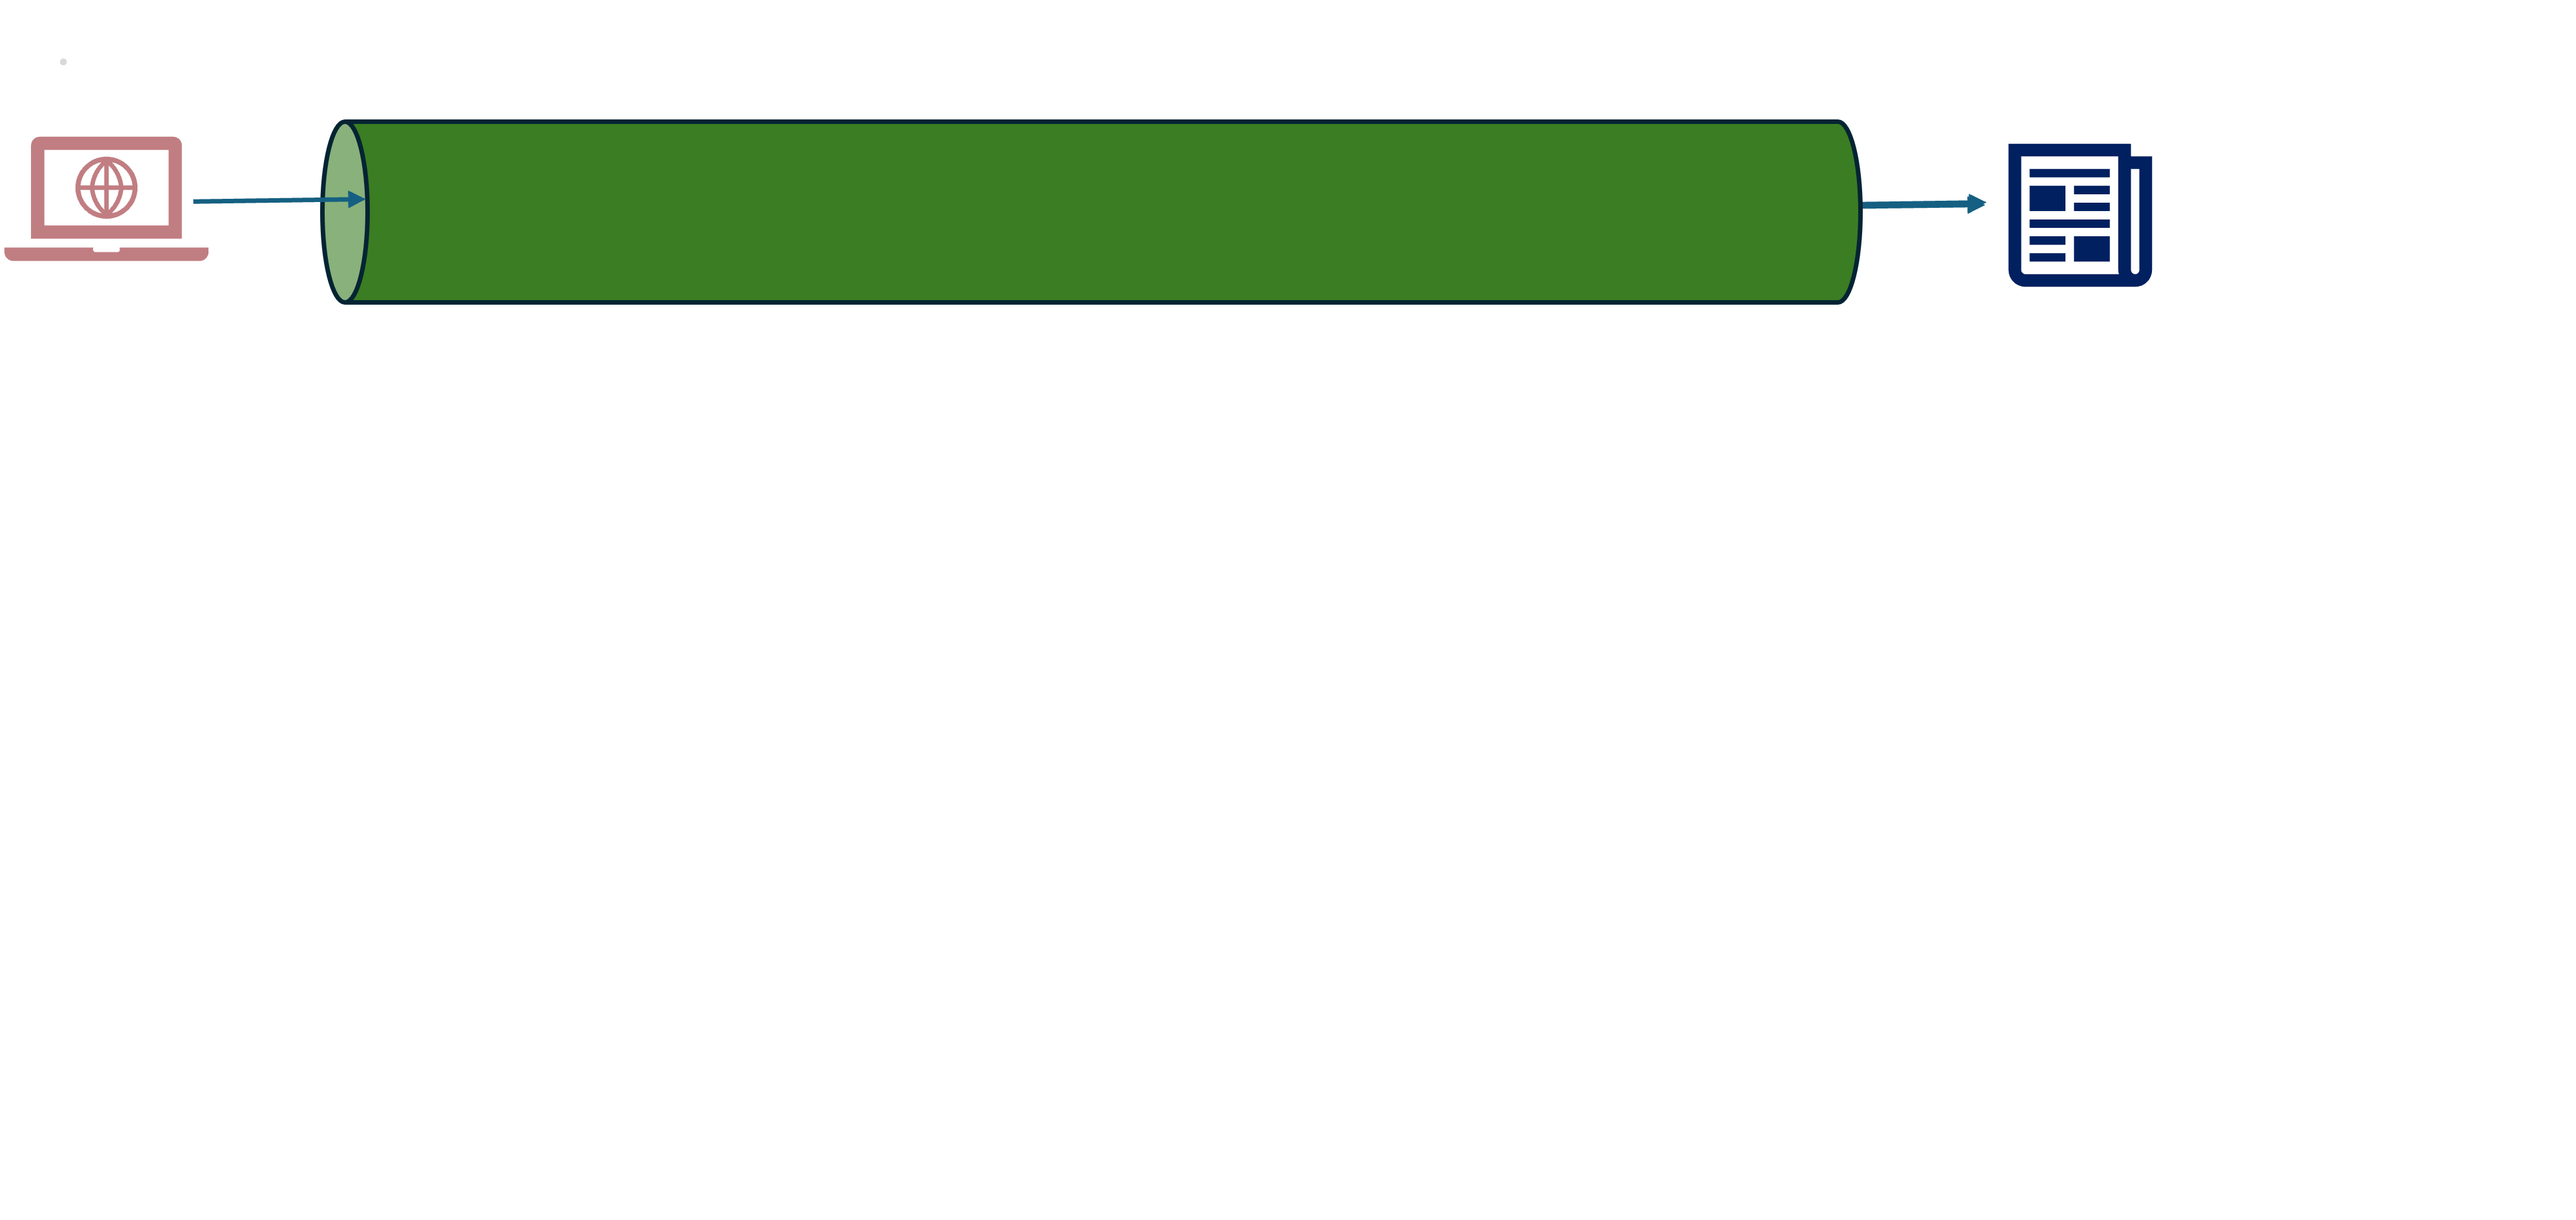
\includegraphics[width=0.8\textwidth]{Pipeline1.png} \\ Idealy, Input (website) and output (report) are linked}
        \only<2>{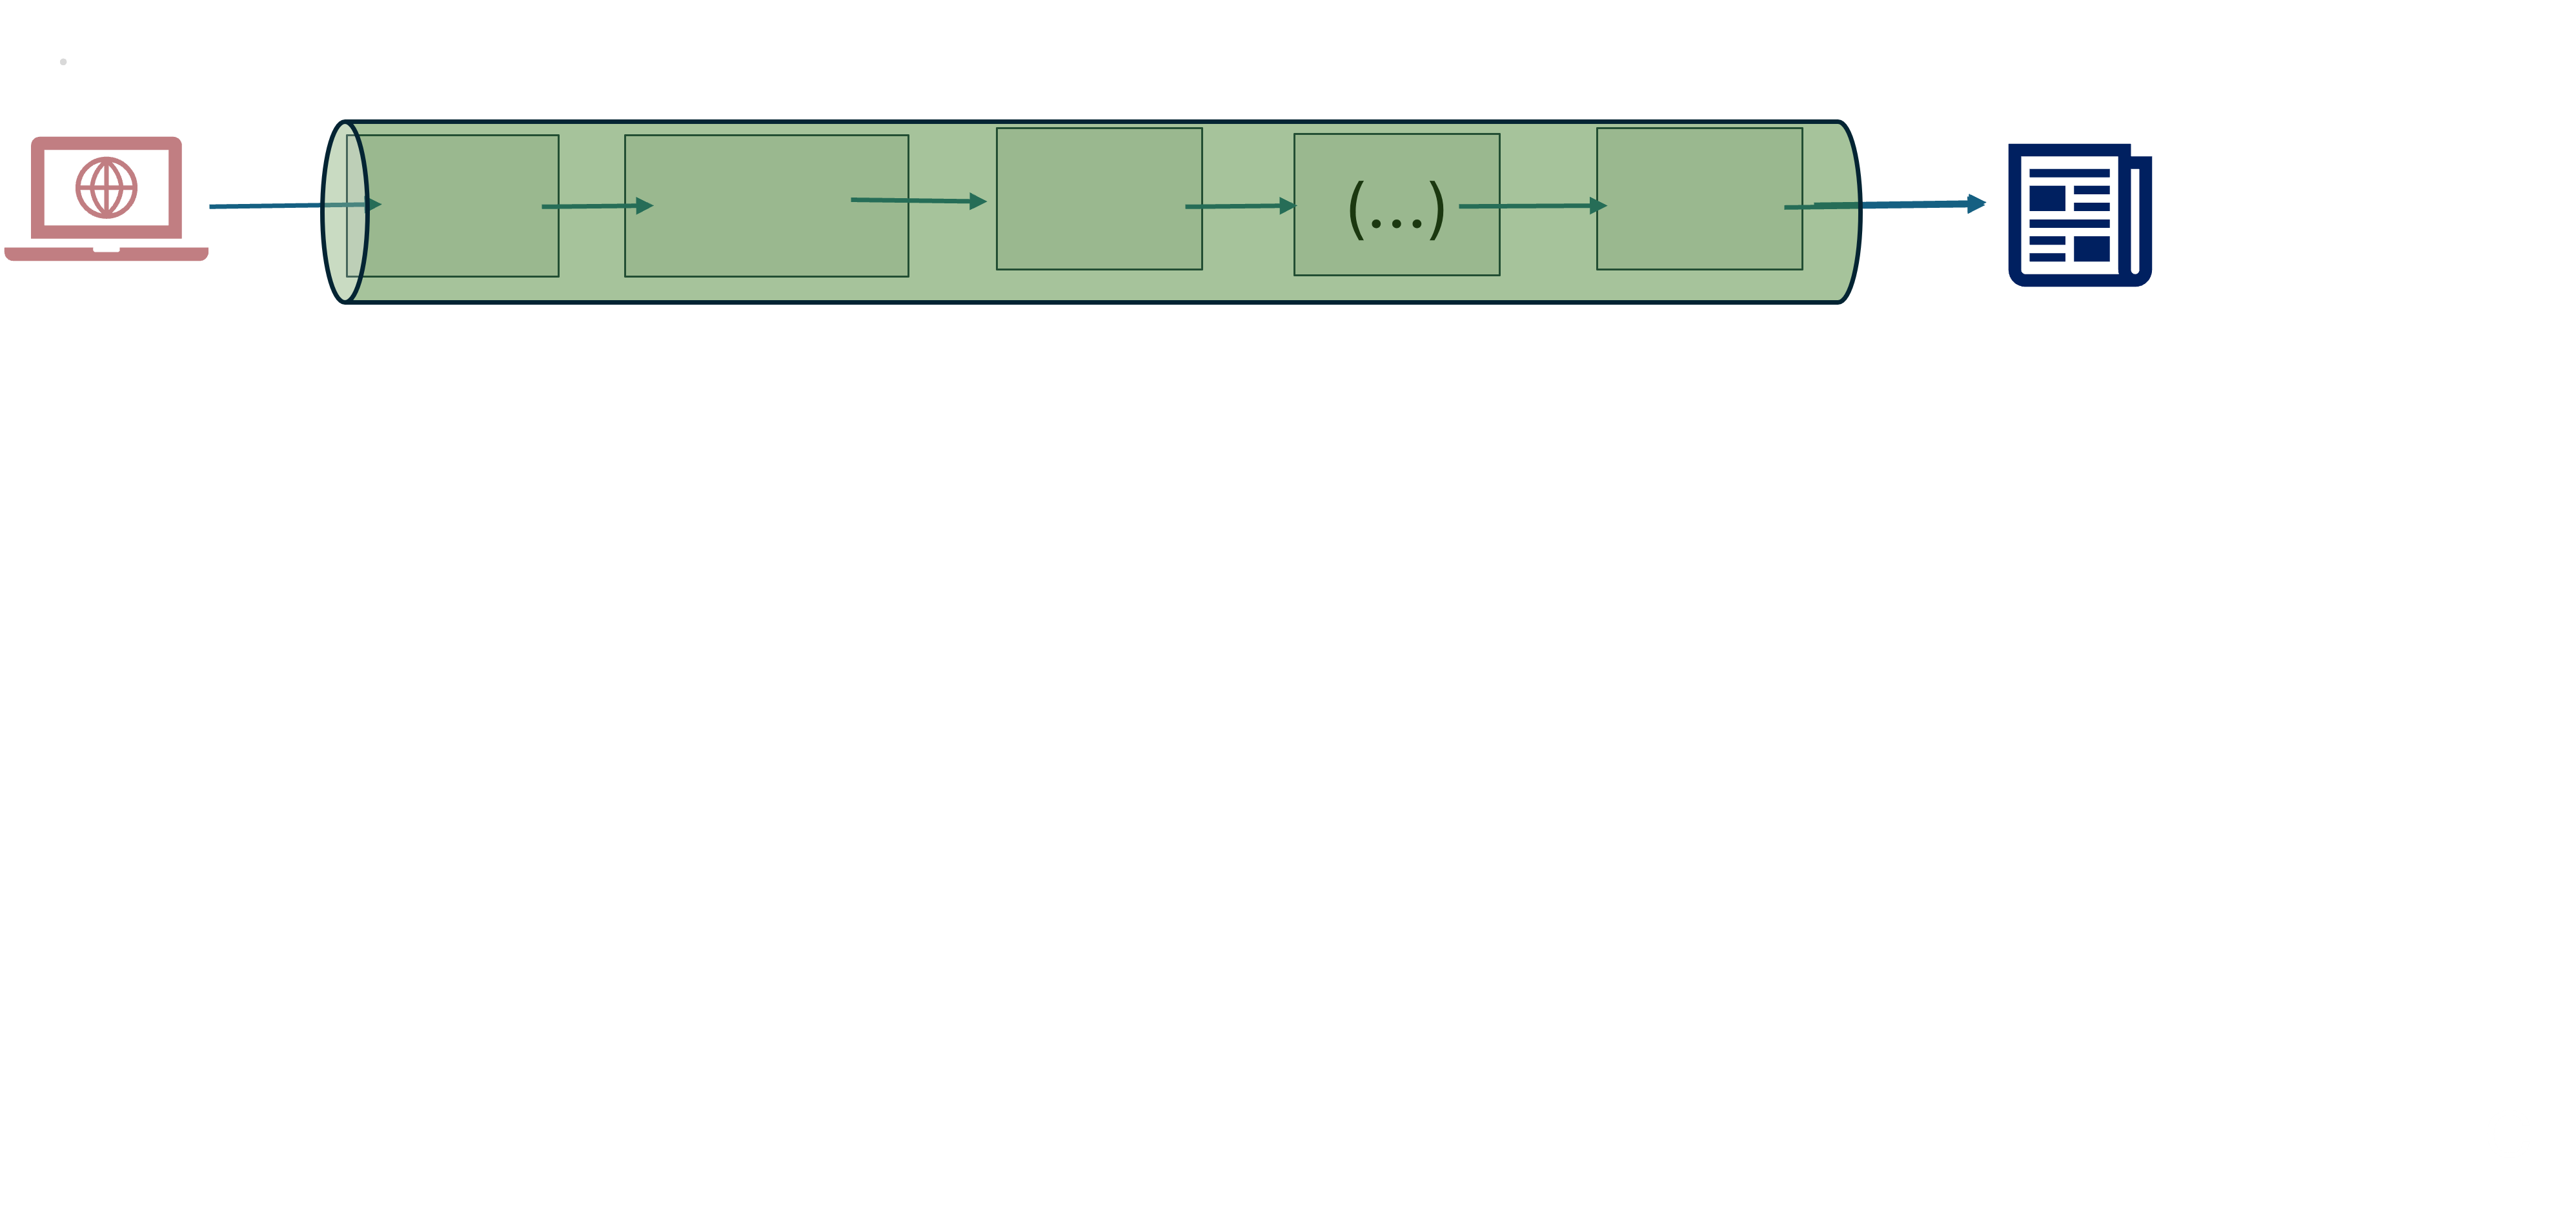
\includegraphics[width=0.8\textwidth]{Pipeline2.png} \\ Many steps are needed to create a report}
        \only<3>{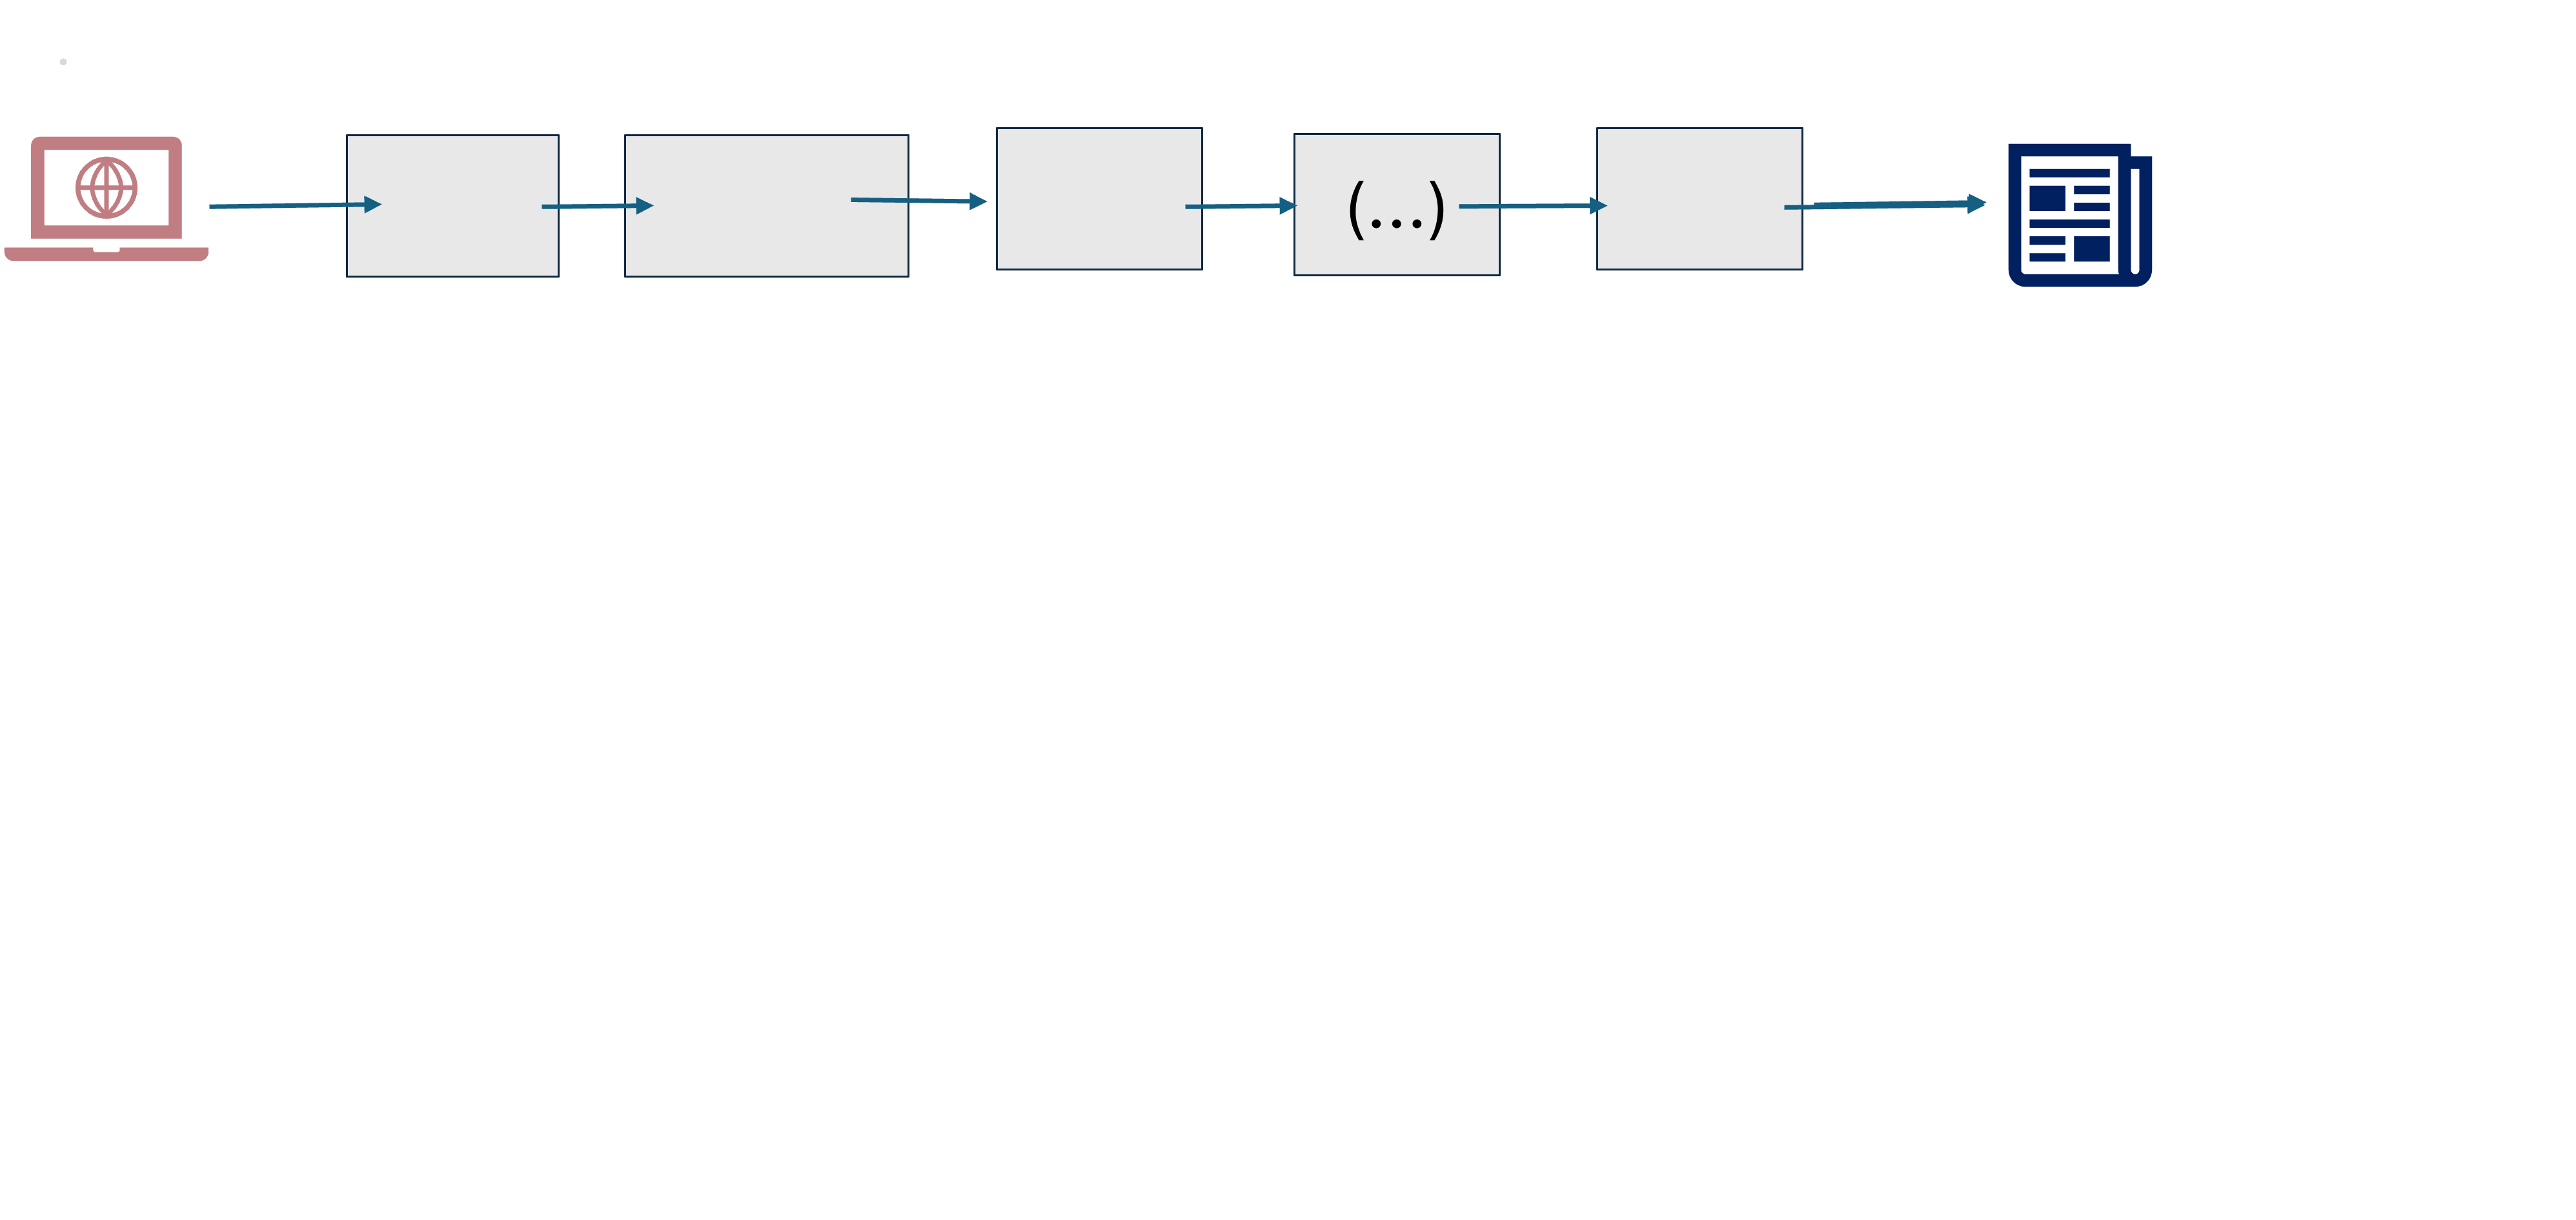
\includegraphics[width=0.8\textwidth]{Pipeline3.png} \\ All steps should be linked in a structured process}
        \only<4>{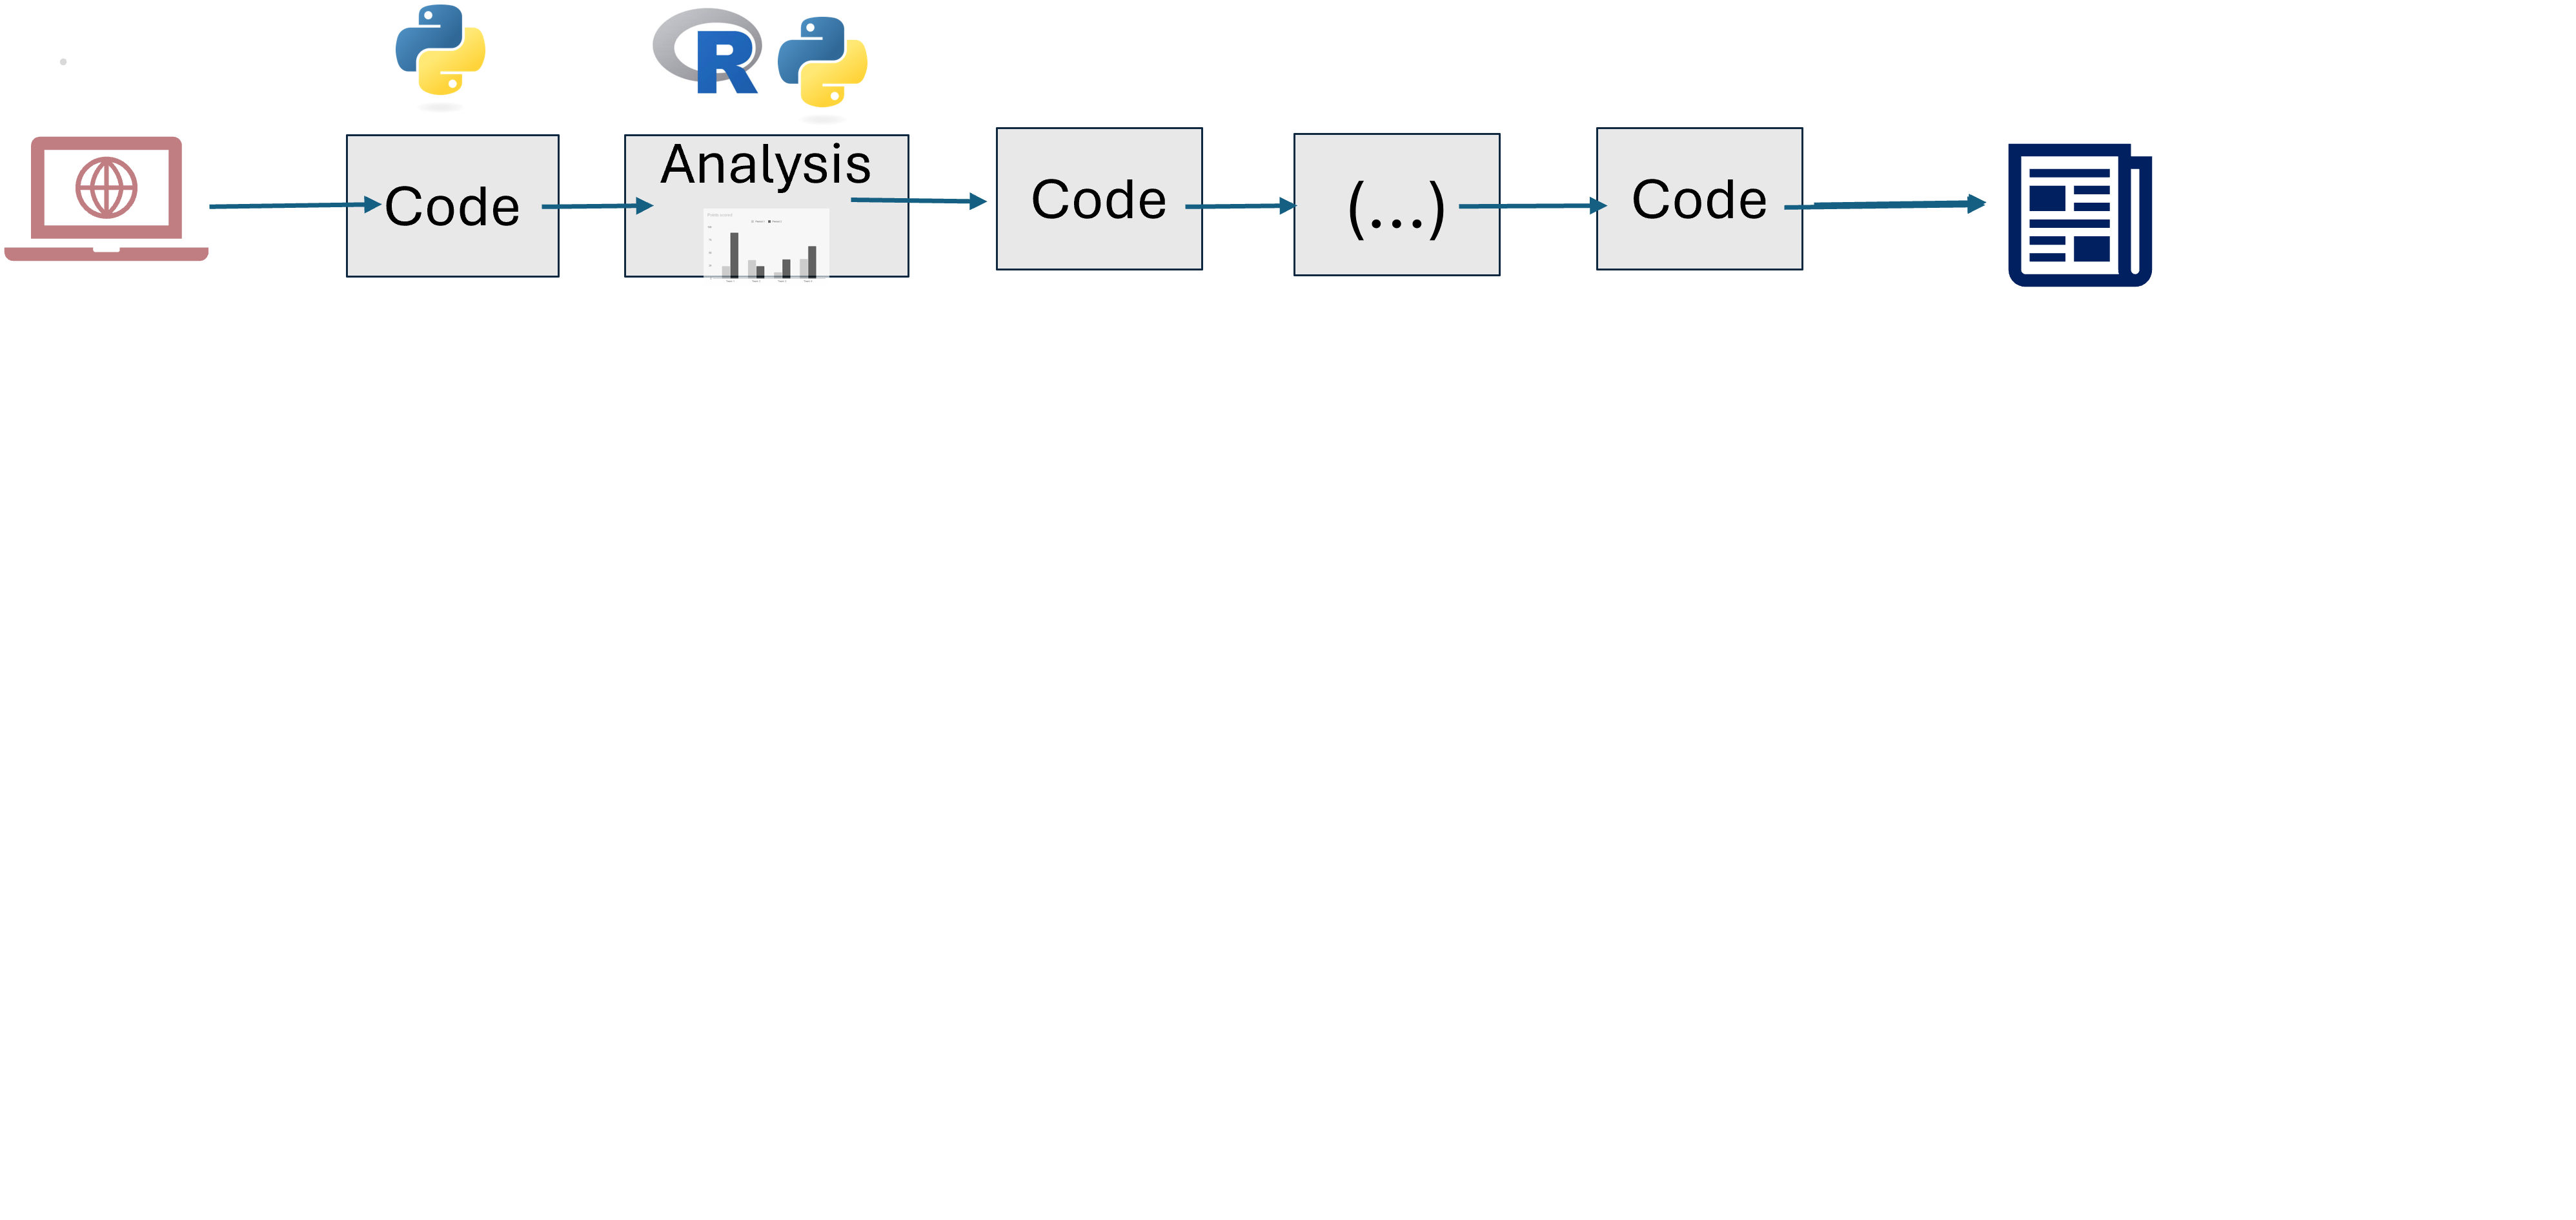
\includegraphics[width=0.8\textwidth]{Pipeline4.png} \\ And only through code (Python, R, \emph{Stata}), no copy/paste }
        \only<5>{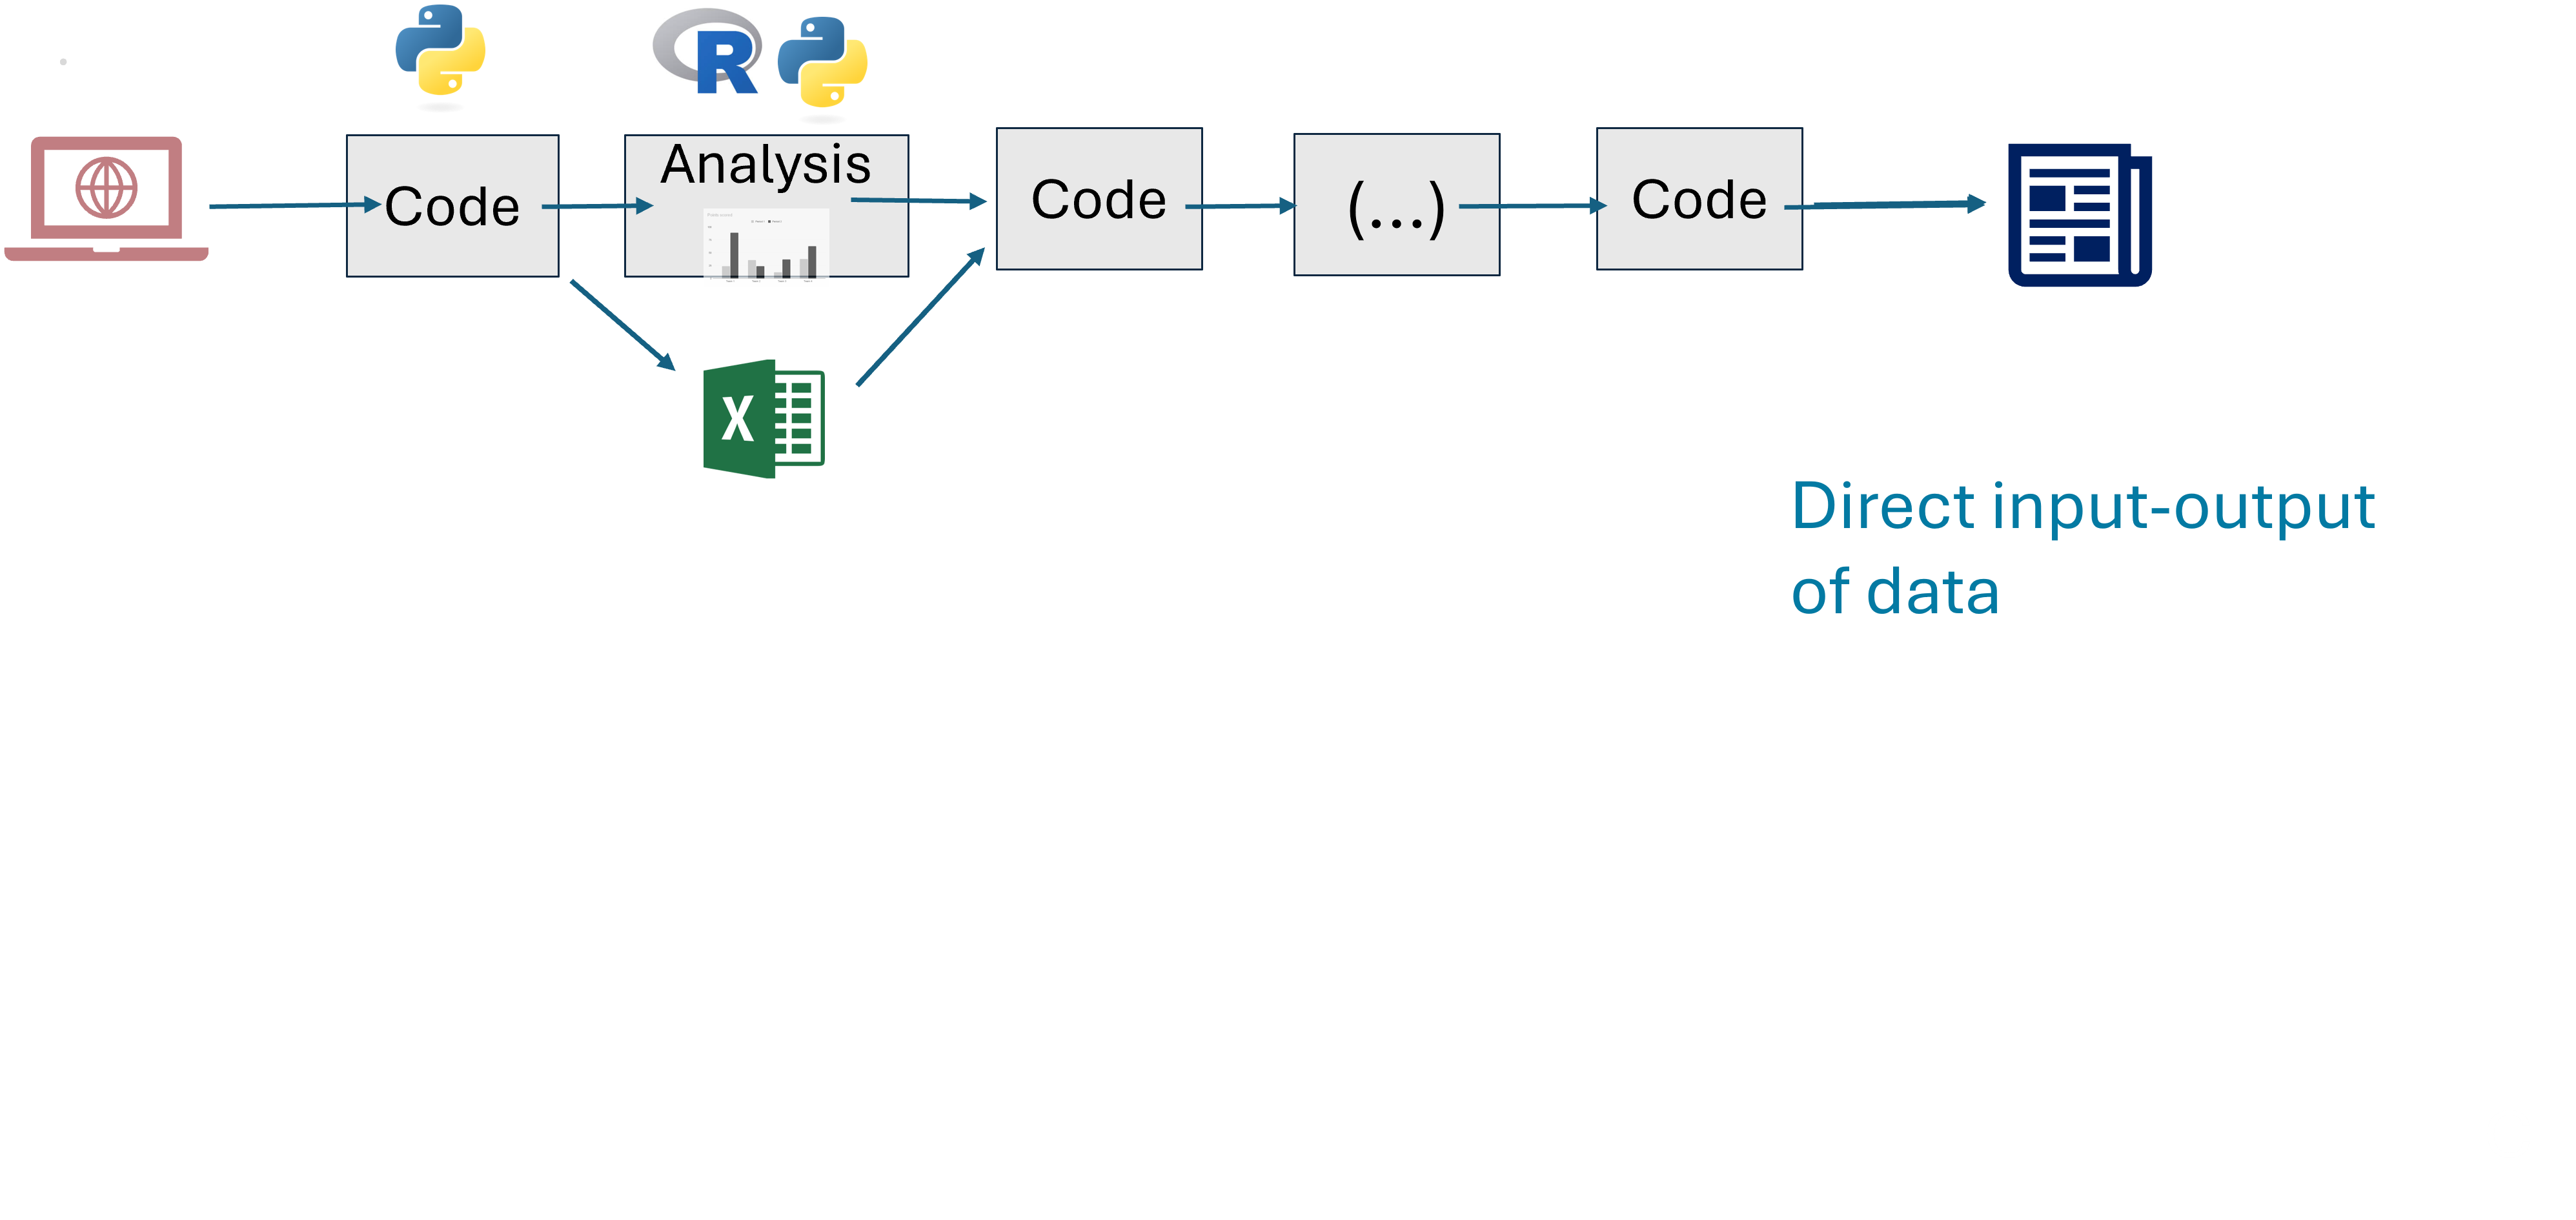
\includegraphics[width=0.8\textwidth]{Pipeline6.png} \\ There may be side-products, but with explicit output-input links}
        \only<6>{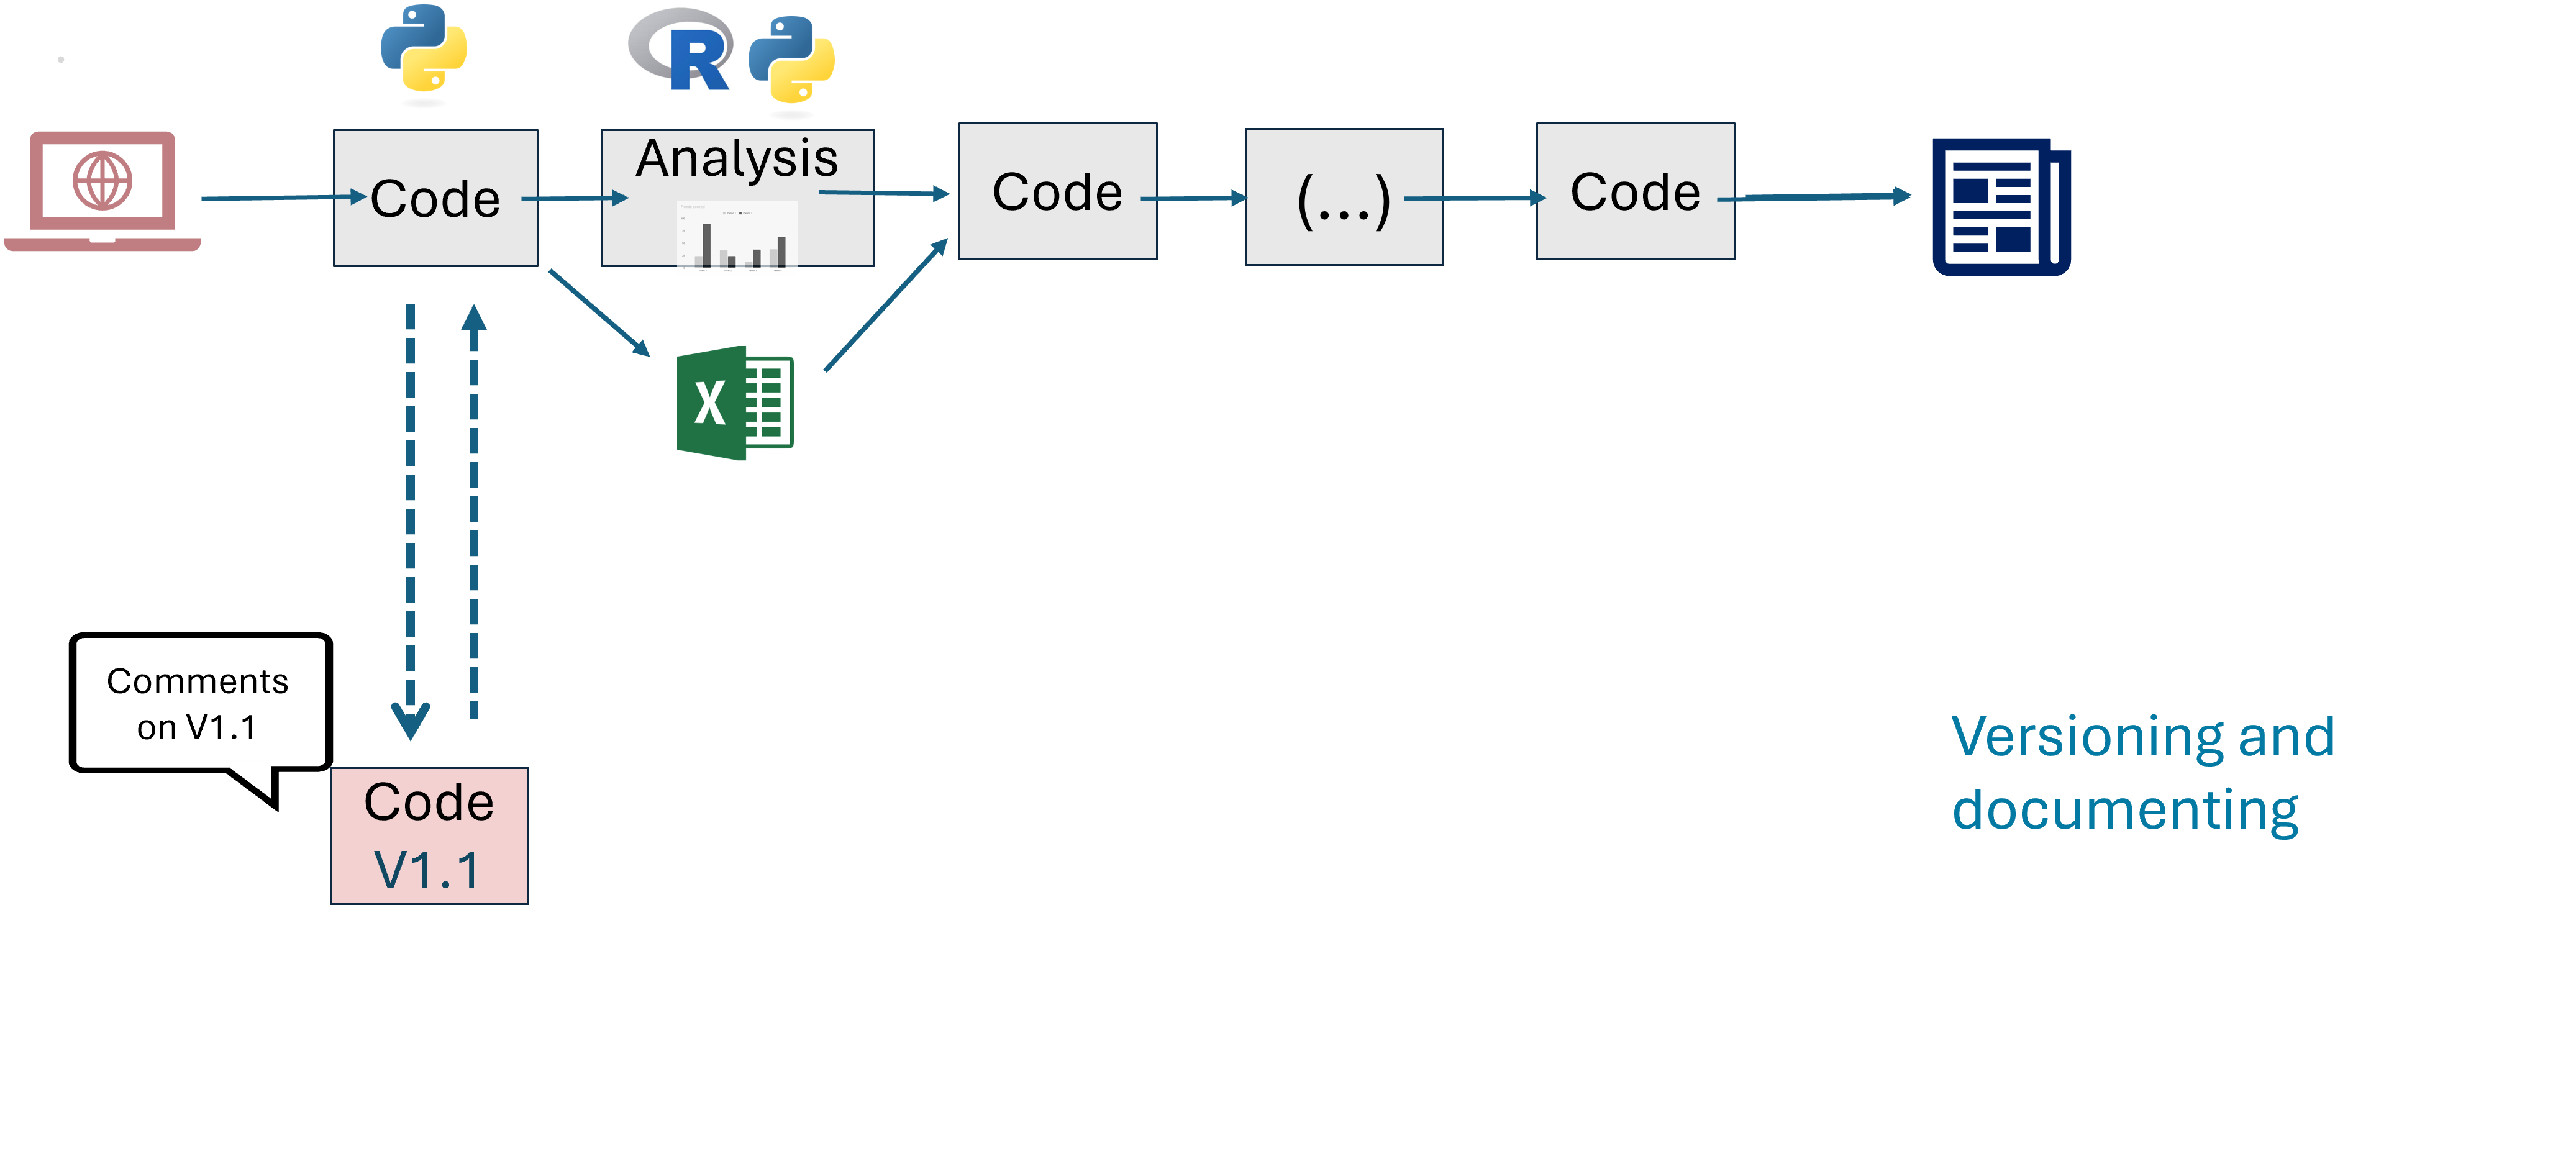
\includegraphics[width=0.8\textwidth]{Pipeline7.png} \\ If needed, code can be updated (new versions)}
        \only<7>{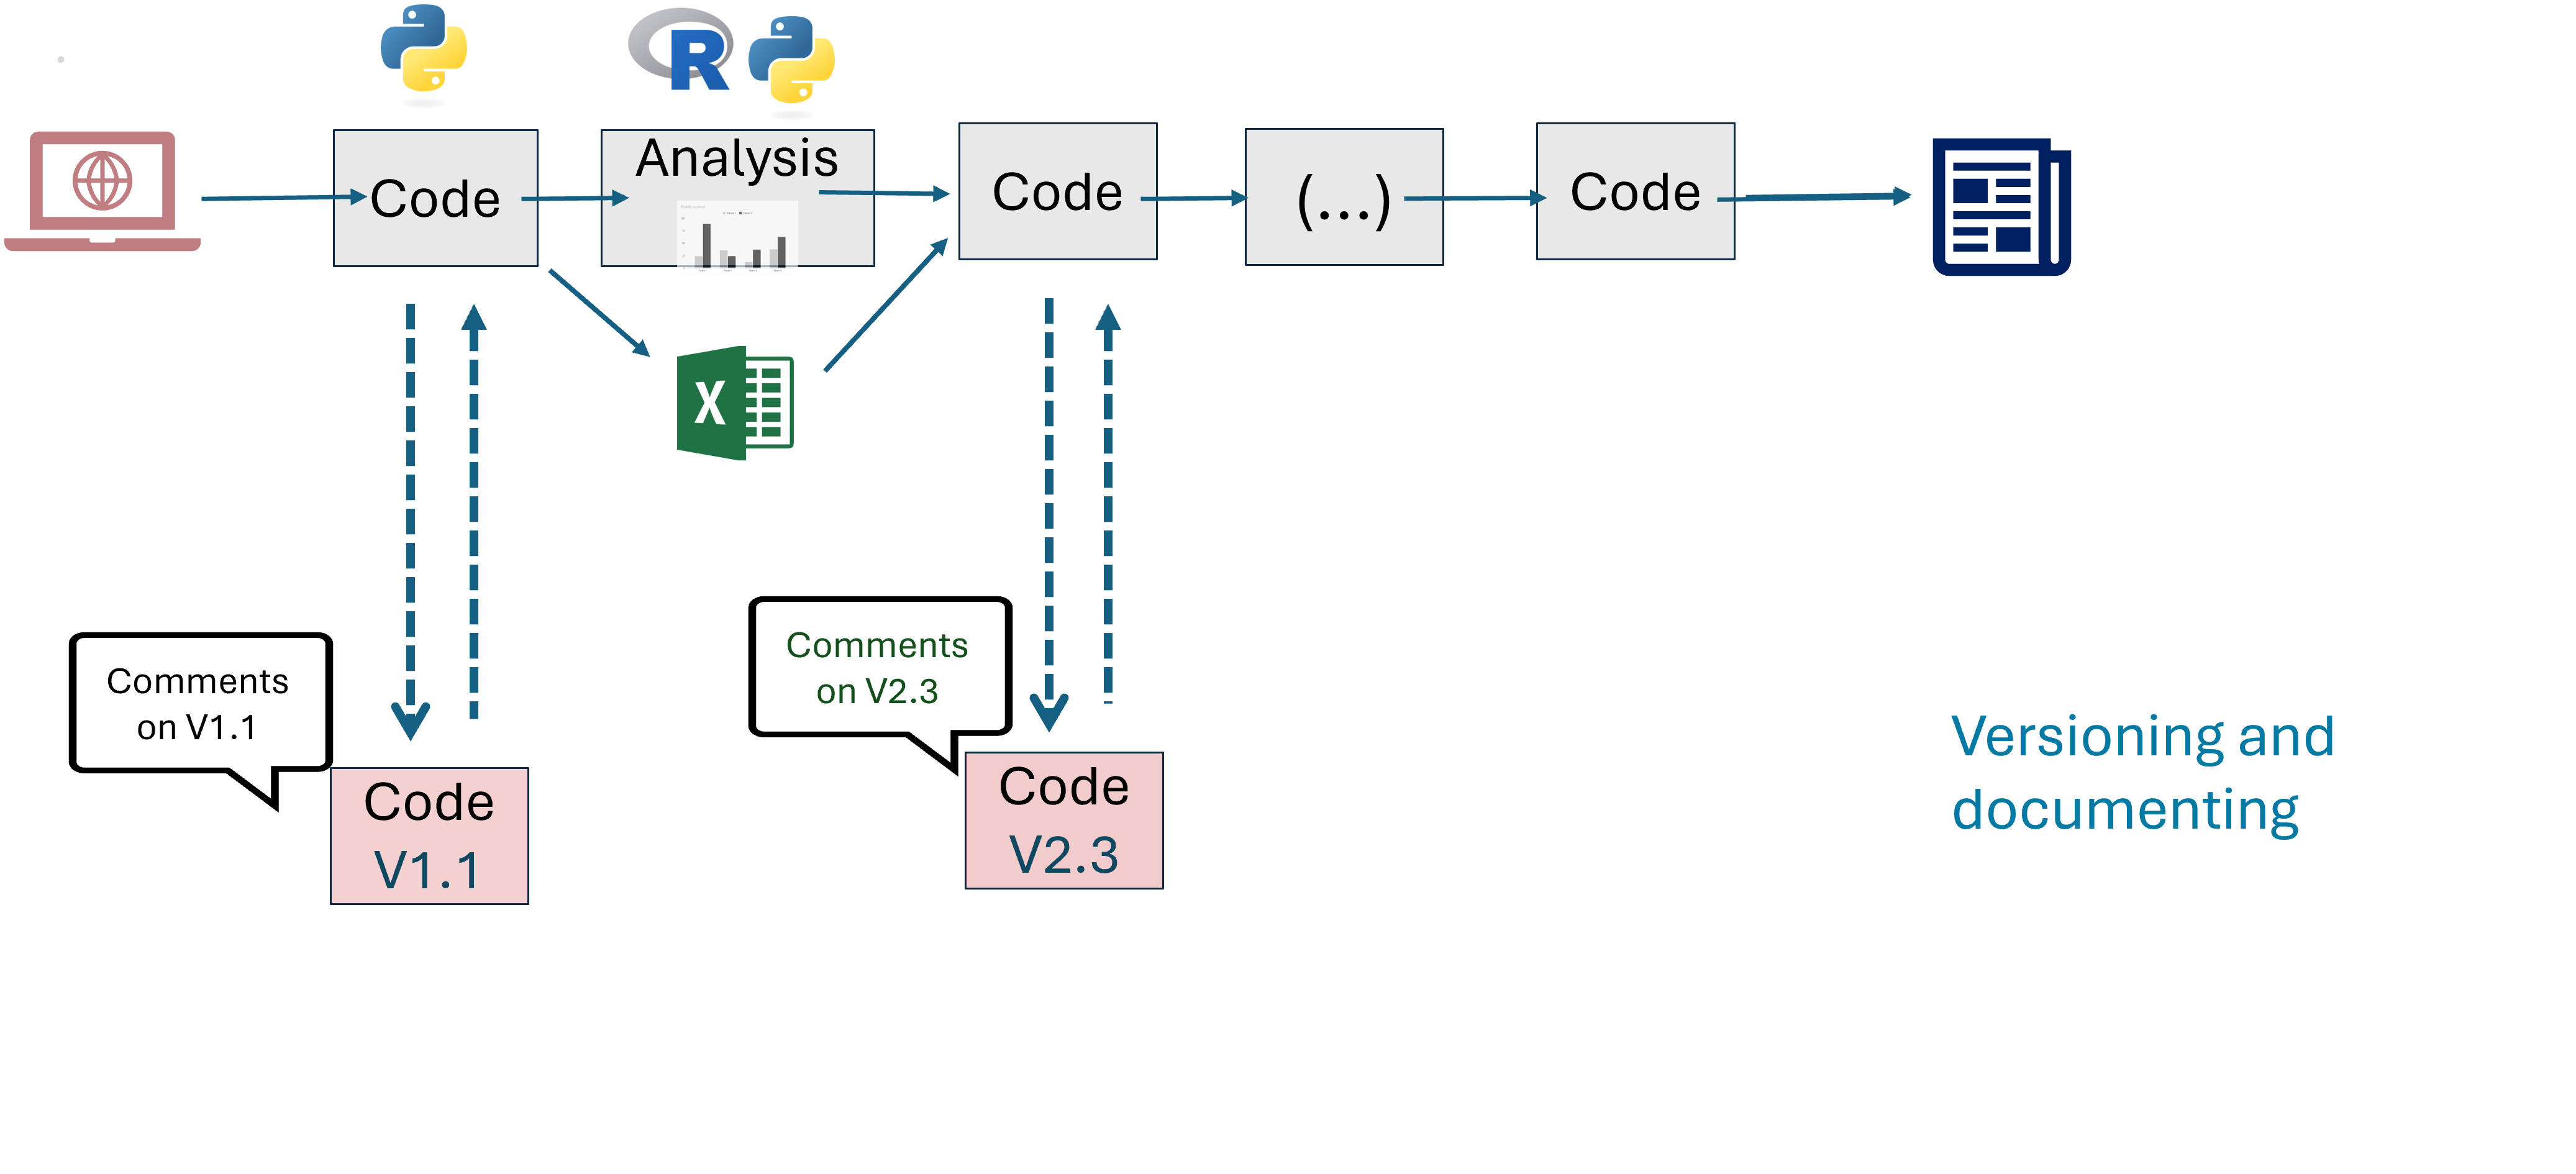
\includegraphics[width=0.8\textwidth]{Pipeline8.png} \\ And comments added for each change}
        \only<8>{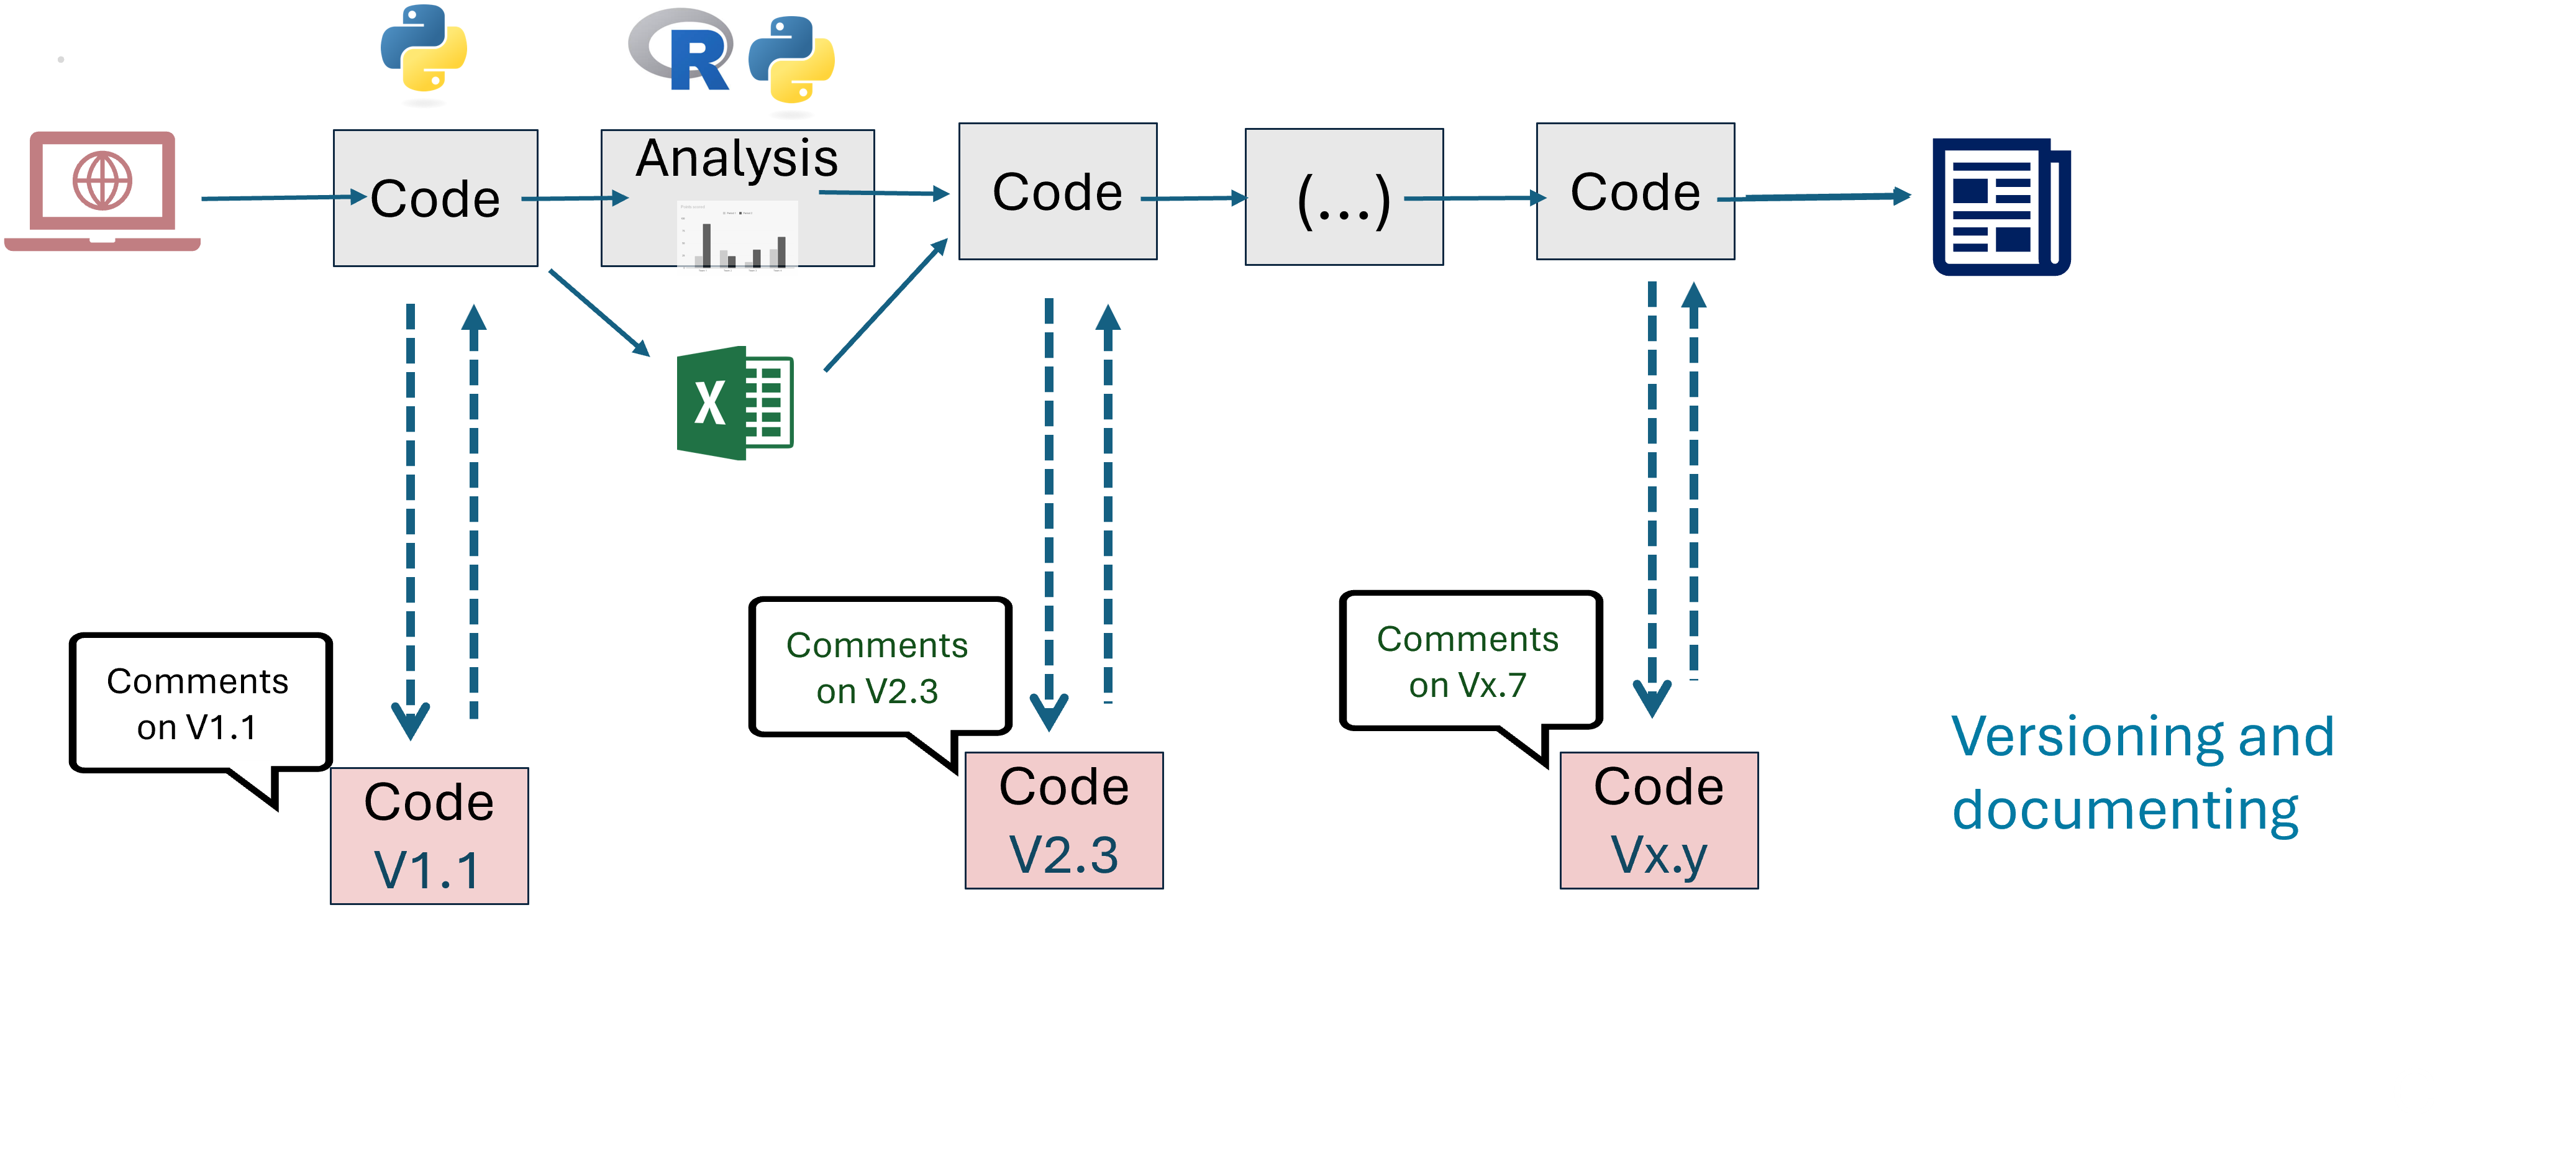
\includegraphics[width=0.8\textwidth]{Pipeline9.png} \\ Documentation on the process builds up with code changes}
        \only<9-10>{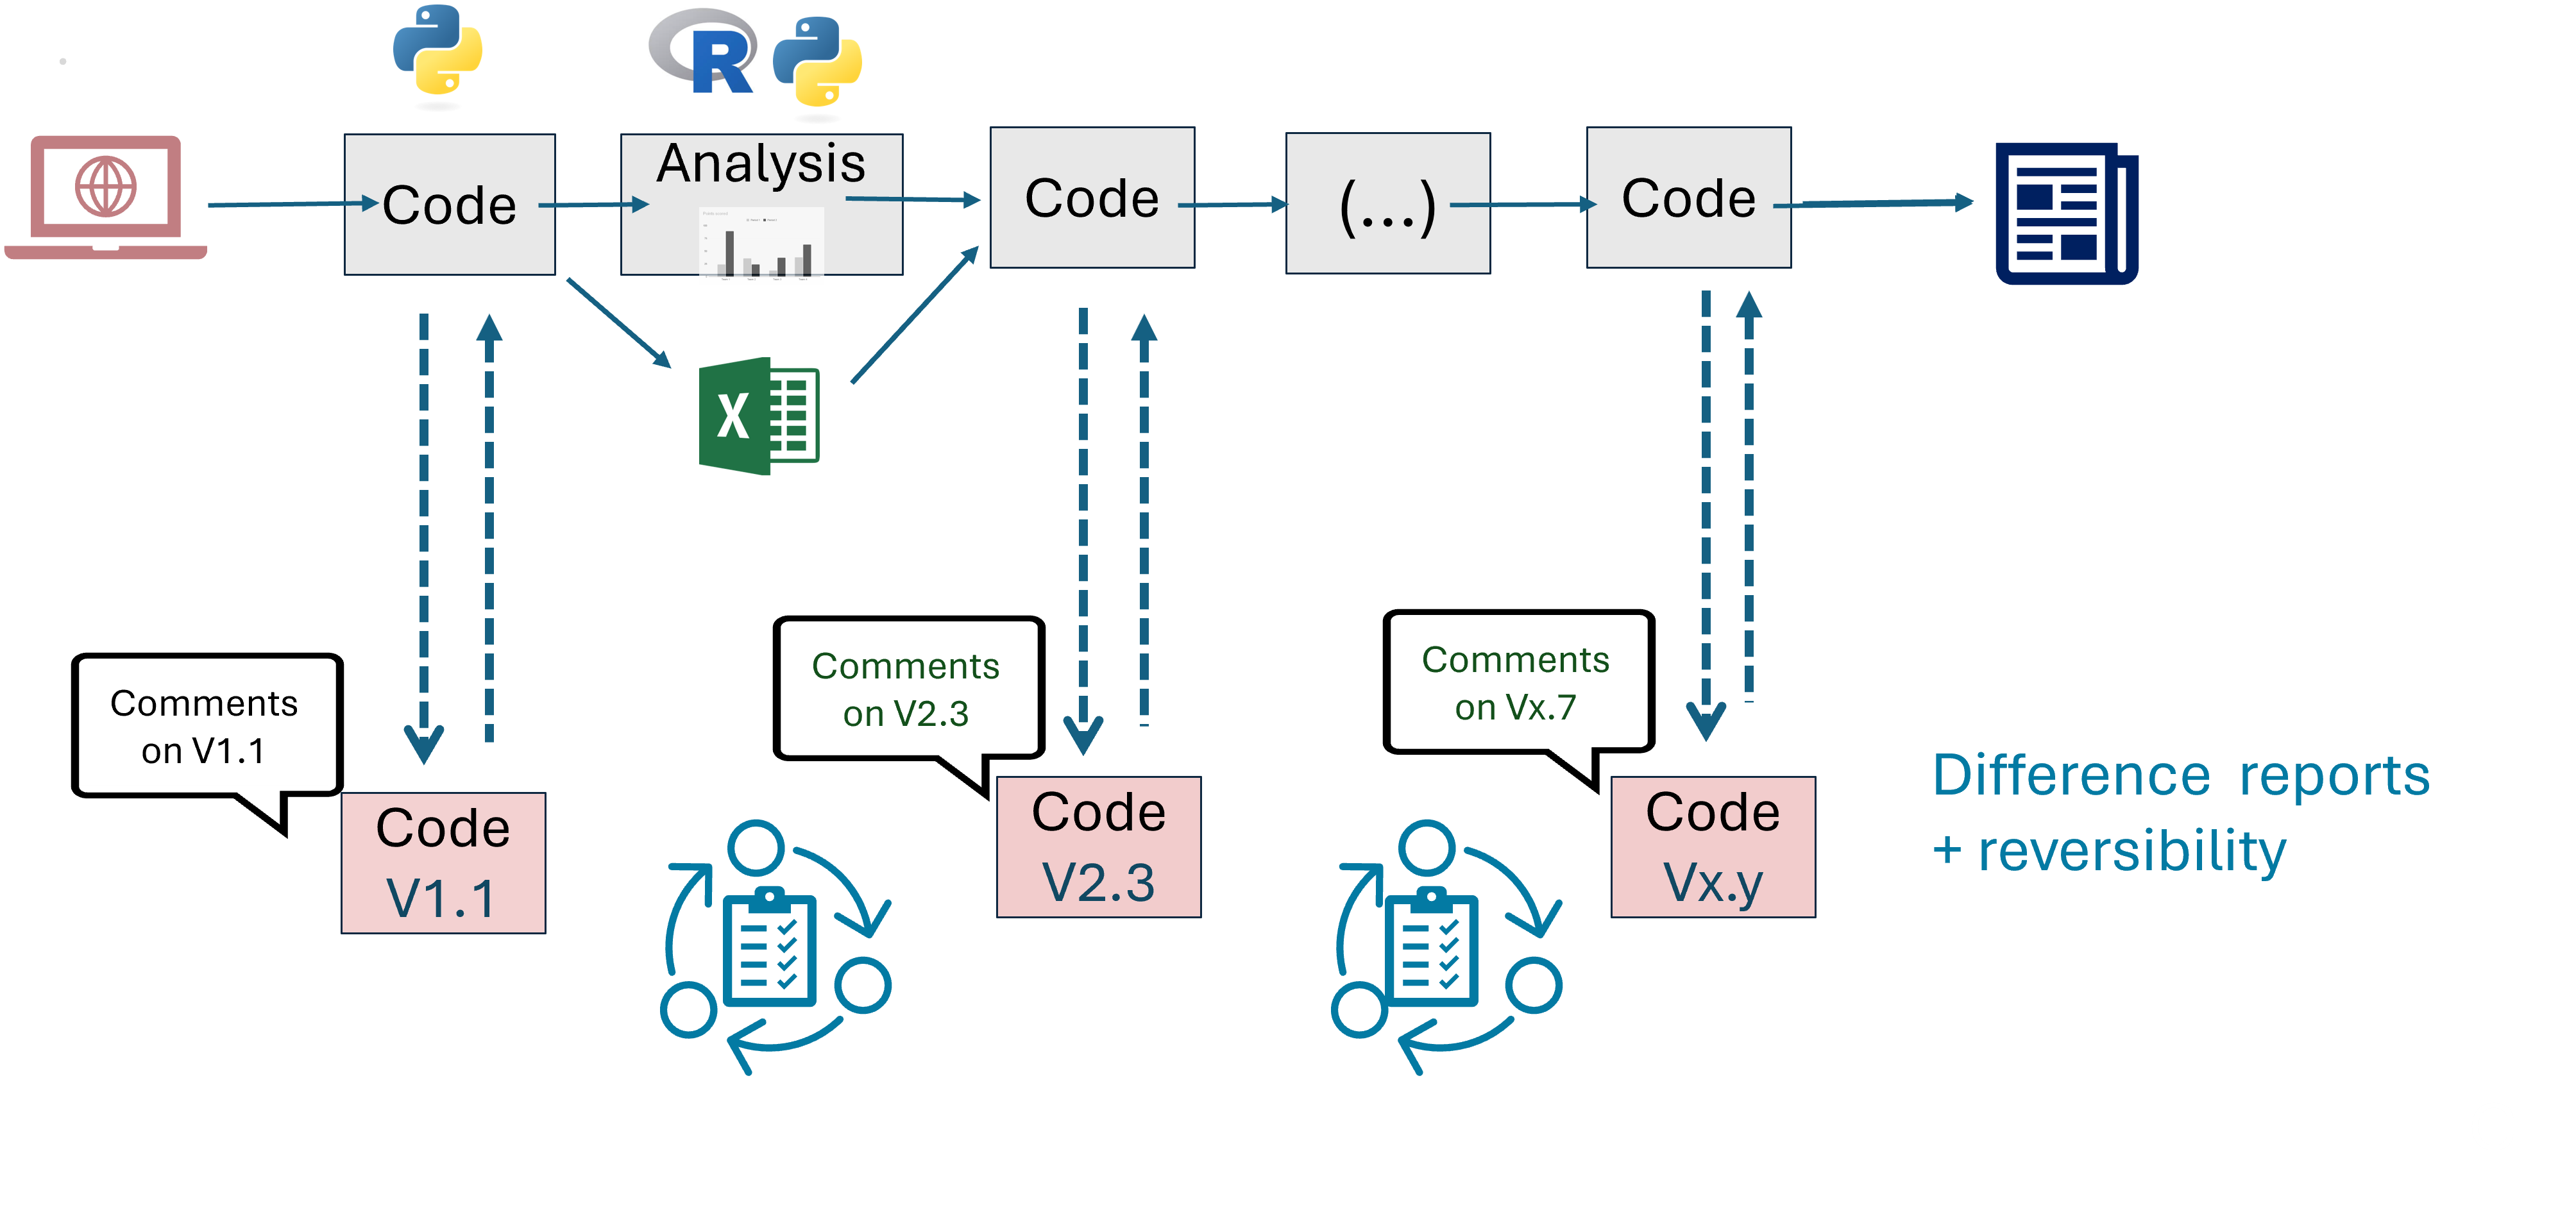
\includegraphics[width=0.8\textwidth]{Pipeline10.png} \\ }
        \only<10>{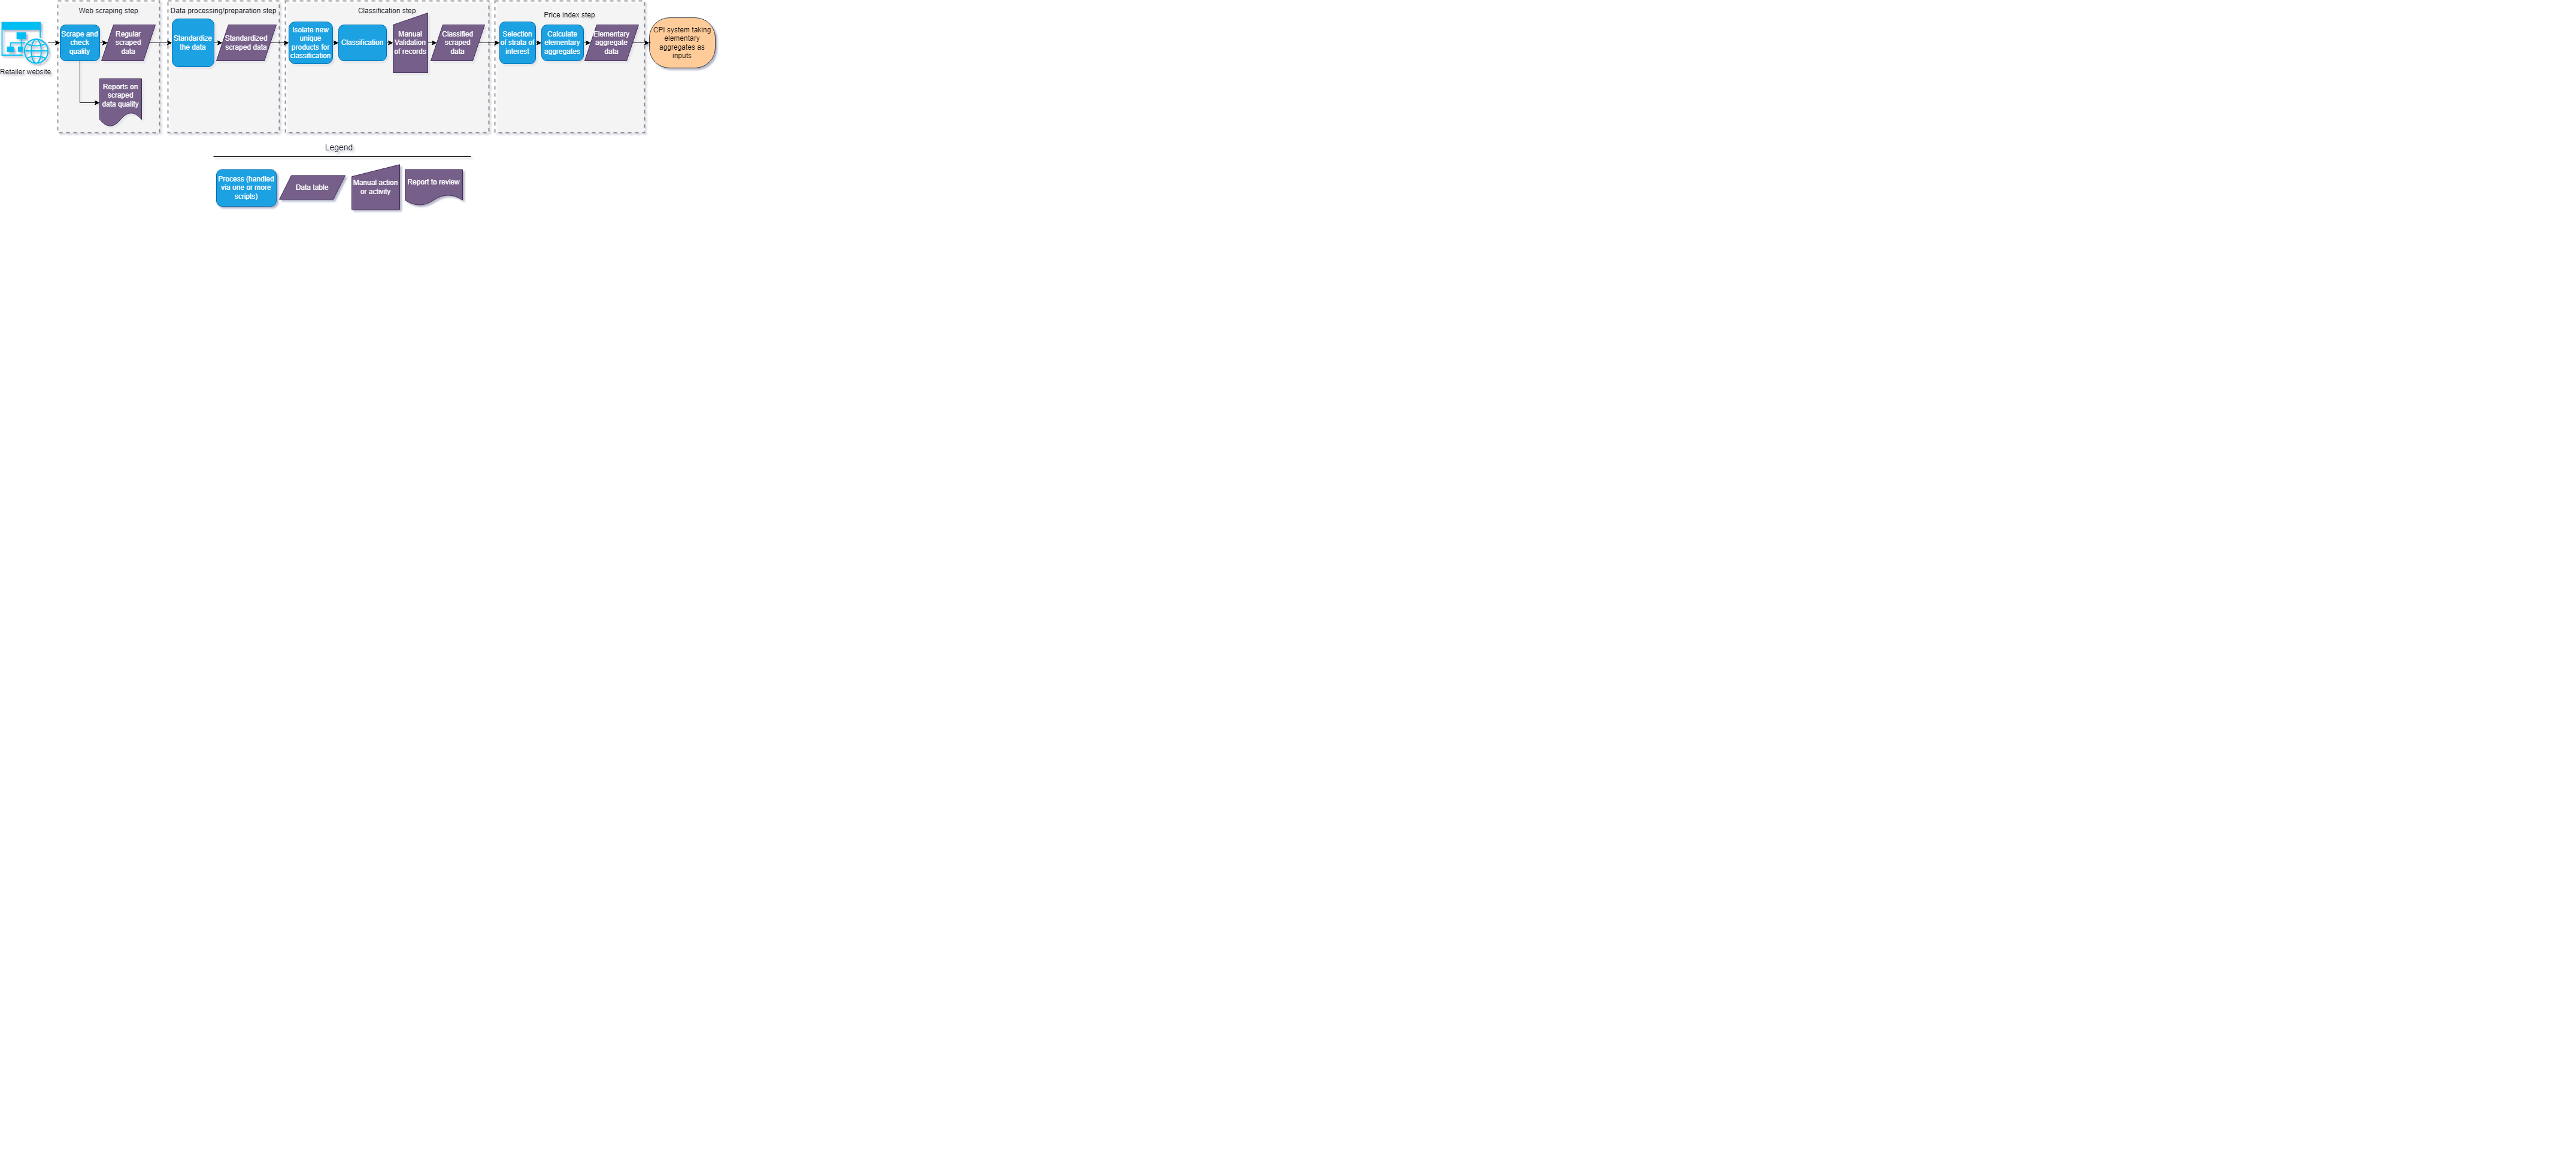
\includegraphics[width=0.8\textwidth]{ESCAPWebScrappingPipeline.png}}
        \only<11>{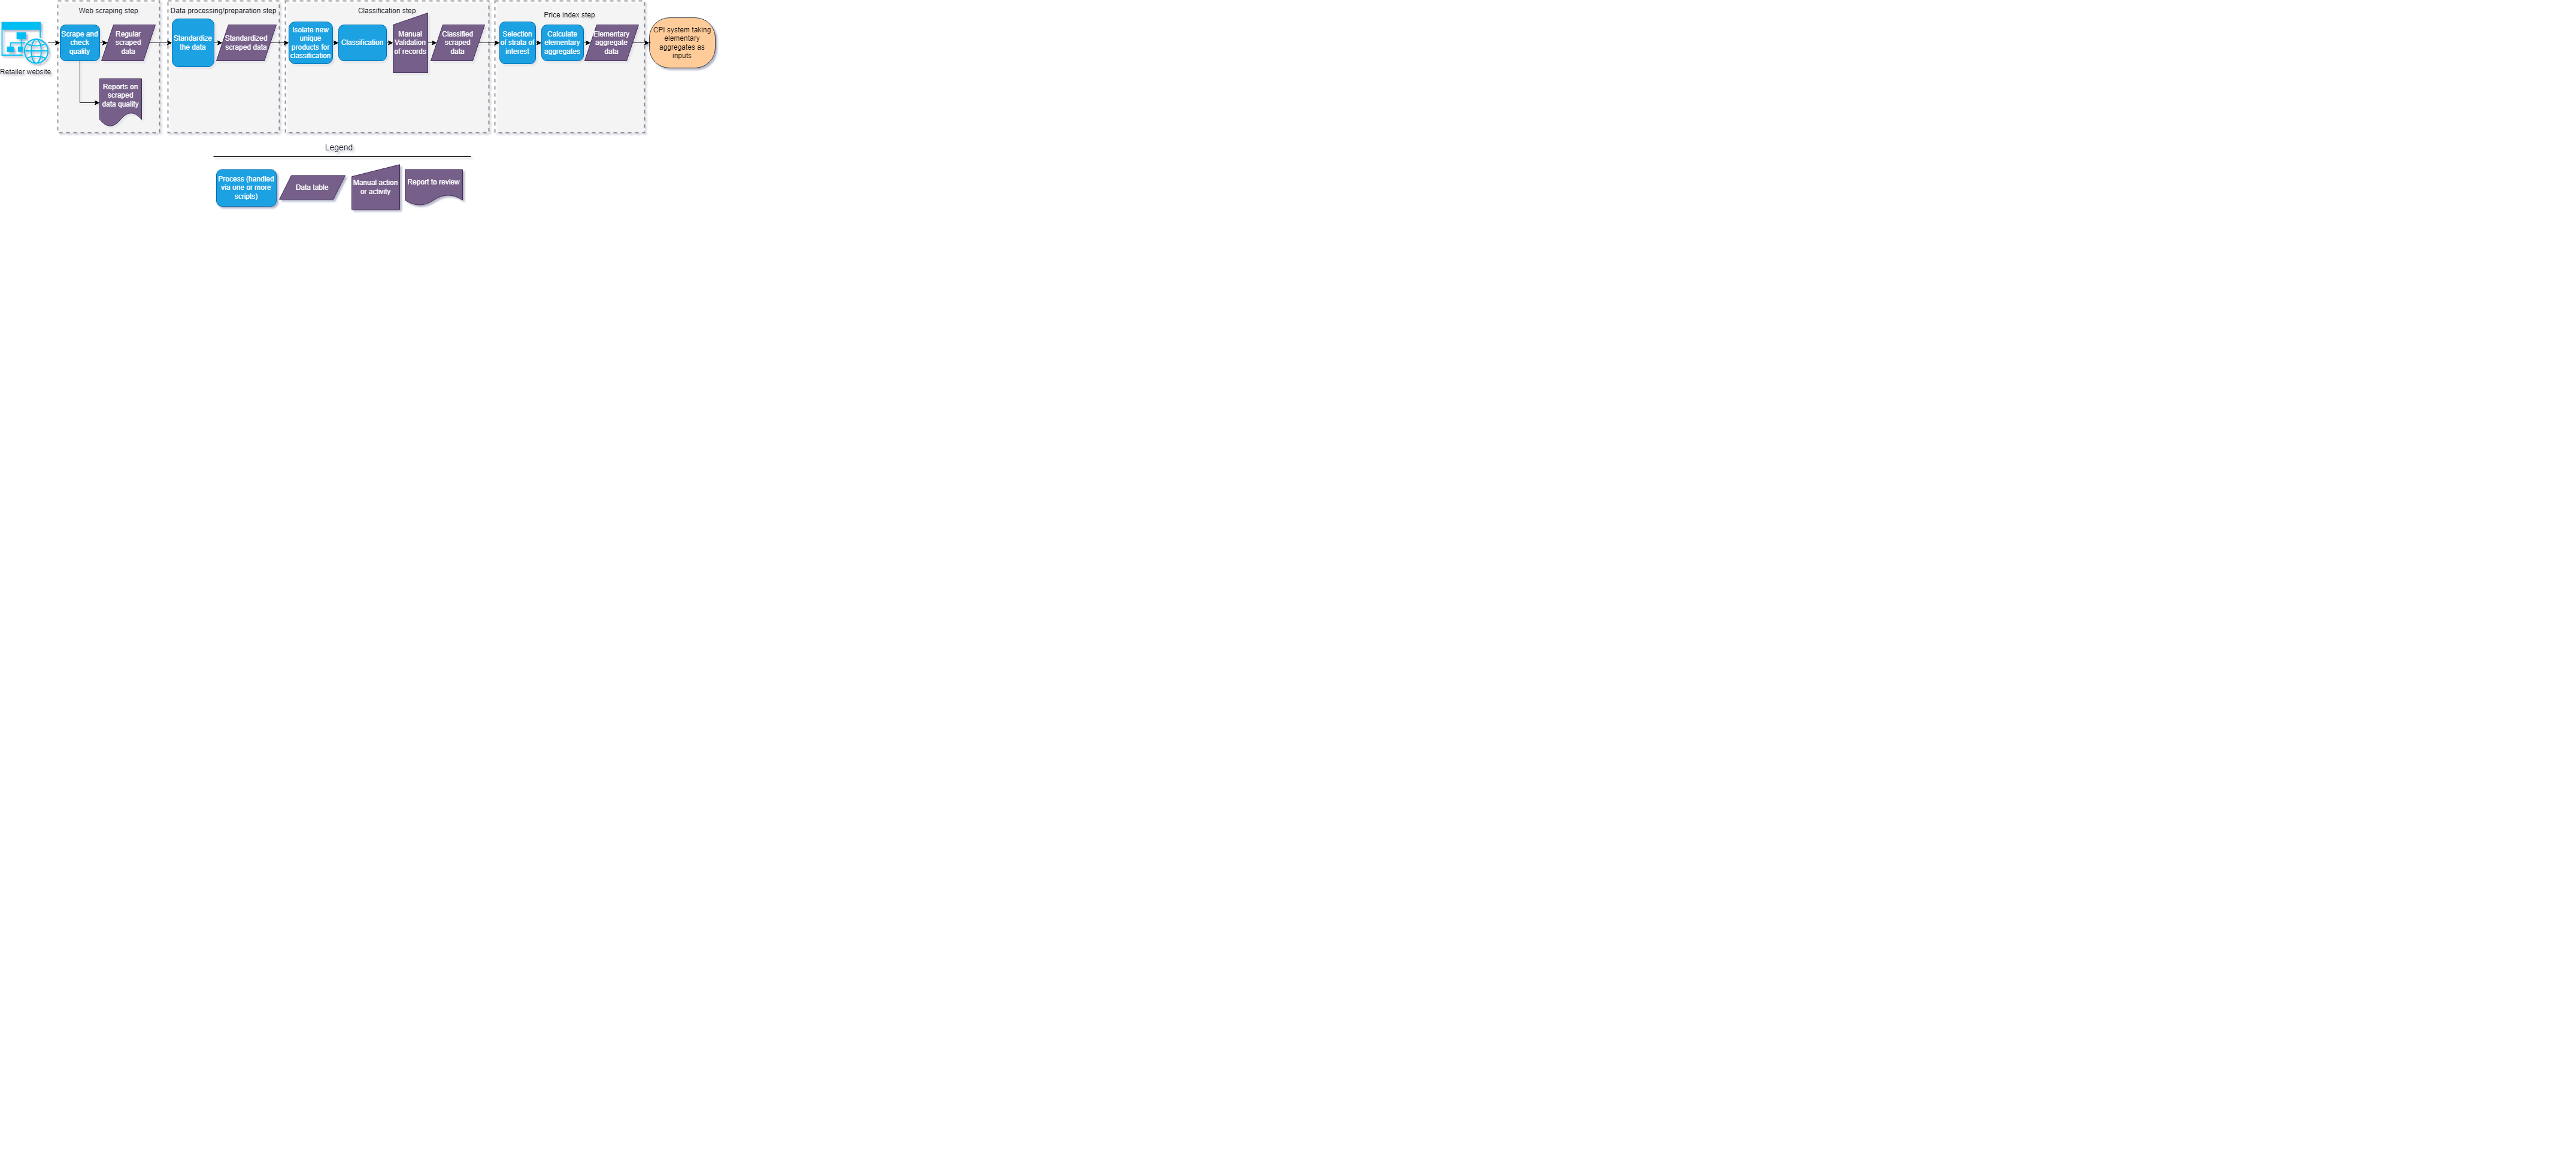
\includegraphics[width=1.0\textwidth]{ESCAPWebScrappingPipeline.png}}
    \end{itemize}
\end{center}
\end{frame}

\section{Principles- part 1}

\begin{frame}[<+->]
   \frametitle{RAP principles 1:\\  Automation - Modular coding}
   \pause
    \begin{itemize}[<+->]
     \item Automation (\emph{as much as you can})
     \item[$\hookrightarrow$]\href{https://sergegoussev.github.io/ESCAP_RAP_class/docs/applying_rap/process-mapping.html\#overview-of-the-ads-processing-view}{Where would you start? }
     \item[Tools:]\href{https://app.diagrams.net/}{Draw.io}, \href{https://www.figma.com/design/}{Figma}, $\cdots$
     \item Reusable (modular) code
     \item[$\hookrightarrow$]\href{https://sergegoussev.github.io/ESCAP_RAP_class/docs/teaching_materials/sept_18/sept_18_session.html\#principle-2-modular-re-usableBuild blocs}{What does this means for your project?}
     \item[$\hookrightarrow$]\href{https://sergegoussev.github.io/ESCAP_RAP_class/docs/teaching_materials/sept_18/sept_18_session.html\#what-does-this-mean-if-we-put-it-together}{Example}
     \item \href{https://sergegoussev.github.io/ESCAP_RAP_class/docs/teaching_materials/sept_18/sept_18_session.html\#excercize-1}{\emph{Exercise part 1}} (15 minutes)
     \item[-] \emph{Look at a notebook that you developed for this course - and see how to separate out what you did into functions.}
     \item[-] \href{https://nhsdigital.github.io/rap-community-of-practice/training_resources/python/python-functions/\#coding-challenge}{\emph{Create functions, use these functions in a main document}}
    \end{itemize}
\end{frame}


\section{Principles- part 2}

\begin{frame}[<+->]
   \frametitle{RAP principles 2:  \\Transparency - open source - version control }
   \pause
    \begin{itemize}[<+->]
      \item Transparency
     \item[$\hookrightarrow$]\href{https://sergegoussev.github.io/ESCAP_RAP_class/docs/teaching_materials/sept_18/sept_18_session.html\#principle-3-transparency}{What are the benefits of working in a transparent way? }
     \item Use open source tools
      \item[$\hookrightarrow$]\href{https://sergegoussev.github.io/ESCAP_RAP_class/docs/teaching_materials/sept_18/sept_18_session.html\#practical-set-two}{Compare Open source \emph{vs} proprietary software }
     \item[Tools:] Python, R, Git, GitHub(GitLab)
     \item Version control
     \item \href{https://sergegoussev.github.io/ESCAP_RAP_class/docs/teaching_materials/sept_18/sept_18_session.html\#excercize-1}{\emph{Exercise part 2}} (Afternoon session)
    \end{itemize}
\end{frame}

\section{Git principles}

\begin{frame}{Version Control Main commands}
\emph{commit} for every change!
\begin{center}
\begin{itemize}
   \only<1> {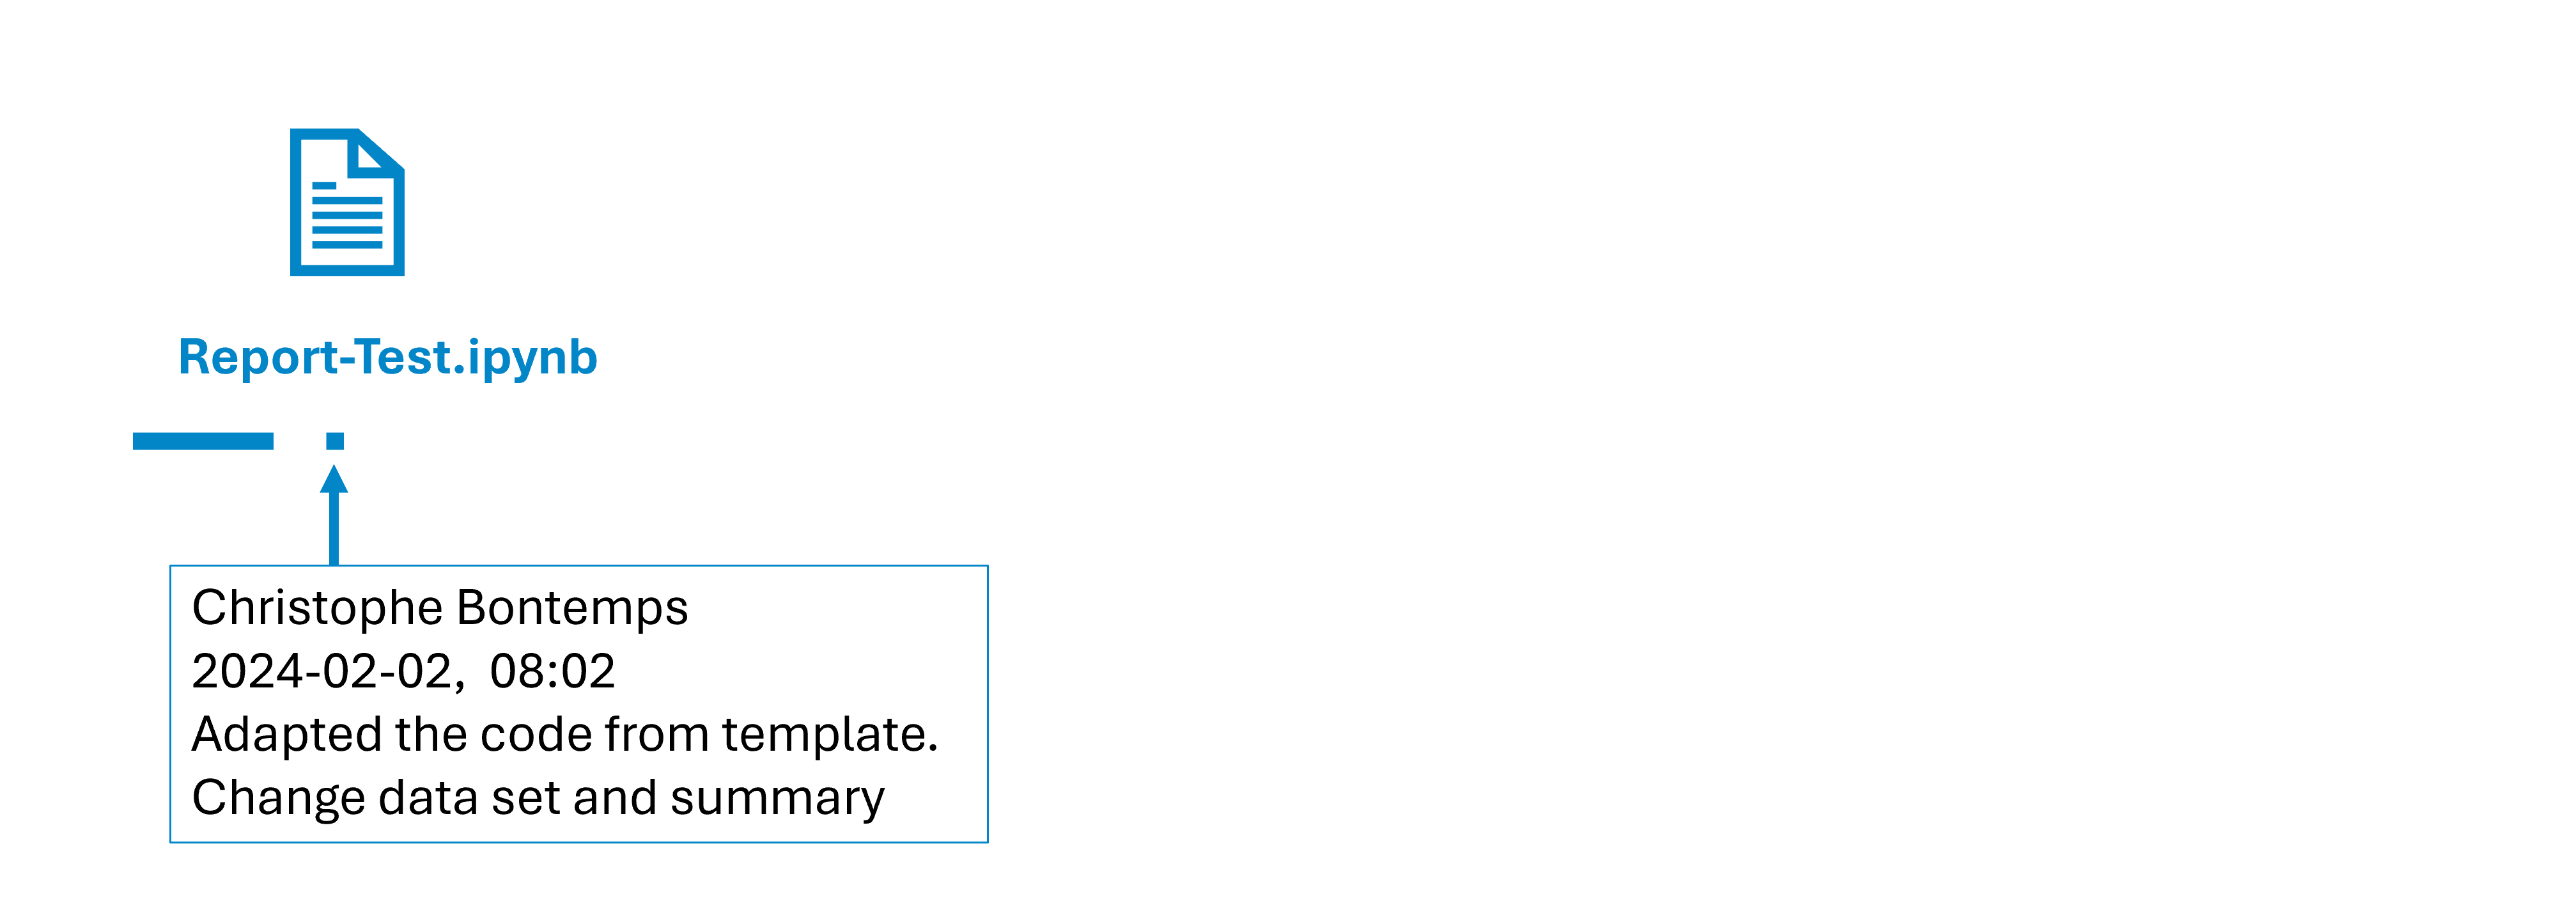
\includegraphics[width = 1.0\textwidth]{FileLife1.png} \\ }
   \only<2> {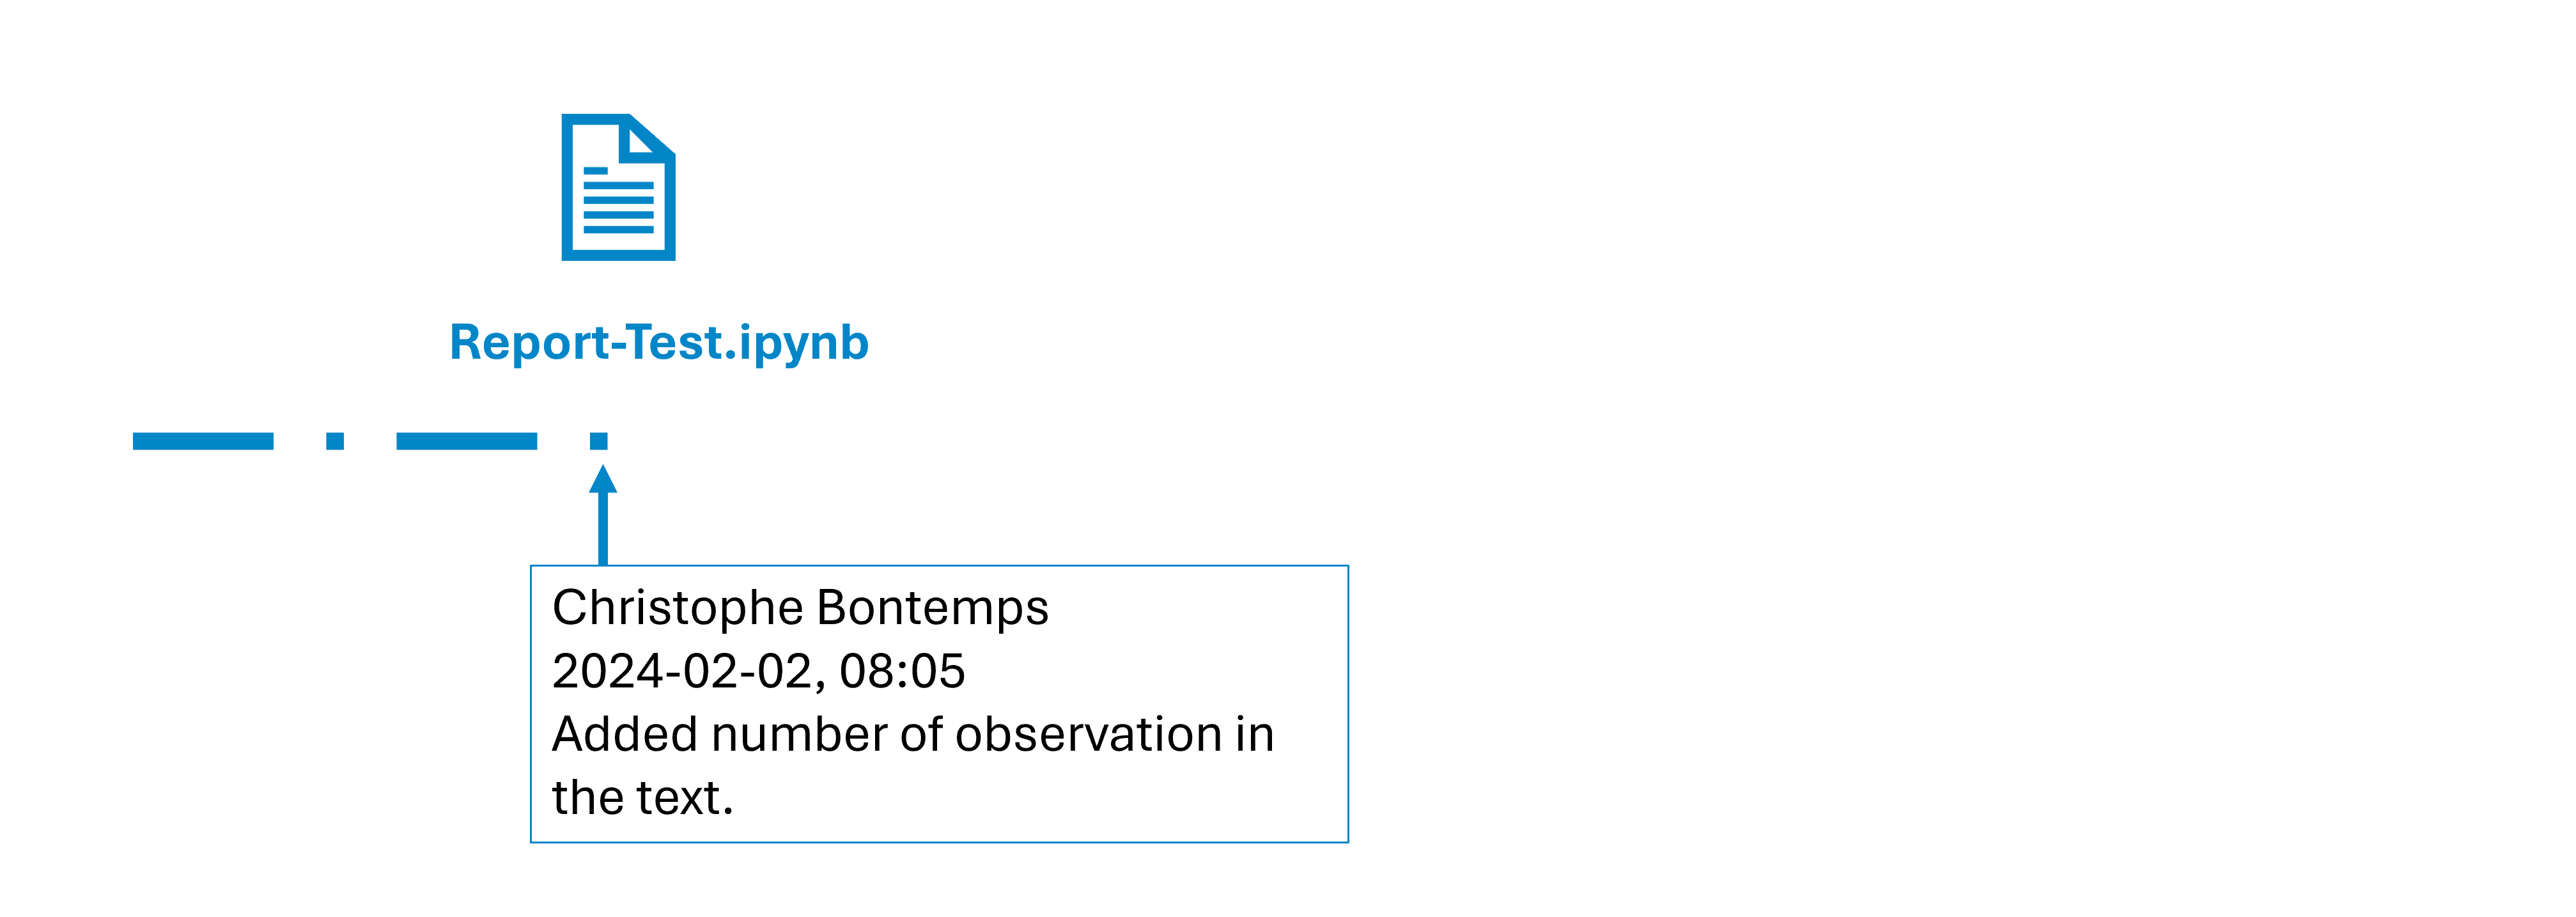
\includegraphics[width = 1.0\textwidth]{FileLife2.png} \\ }
   \only<3> {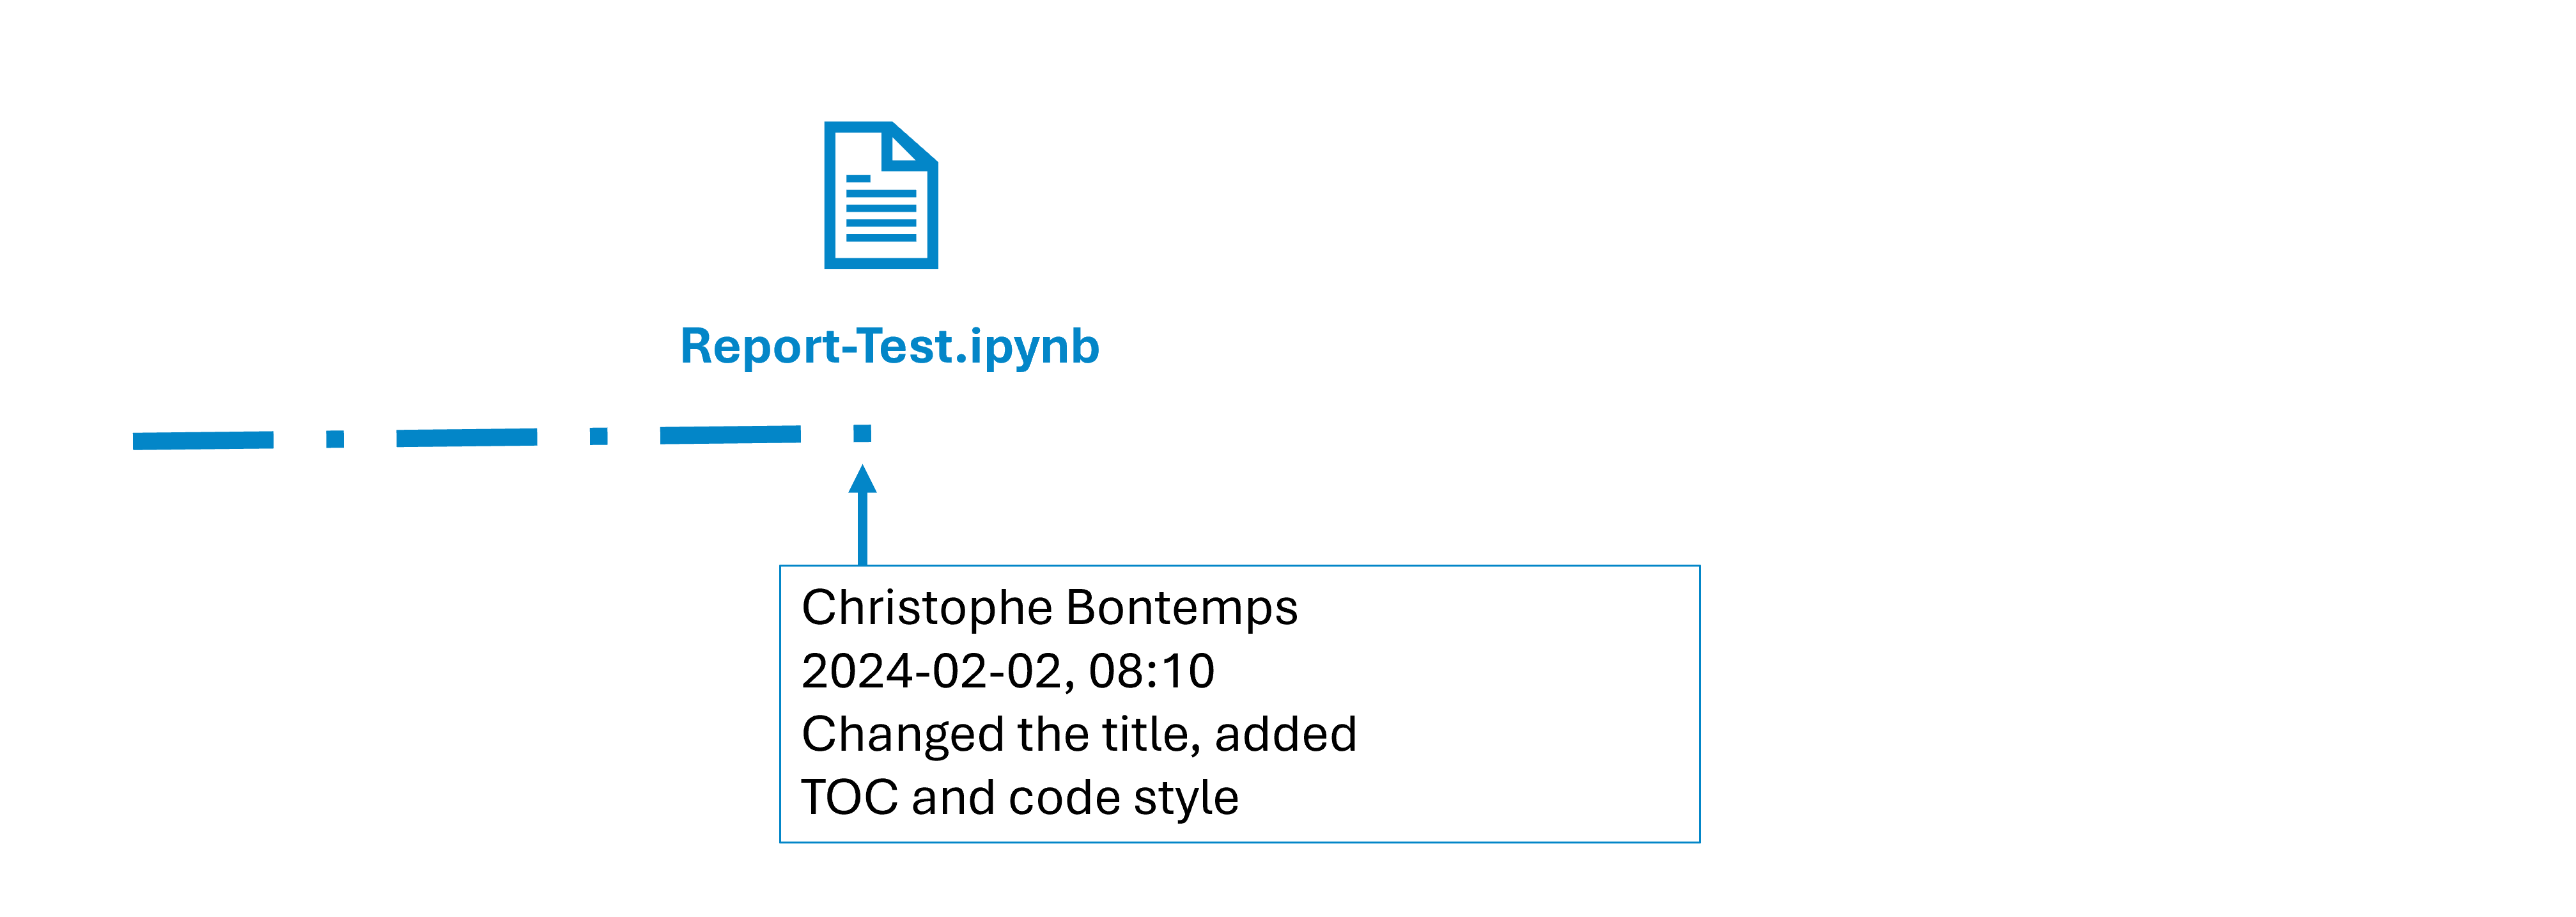
\includegraphics[width = 1.0\textwidth]{FileLife3.png} \\ }
   \only<4> {
\includegraphics[width = 1.0\textwidth]{FileLife4.png} \\ }
   \only<5> {
\includegraphics[width = 1.0\textwidth]{FileLife5.png} \\ }
   \only<6> {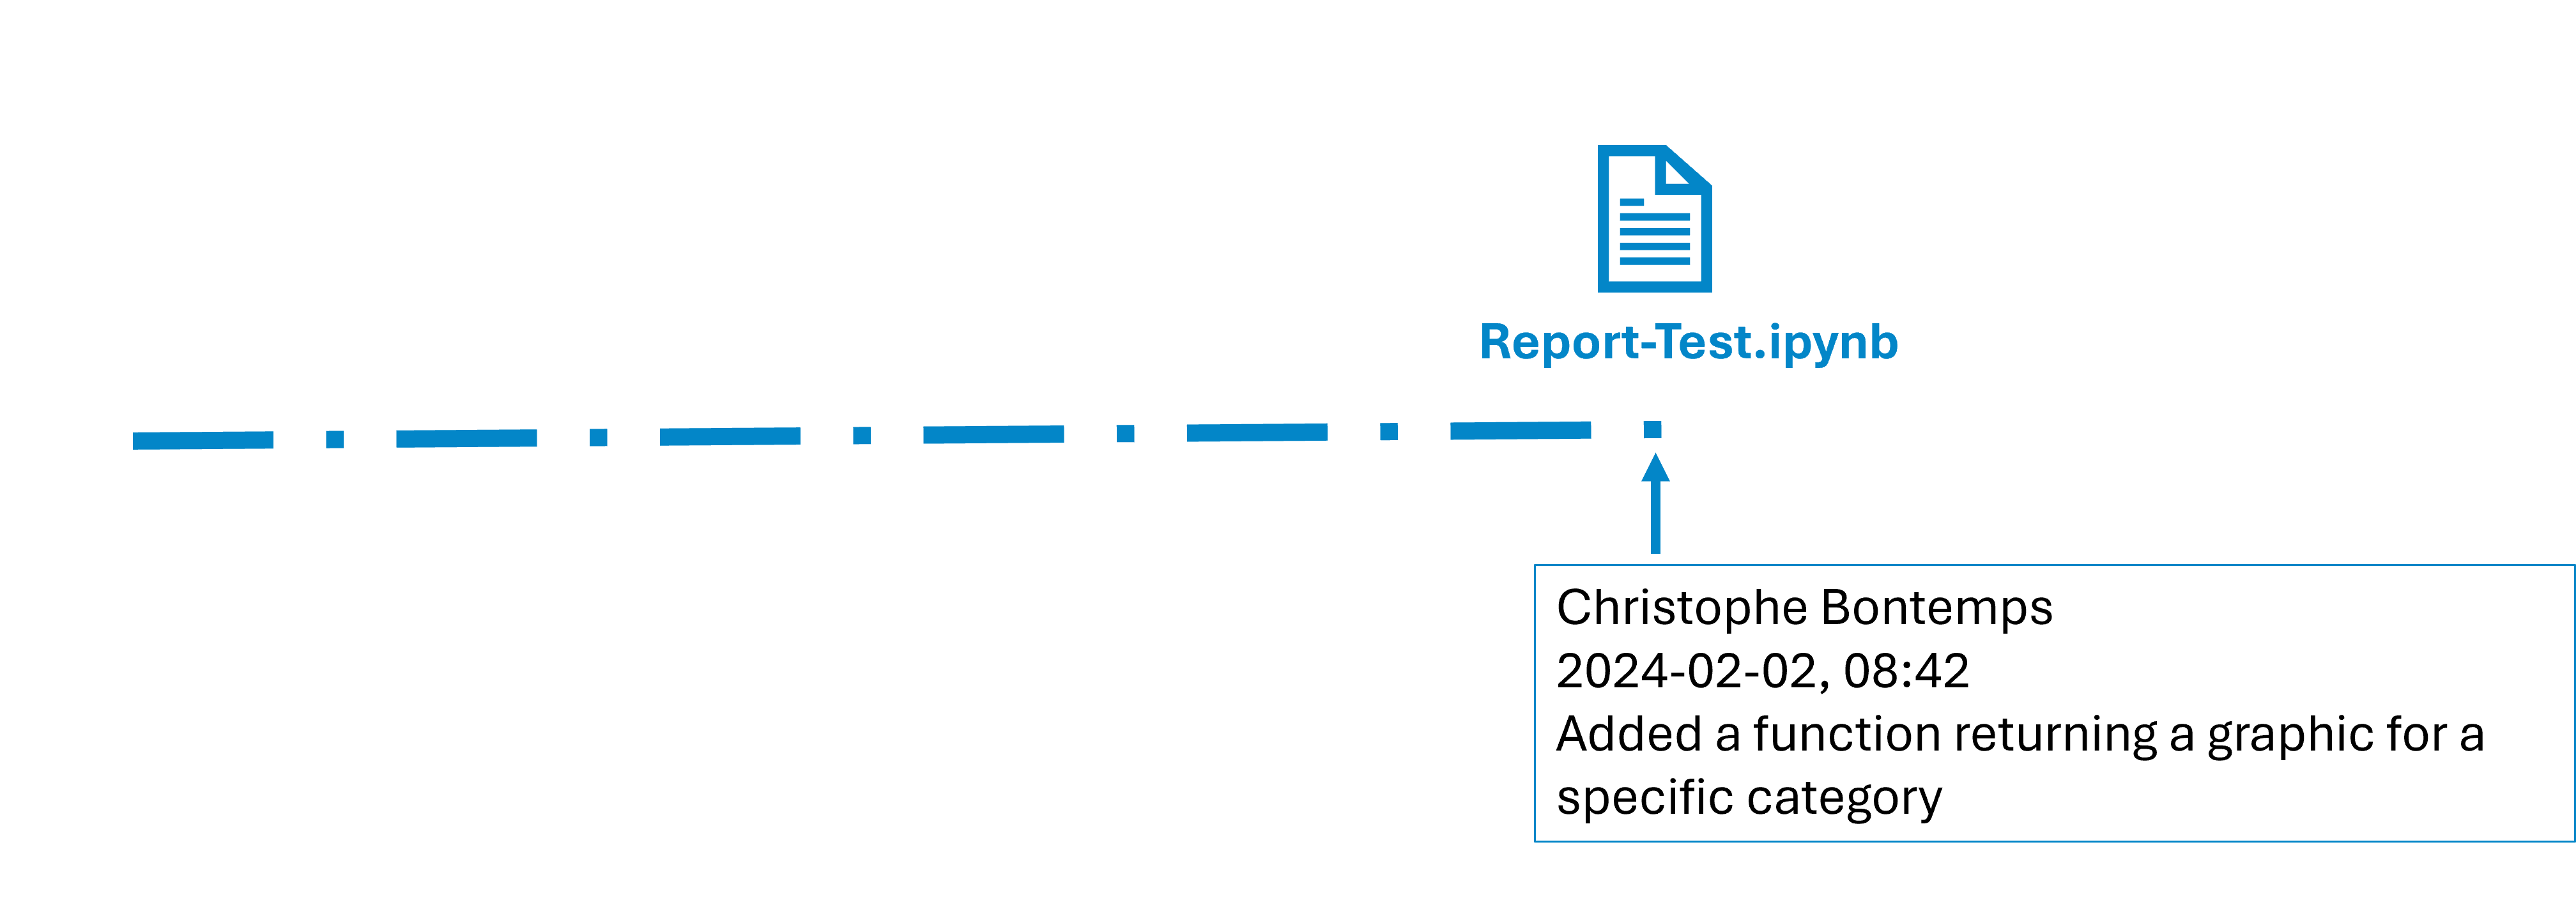
\includegraphics[width = 1.0\textwidth]{FileLife6.png} \\ }
   \only<7> {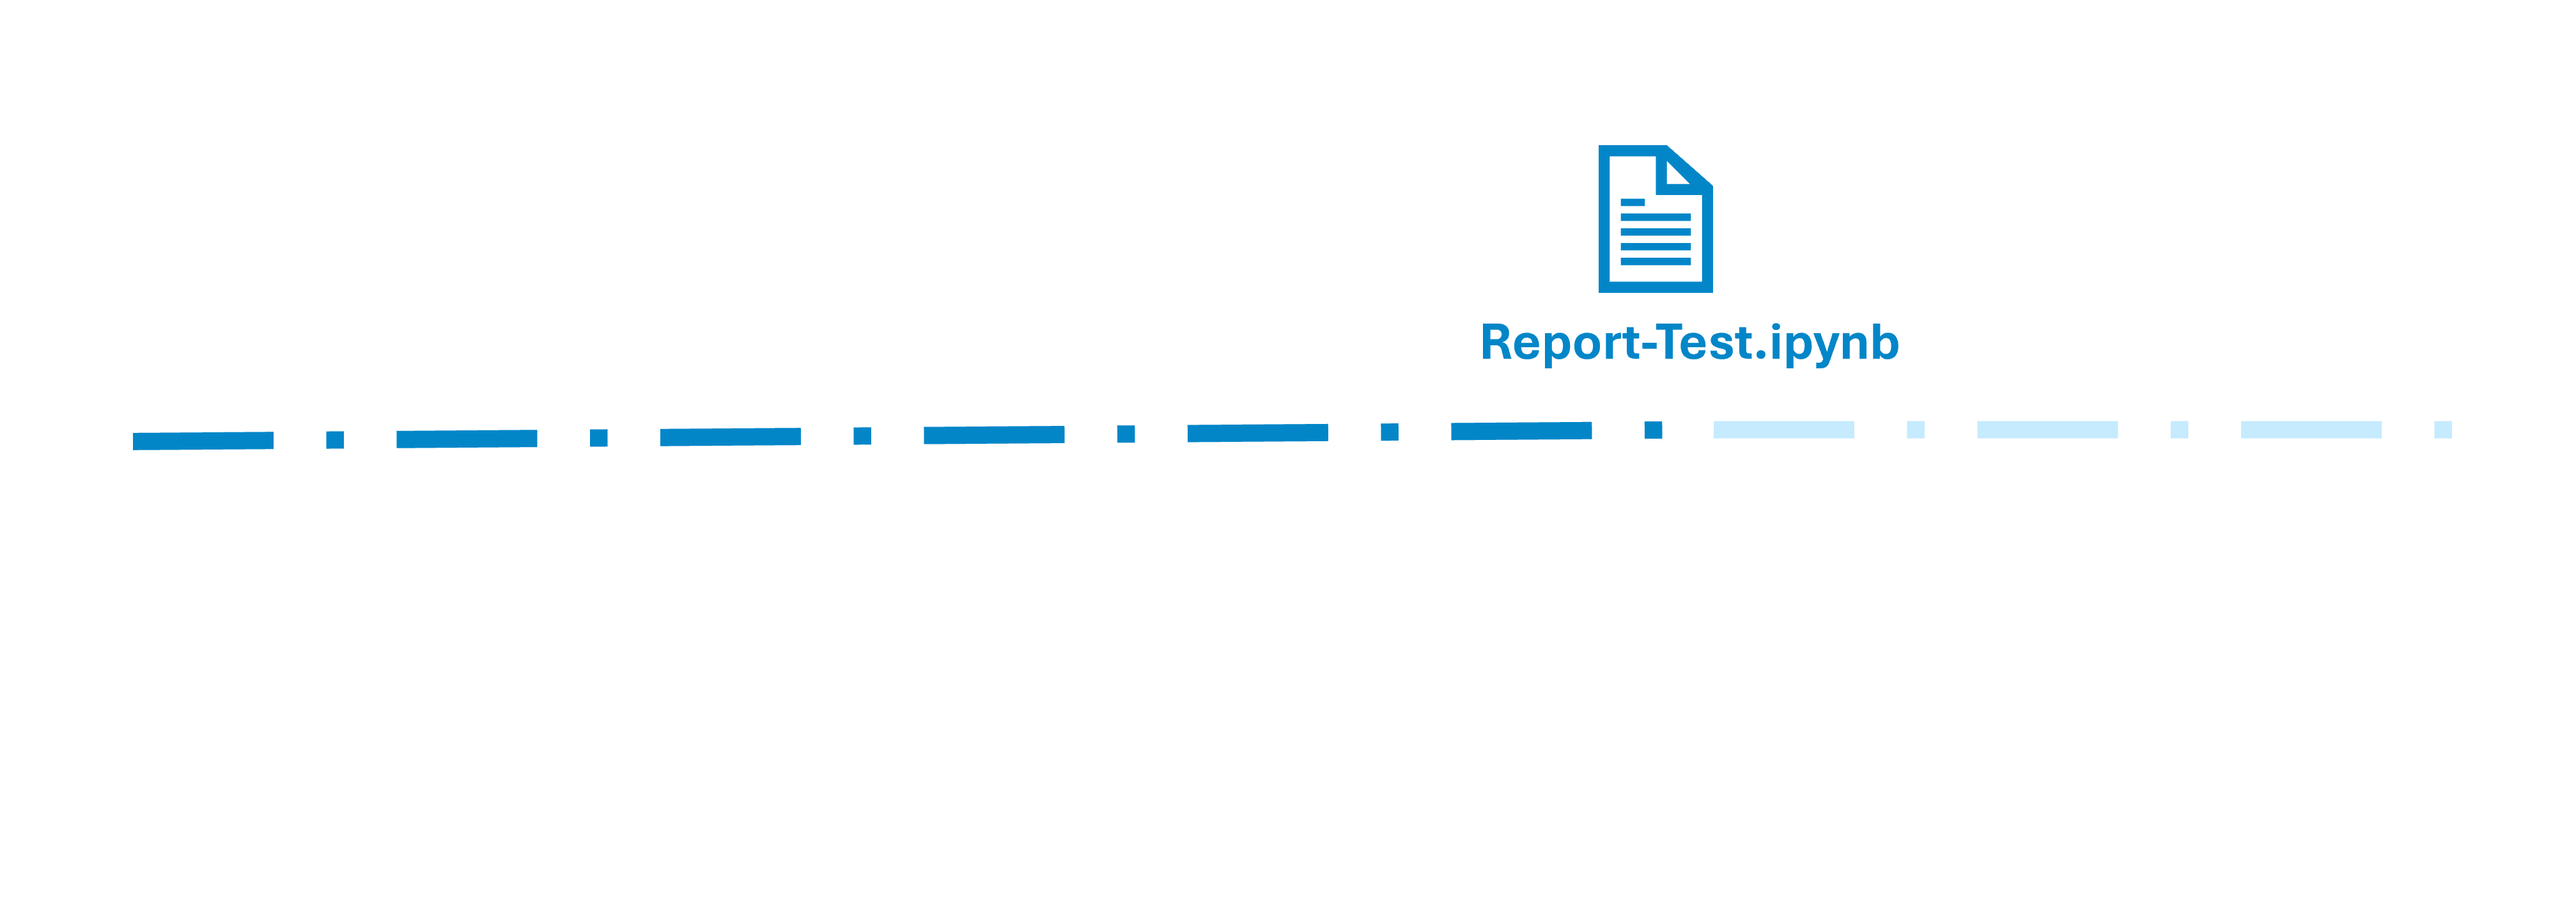
\includegraphics[width = 1.0\textwidth]{FileLife7.png} \\ }
\end{itemize}
\end{center}
\end{frame}

\begin{frame}{The history of the file is recorded!}
\begin{center}
\begin{itemize}
   \only<1-2> {Each version is documented (with \emph{commits}) \\ }
   \only<1-2> {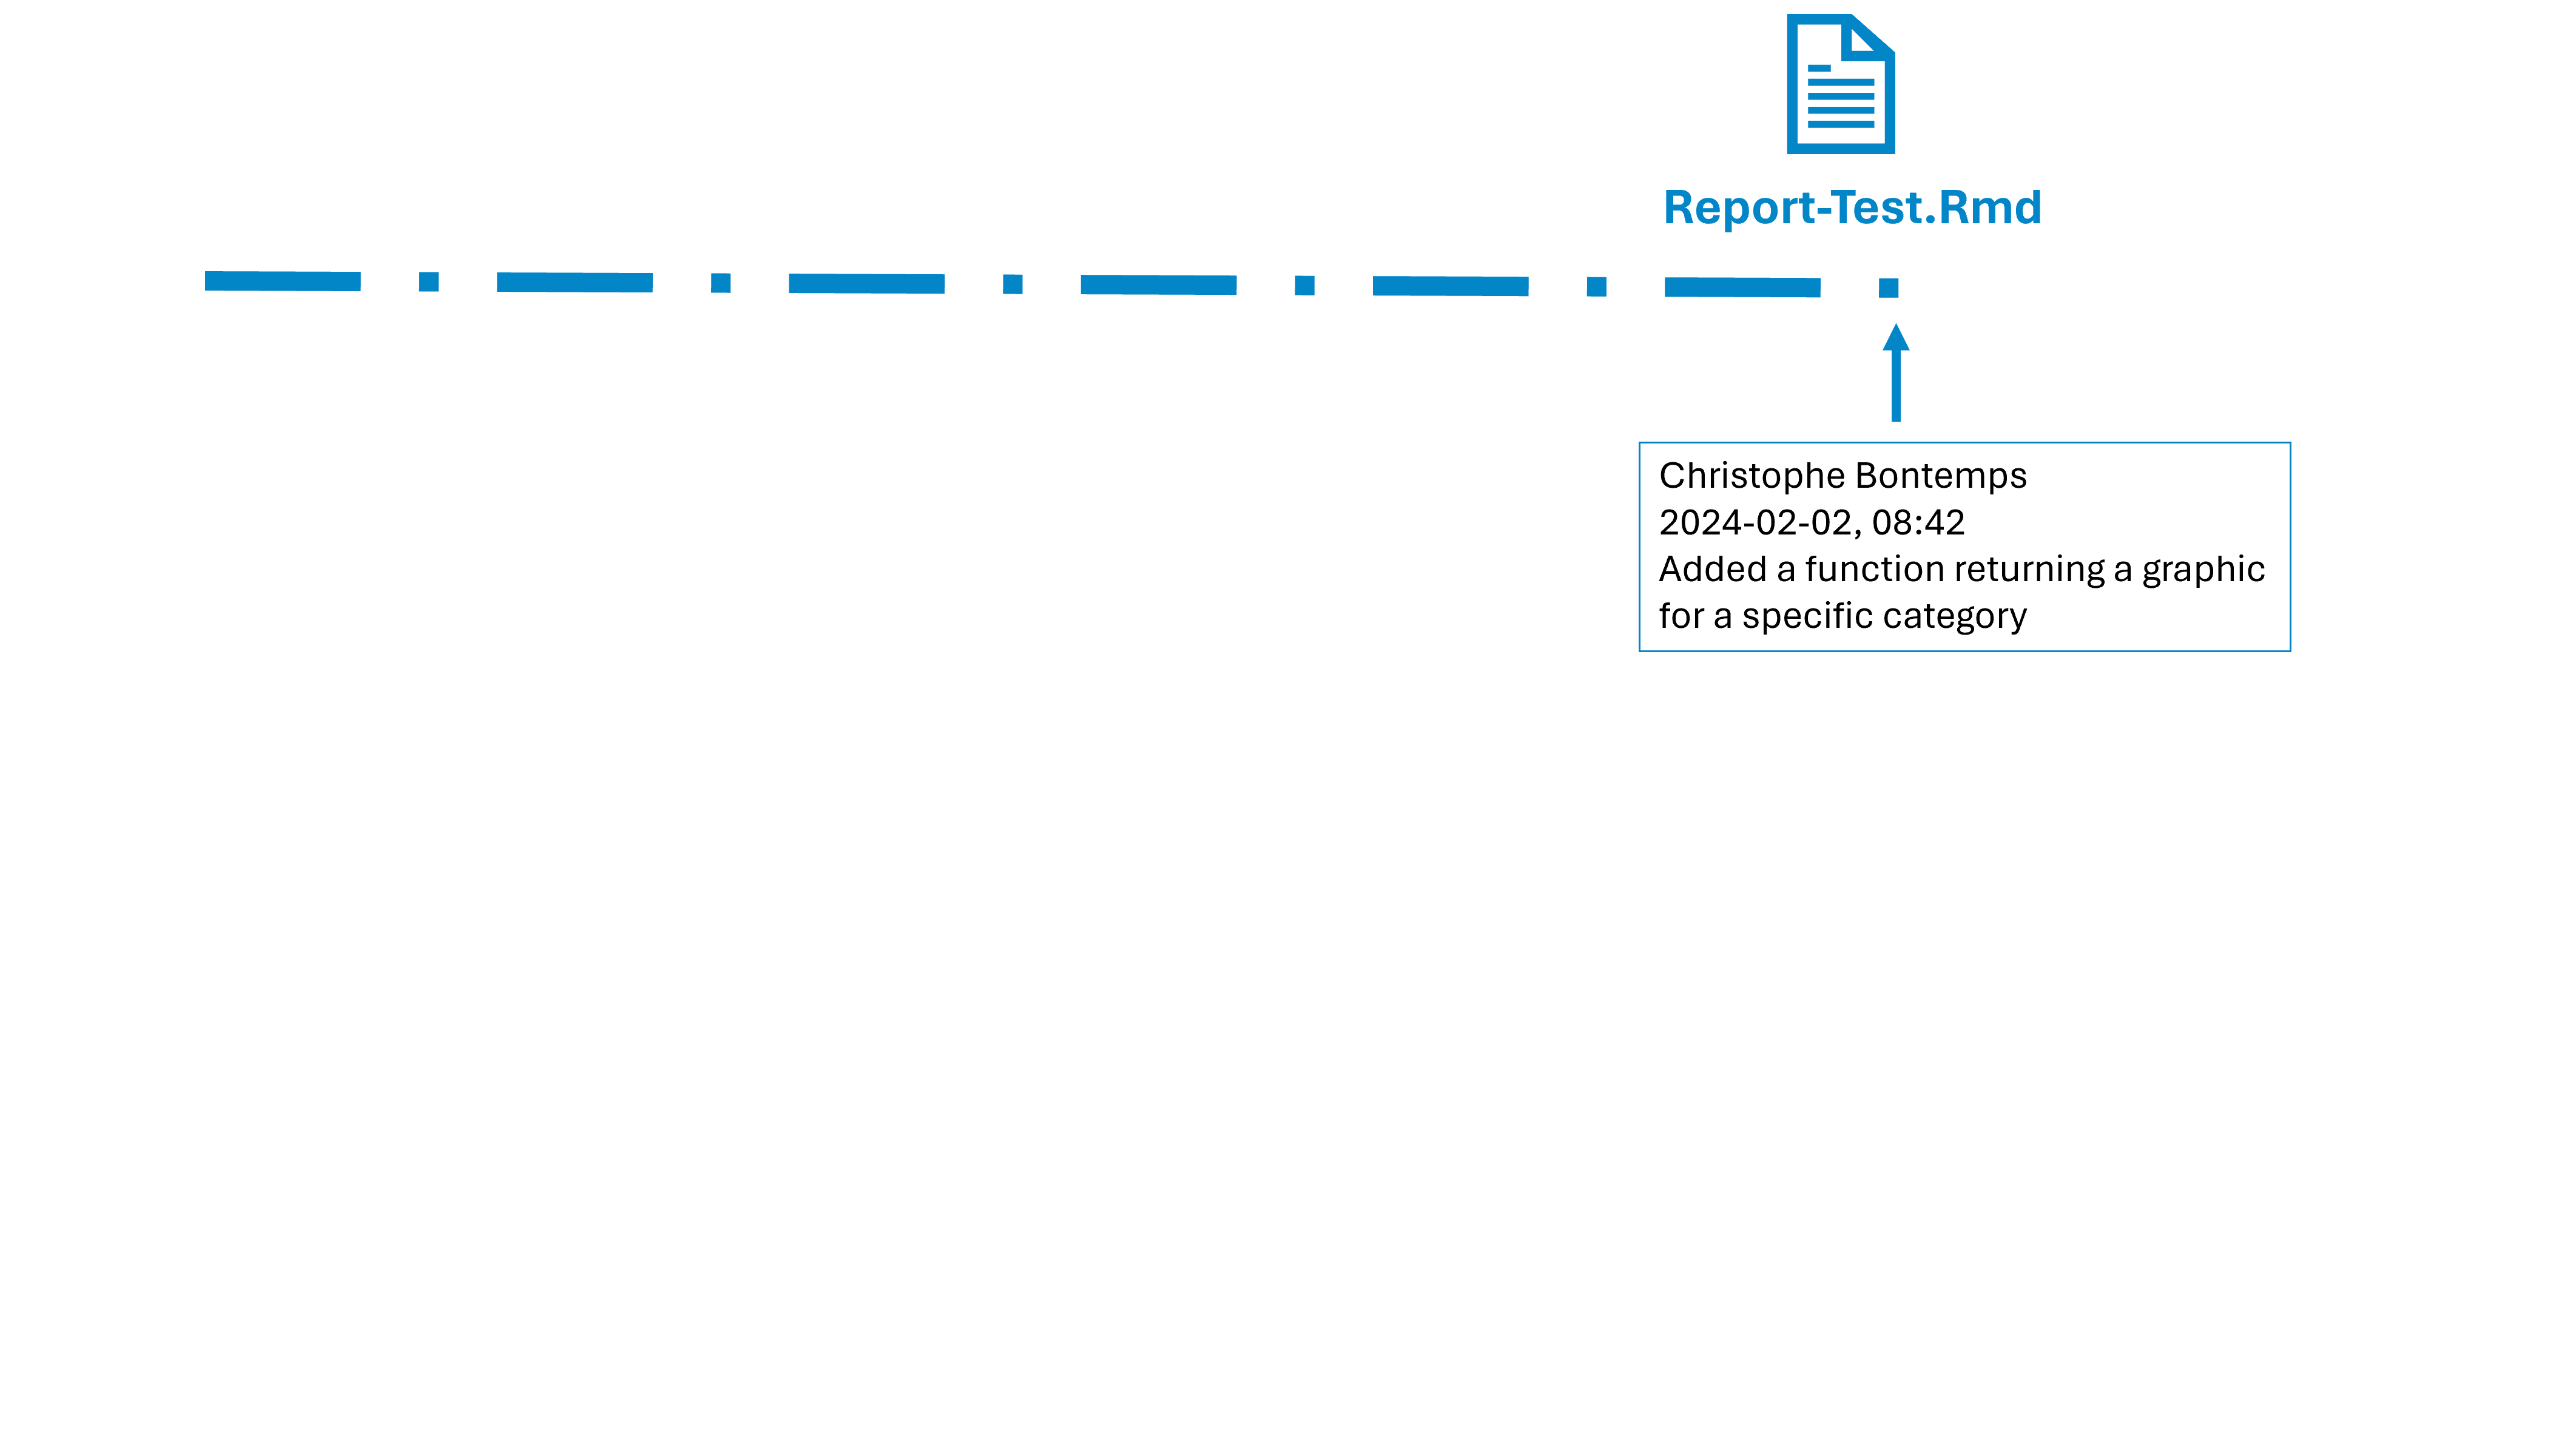
\includegraphics[width = 1.0\textwidth]{FileLifeHistoryEnd.png} \\ }
   \only<3-4> {Each version embeds the full history!  }
   \only<3-4> {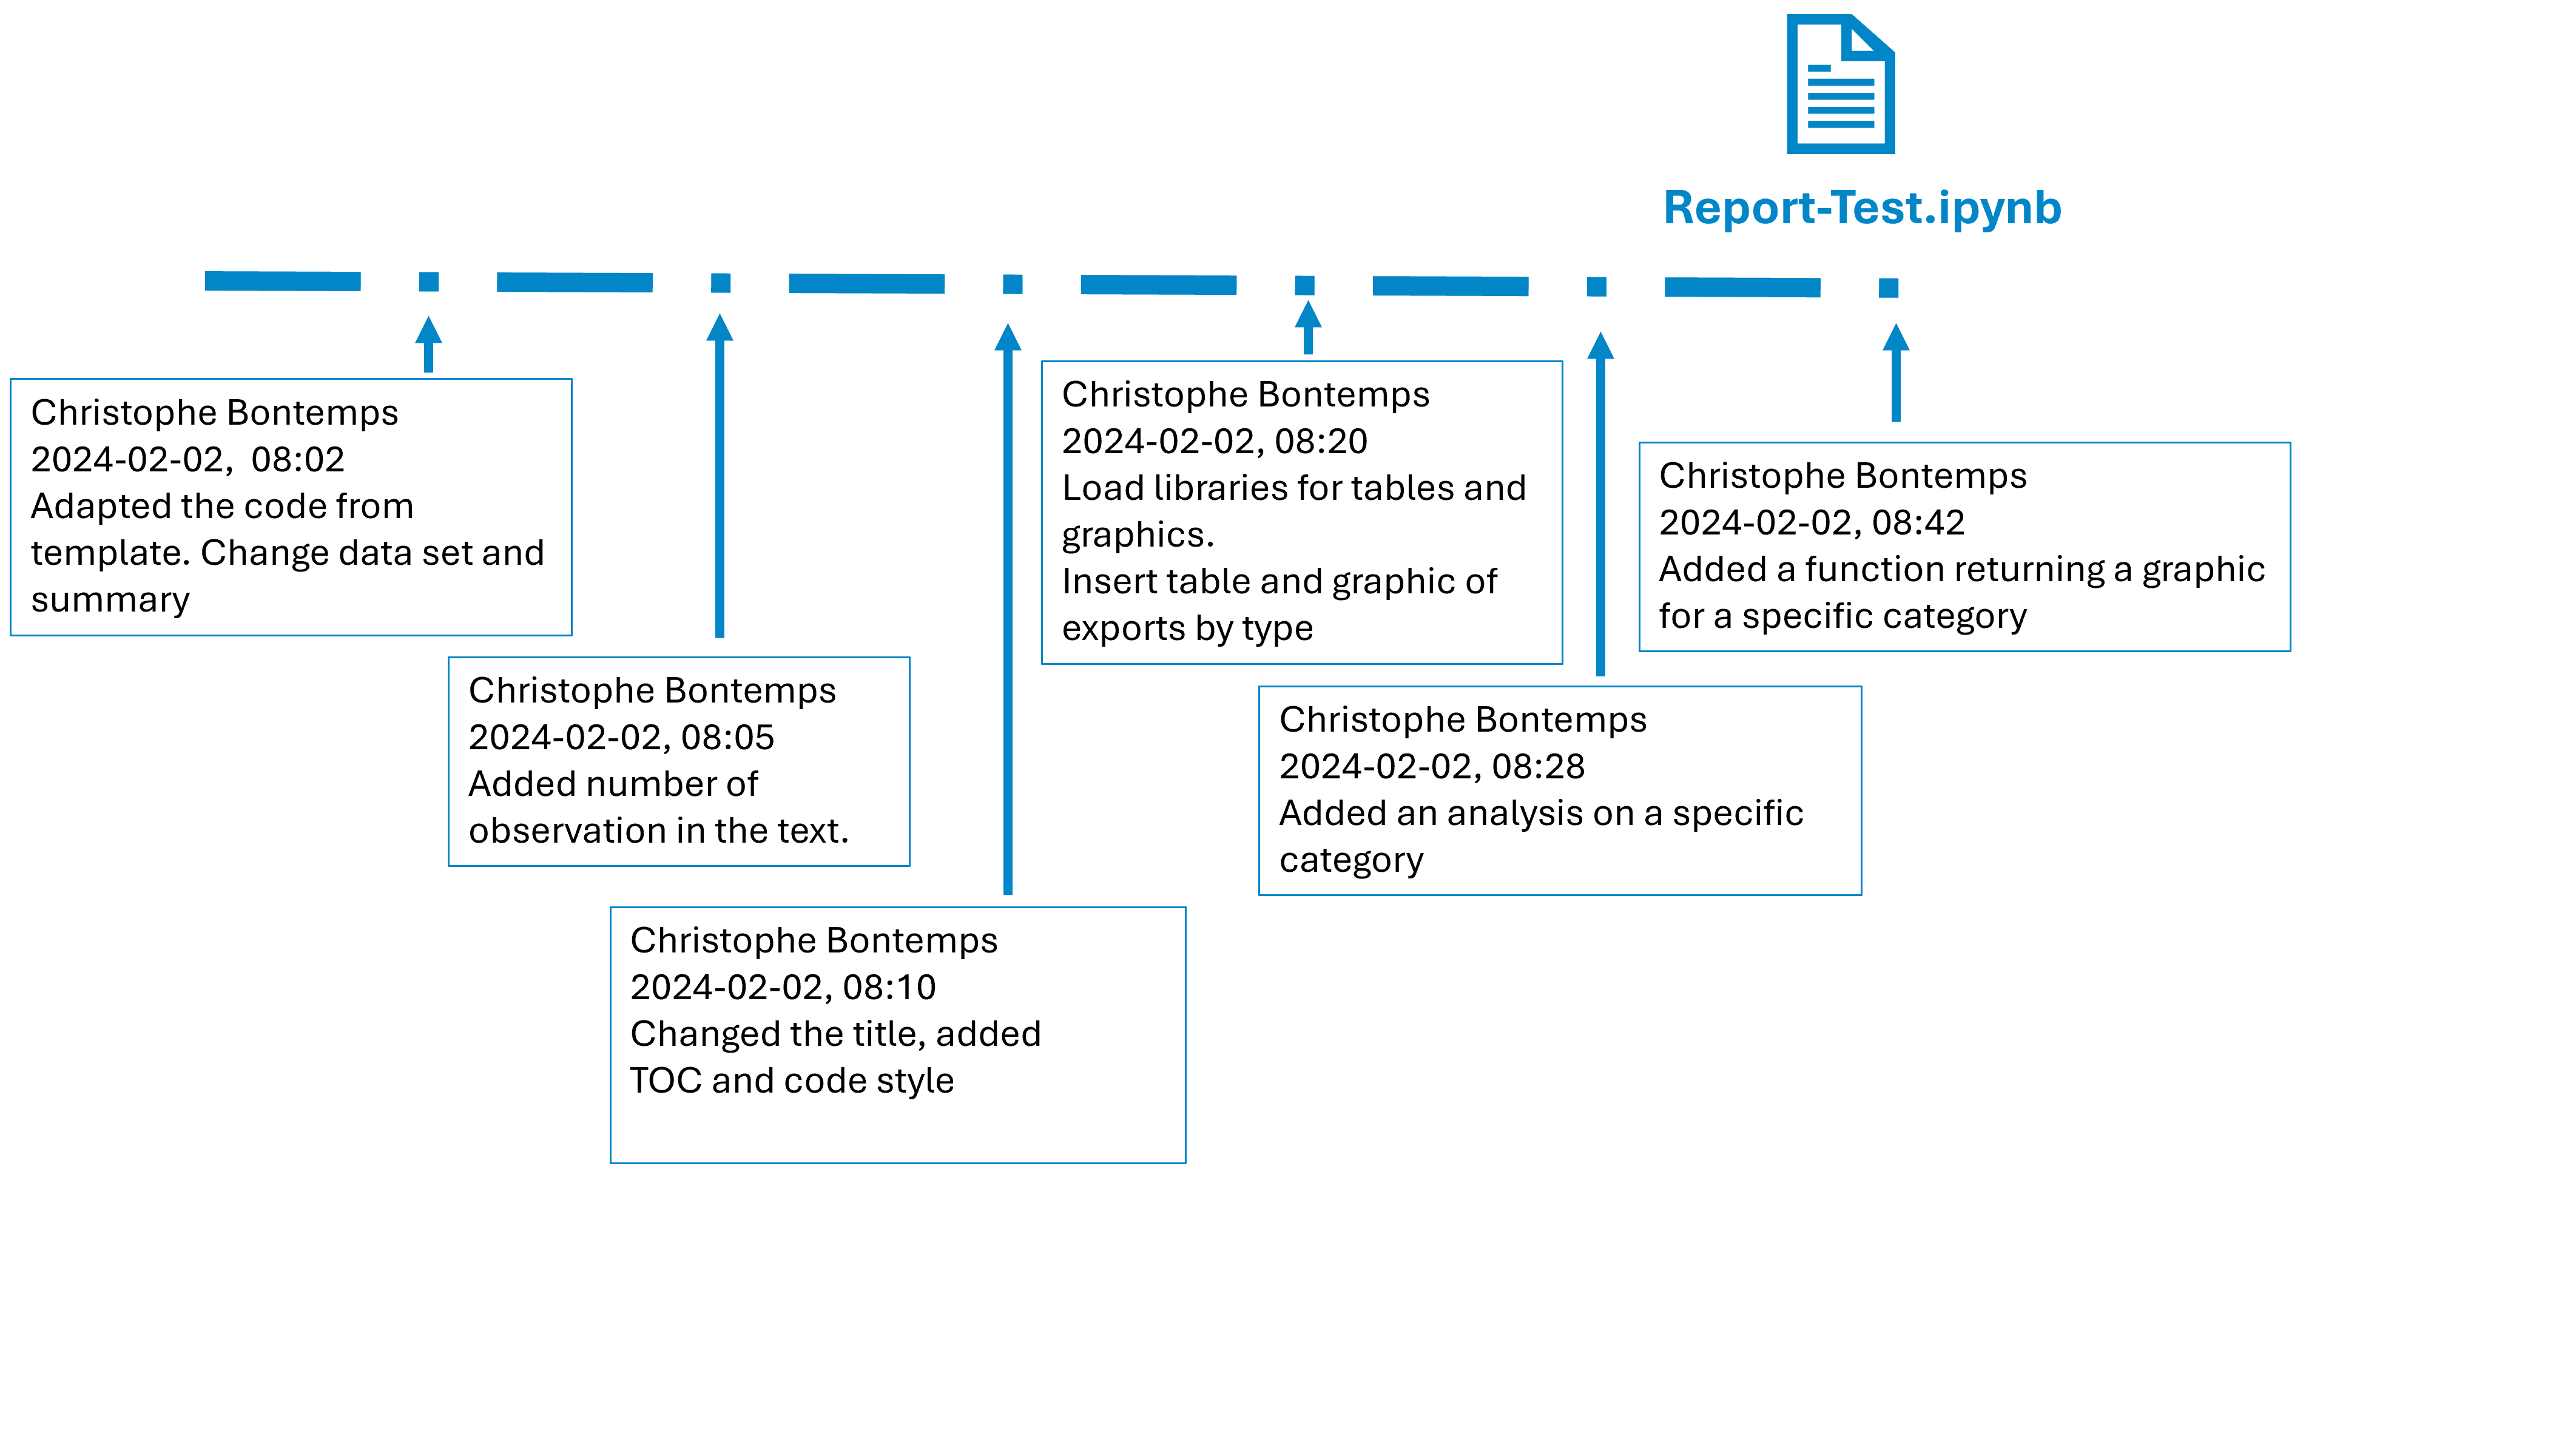
\includegraphics[width = 1.0\textwidth]{FileLifeHistoryFull.png} \\ }
\end{itemize}
\end{center}
\end{frame}

\begin{frame}{Going back and "undo" is possible}
\begin{center}
\begin{itemize}
   \only<1-2> {It is possible to review previous version... \\ }
   \only<1-2> {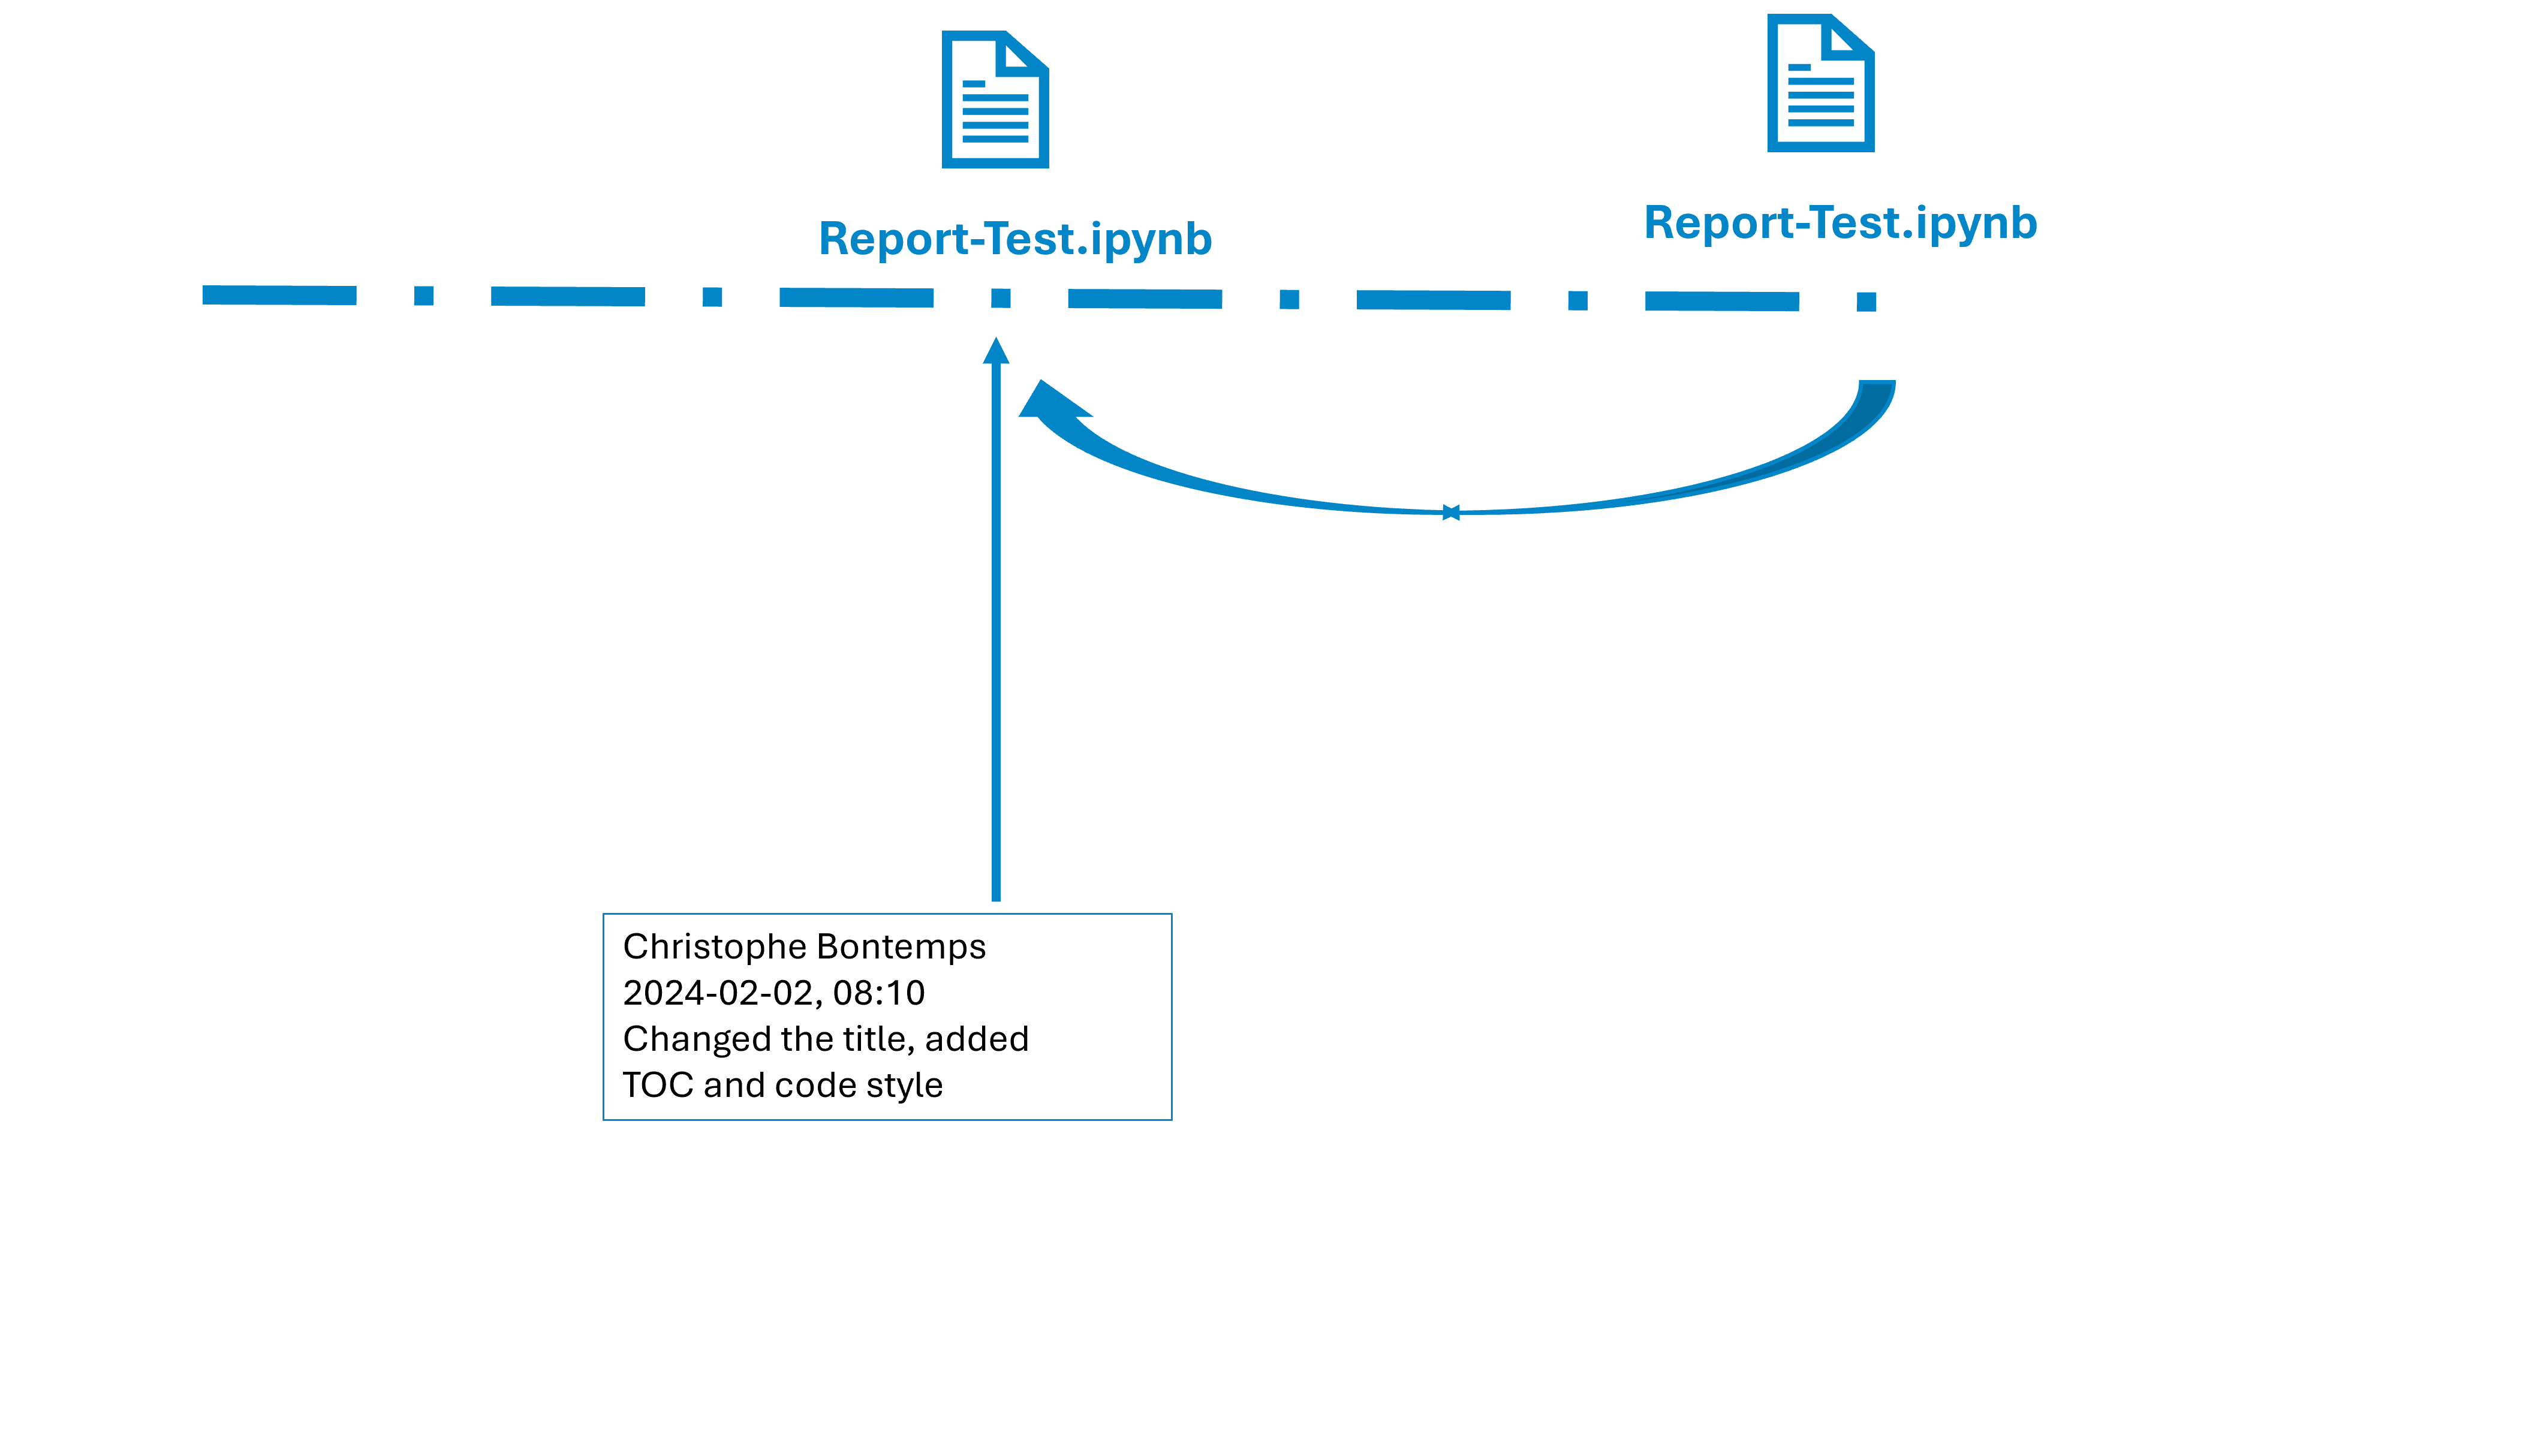
\includegraphics[width = 1.0\textwidth]{FileLifeBack.png} \\ }
   \only<3-4> {...to compare the changes...  }
   \only<3-4> {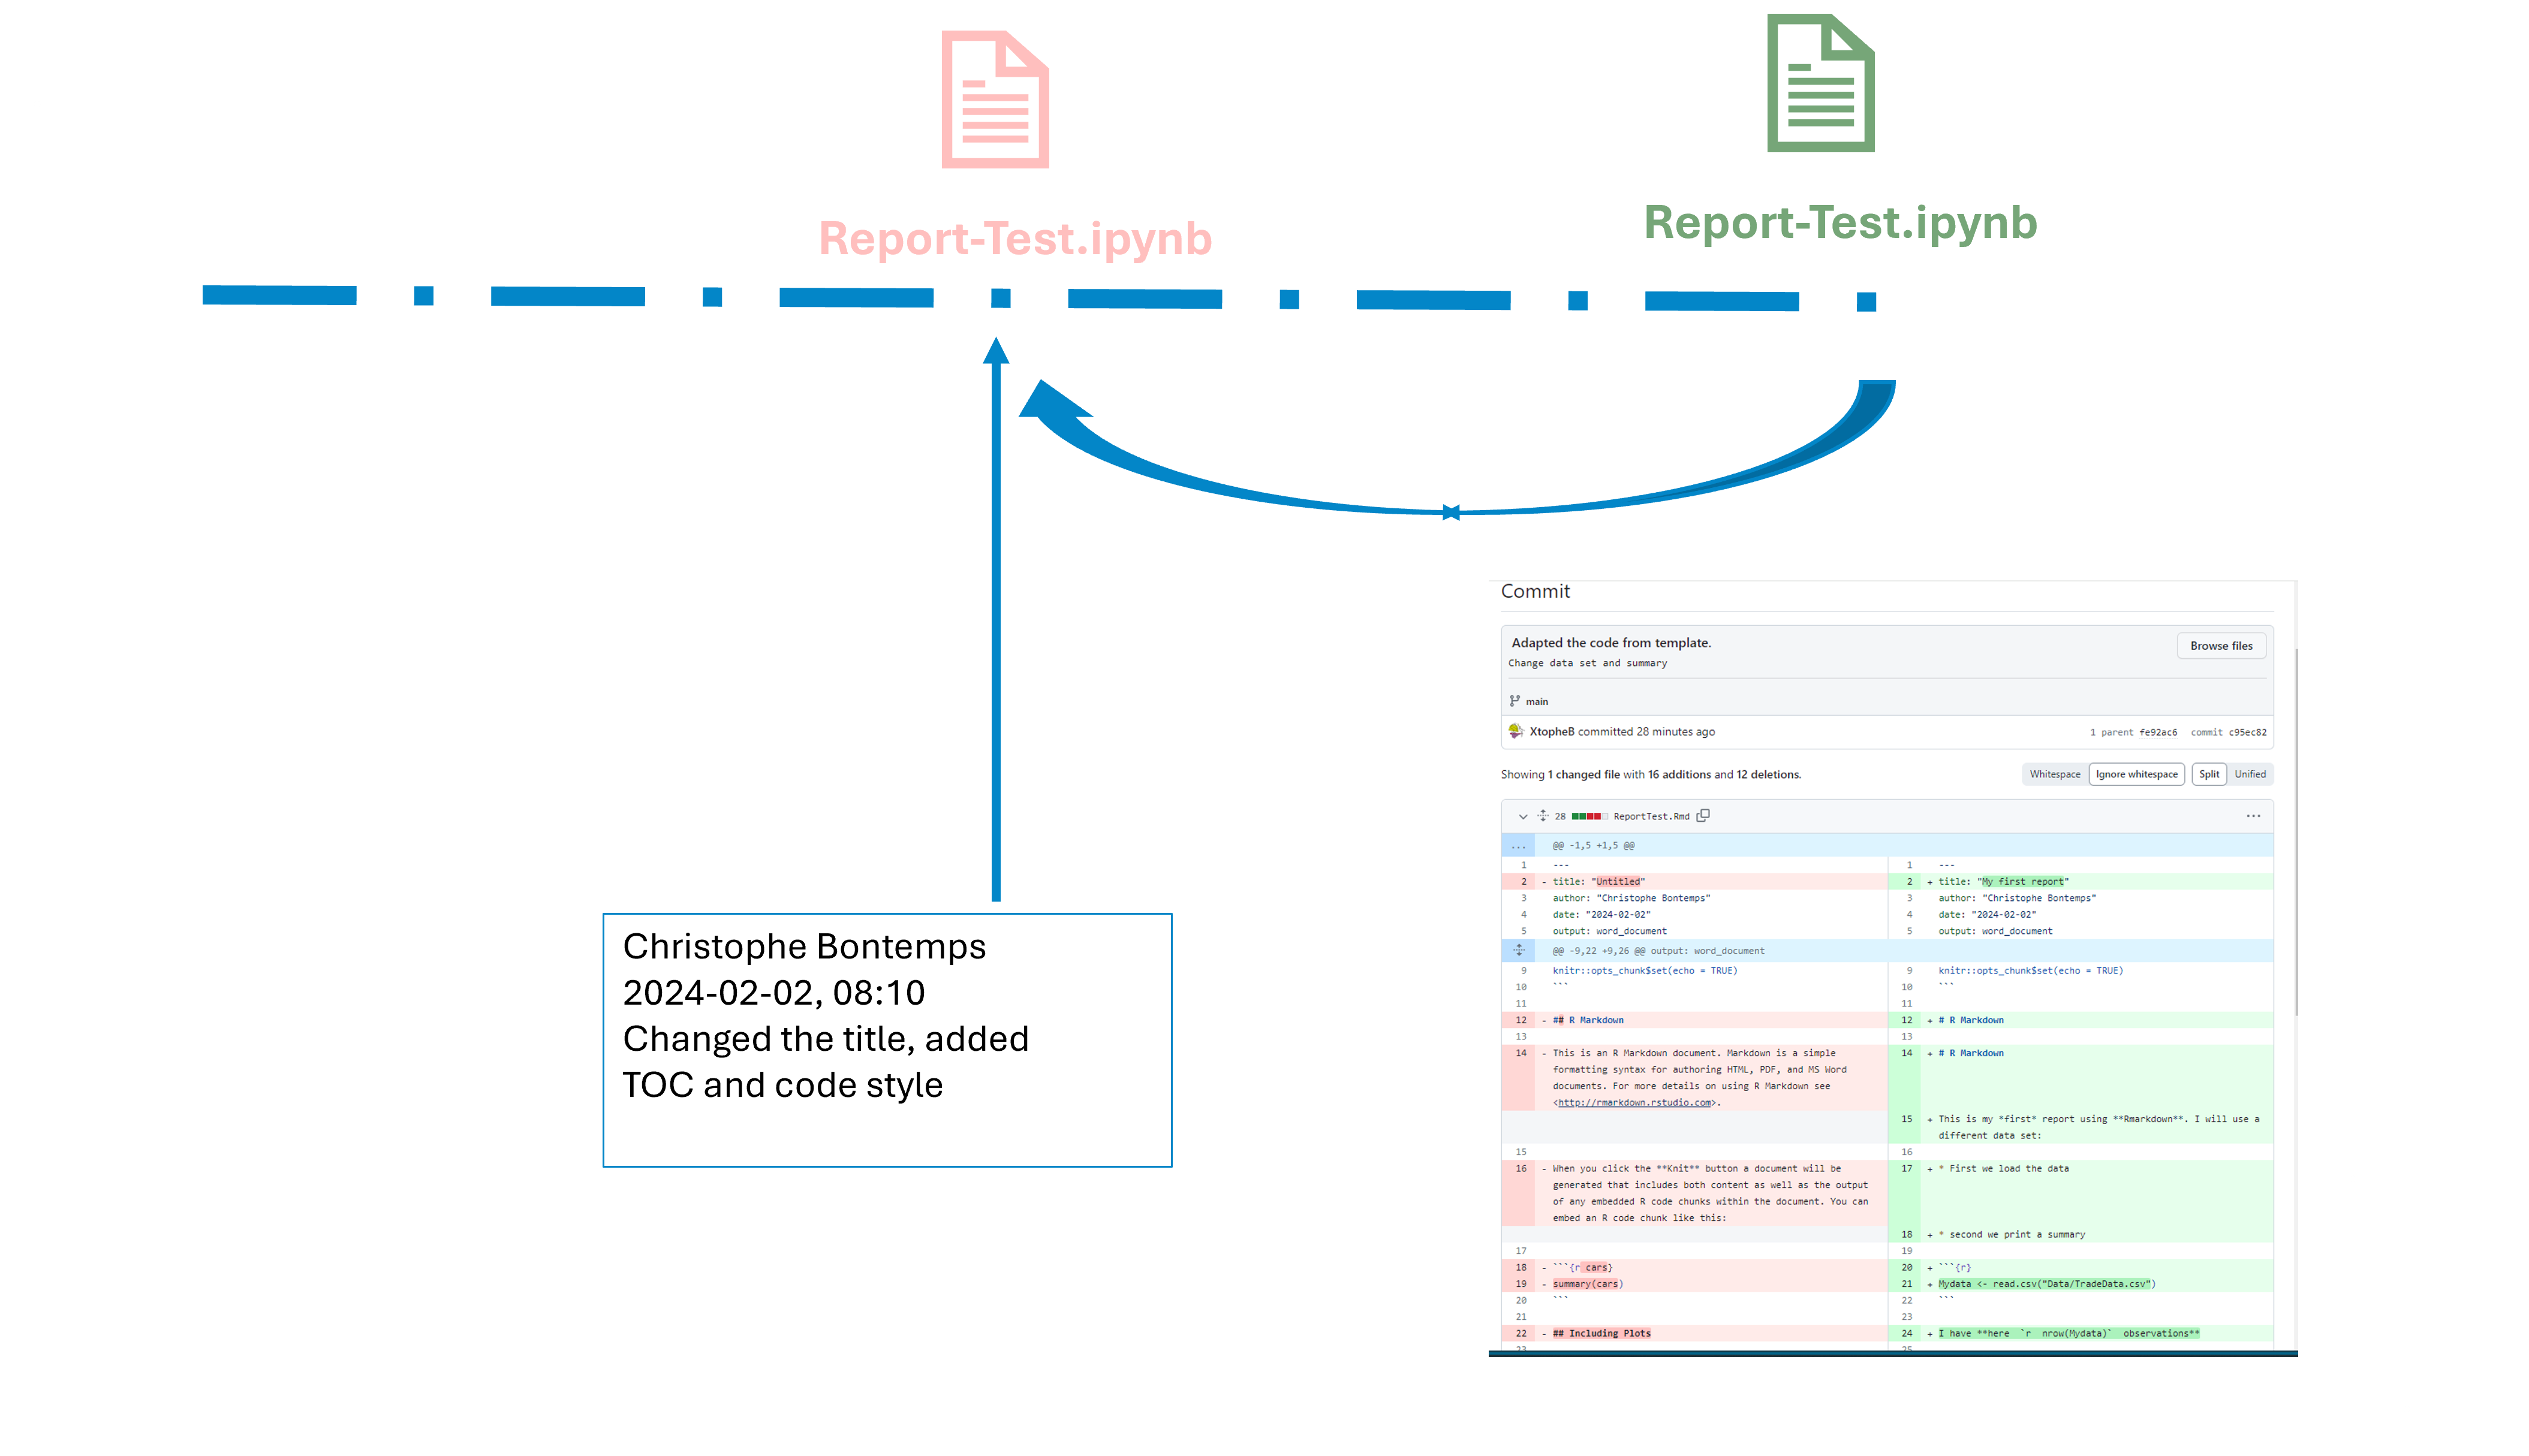
\includegraphics[width = 1.0\textwidth]{FileLifeDiff.png} \\ }
   \only<5-6> {... and to revert  to a  previous version... }
   \only<5-6> {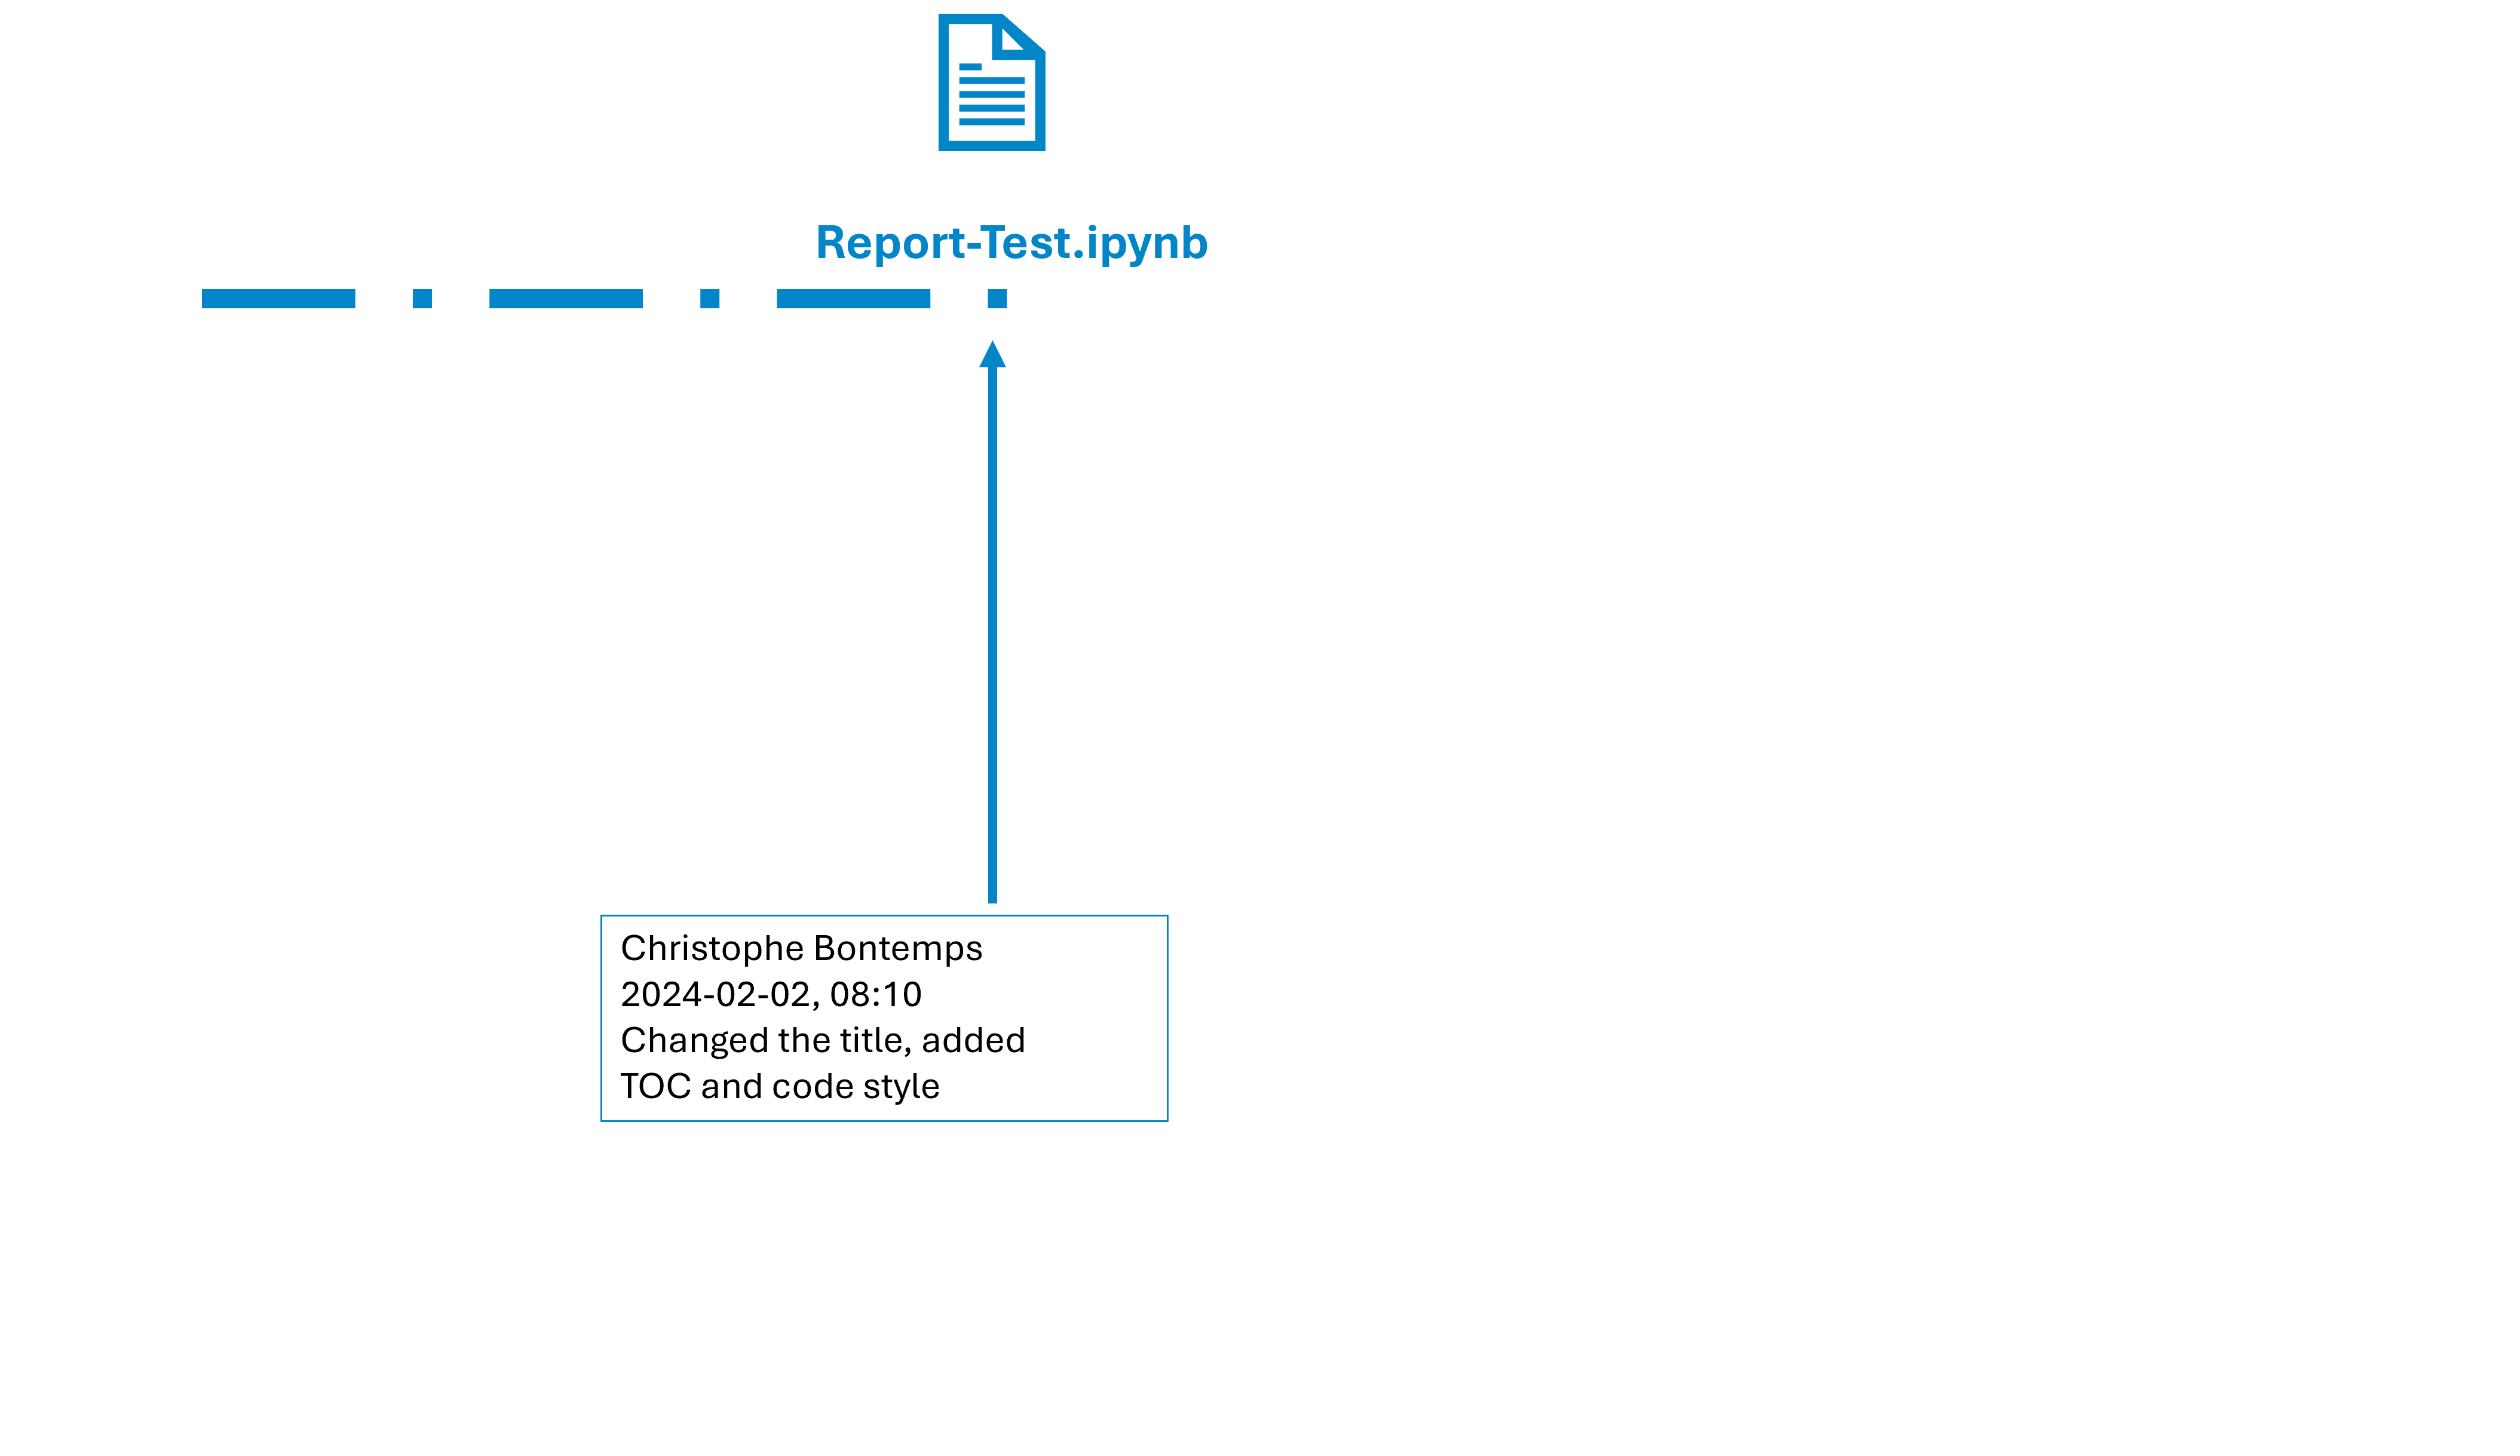
\includegraphics[width = 1.0\textwidth]{FileLifeRevert.png} \\ }
   \only<7-8> {... or \emph{undo} as if nothing happened }
   \only<7-8> {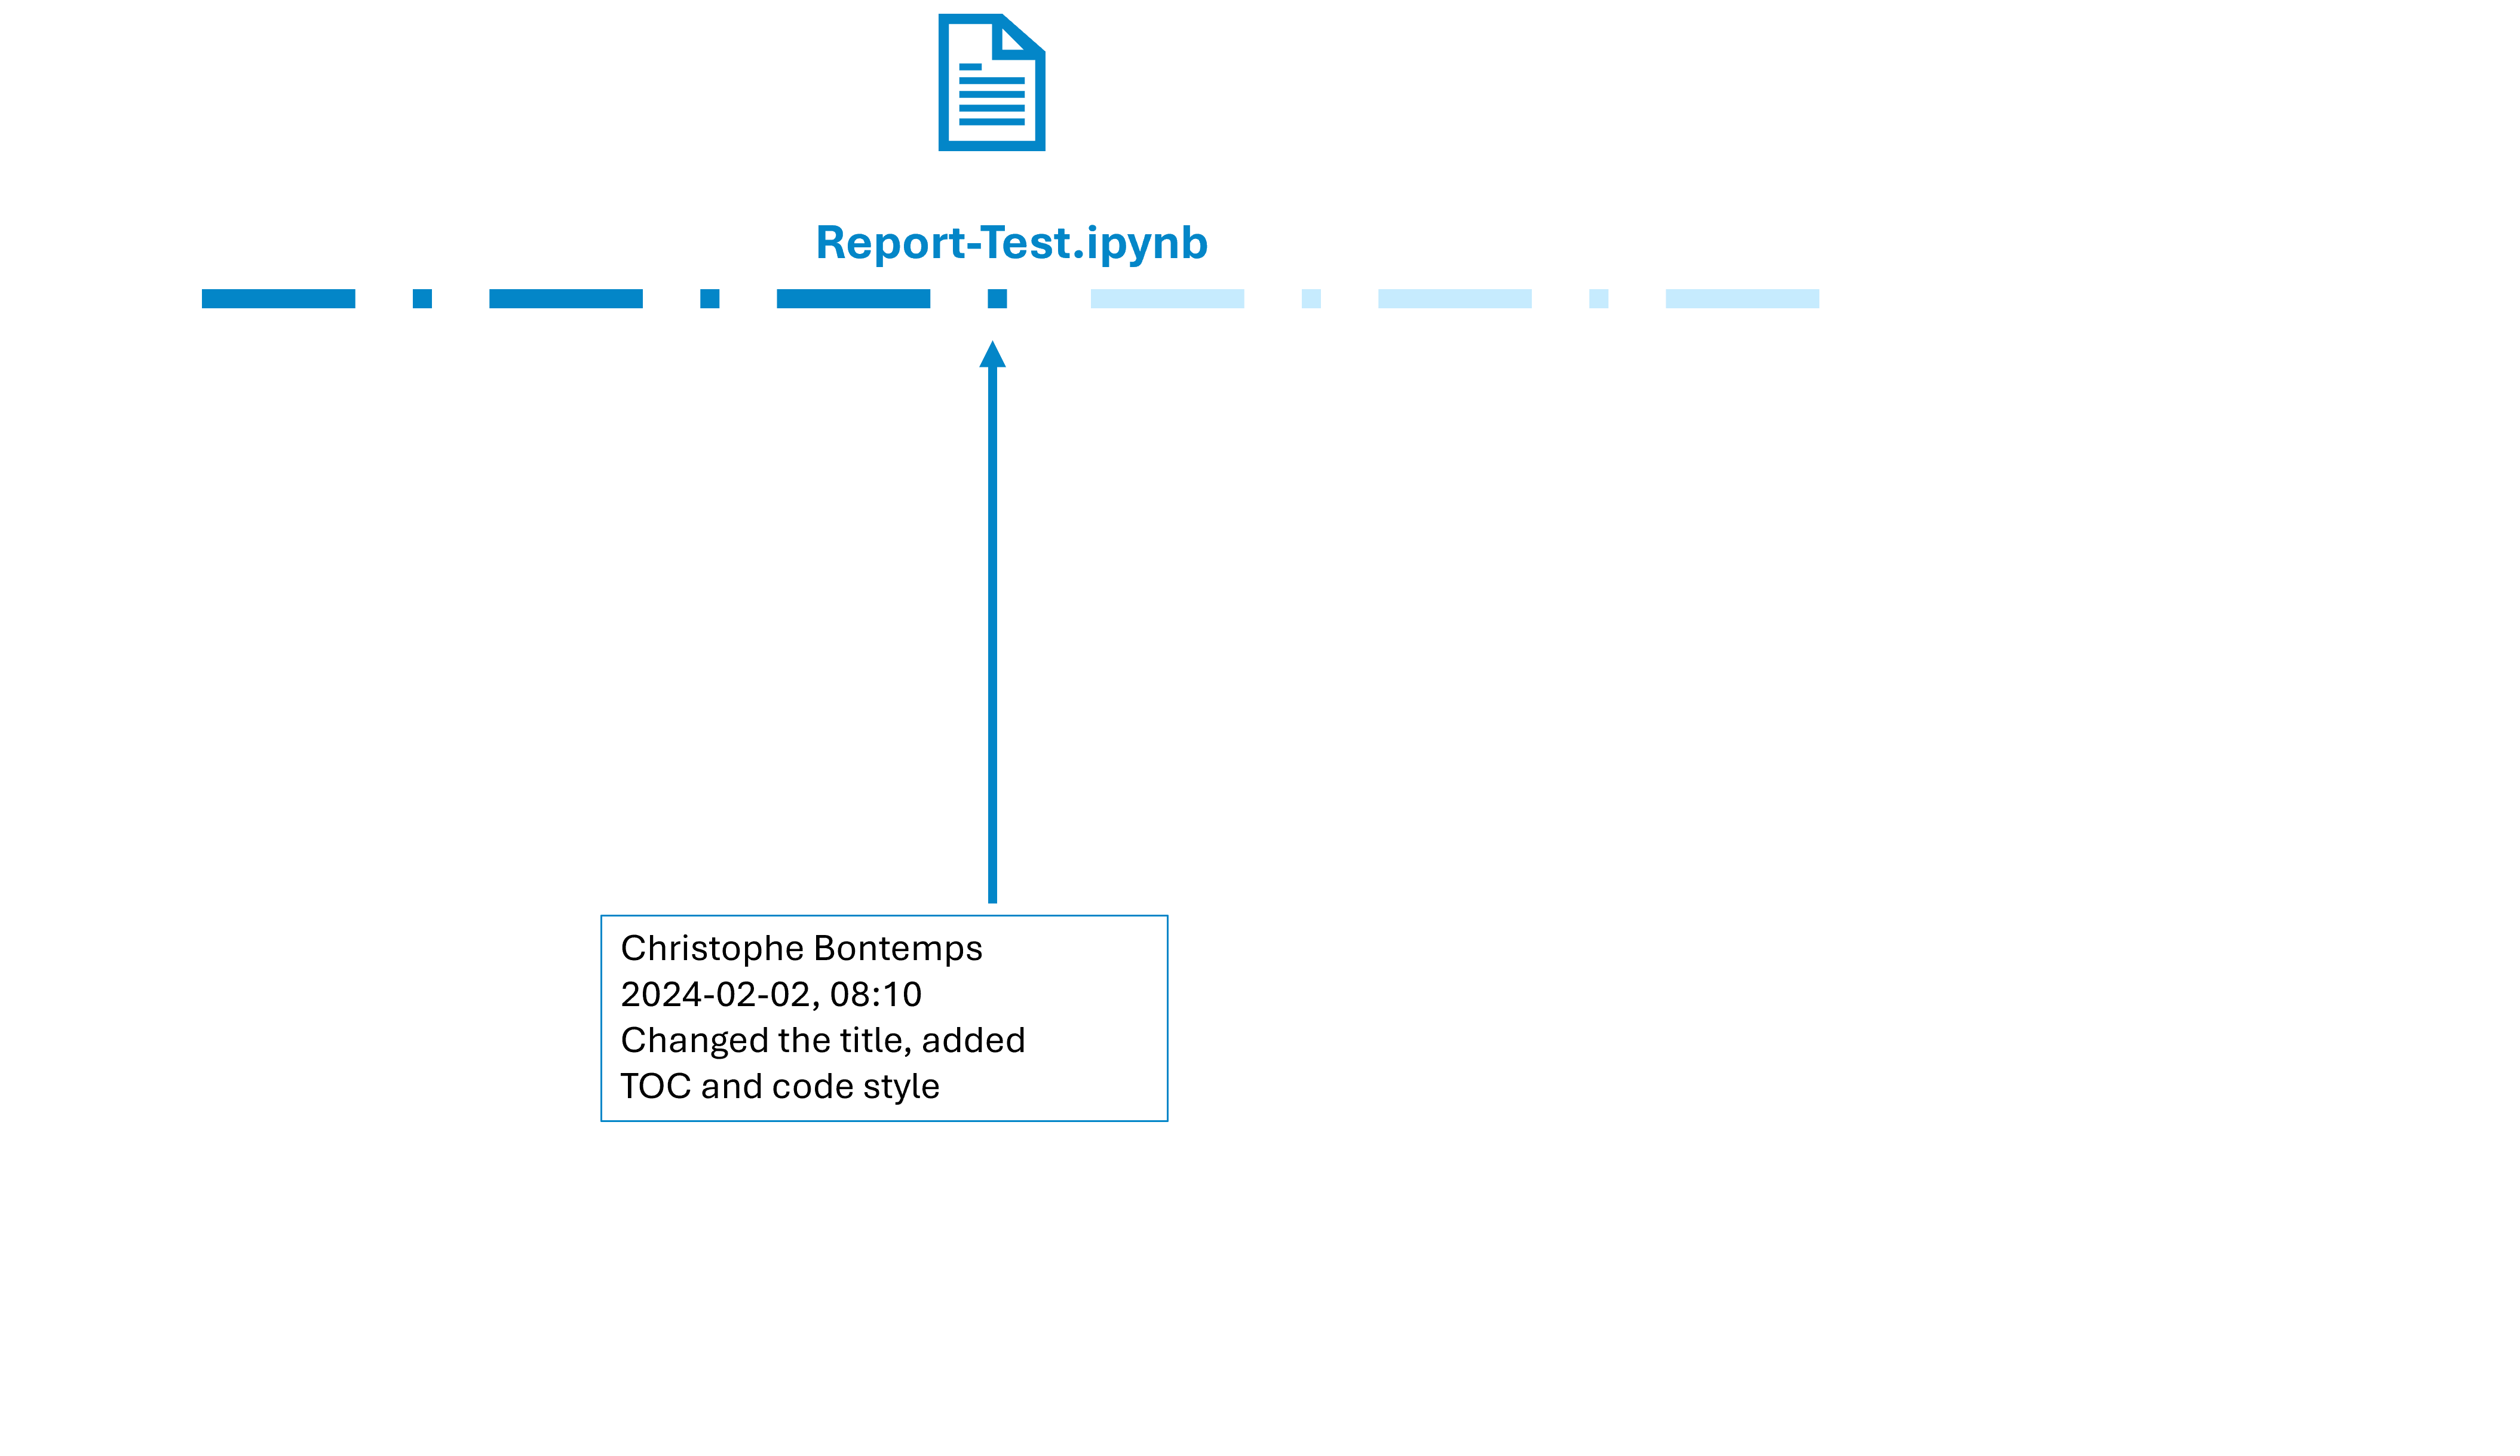
\includegraphics[width = 1.0\textwidth]{FileLifeRevert2.png} \\ }

\end{itemize}
\end{center}
\end{frame}

\begin{frame}
\frametitle{Git for collaborating}
\begin{itemize}
\item[] \textcolor{violet}{\textbf{Alice}} and \textcolor{orange}{\textbf{Bob}} work on the same file\\ \vspace{1cm}
    \only<1>{
\includegraphics[width=1.1\textwidth]{GitSimple1.png} \\  }
    \only<2>{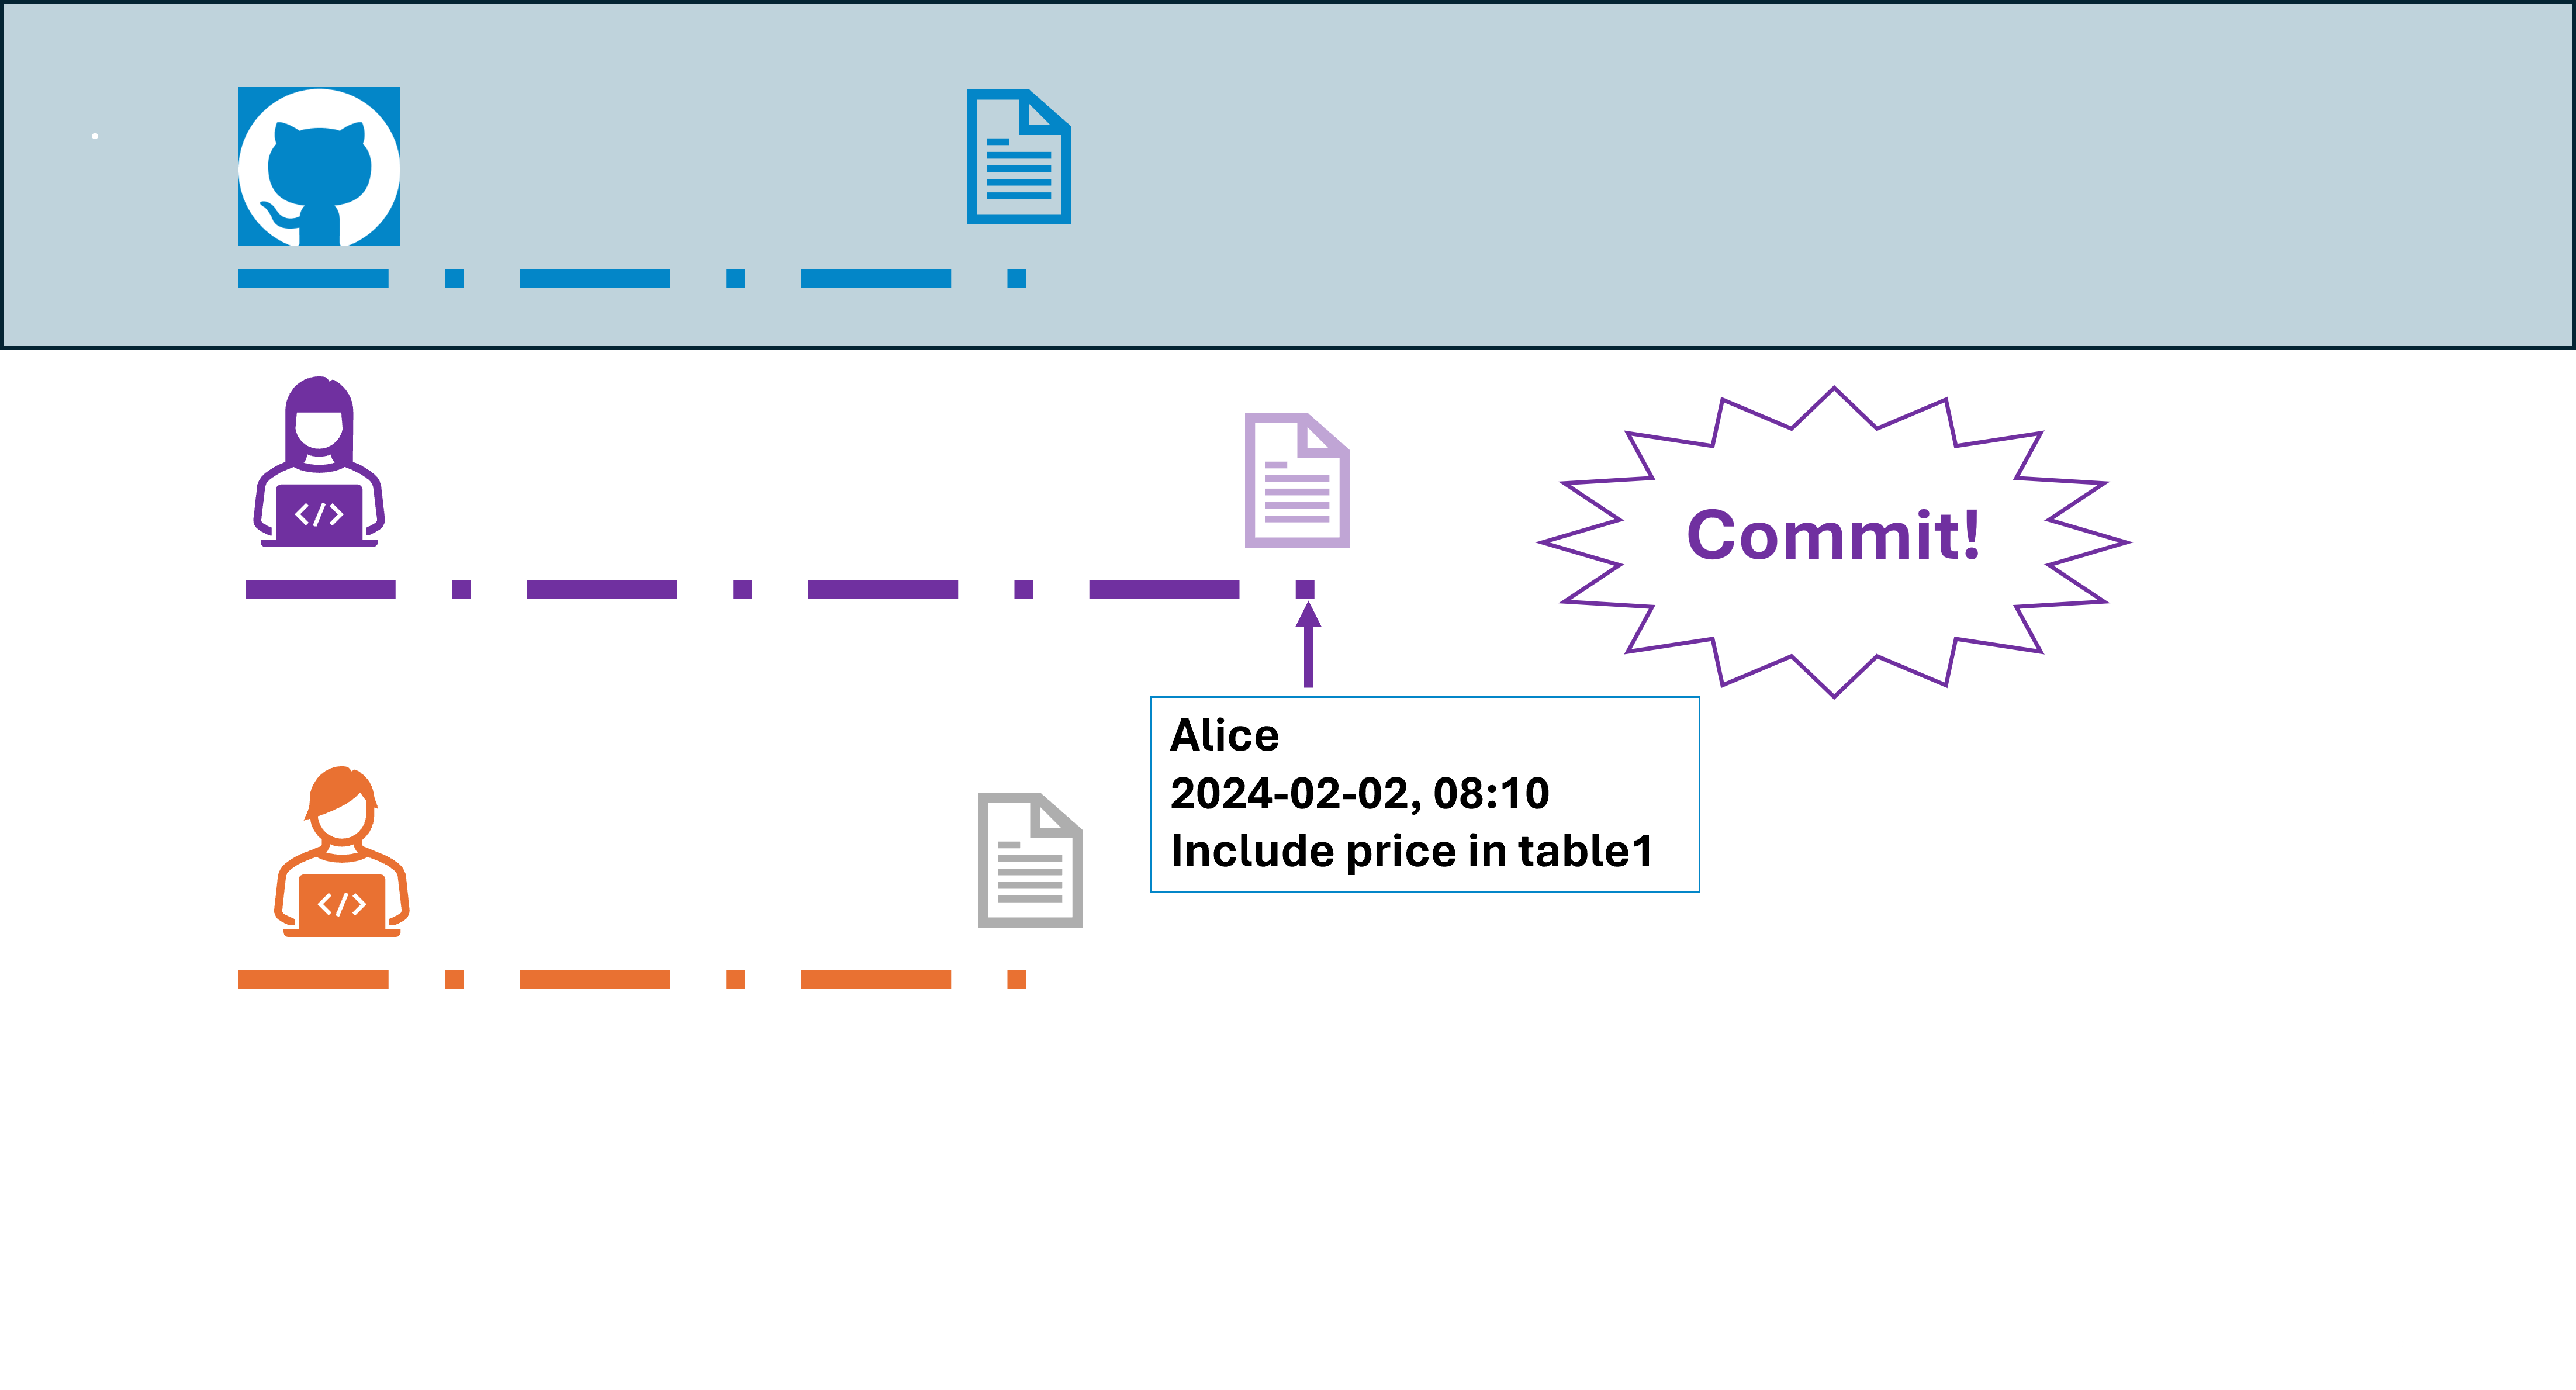
\includegraphics[width=1.1\textwidth]{GitSimple2.png} \\  }
    \only<3>{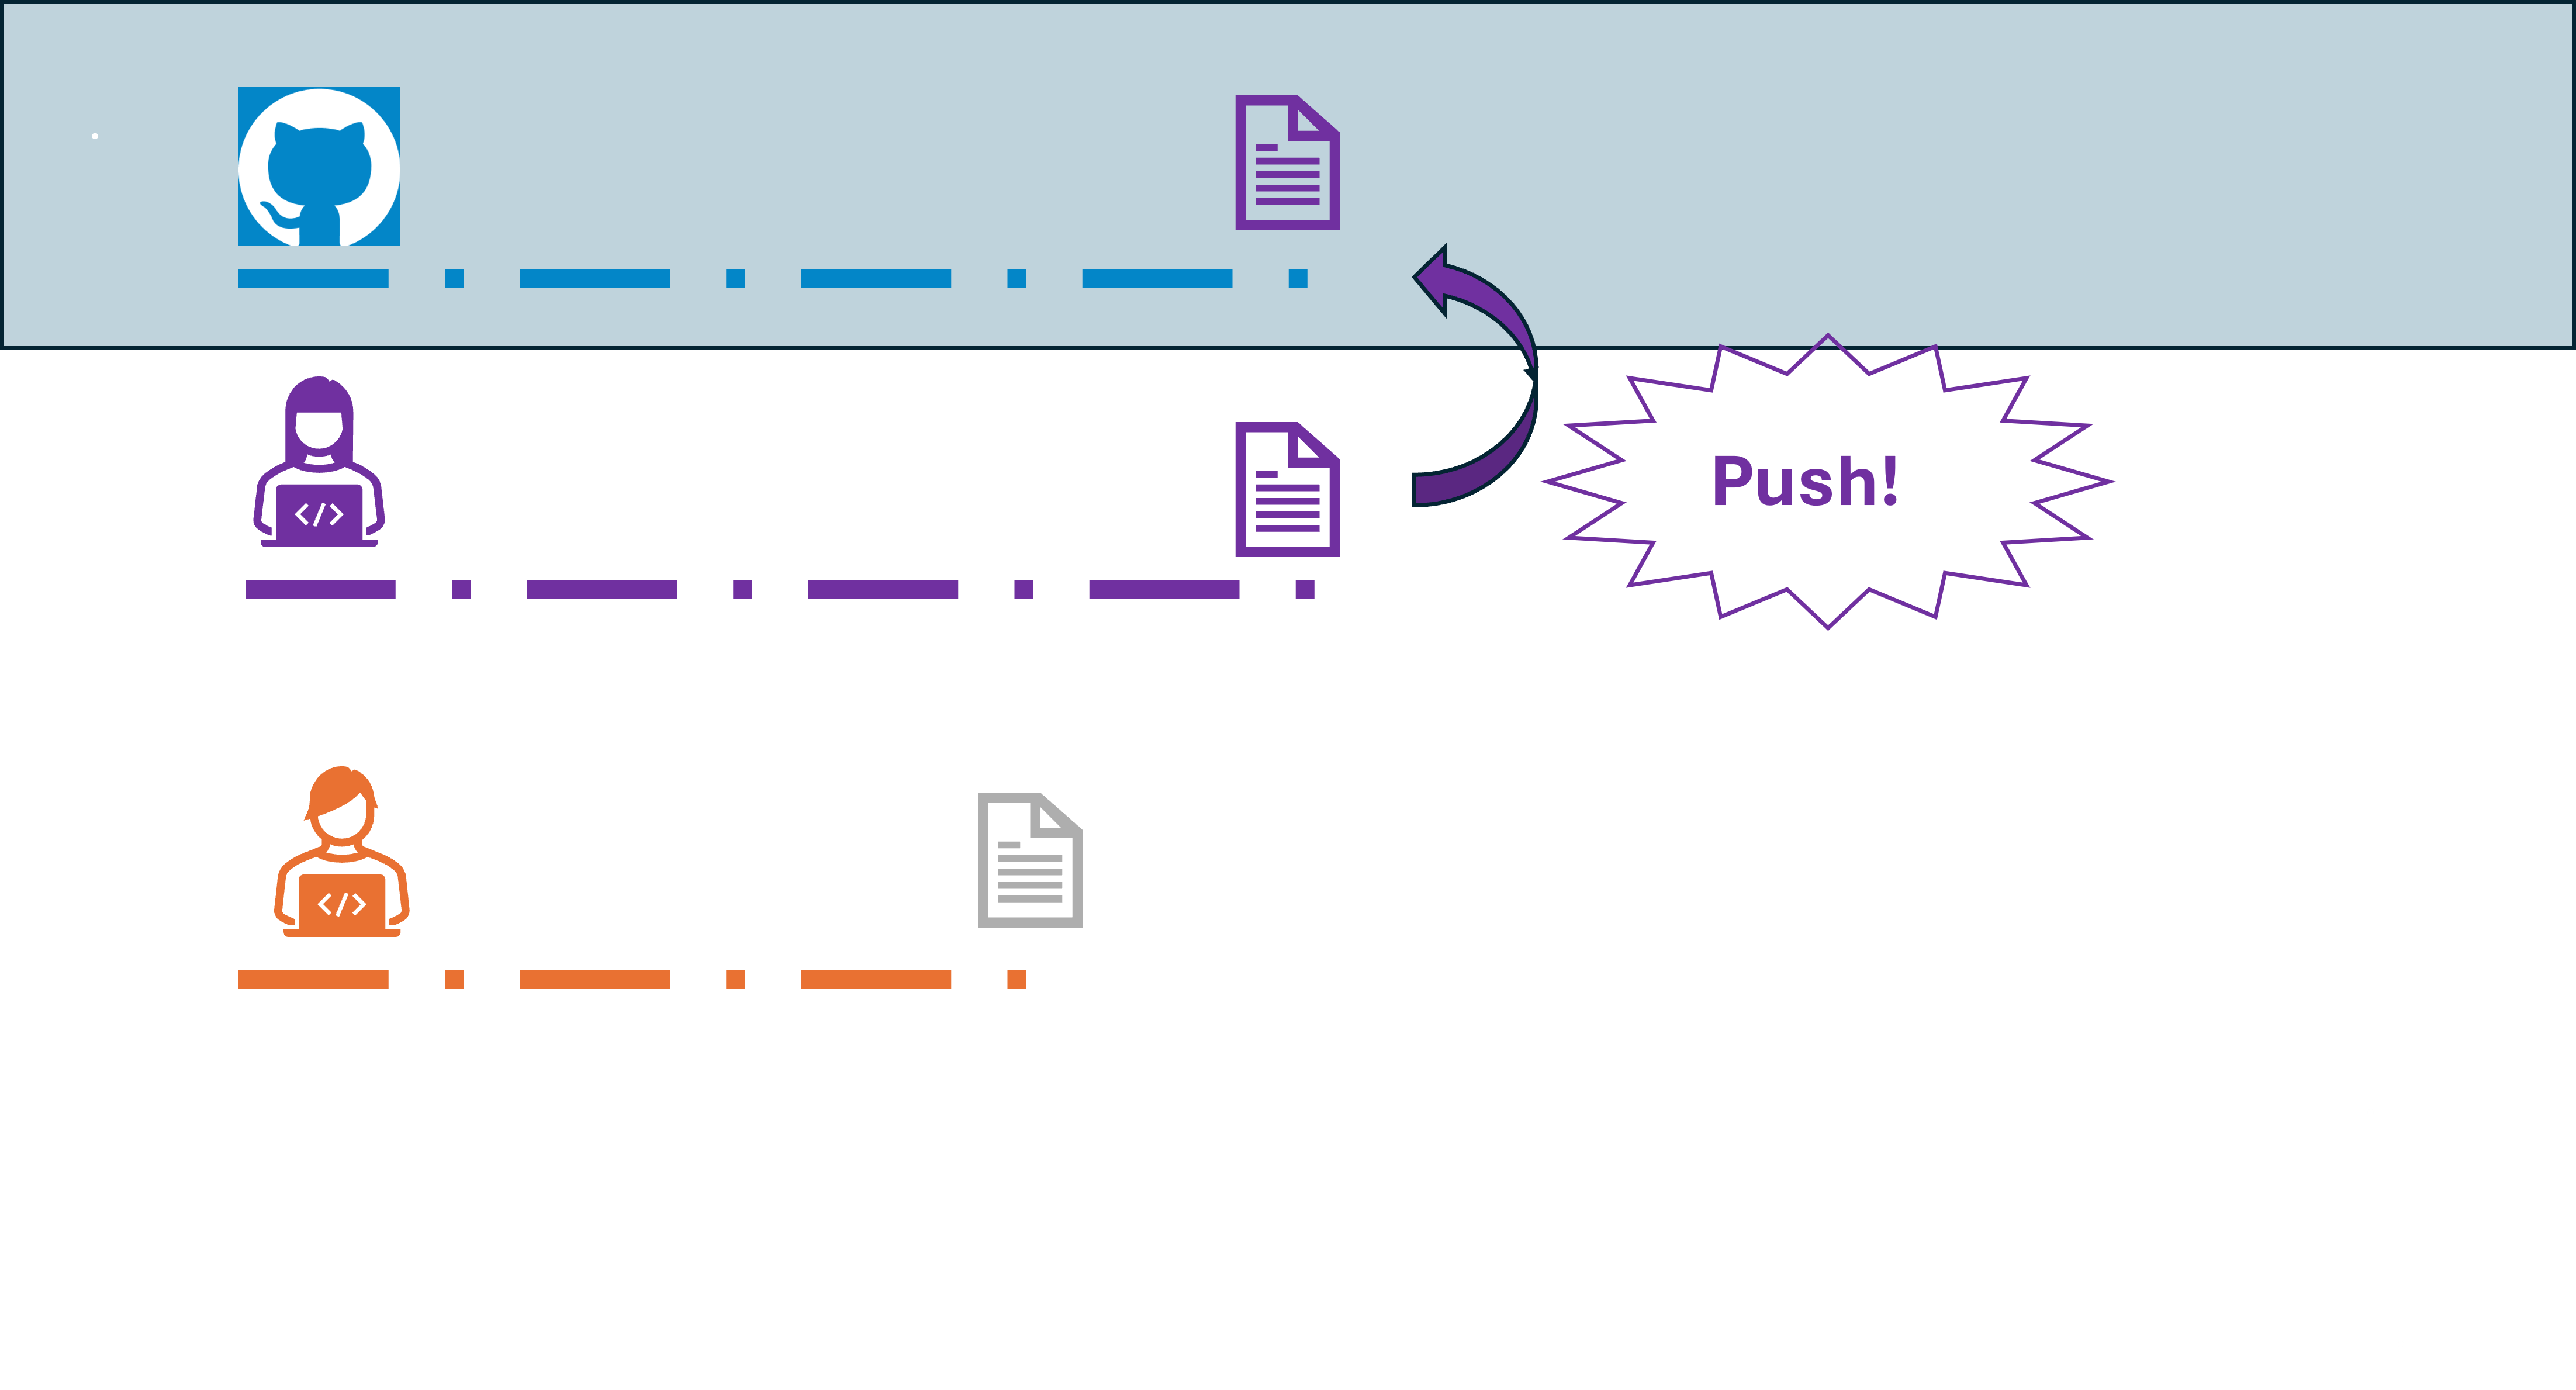
\includegraphics[width=1.1\textwidth]{GitSimple3.png} \\  }
    \only<4>{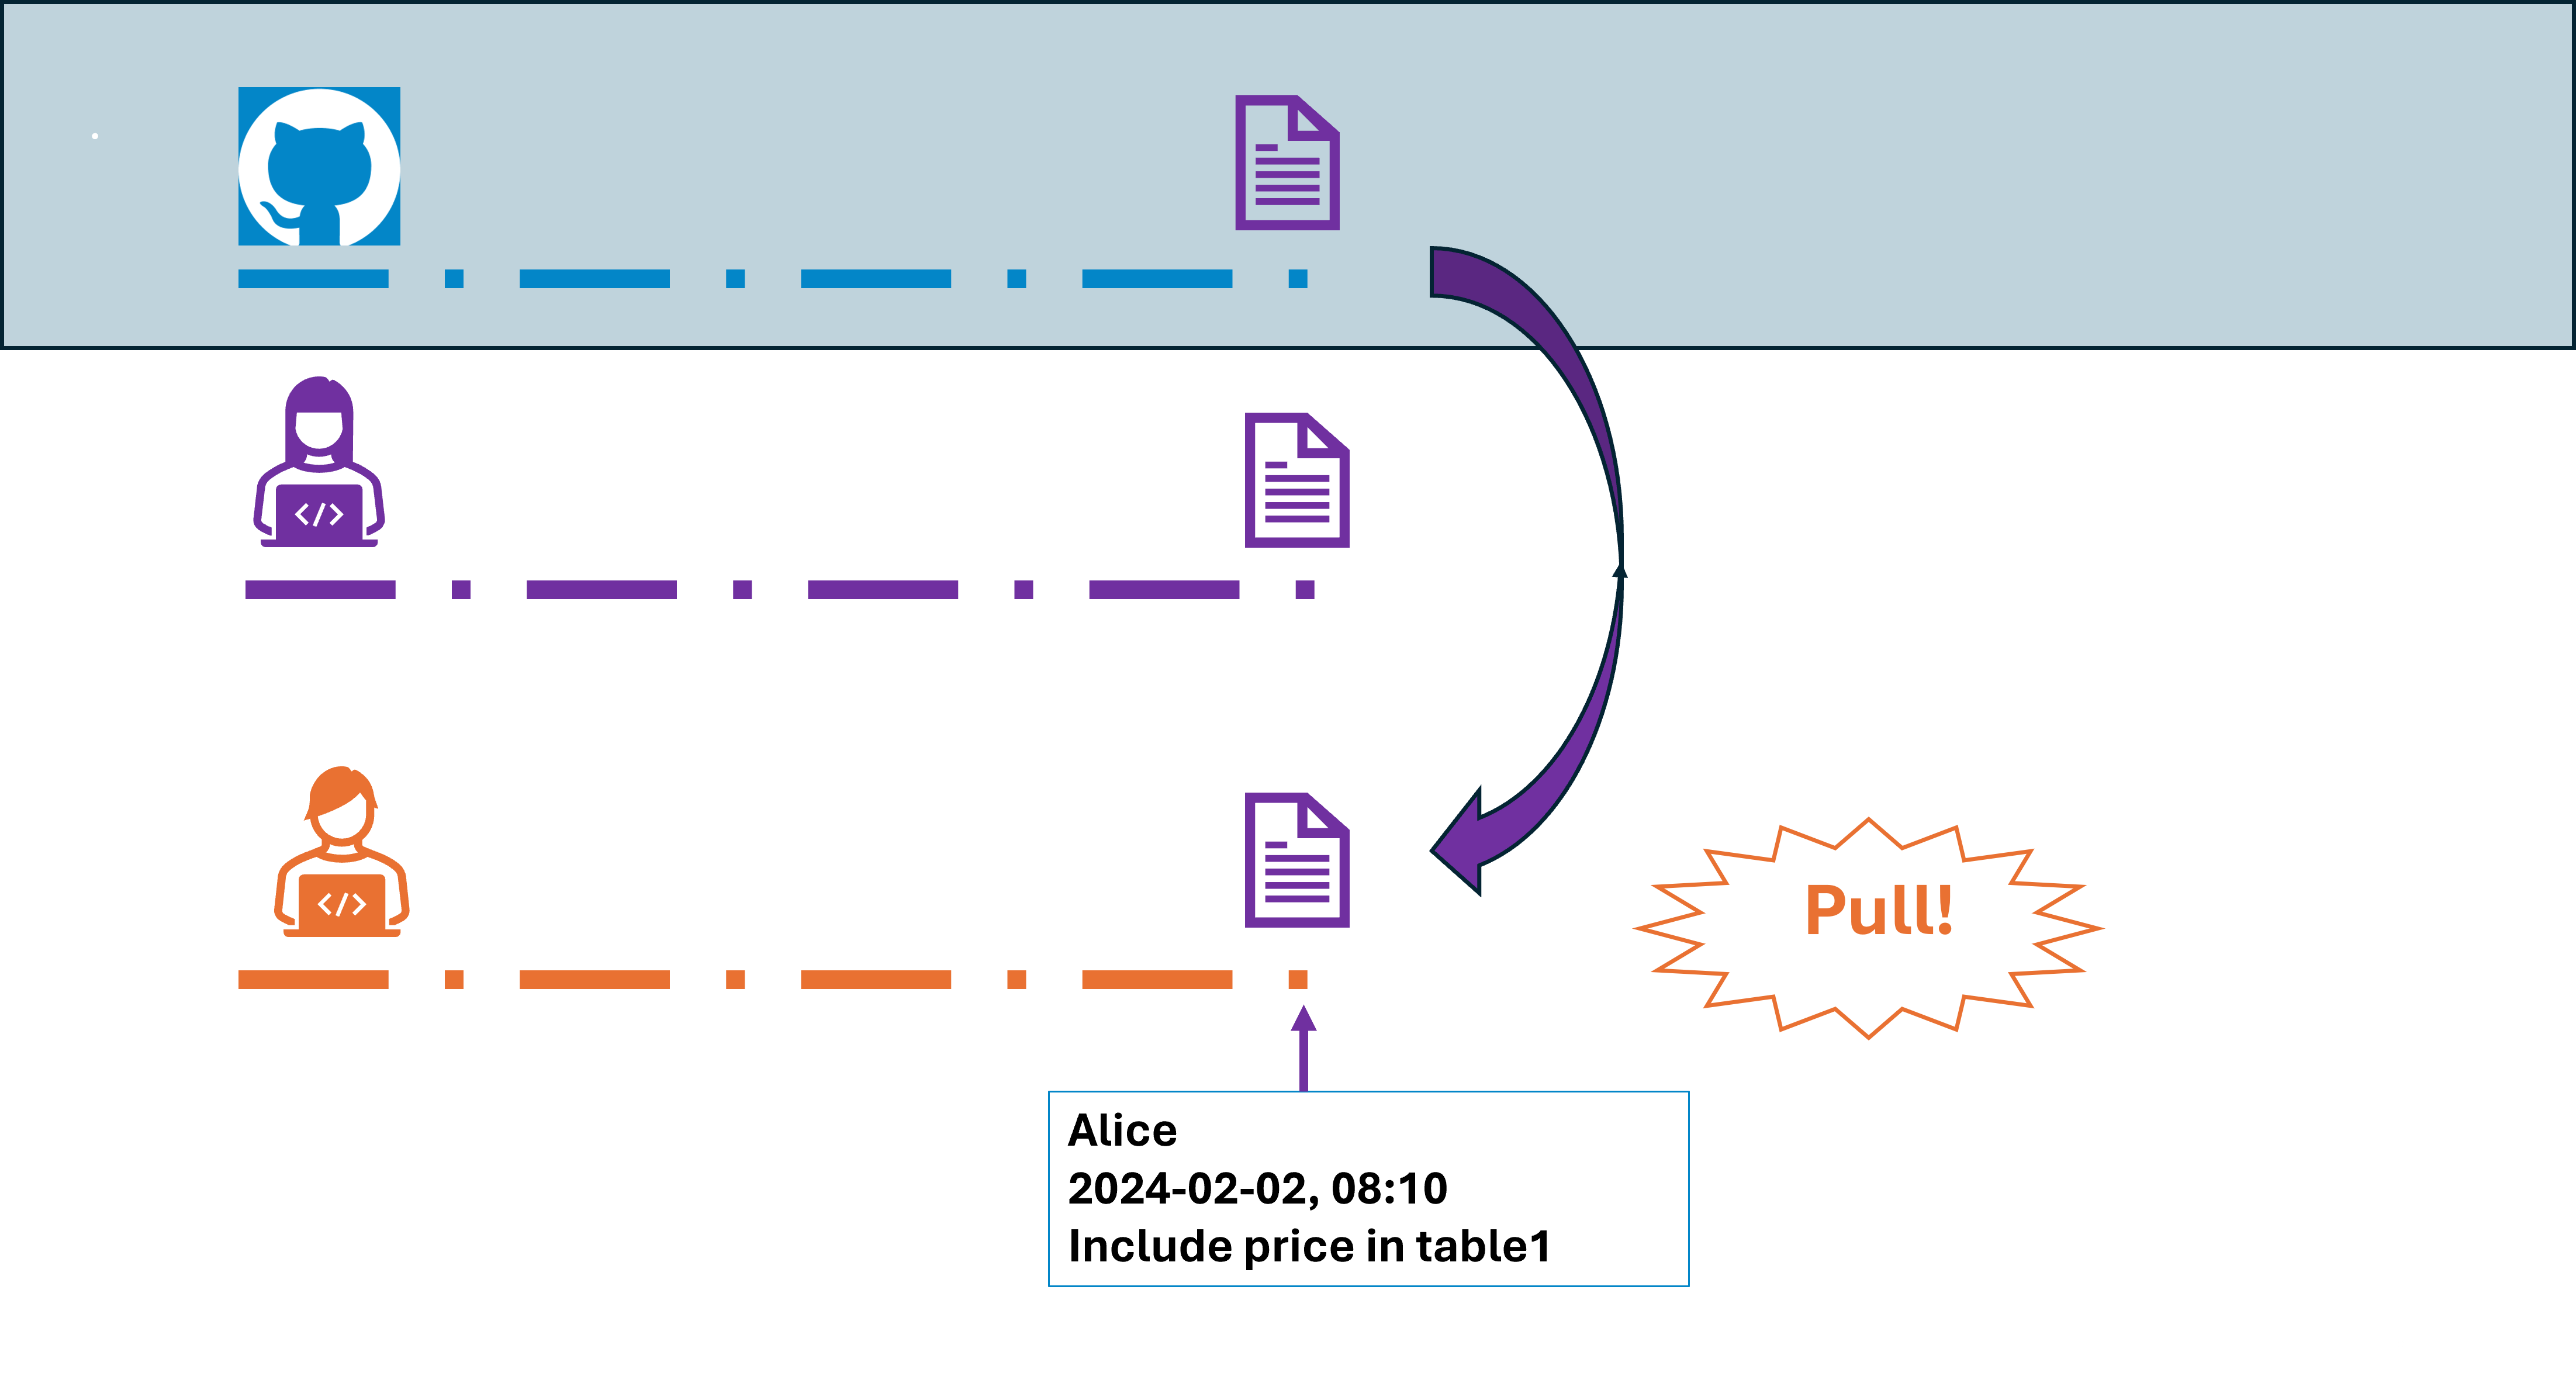
\includegraphics[width=1.1\textwidth]{GitSimple4.png}   }
\end{itemize}
\end{frame}

\begin{frame}
\frametitle{Important notions}
\begin{columns}[t]
 \begin{column}{0.5\textwidth}
    \begin{itemize}[<+->]
     \item[]
   \begin{center}
    \textcolor{brique}{\textbf{Spaces}}
   \end{center}
    \item  \textcolor{siap}{\textbf{Local working directory:}}
    \item[$\hookrightarrow$] Folder with your file(s)
    \item  \textcolor{siap}{\textbf{Staging area:}}
    \item[$\hookrightarrow$] Local "space" where modified file(s) are stored before commit
    \item \textcolor{siap}{\textbf{Remote repository:}}
    \item[$\hookrightarrow$] Folder  on GitHub platform
    \end{itemize}
 \end{column}
 \begin{column}{0.5\textwidth}
    \begin{itemize}[<+->]
        \item[]
        \begin{center}
        \textcolor{brique}{\textbf{Actions}}
        \end{center}
        \item \textcolor{siap}{\textbf{Commit:}}
        \item[$\hookrightarrow$] A snapshot of file changes
        \item \textcolor{siap}{\textbf{Commit message:}}
        \item[$\hookrightarrow$] A concise description of the changes made
        \item \textcolor{siap}{\textbf{Push:}}
        \item[$\hookrightarrow$] Action of sending modified file(s) to GitHub
        \item \textcolor{siap}{\textbf{Pull:}}
        \item[$\hookrightarrow$] Action of retrieving modified file(s) to local working directory


    \end{itemize}
 \end{column}
\end{columns}
\end{frame}

\begin{frame}
\frametitle{Git for collaborating:  Details}
\textcolor{violet}{\textbf{Alice}} and \textcolor{orange}{\textbf{Bob}} work on the same file (Details)
\pause

\begin{itemize}
\item[]
\only<1>{
\includegraphics[width=1.0\textwidth]{GitPrinciple1.png} \\ }
\only<2>{
\includegraphics[width=1.0\textwidth]{GitPrinciple2.png} \\ }
\only<3>{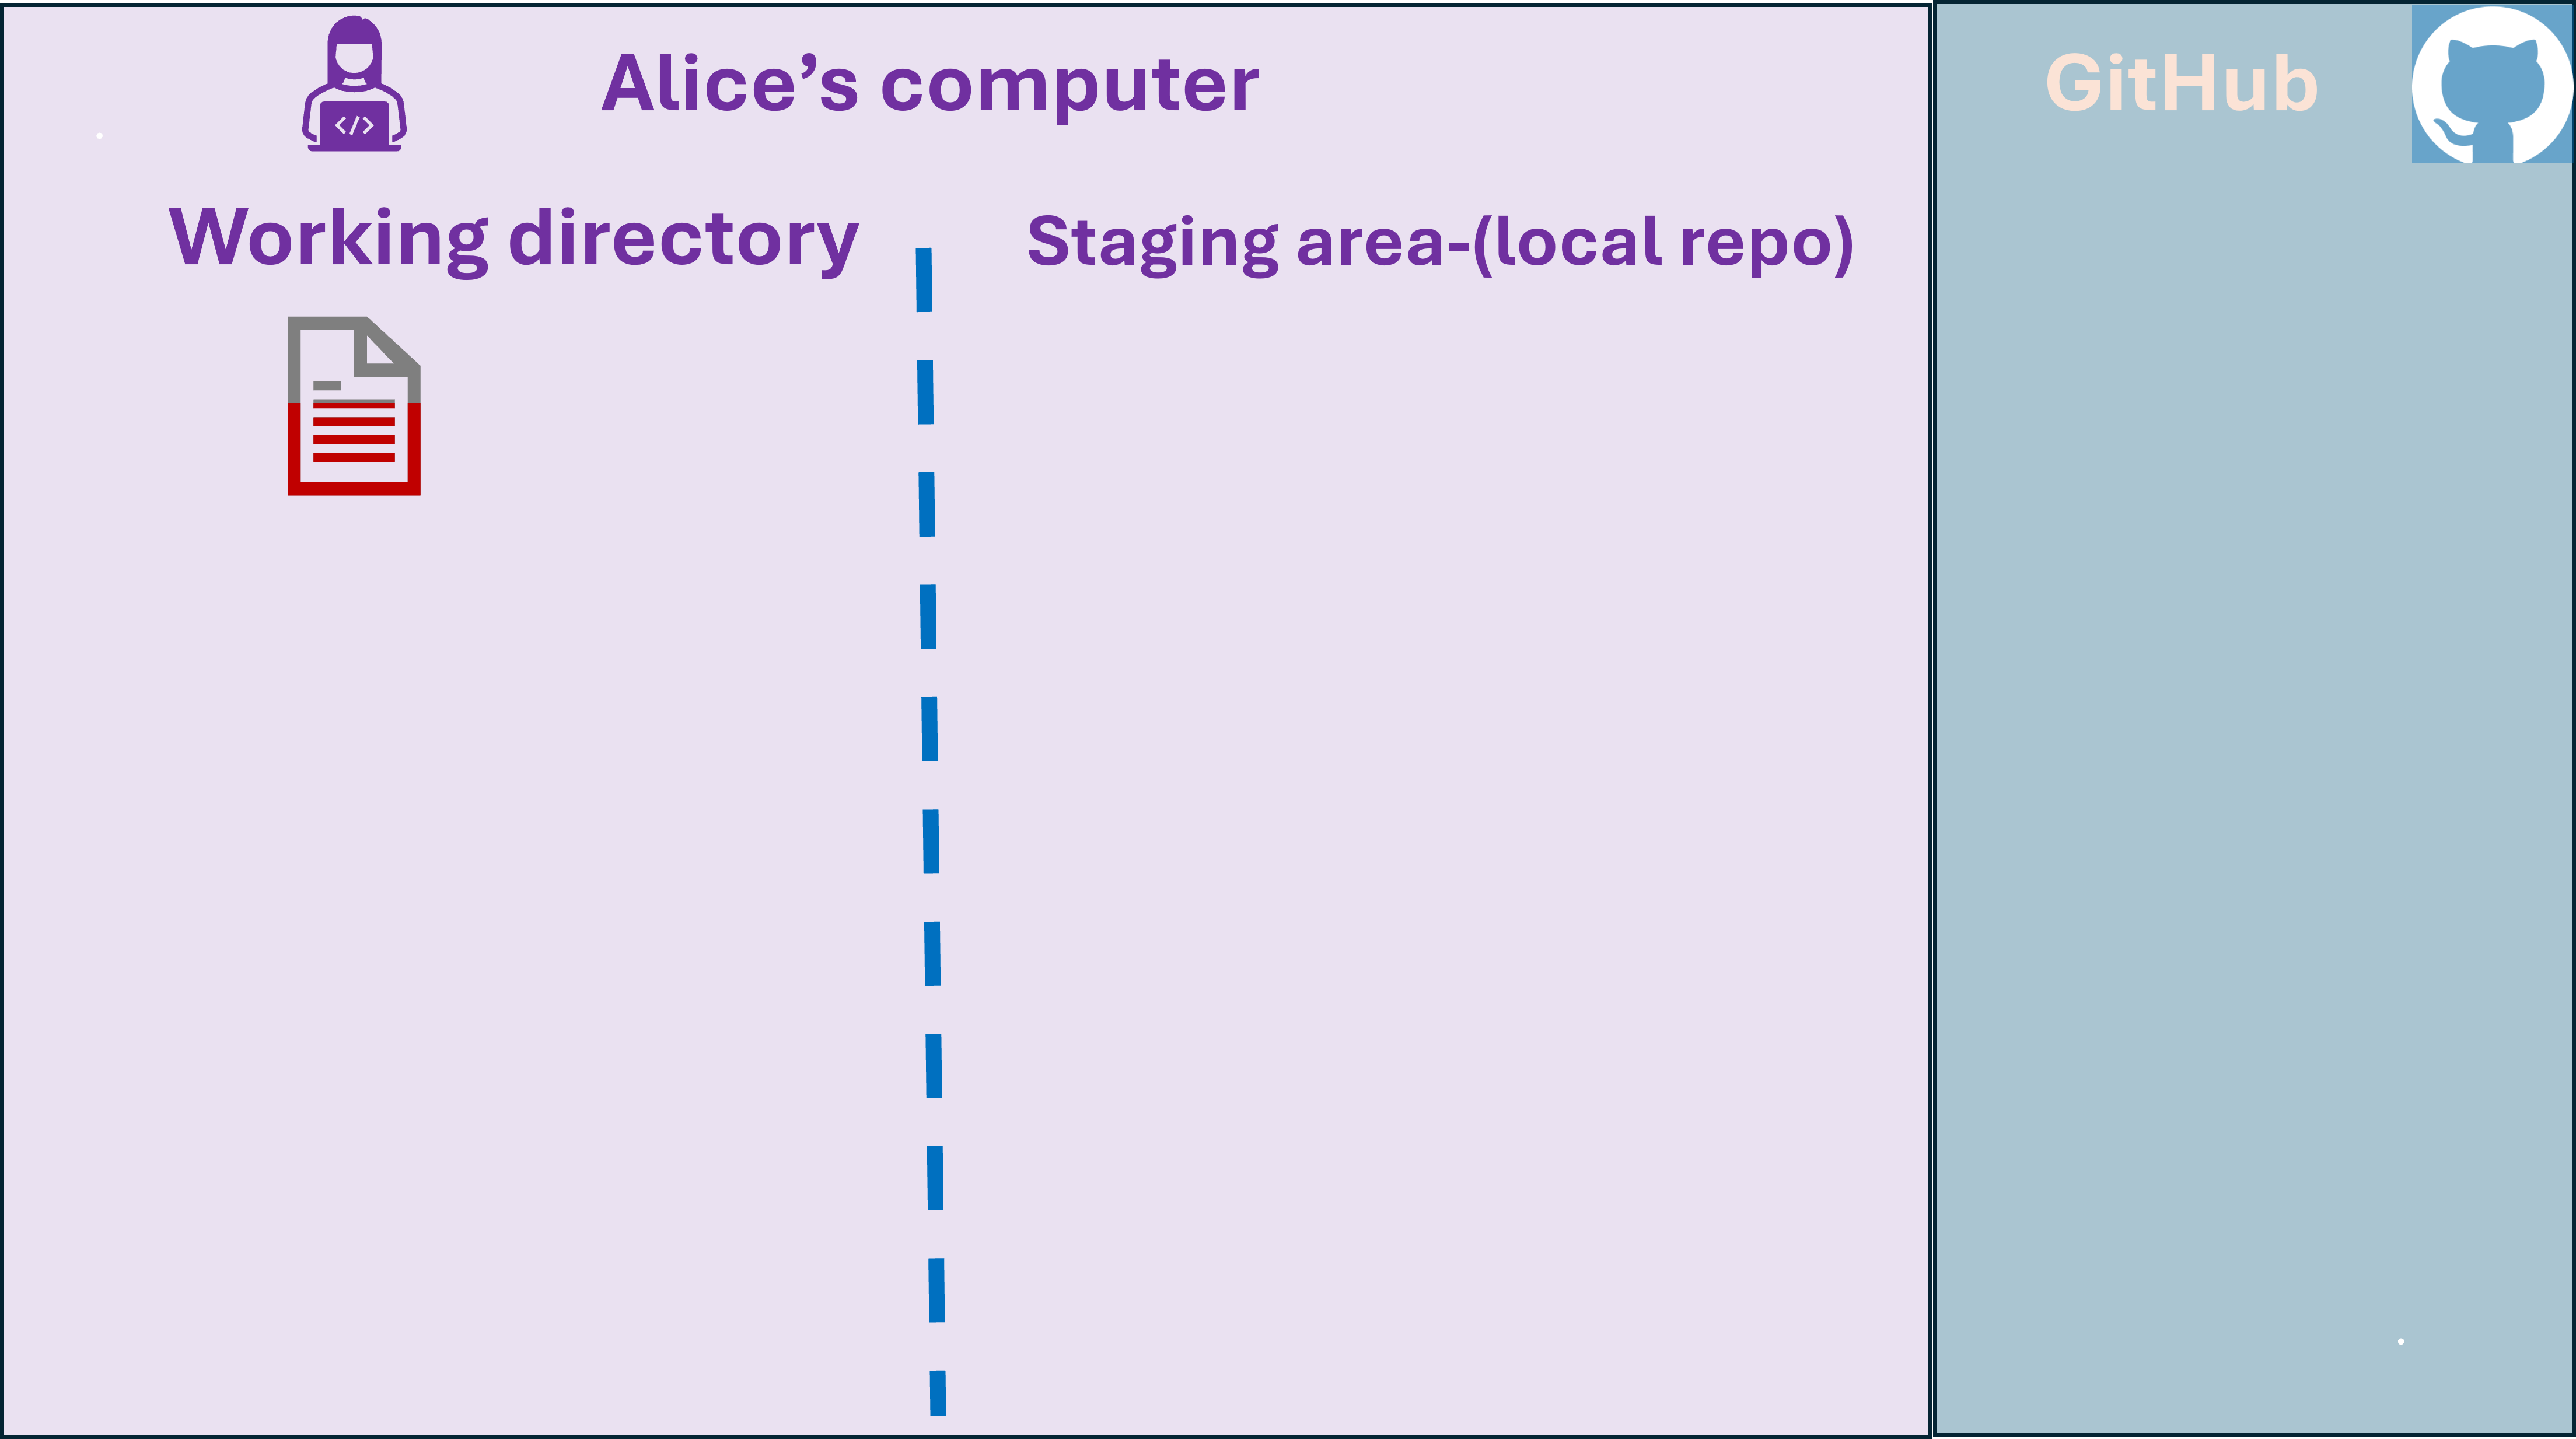
\includegraphics[width=1.0\textwidth]{GitPrinciple3N.png} \\ }
\only<4>{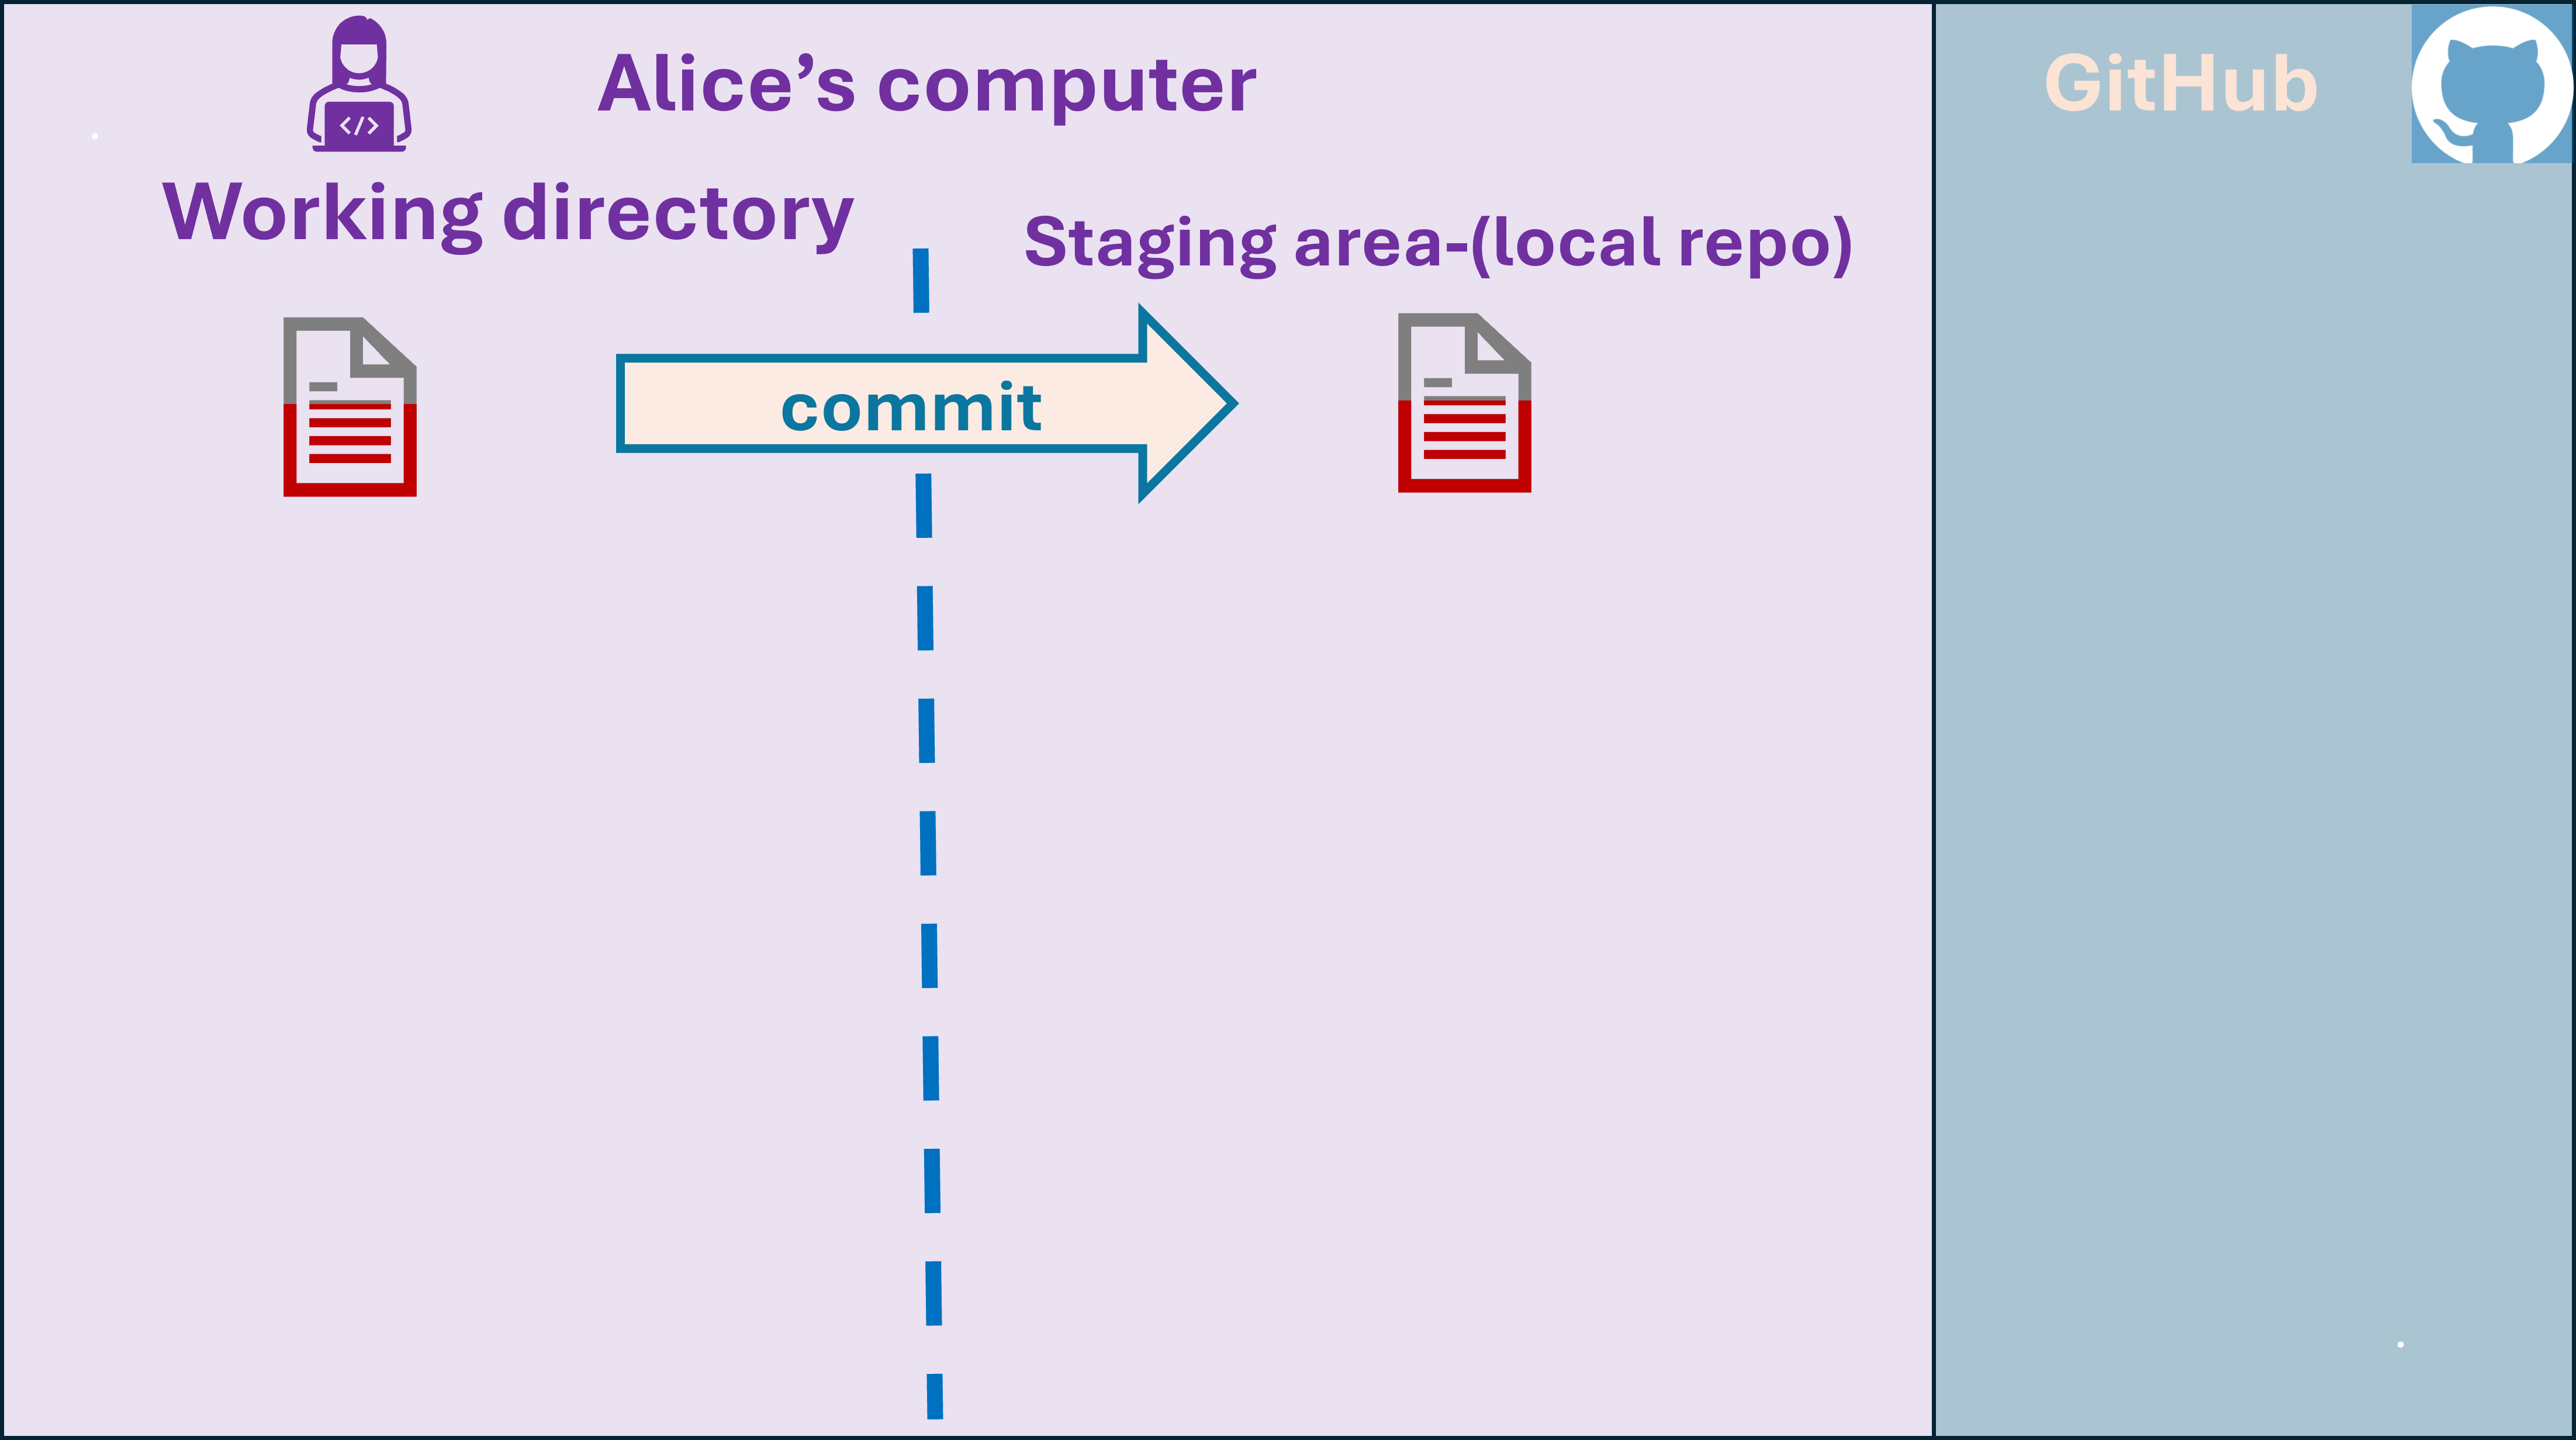
\includegraphics[width=1.0\textwidth]{GitPrinciple4N.png} \\ }
\only<5>{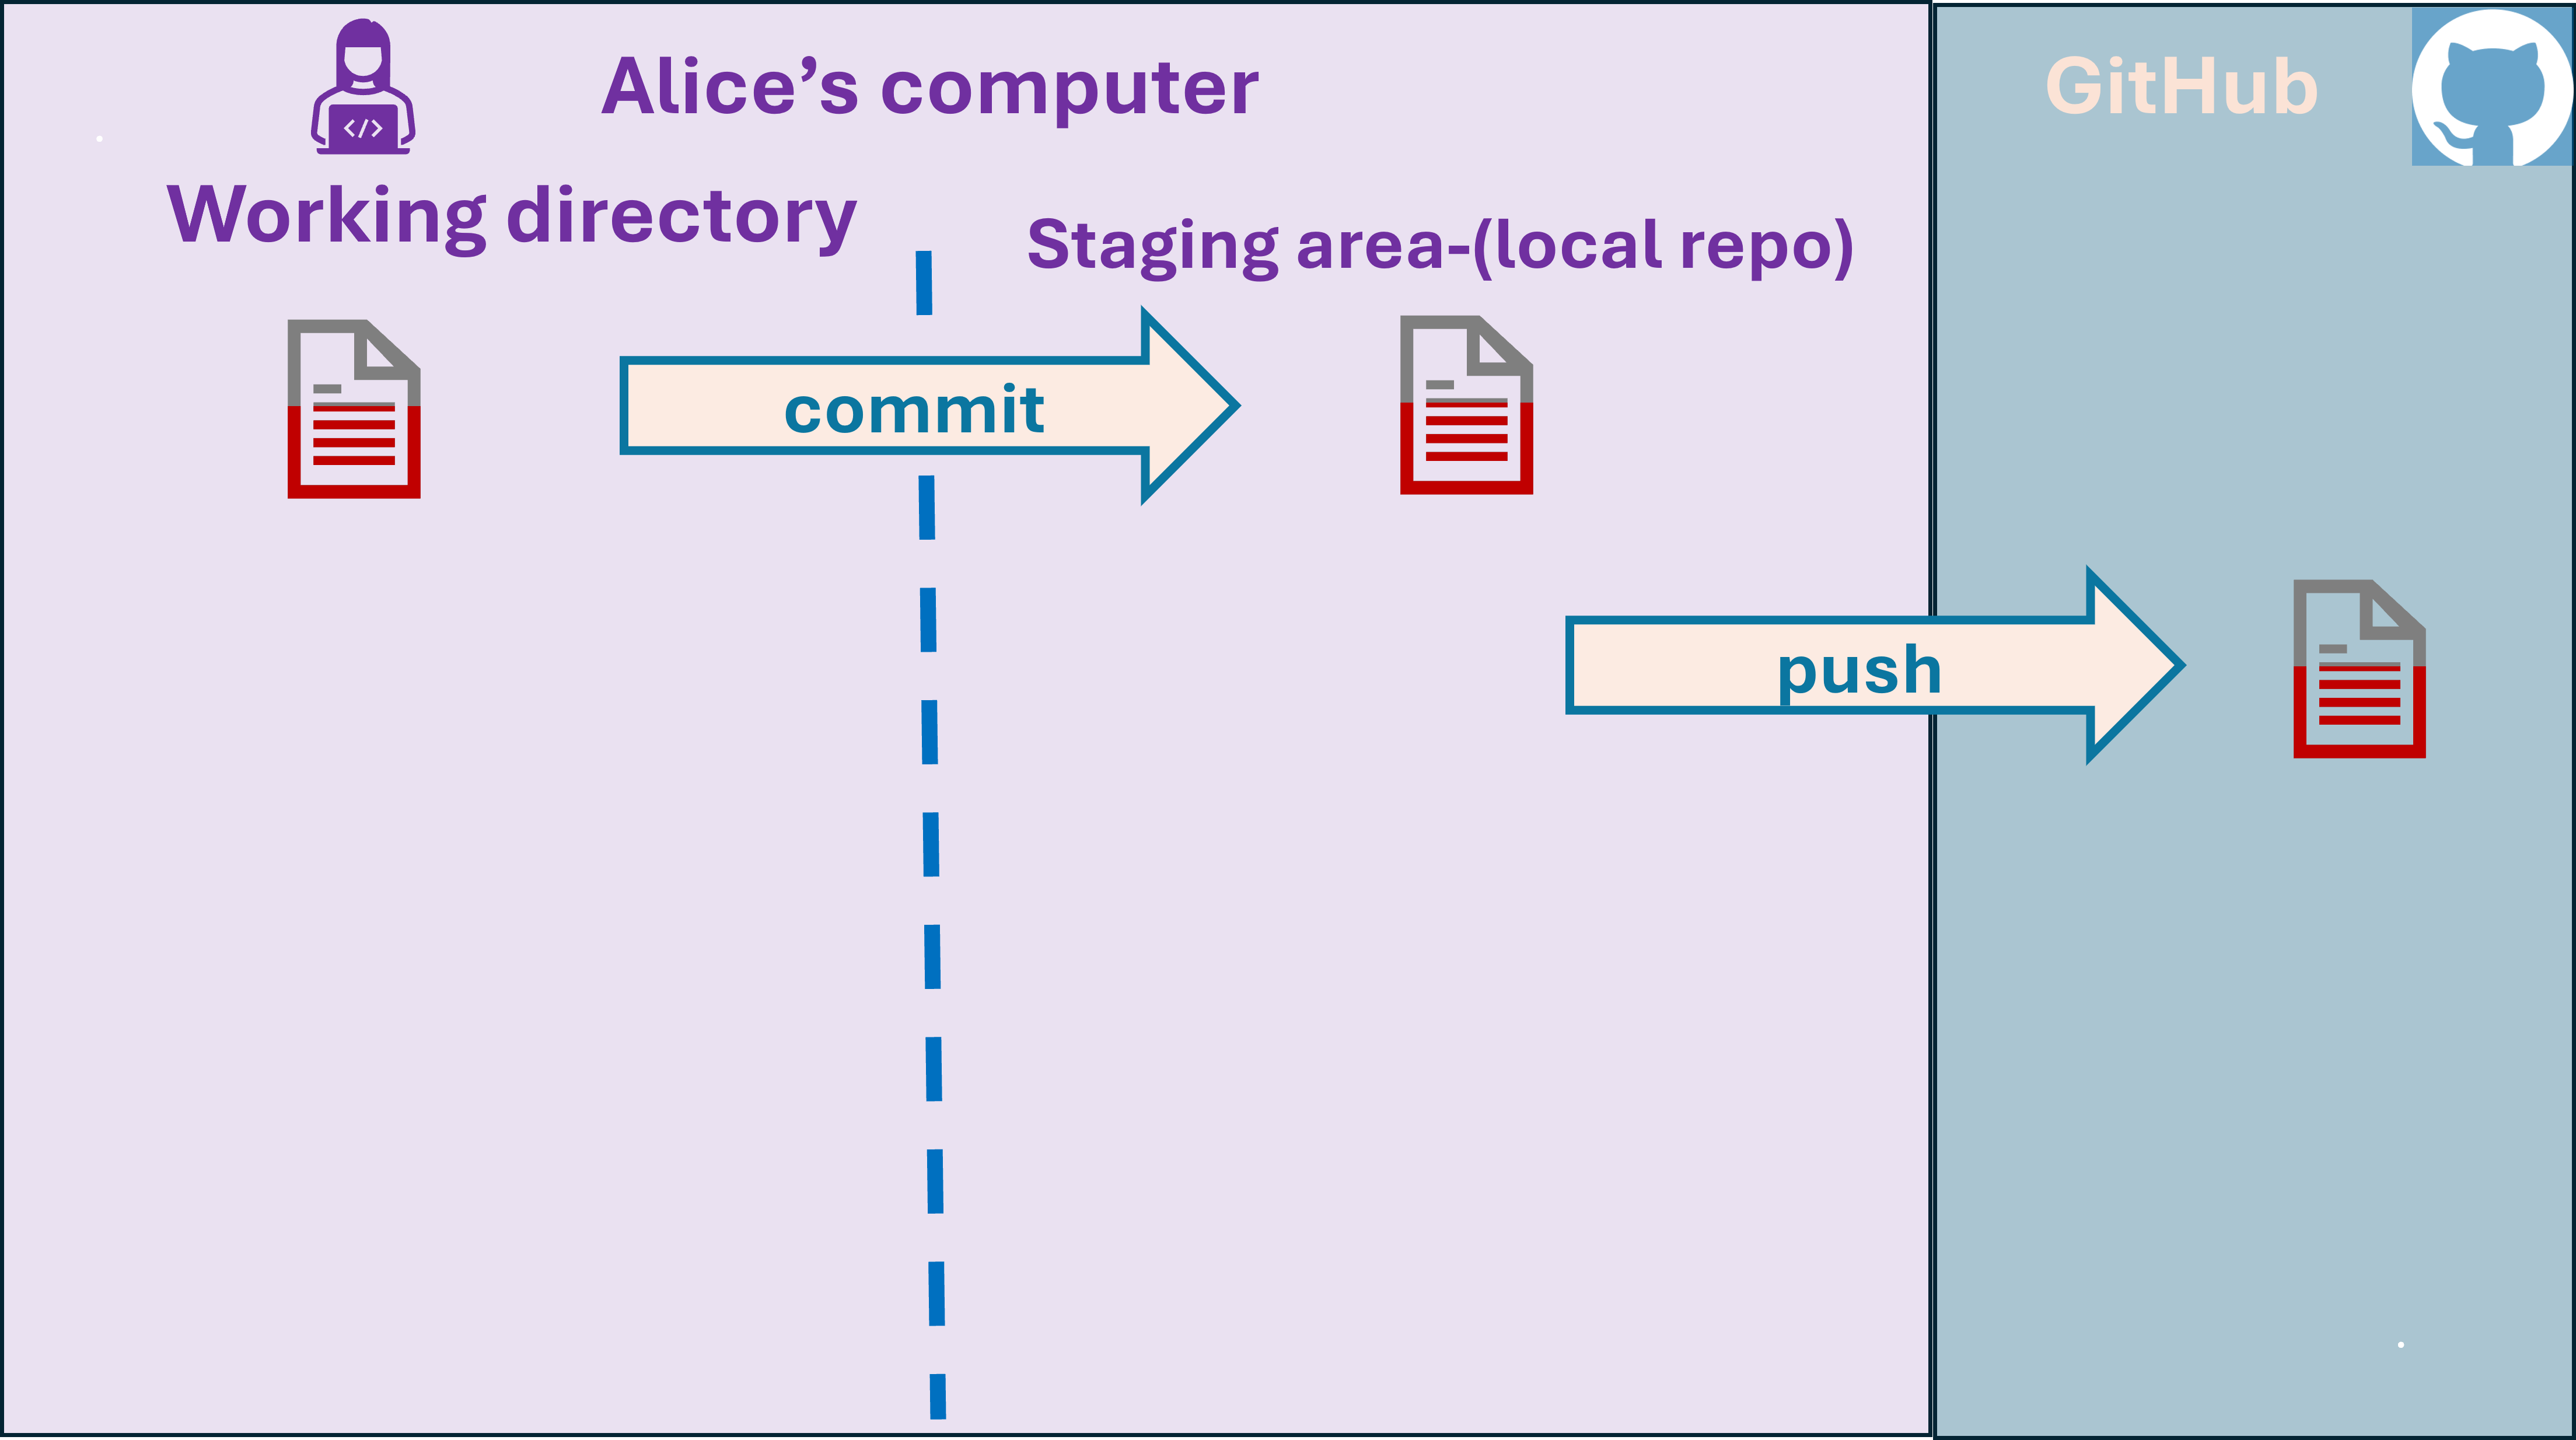
\includegraphics[width=1.0\textwidth]{GitPrinciple5N.png} \\ }
\only<6>{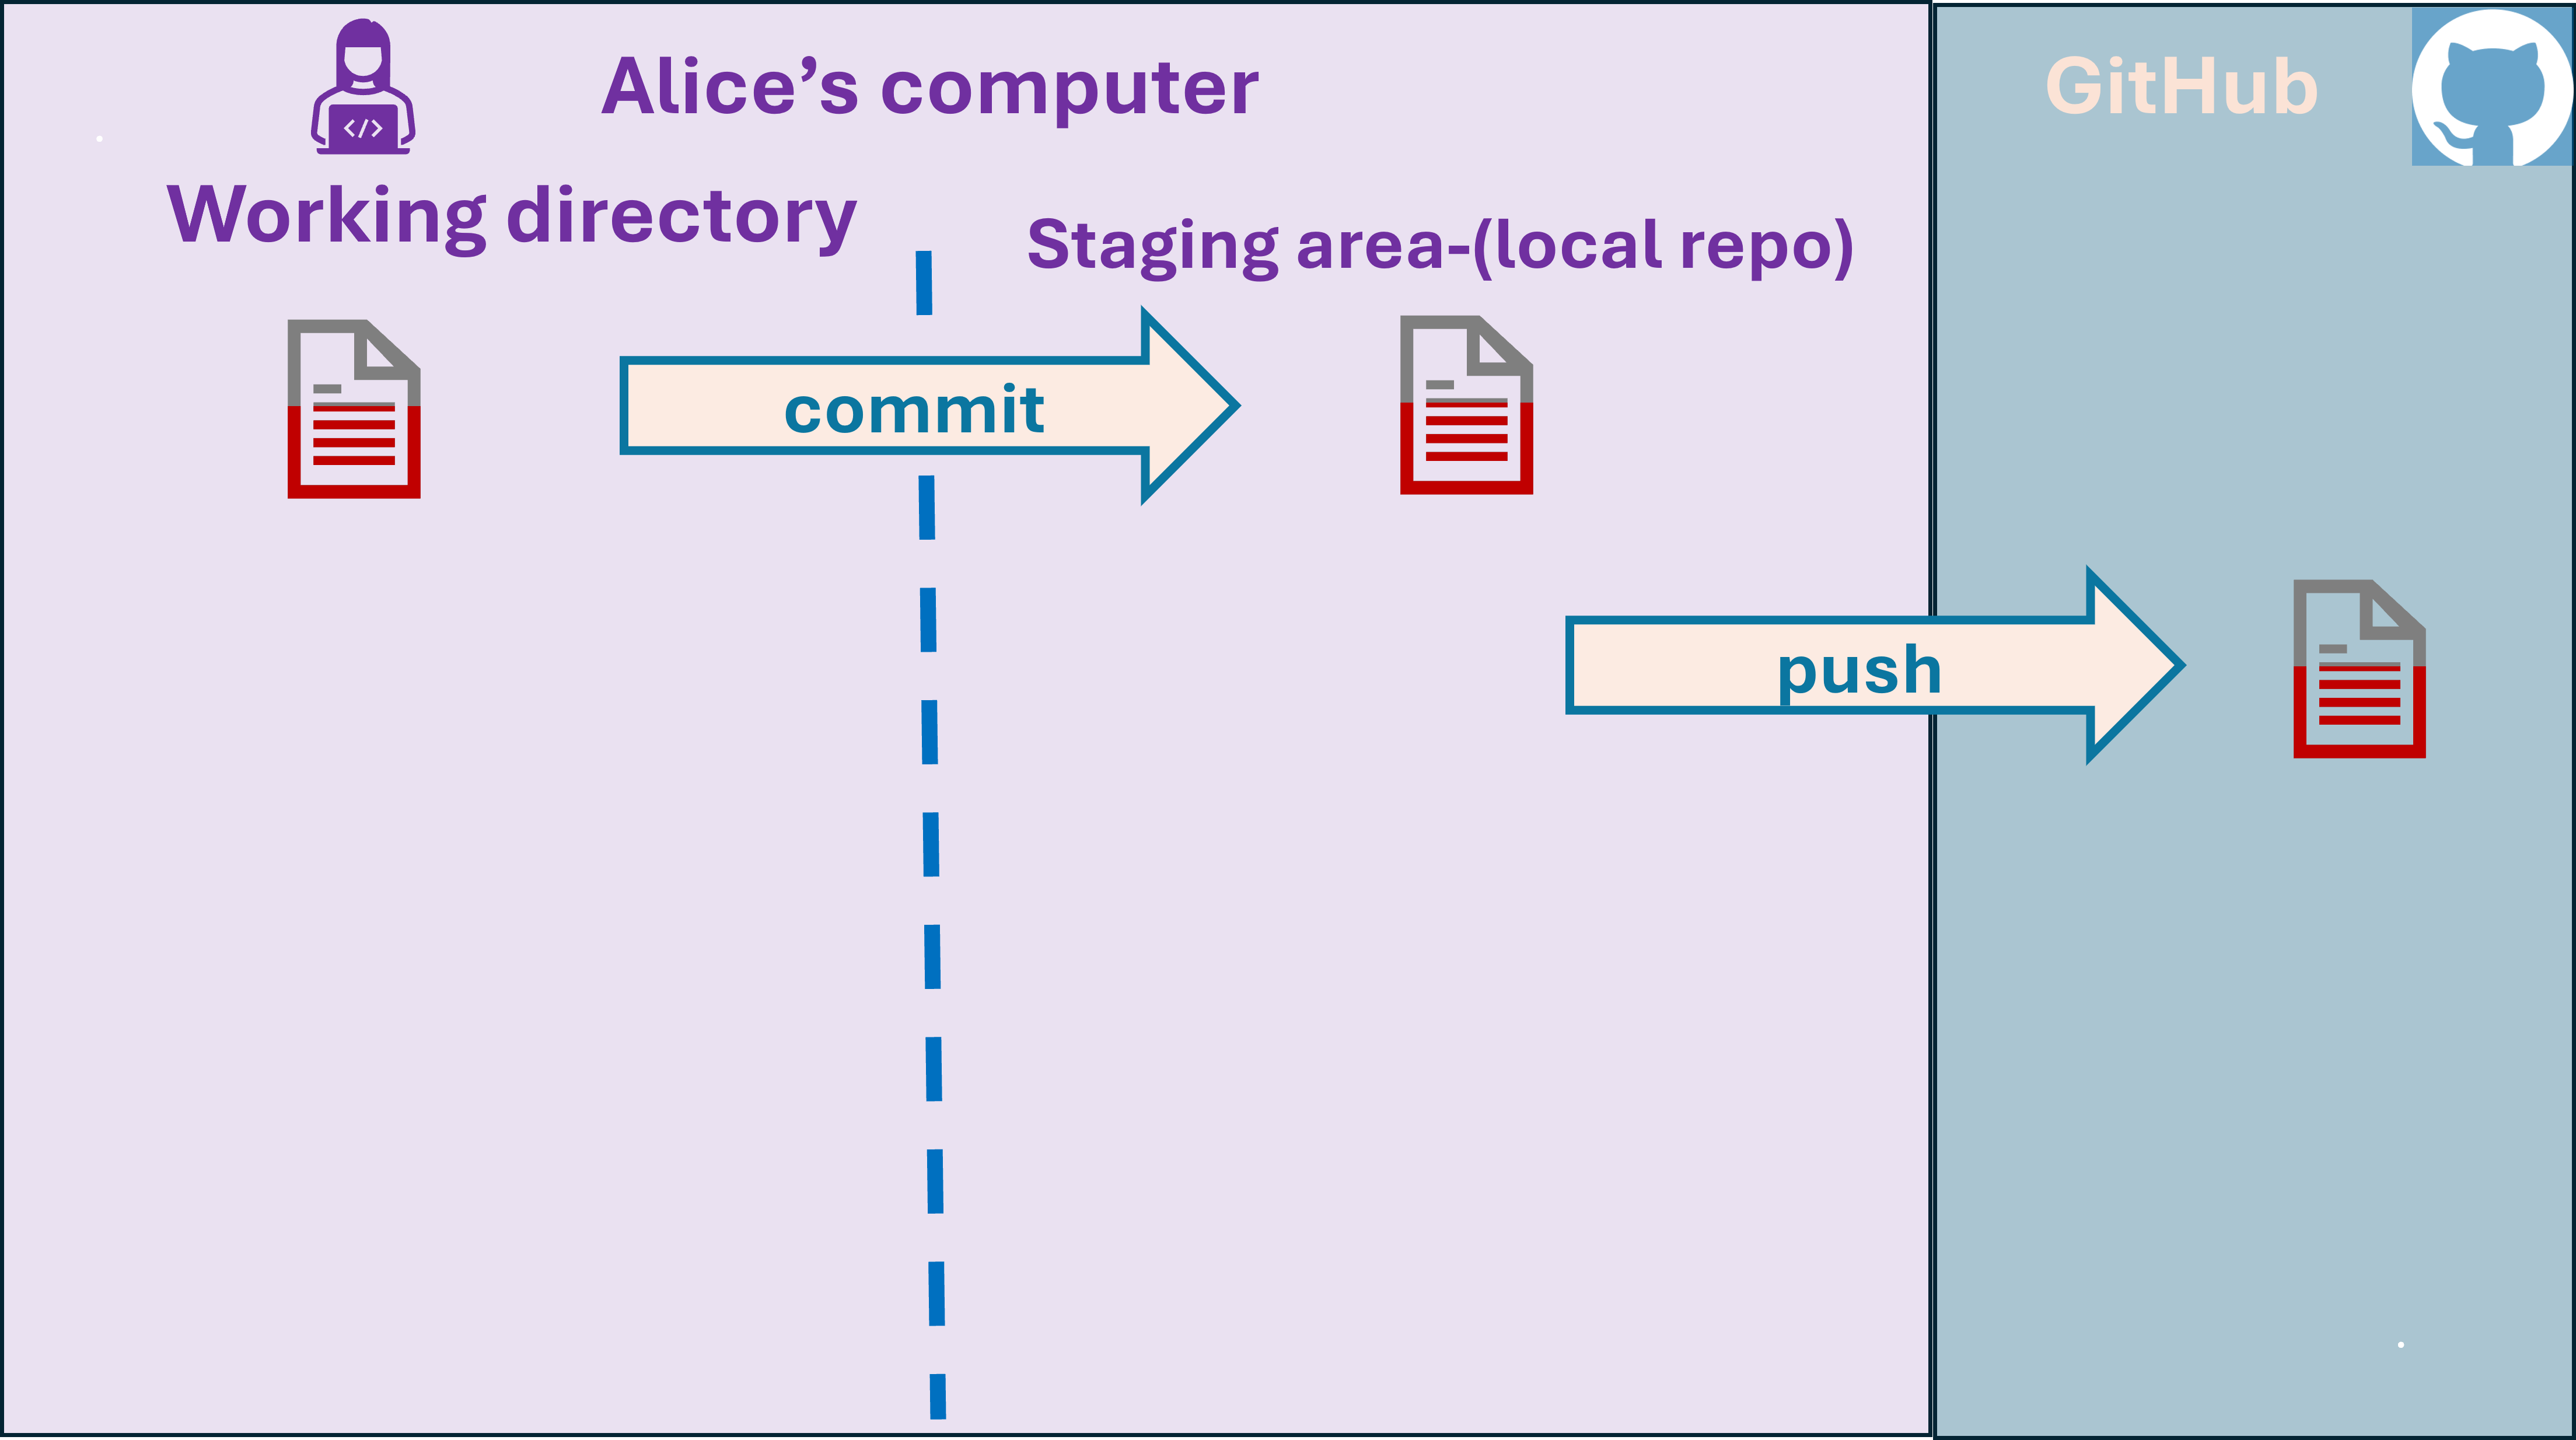
\includegraphics[width=1.0\textwidth]{GitPrinciple5N.png} \\ }
\only<7>{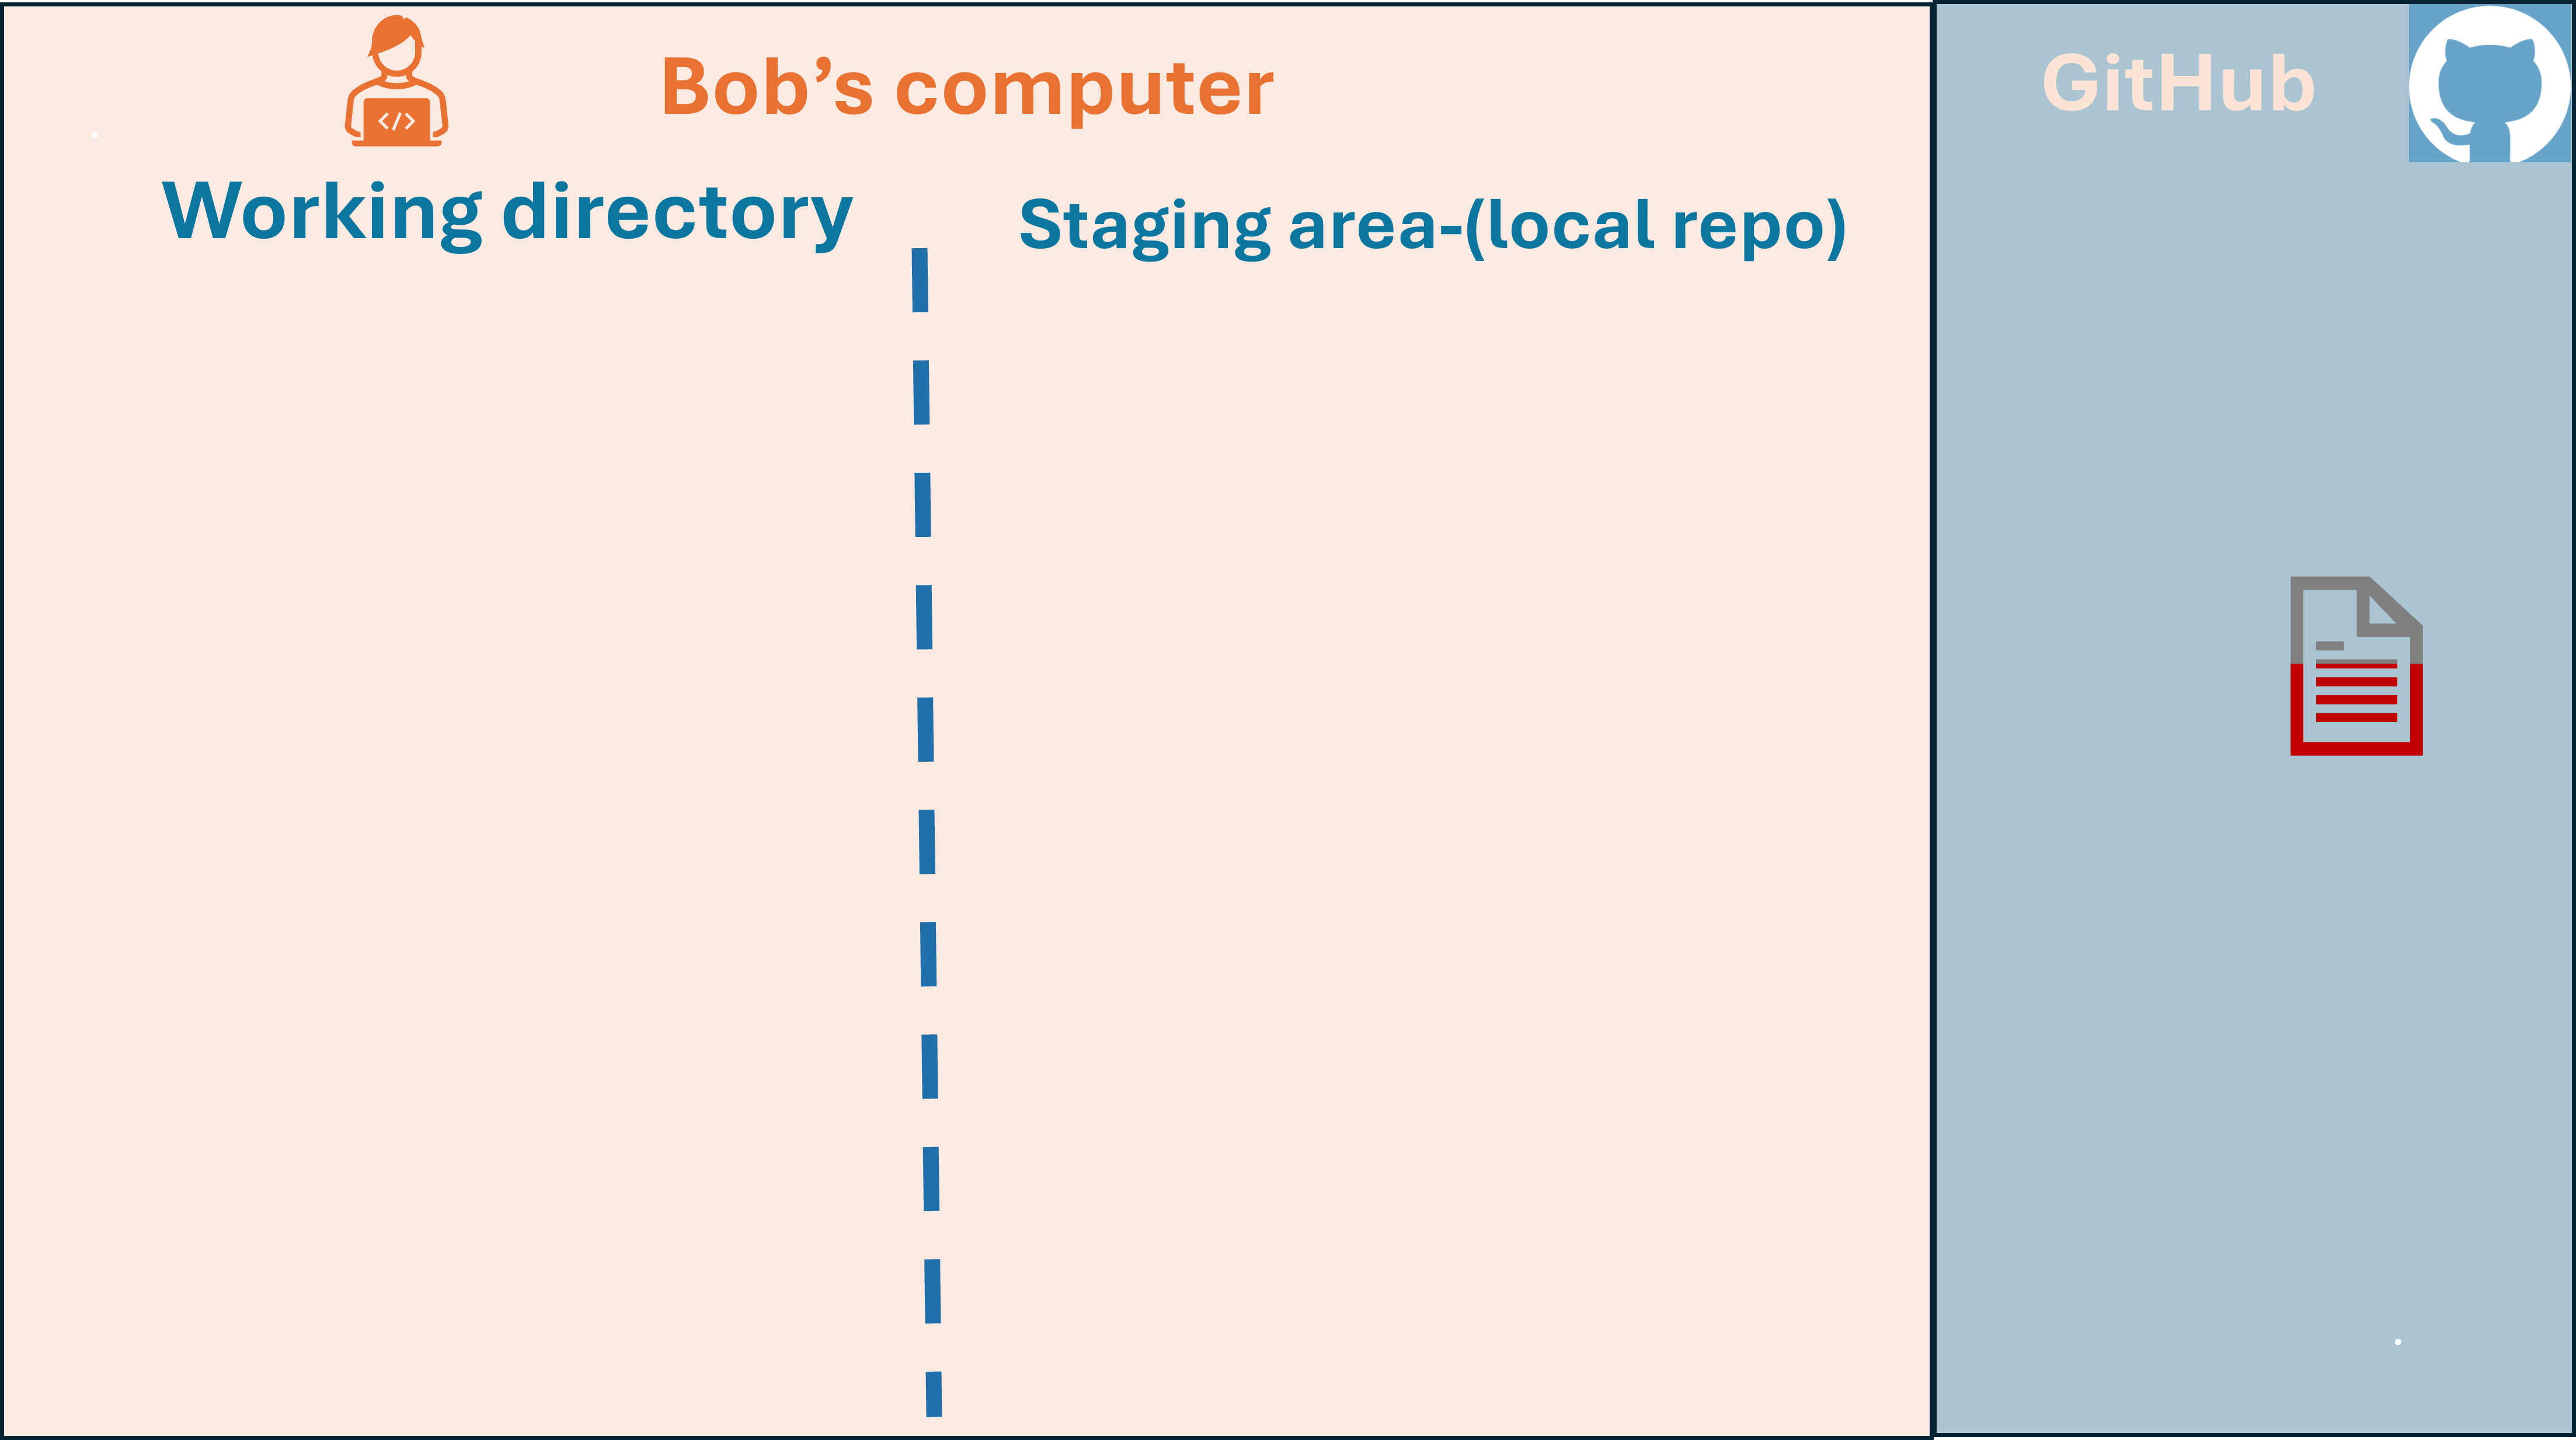
\includegraphics[width=1.0\textwidth]{GitPrinciple7N.png} \\ }
\only<8>{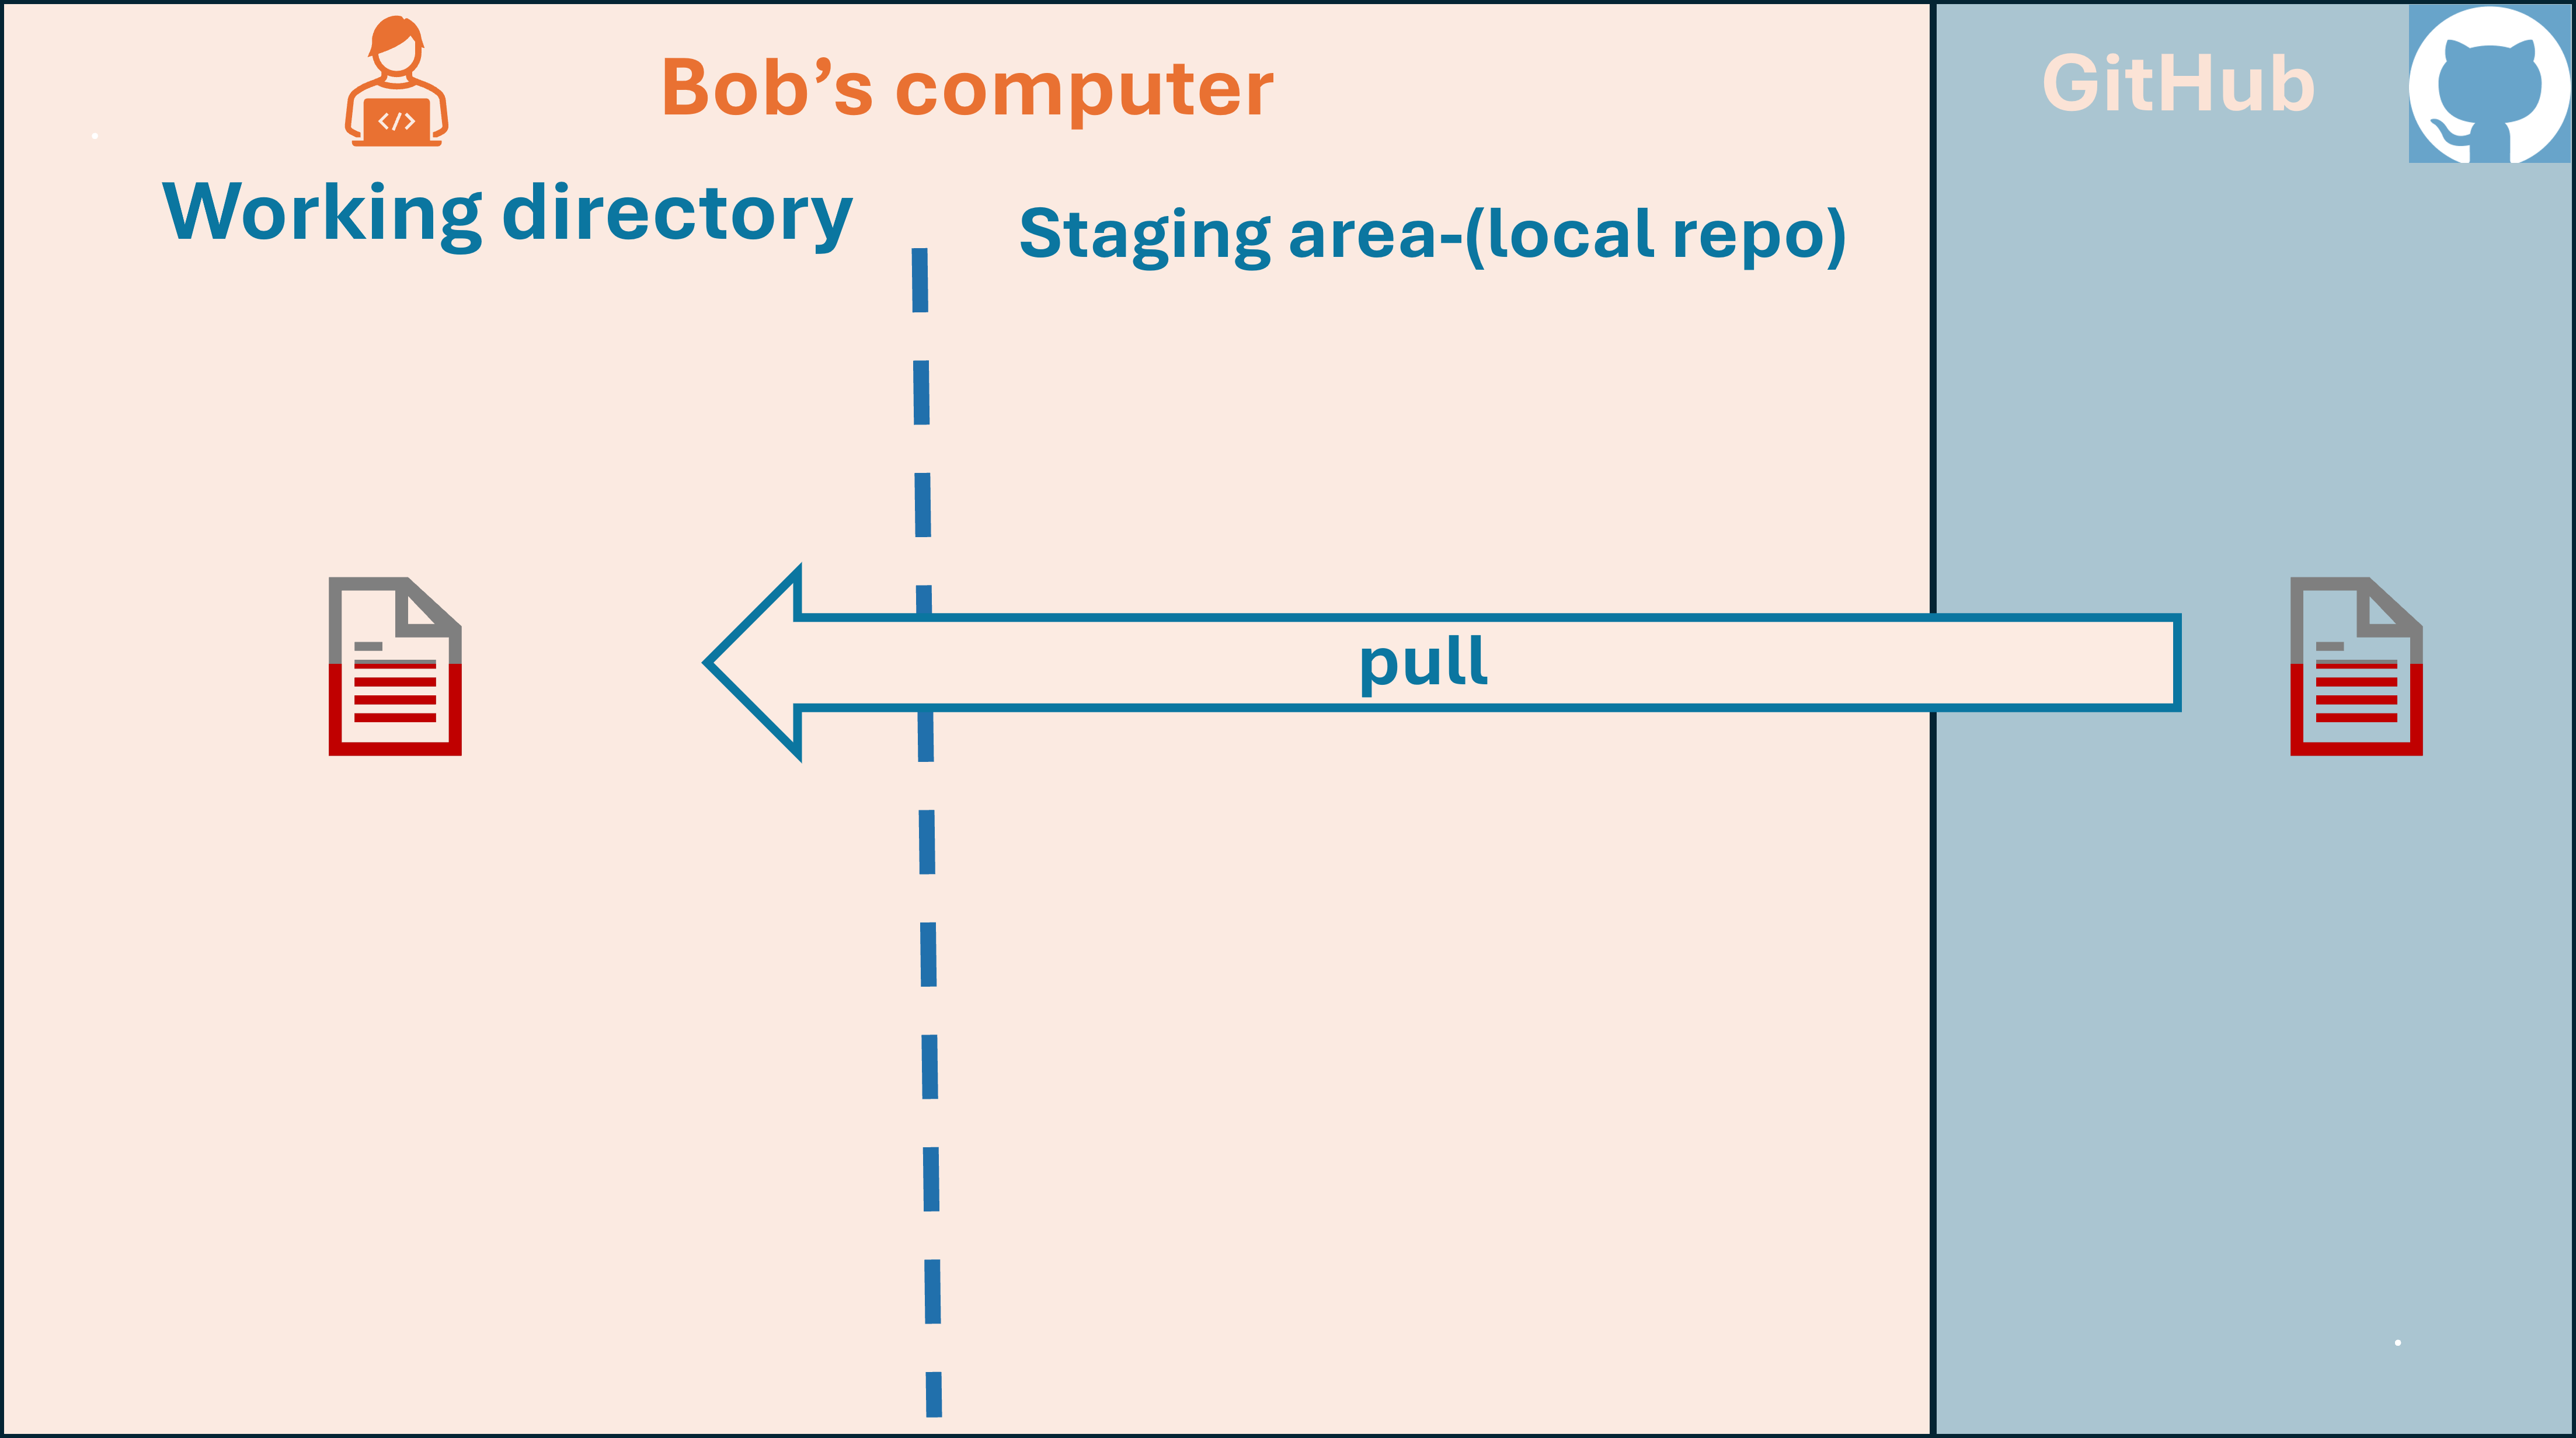
\includegraphics[width=1.0\textwidth]{GitPrinciple8N.png} \\ }
\only<9>{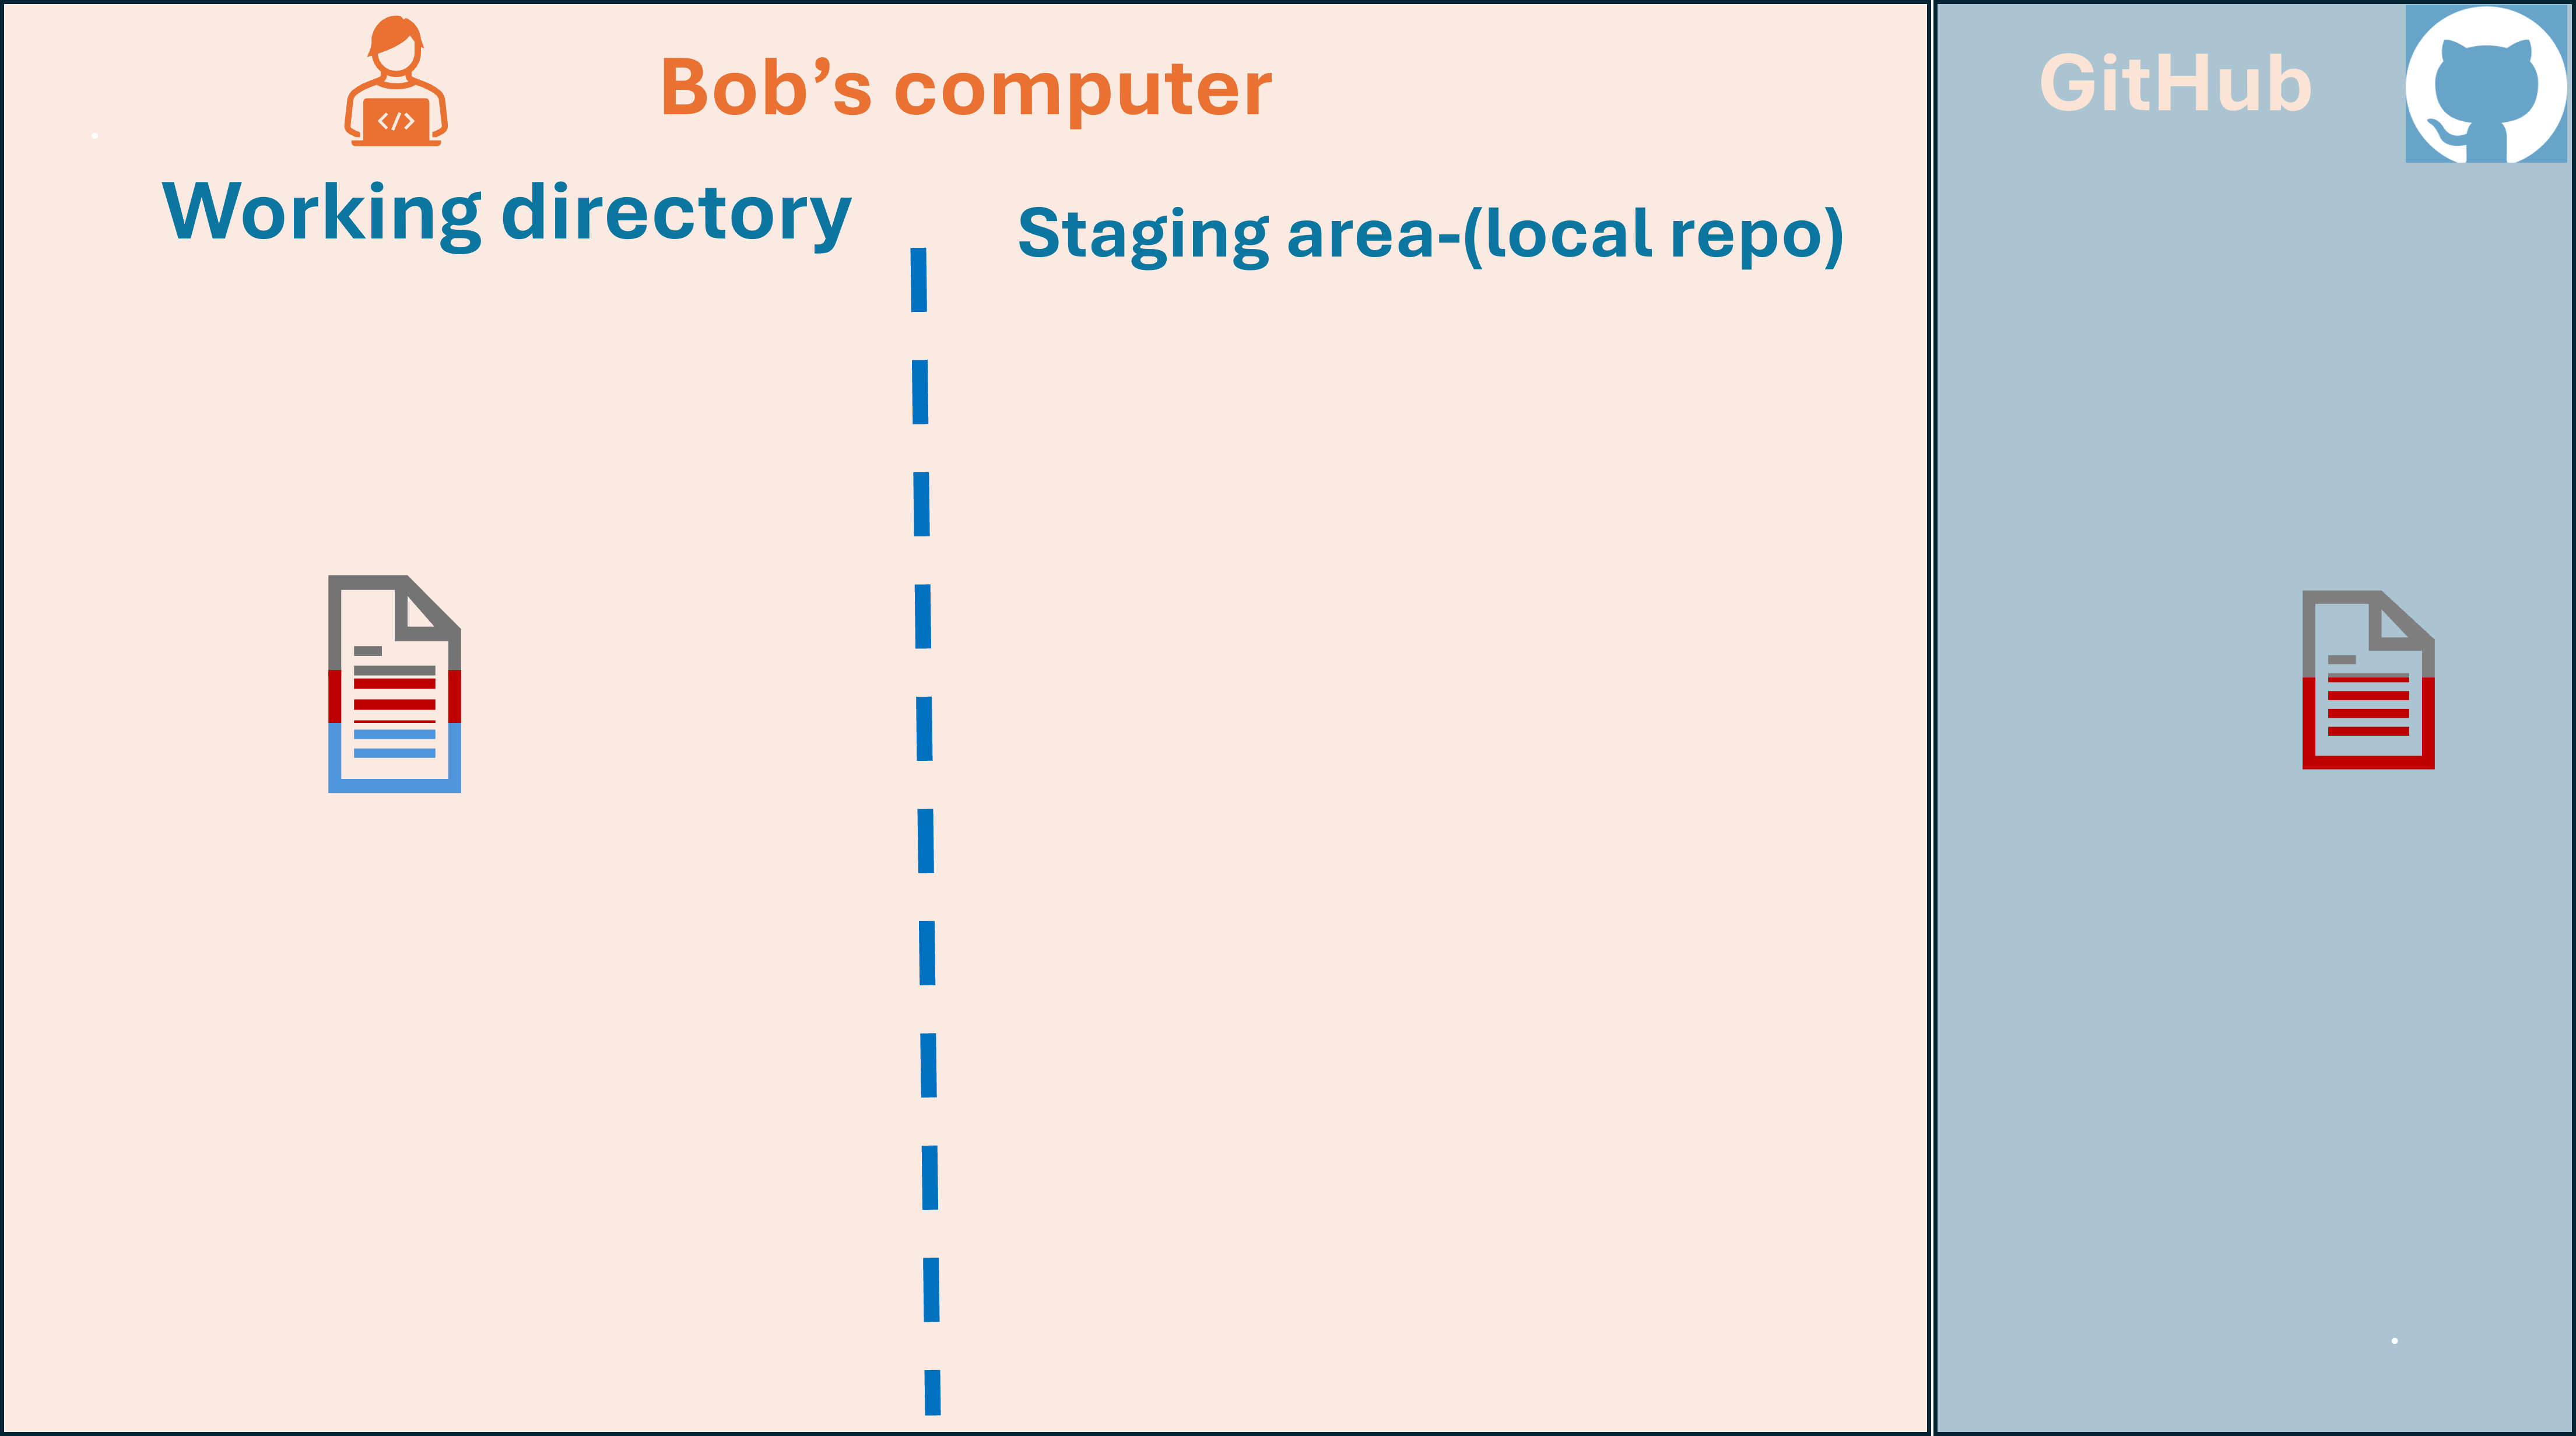
\includegraphics[width=1.0\textwidth]{GitPrinciple9N.png} \\ }
\only<10>{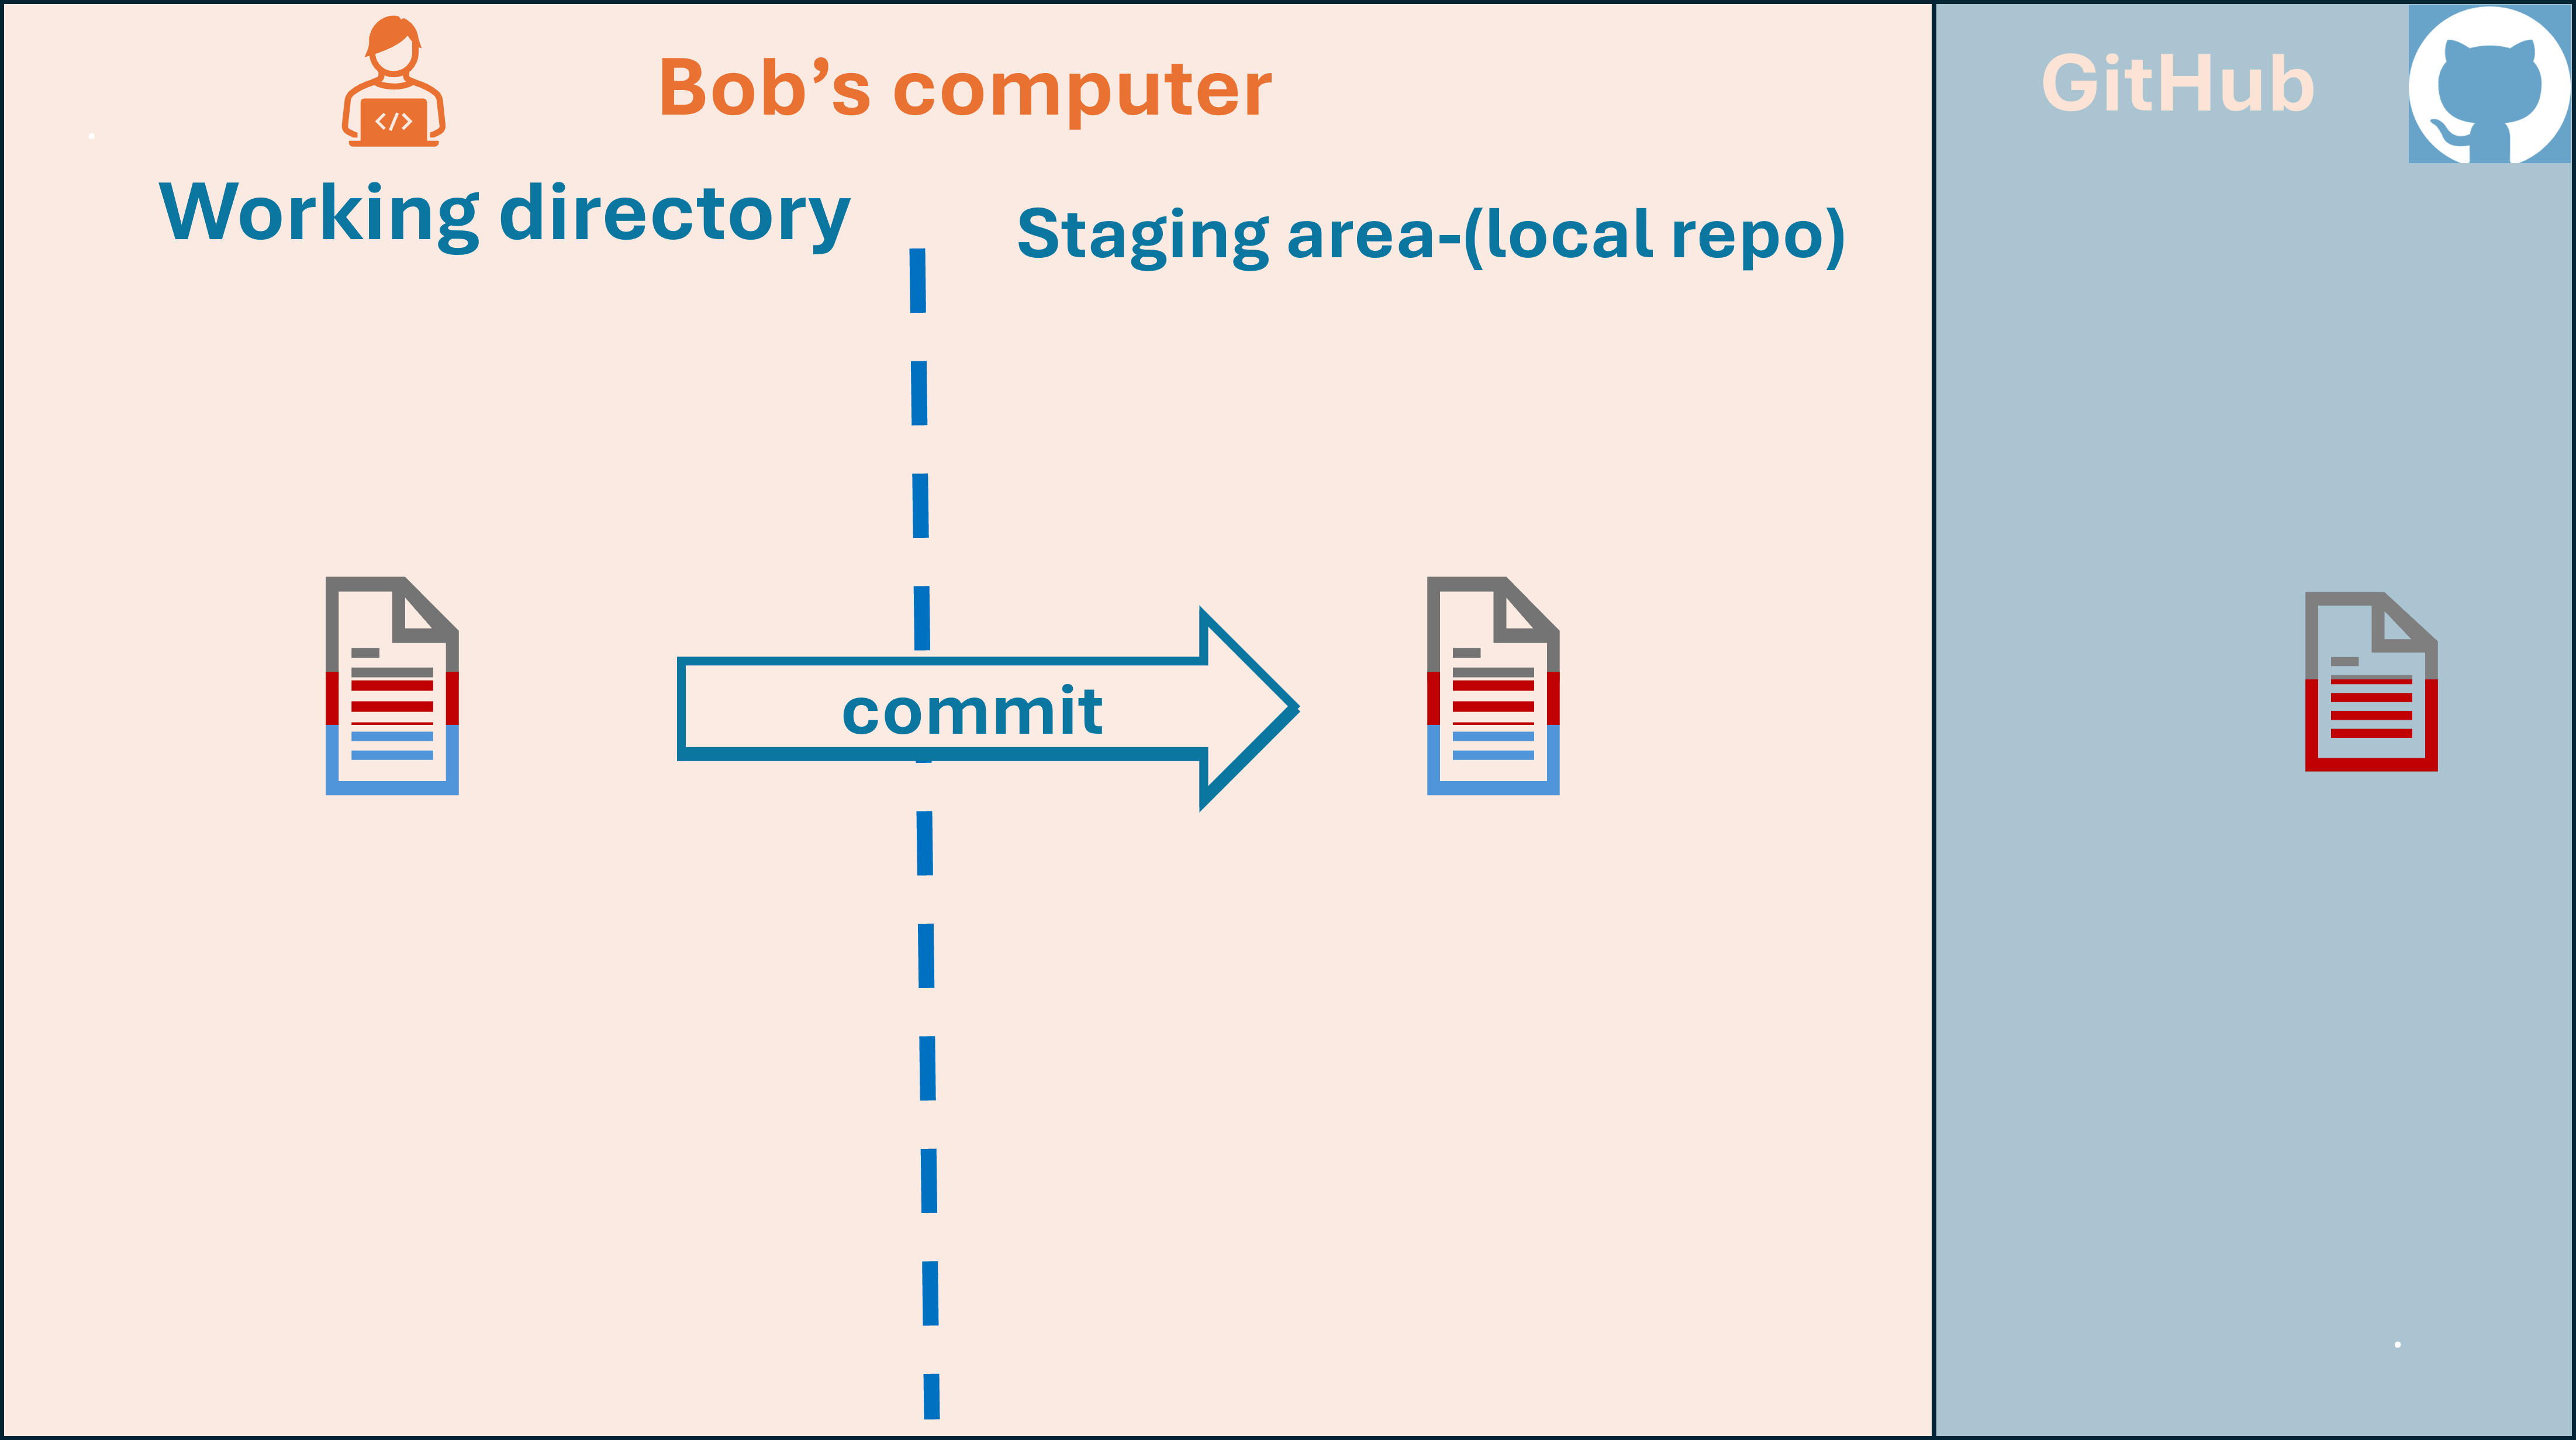
\includegraphics[width=1.0\textwidth]{GitPrinciple10N.png} \\ }
\only<11>{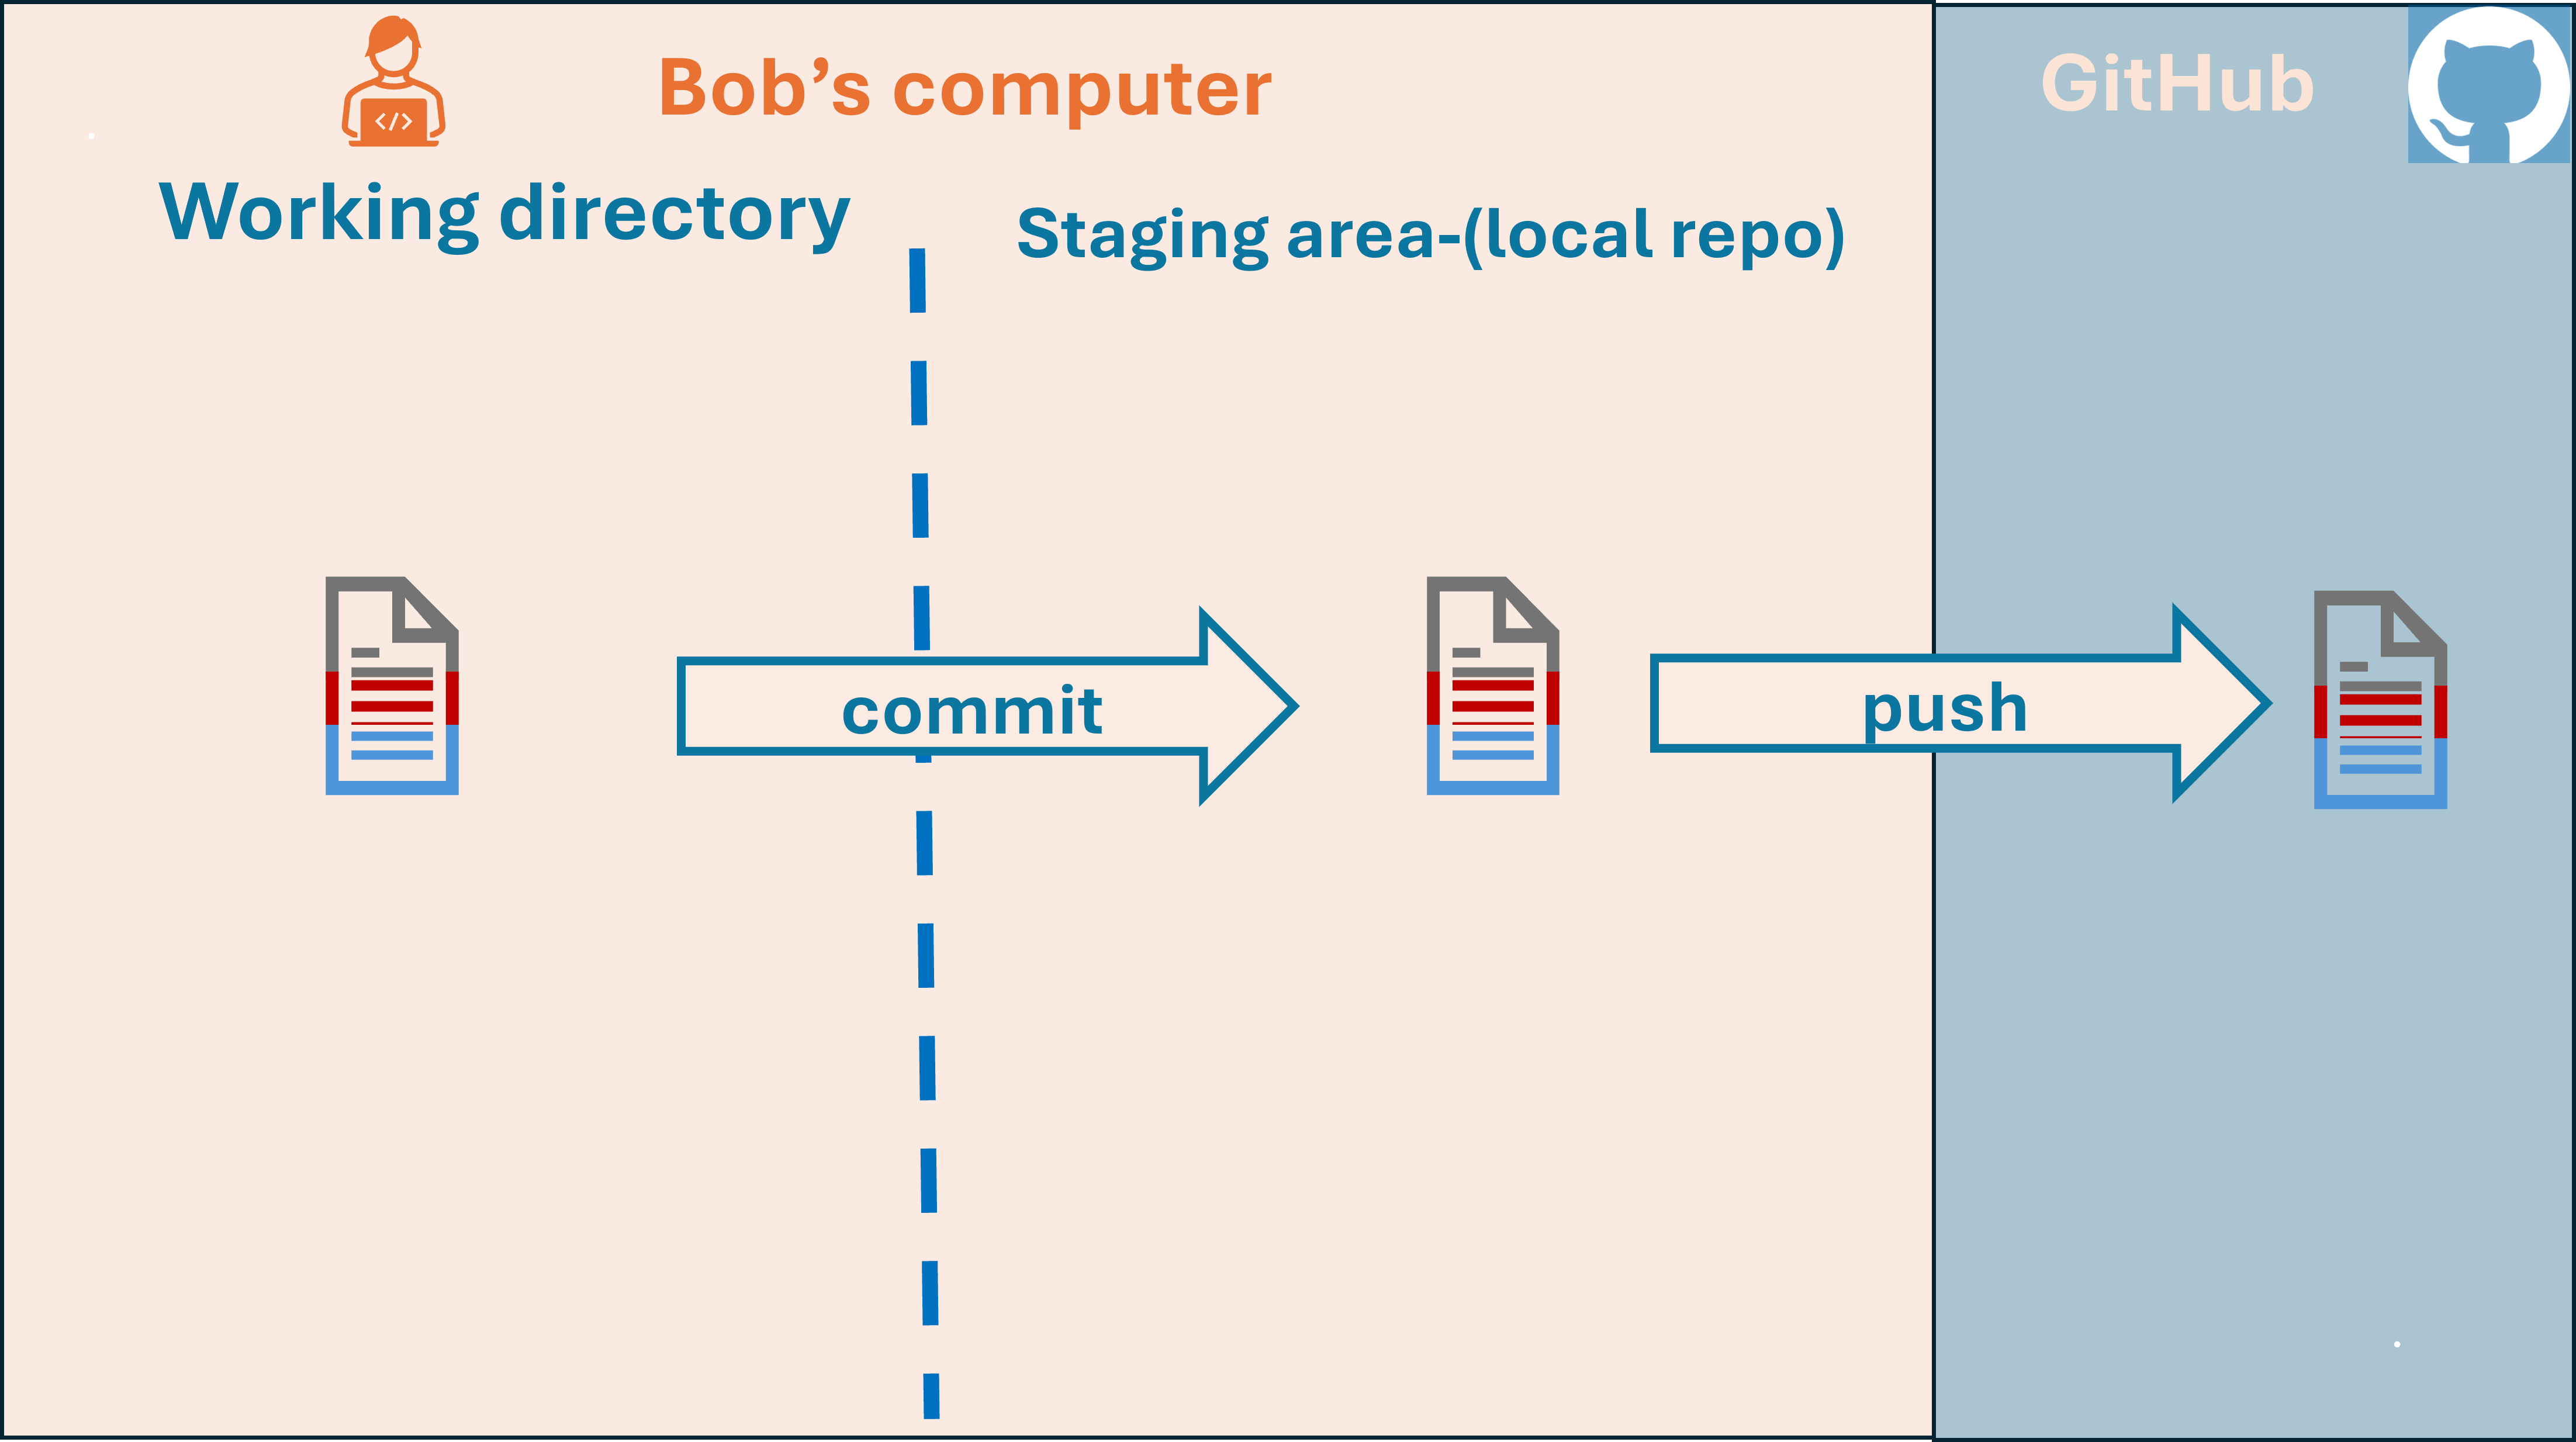
\includegraphics[width=1.0\textwidth]{GitPrinciple11N.png} \\ }
\only<12>{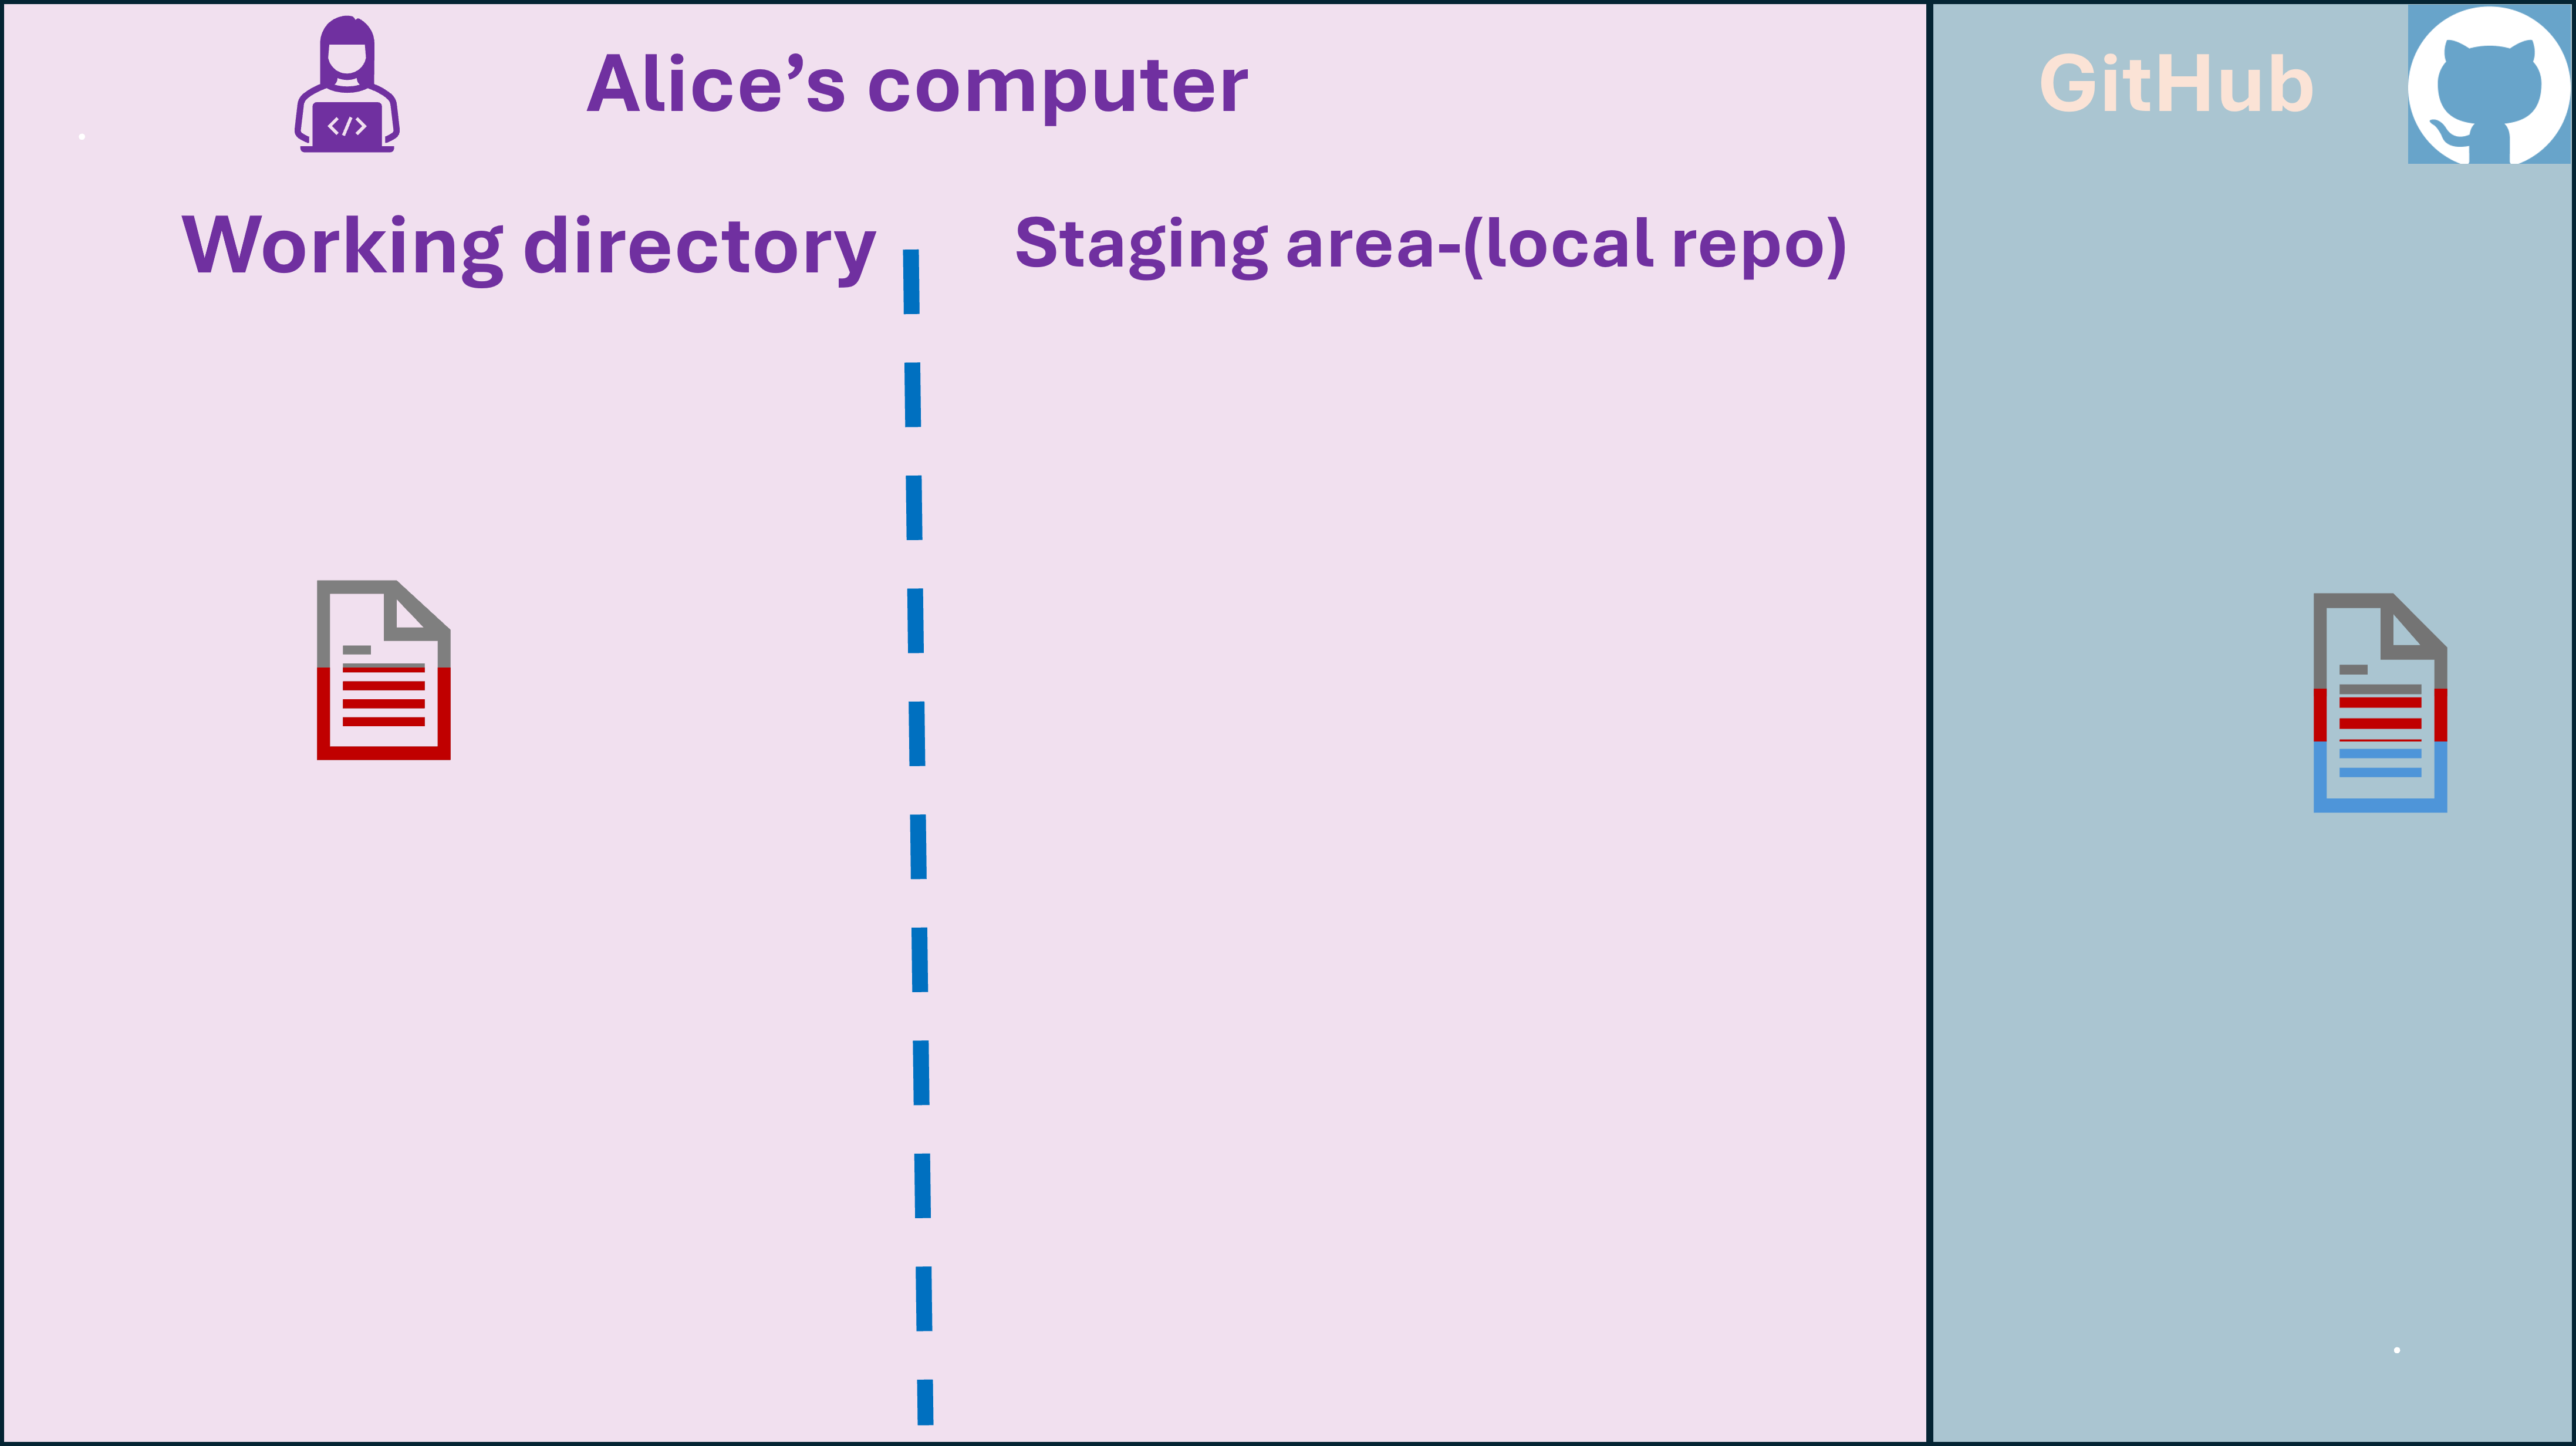
\includegraphics[width=1.0\textwidth]{GitPrinciple12N.png} \\ }
\only<13>{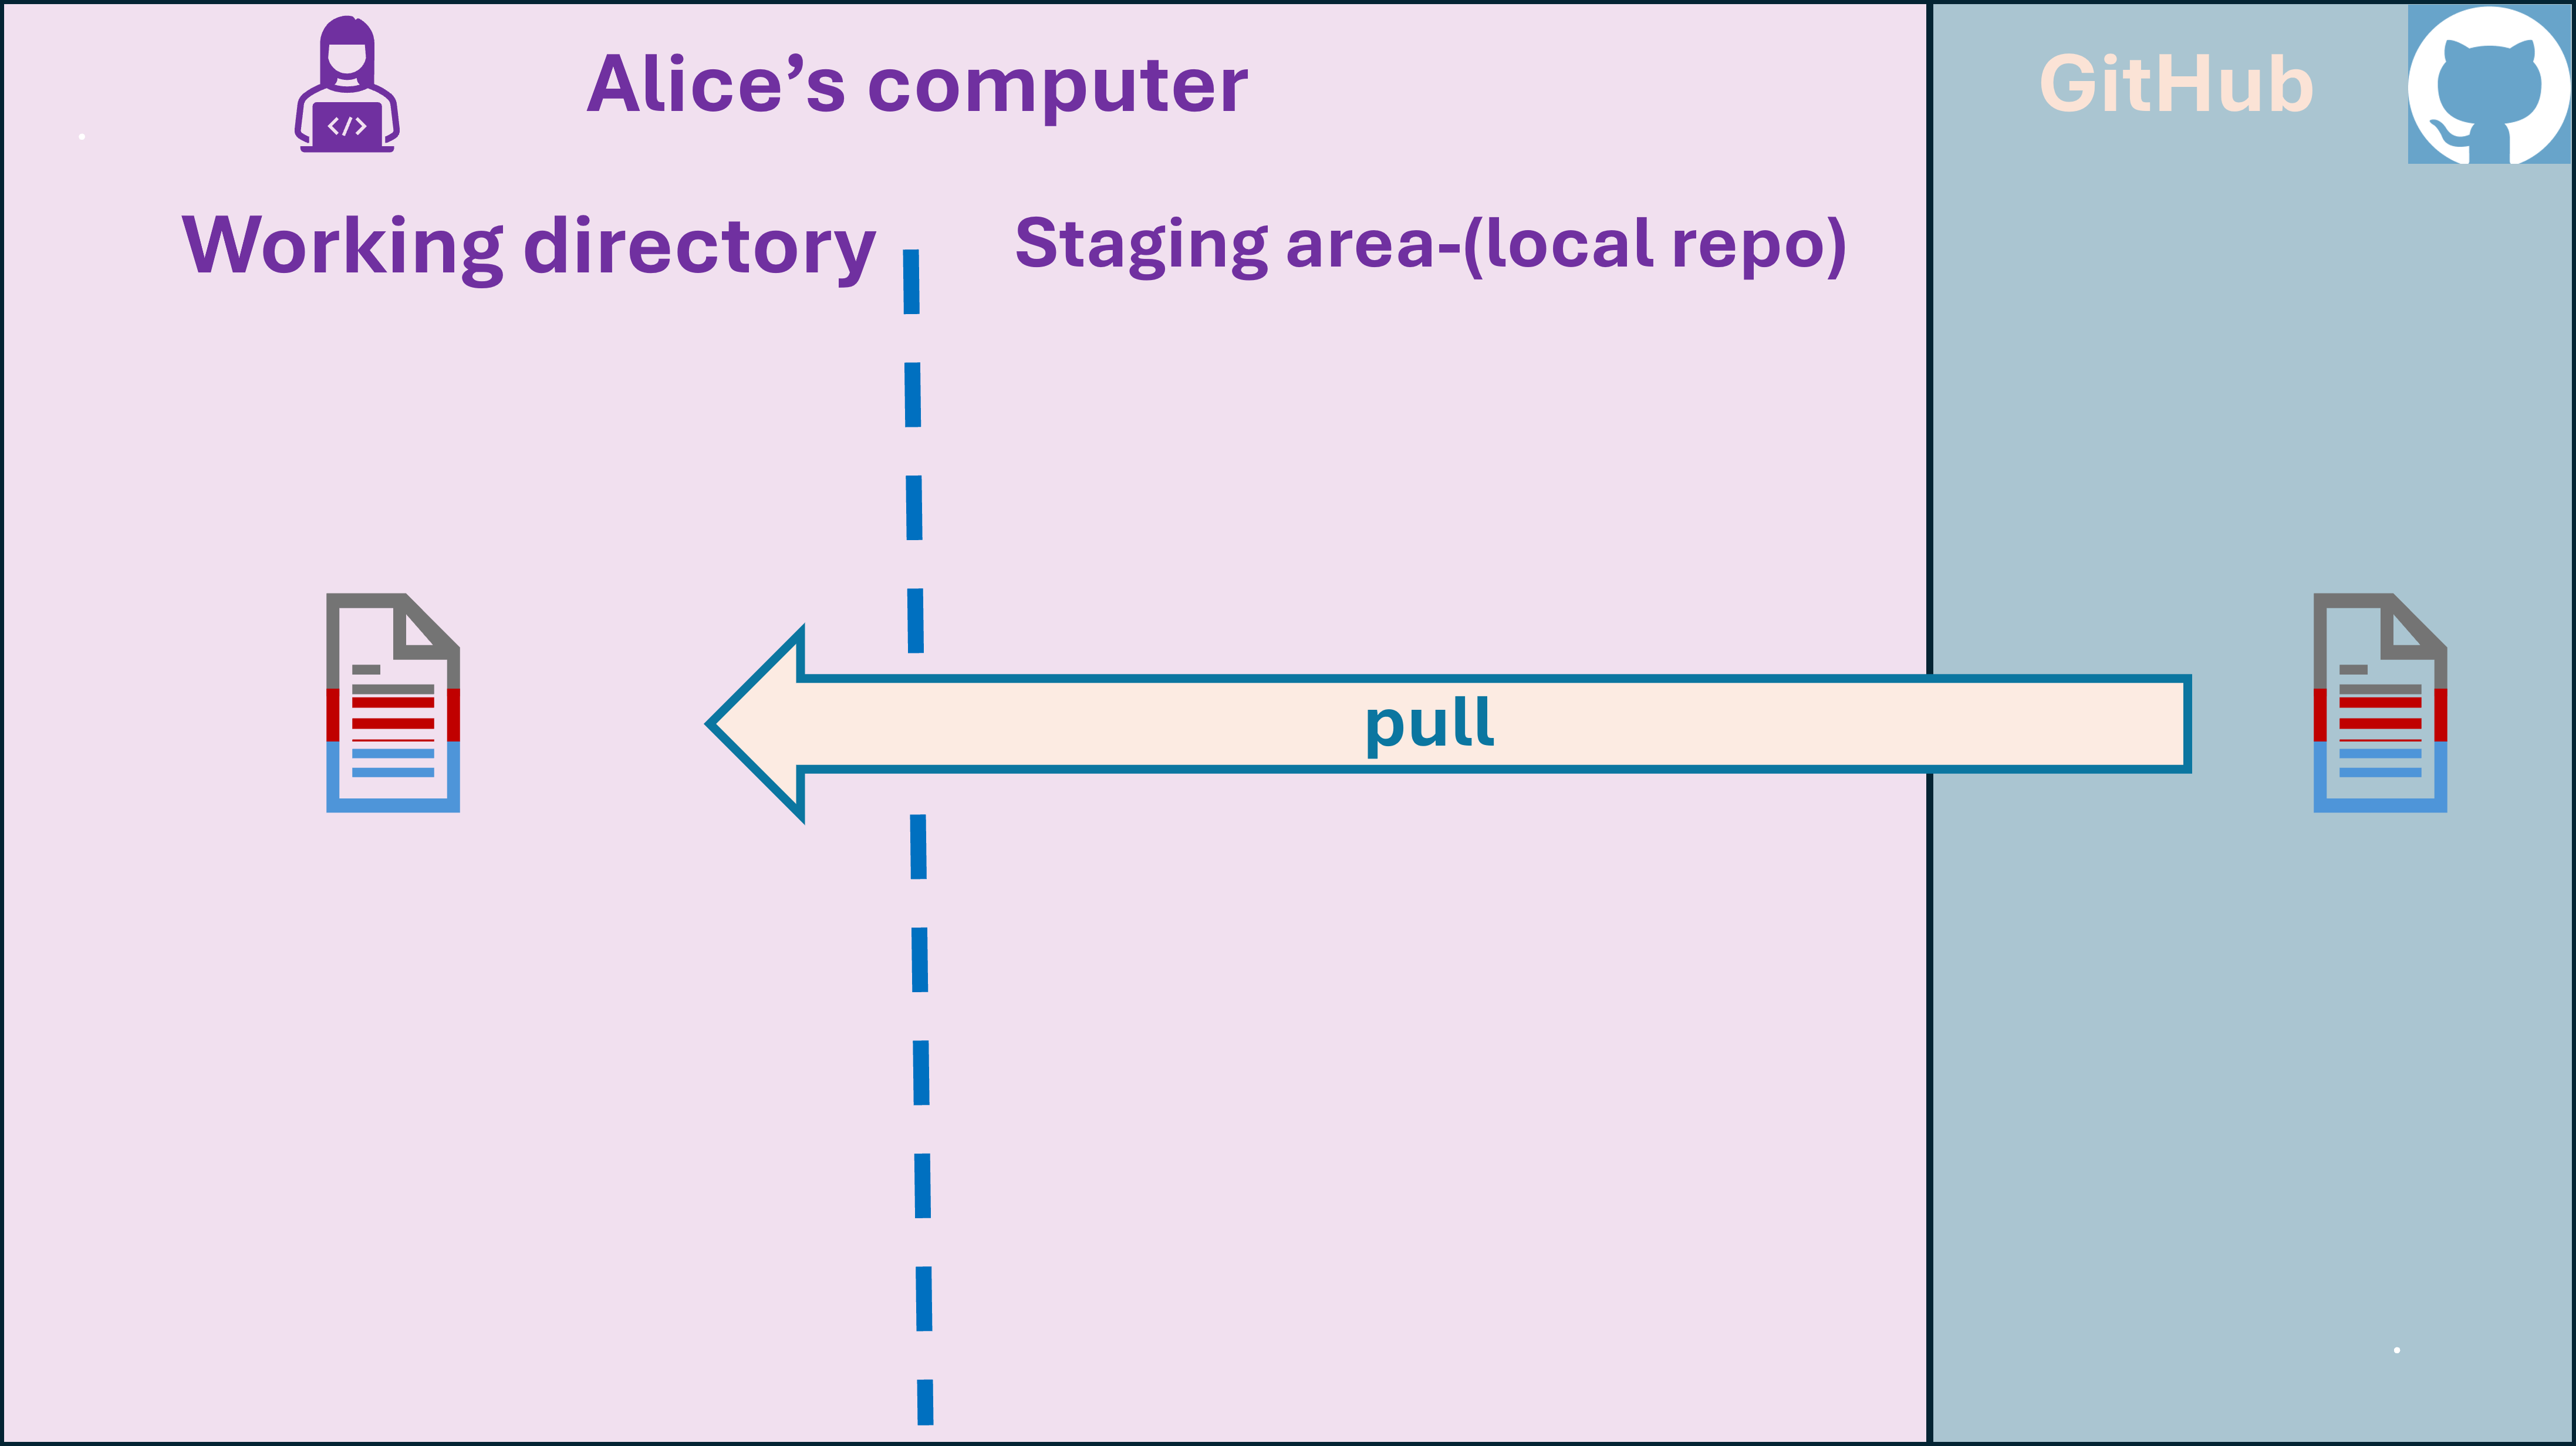
\includegraphics[width=1.0\textwidth]{GitPrinciple13N.png} \\ }
\end{itemize}
\end{frame}

\subsection{Issues}

\begin{frame}
\frametitle{Remarks and issues}
    \begin{itemize}[<+->]
     \item A commit can include changes from multiple files simultaneously
     \item One can do several commits before pushing (to GitHub)
     \item Commit messages can be edited (\texttt{amend})
     \item Every commit has an identifier (\texttt{hash} or \texttt{SHA})
     \item Git manage complex situations
     \item Many actions available directly in Visual Studio
    \end{itemize}
\end{frame}

\begin{frame}
\frametitle{Git for collaborating: Complex situations}
\textcolor{violet}{\textbf{Alice}} and \textcolor{orange}{\textbf{Bob}} work on the same file \textbf{at the same time}
\pause
\begin{itemize}
\item[]
\only<1>{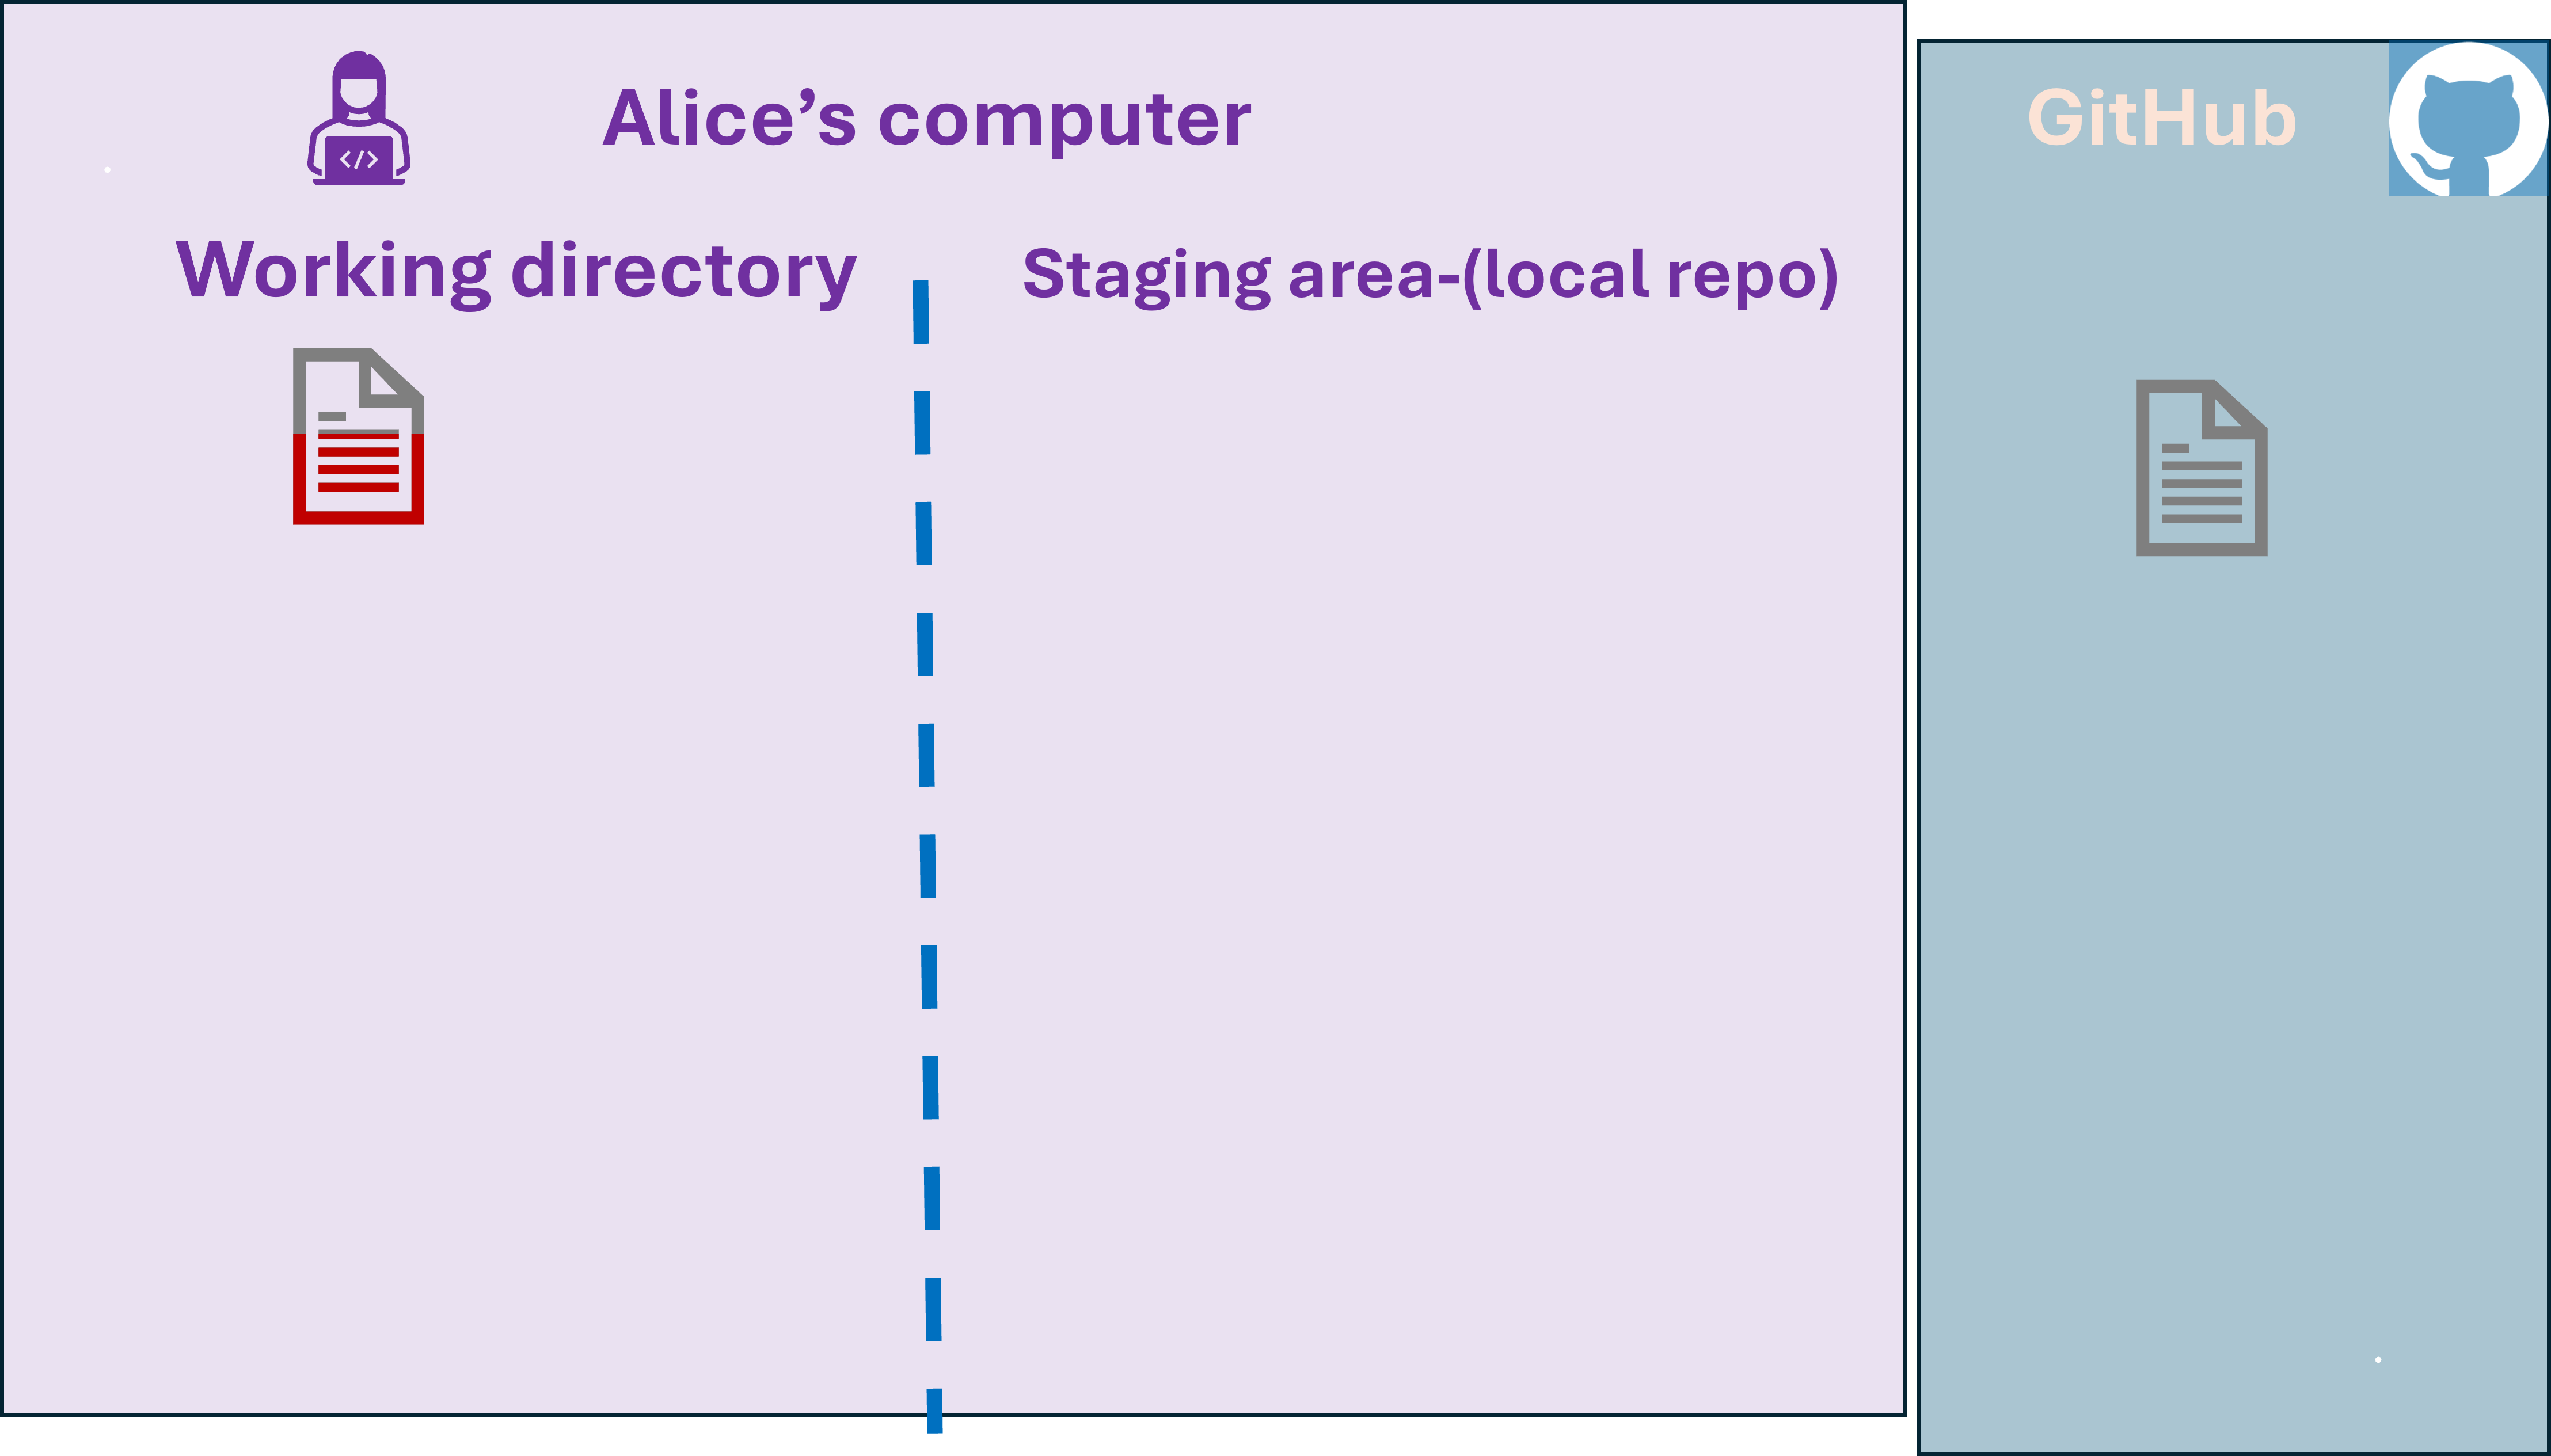
\includegraphics[width=1.0\textwidth]{GitComplex2N.png} \\ }
\only<2>{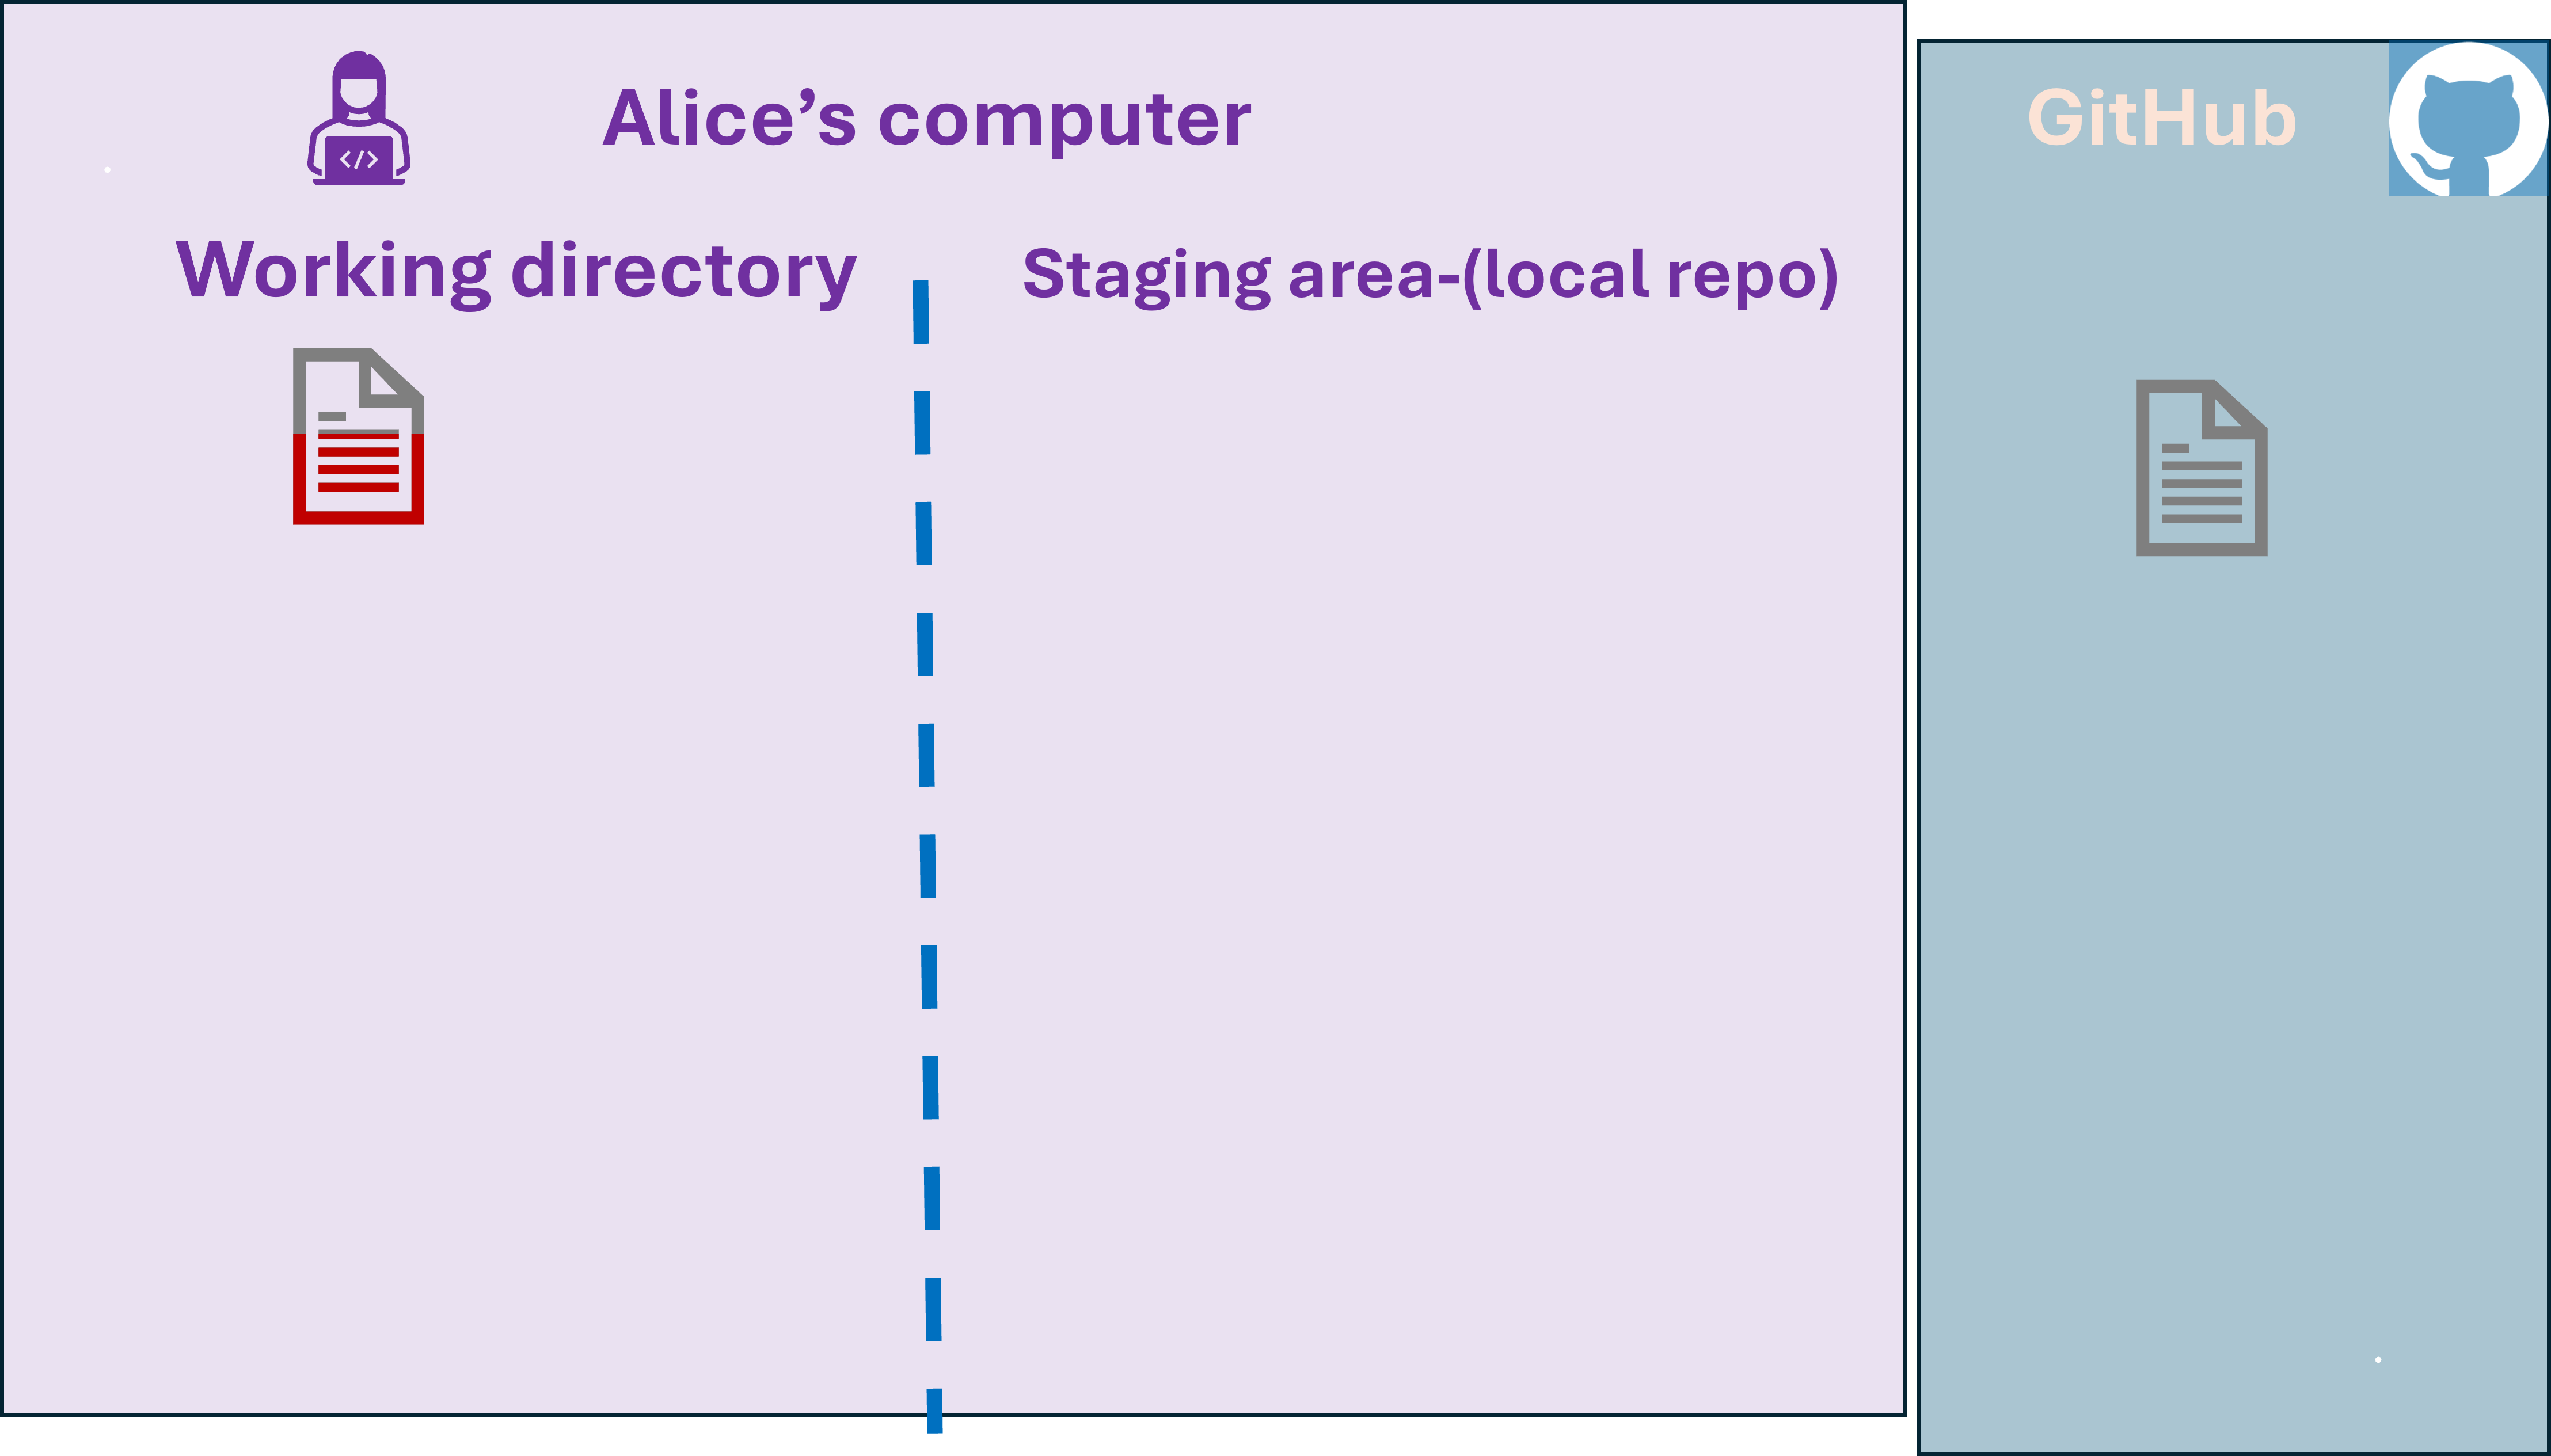
\includegraphics[width=1.0\textwidth]{GitComplex2N.png} \\ }
\only<3>{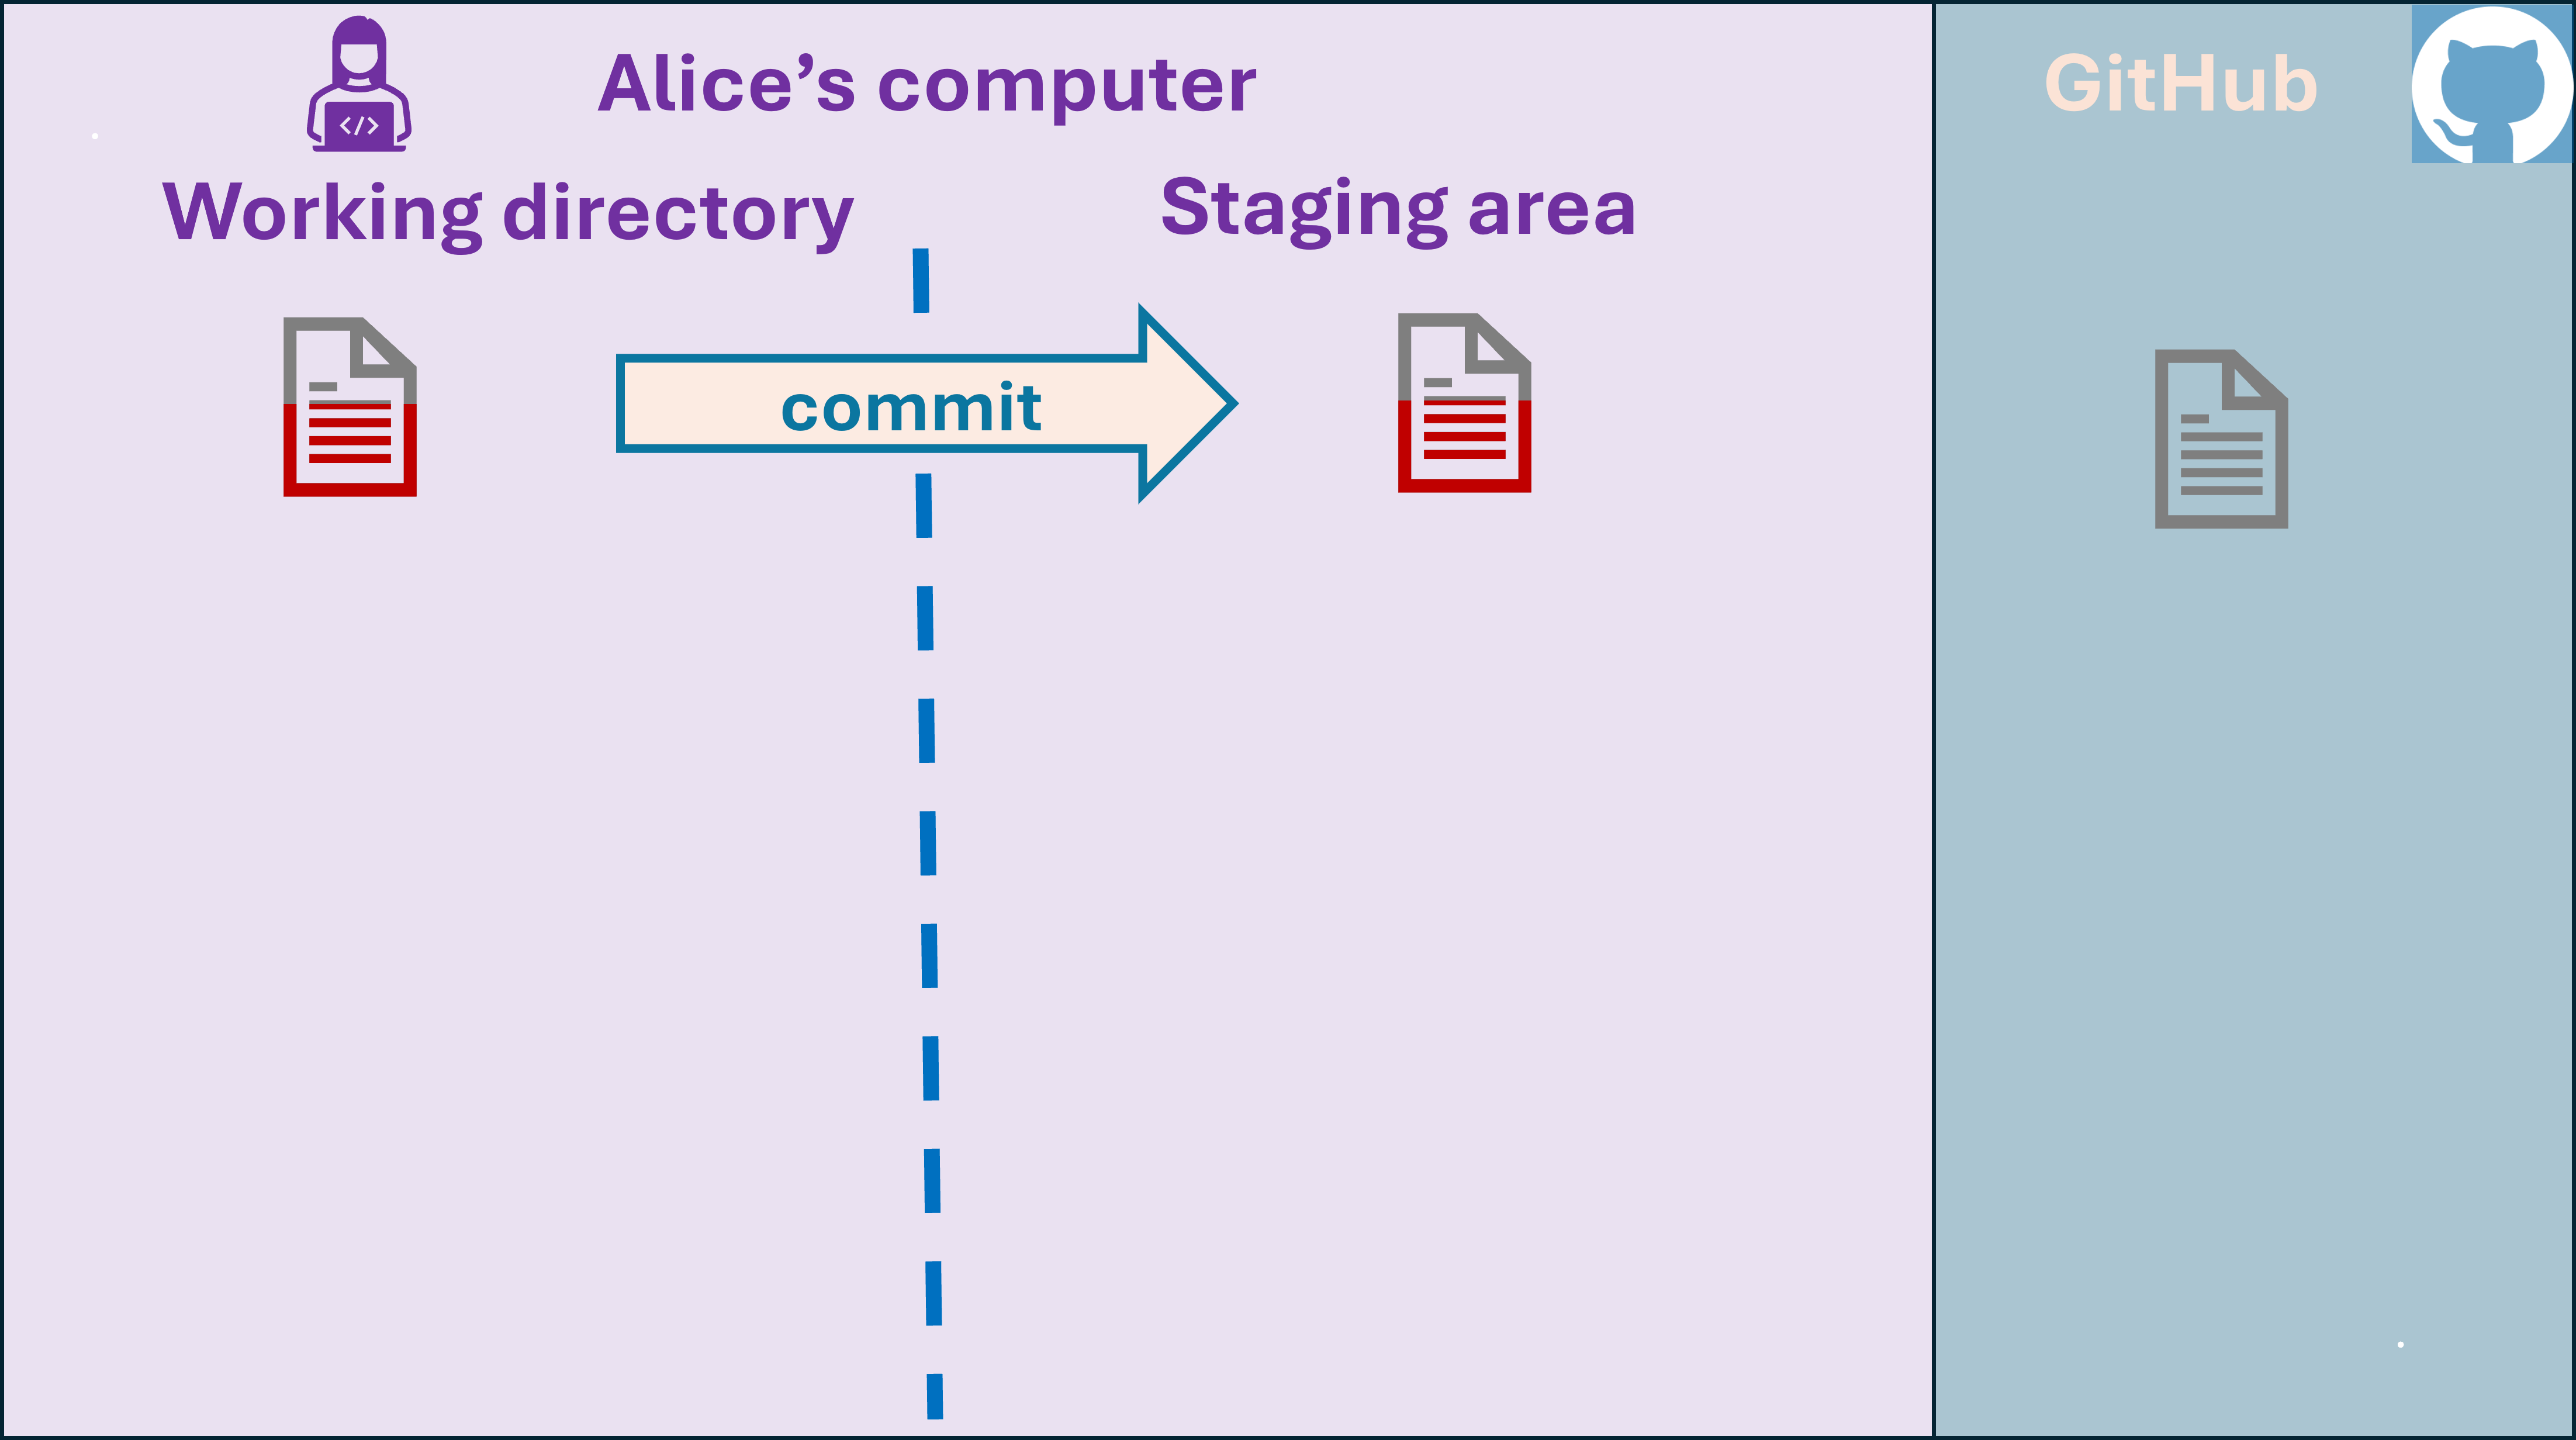
\includegraphics[width=1.0\textwidth]{GitComplex3N.png} \\ }
\only<4>{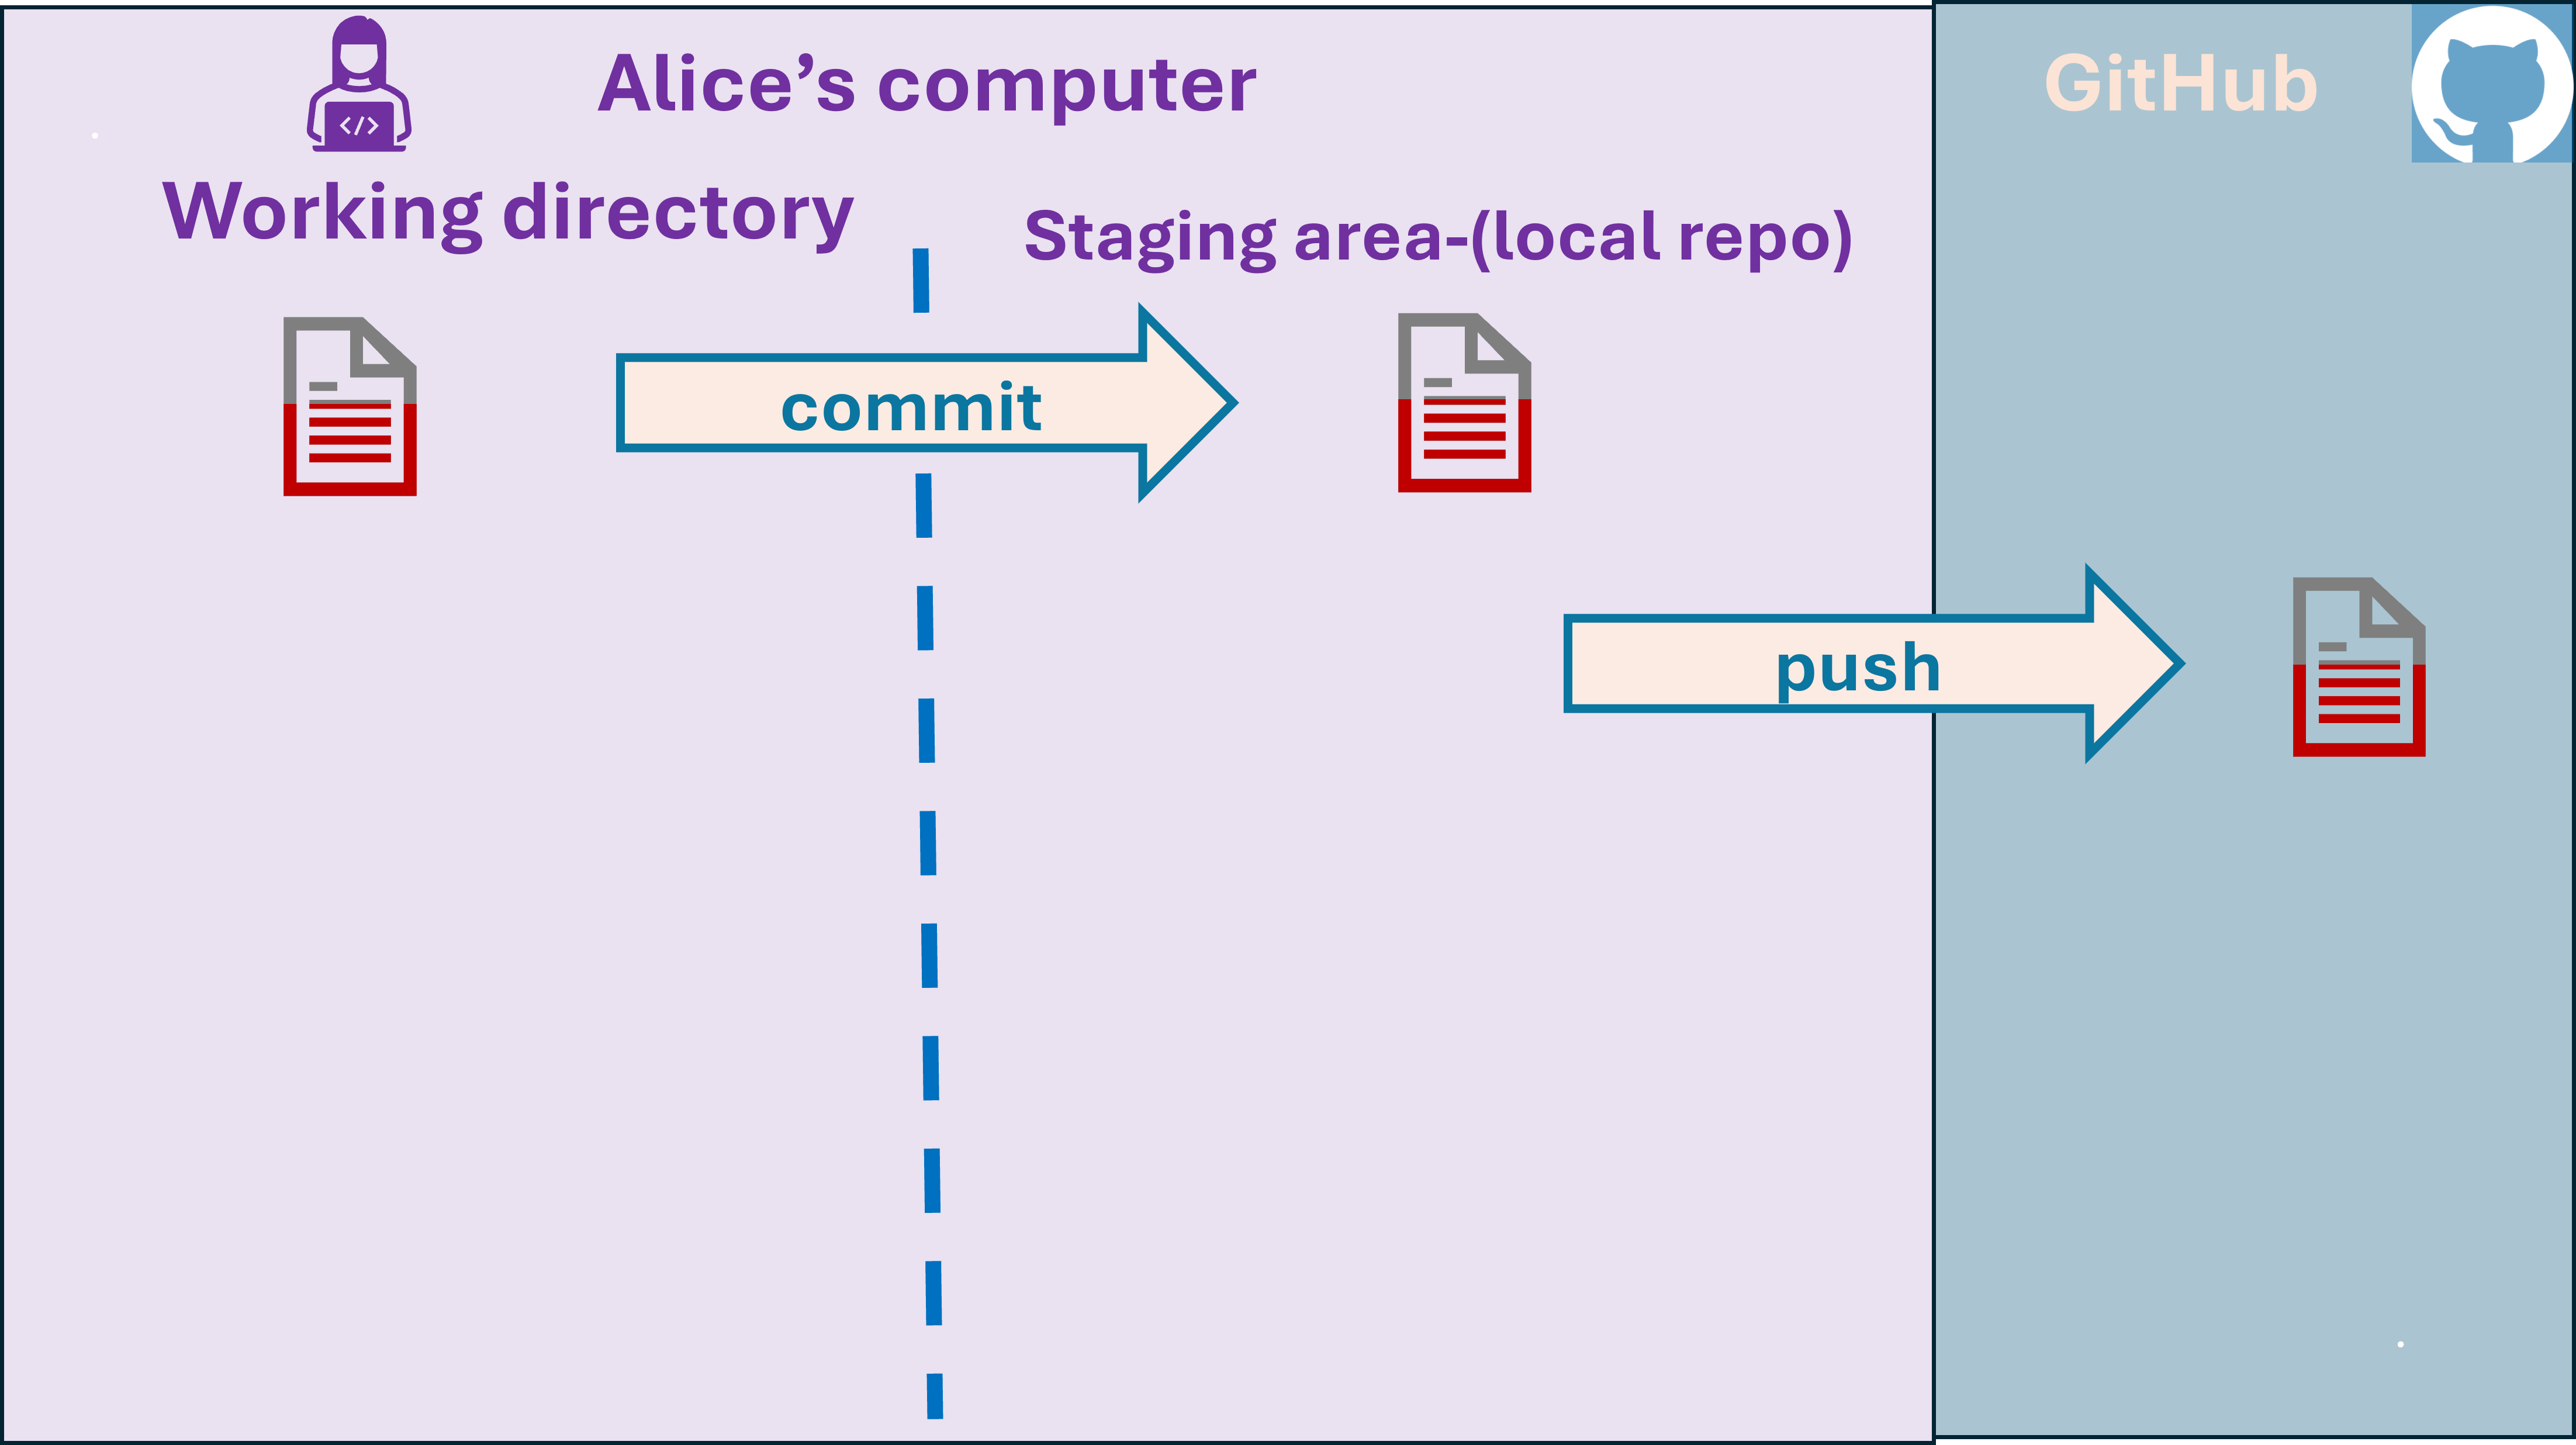
\includegraphics[width=1.0\textwidth]{GitComplex4N.png} \\ }
\only<5>{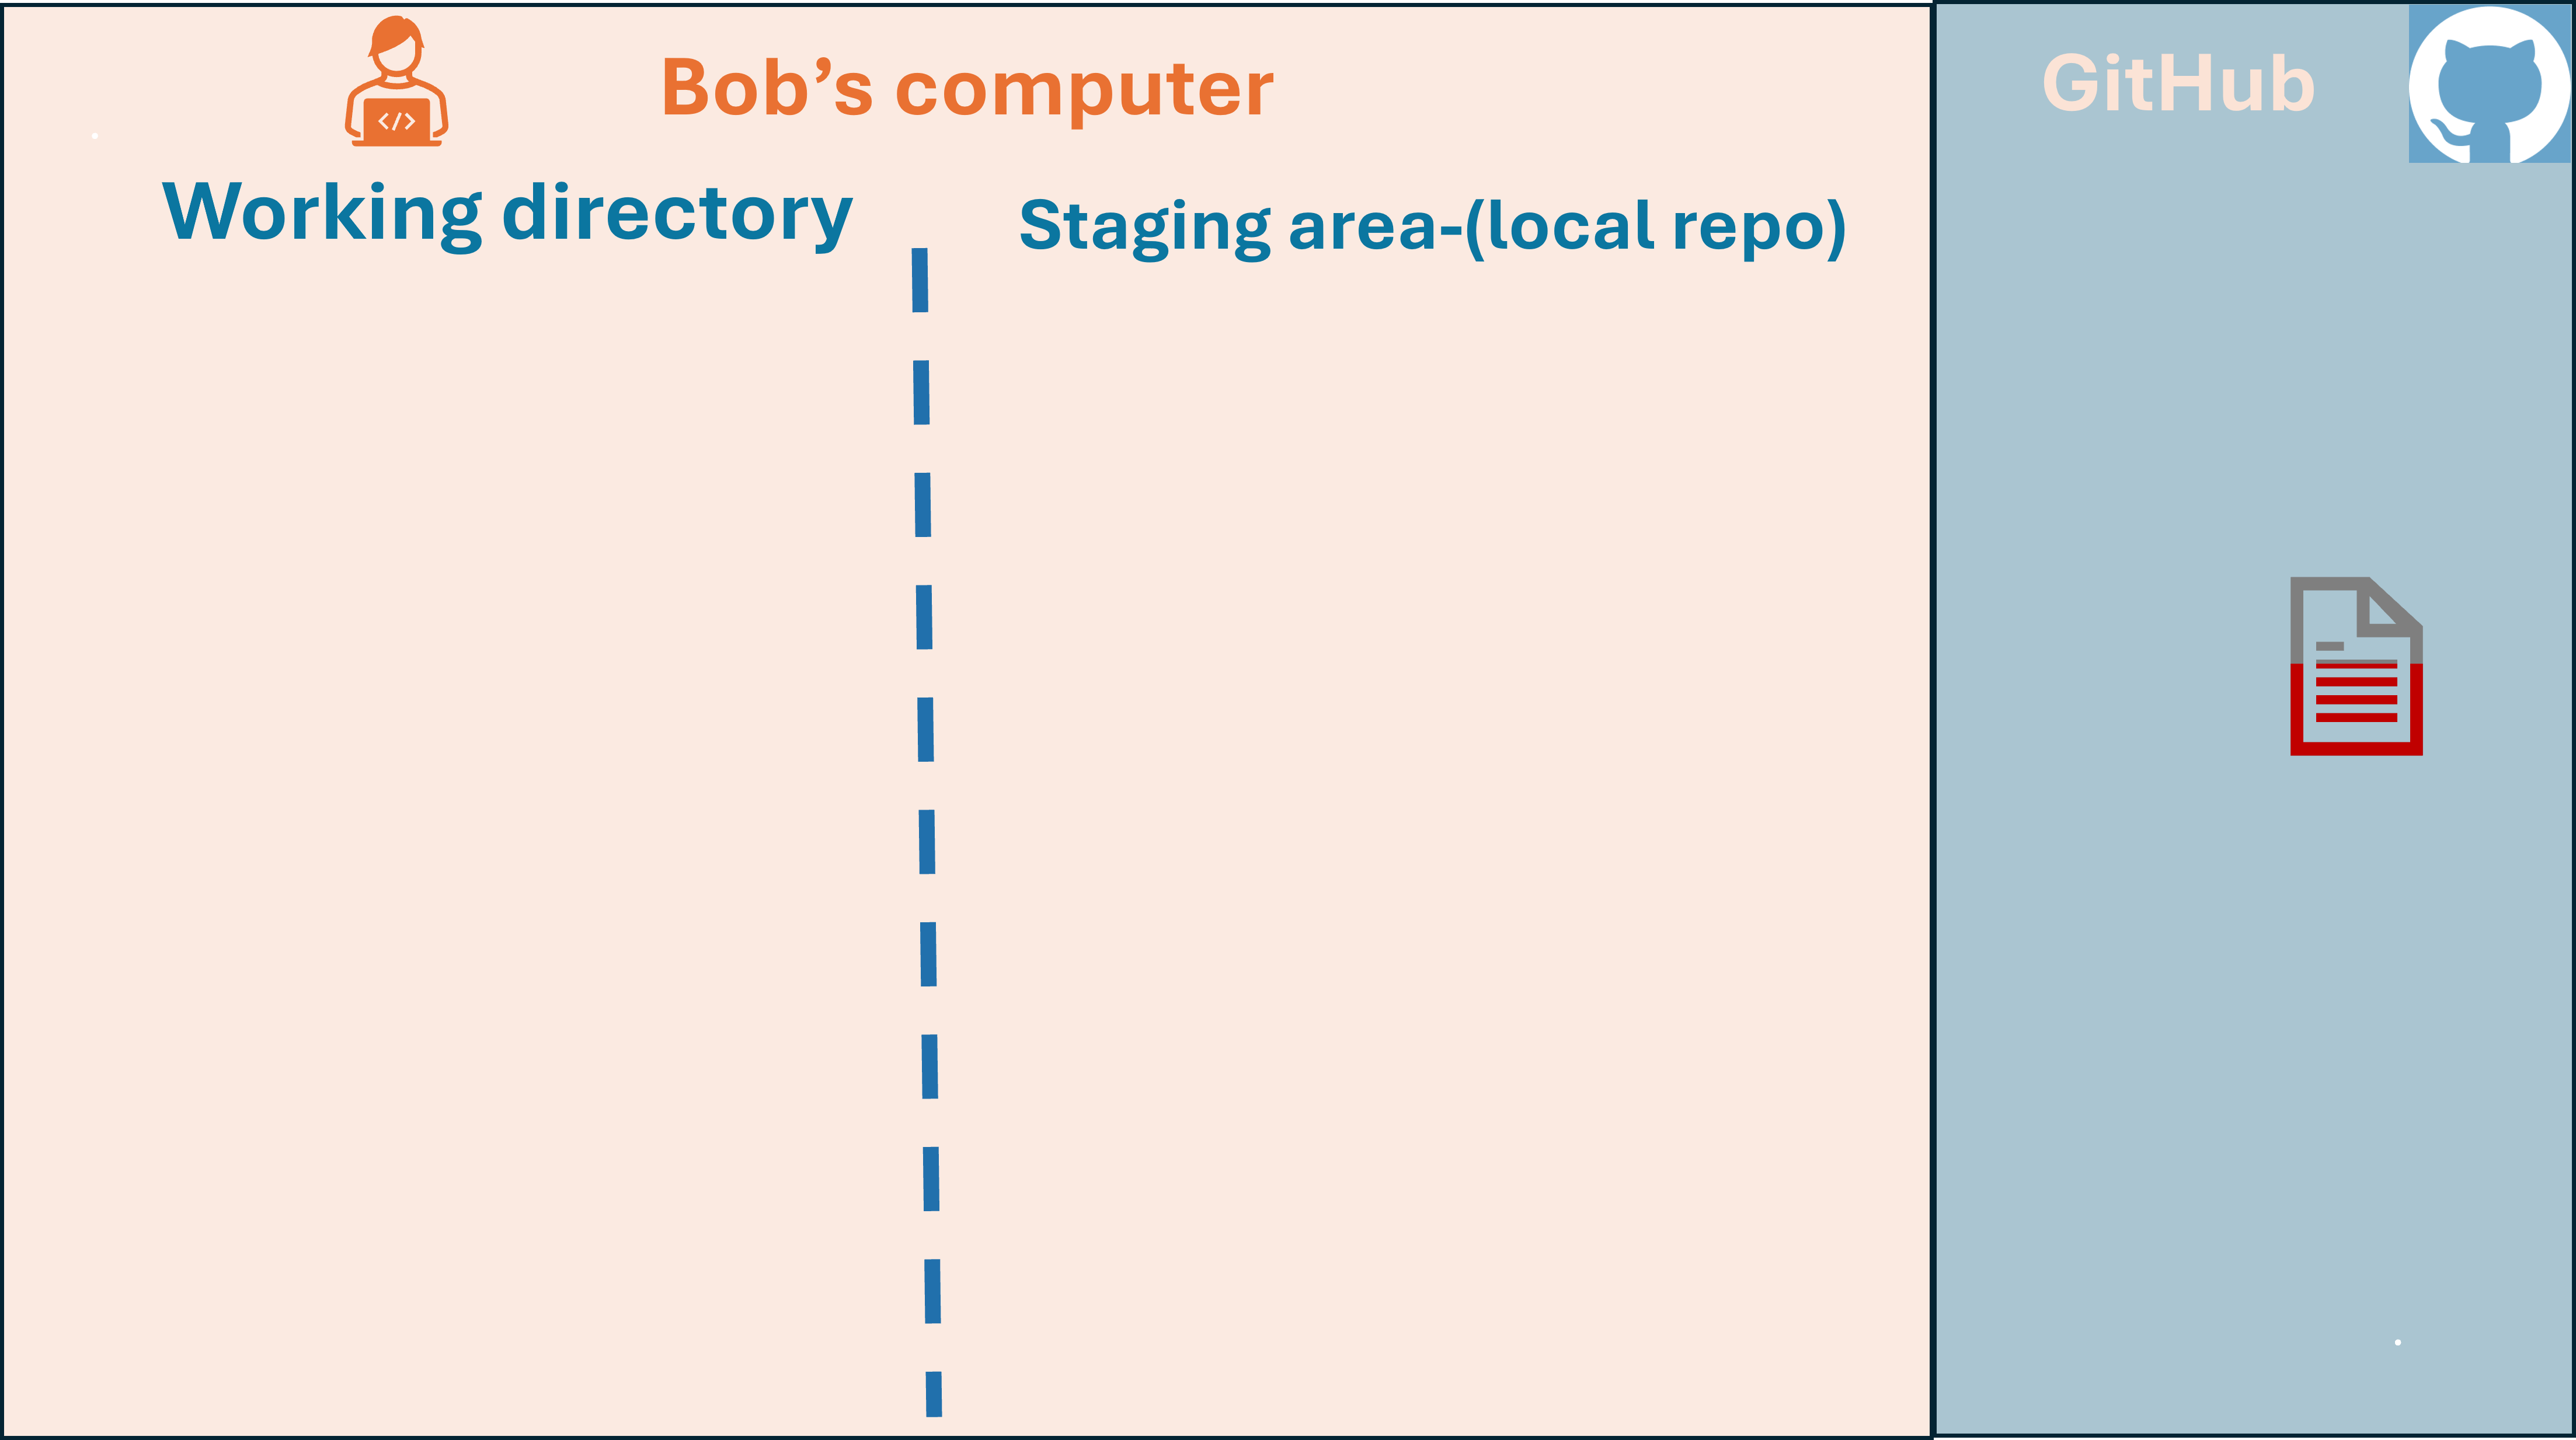
\includegraphics[width=1.0\textwidth]{GitComplex5N.png} \\ }
\only<6>{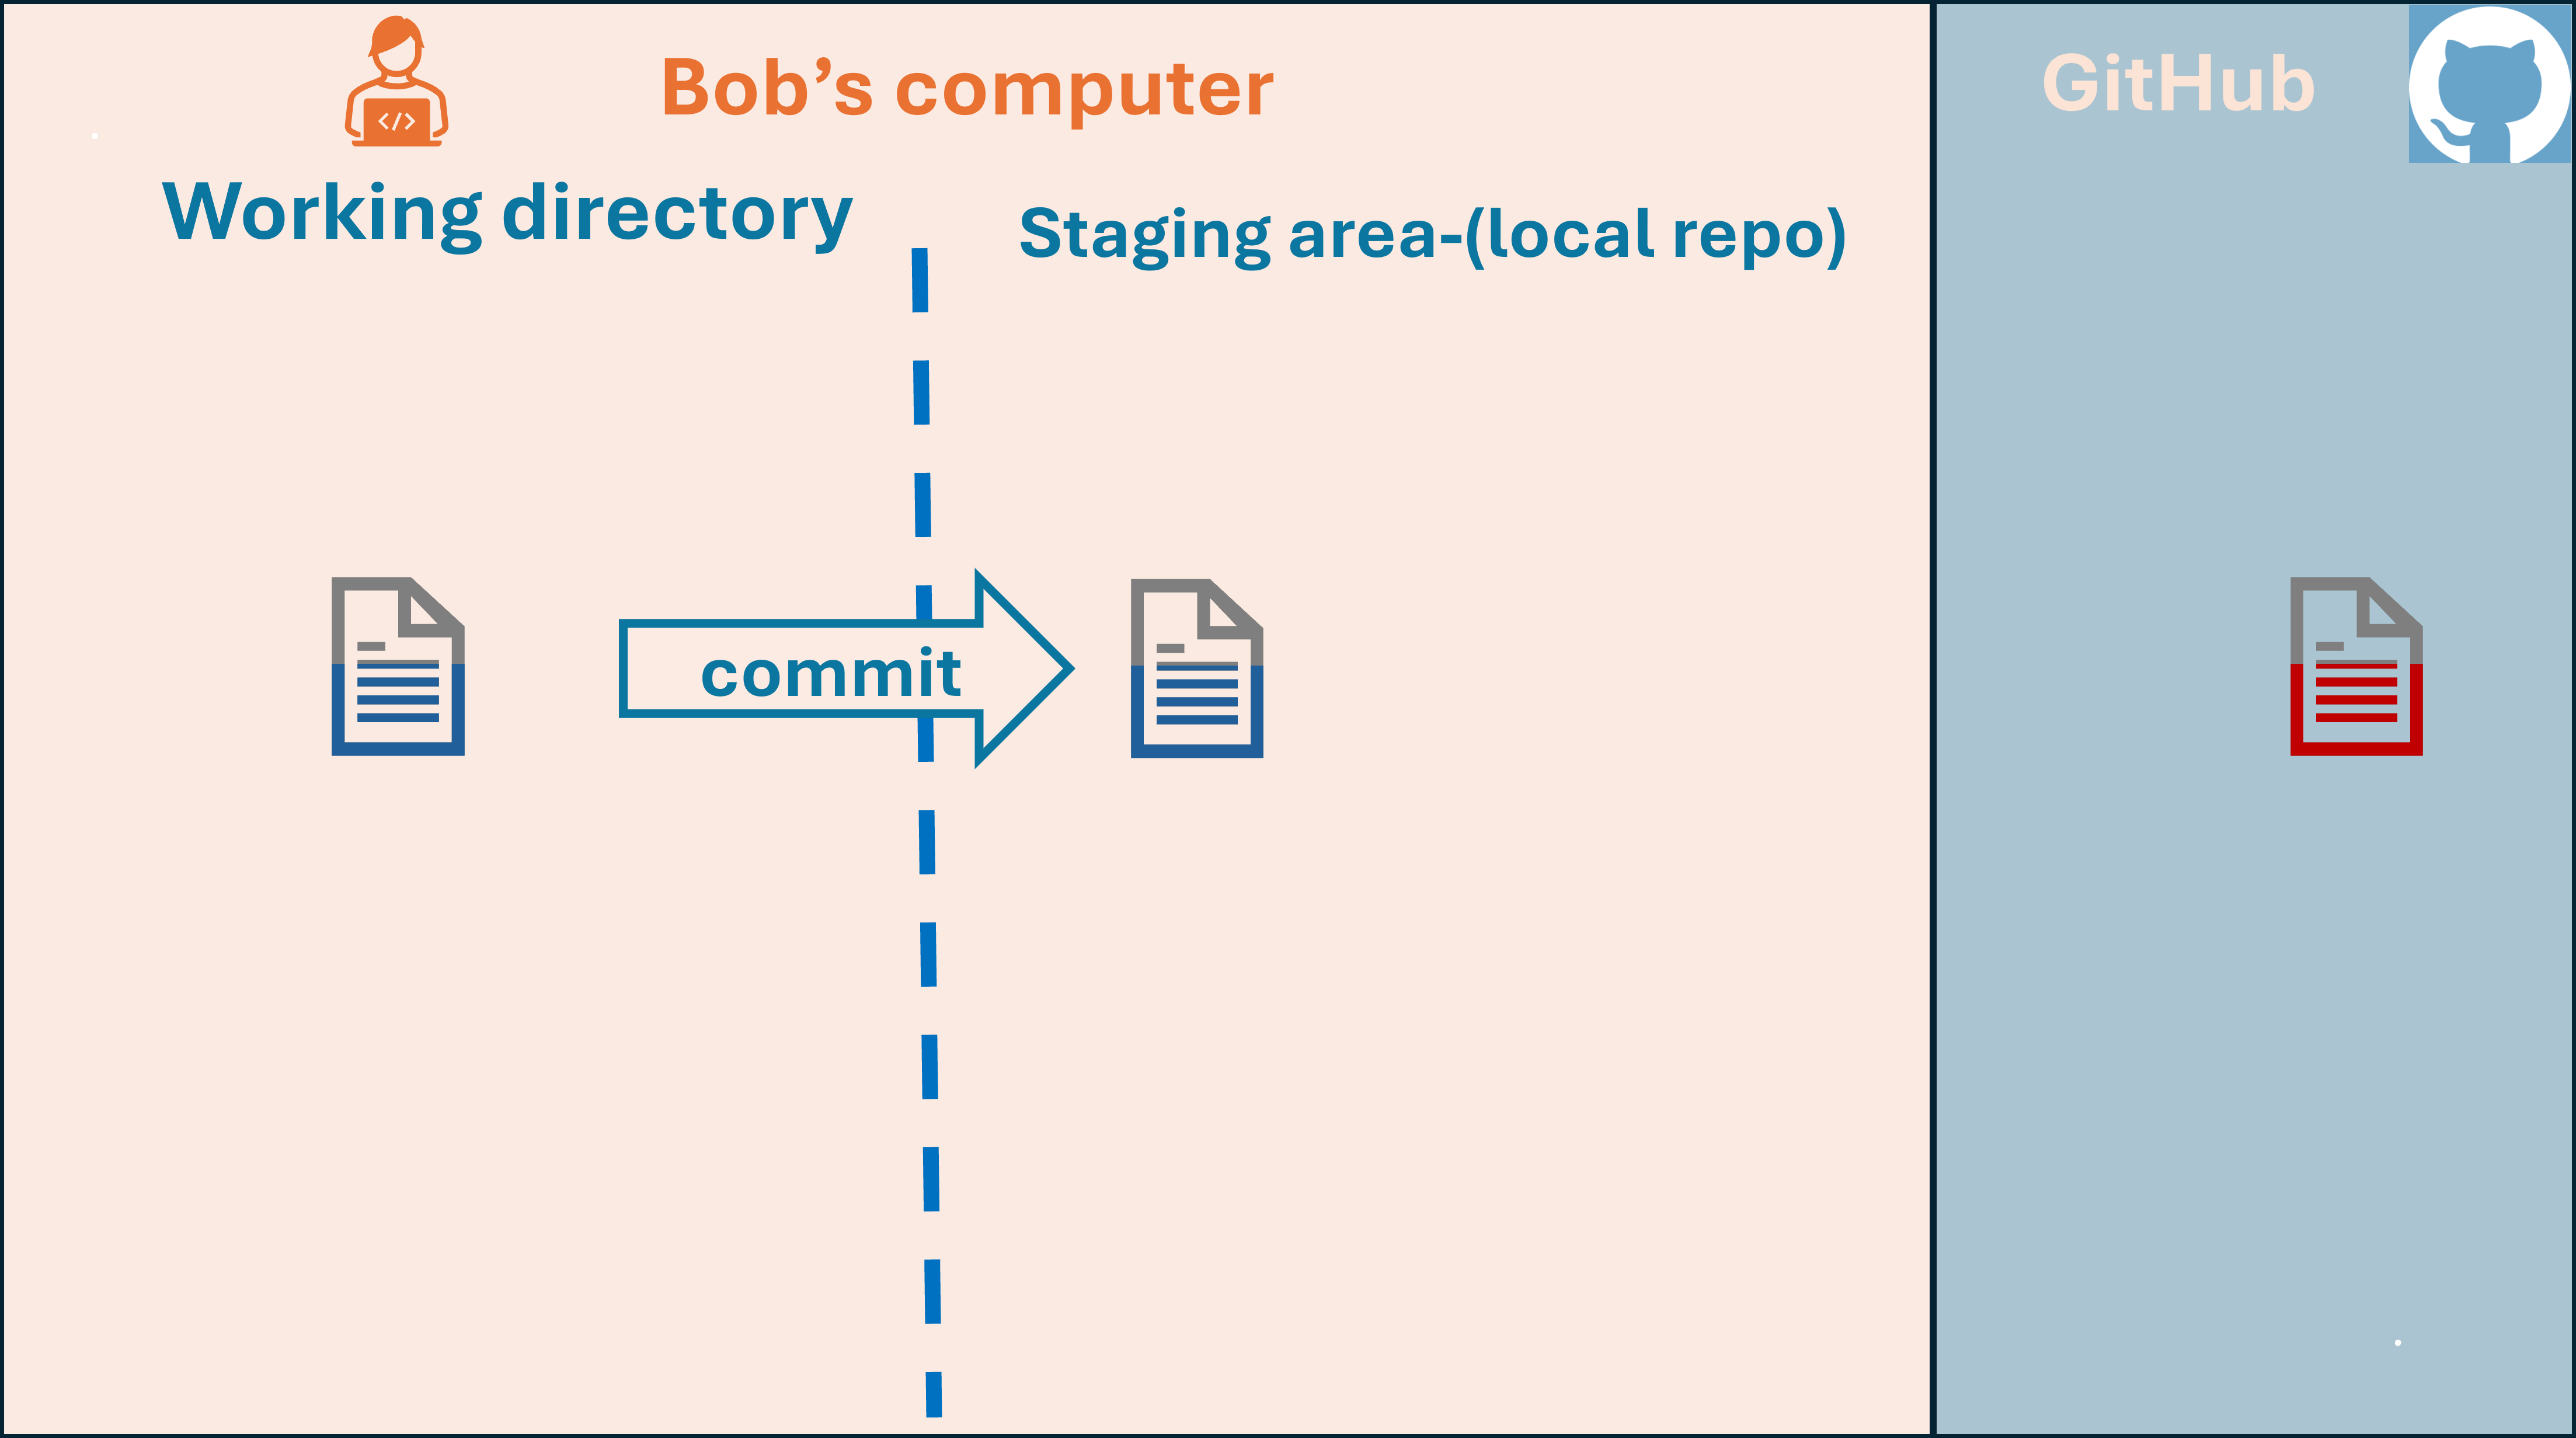
\includegraphics[width=1.0\textwidth]{GitComplex6N.png} \\ }
\only<7>{\includegraphics[width=1.0\textwidth]{GitComplex7N.png} \\ }
\only<8>{\includegraphics[width=1.0\textwidth]{GitComplex8N.png} \\ }
\only<9>{\includegraphics[width=1.0\textwidth]{GitComplex9N.png} \\ }
\only<10>{\includegraphics[width=1.0\textwidth]{GitComplex10N.png} \\ }
\end{itemize}
\end{frame}

\begin{frame}
\begin{center}
\Large{ \color{brique}{Tea Break}}
\vspace{0.5cm}

\includegraphics[height=0.5\textwidth]{tea-cup-cuppa-food-drink.jpg}
\end{center}
\end{frame}


\section{Principles- part 3}

\begin{frame}[<+->]
   \frametitle{RAP principles 3 :  \\Good (coding) Practices}
   \pause
    \begin{itemize}[<+->]
     \item Good coding practices
     \item[$\hookrightarrow$] Write for humans, not for machines
     \item Testing
     \item Peer-review
     \item \href{https://sergegoussev.github.io/ESCAP_RAP_class/docs/teaching_materials/sept_18/sept_18_session.html\#principle-6-good-coding-practices}{\emph{Exercise part 3:}}  Coding, documenting, testing. (15 minutes)
    \end{itemize}
\end{frame}


\section{Takeway}

\begin{frame}
\frametitle{Towards a full RAP}

 \begin{itemize}[<+->]
        \item In short,\\
        \begin{center} \textbf{RAP}\\ =\\ Reproducible documents\\+ \\ Version Control \\+ \\ Automation \\  \end{center}
        \item Each of these notion require training
        \item New tools, new challenges, new problems...
        \item[$\hookrightarrow$]  Requires time, patience and training
        \item Doing RAP is like doing sports: You'll not becoming a champion immediately! 
        \item Practicing regularly helps progressing though,  starting from Bronze level
    \end{itemize}
\end{frame}



\end{document}




\section{Version Control}

\begin{frame} % Cover slide
\frametitle{Version Control keeps tracks of your work}
Tracking three \textbf{W} questions:
\begin{columns}[t]
 \begin{column}{0.5\textwidth}
 \begin{itemize}[<+->]
 \item[] \textcolor{siap}{\textbf{W}}hat changes?
 \item[] \textcolor{siap}{\textbf{W}}ho made the changes?
 \item[] \textcolor{siap}{\textbf{W}}hen were the changes made?
 \end{itemize}
 \end{column}
  \begin{column}{0.5\textwidth}
    \begin{center}
    \begin{itemize}
        \only<1-4>{ \includegraphics[width=0.95\textwidth]{FileHistory.PNG} \\  }
       \only<1-4>{\hfill  \textcolor{gris}{\tiny{Source: \href{https://the-turing-way.netlify.app/reproducible-research/vcs.html}{The Turing Way project}}}}
    \end{itemize}
    \end{center}
  \end{column}
\end{columns}
\end{frame}

\begin{frame}
\frametitle{Git  \& GitHub}
\begin{center}
    Git \& GitHub are different tools
\end{center}
\begin{columns}[t]
 \begin{column}{0.5\textwidth}
 \begin{itemize}[<+->]
  \item[]{\begin{center}
              \includegraphics[width=0.2\textwidth]{git_logo.jpg} \\
             \end{center} }
        \item Git is a software
        \item Git needs to be installed
        \item Git works mostly in command mode
        \item Git is complex and unfriendly!

    \end{itemize}
 \end{column}
 \begin{column}{0.5\textwidth}
 \begin{itemize}[<+->]
  \item[]{\begin{center}
              \includegraphics[width=0.4\textwidth]{GitHub-logo.png} \\
             \end{center} }
        \item GitHub is a platform
        \item GitHub needs an account
        \item GitHub can only be accessed remotely
        \item GitHub is (more) friendly
    \end{itemize}
 \end{column}
\end{columns}
\end{frame}


\section{Git \& GitHub}

\begin{frame}
\frametitle{Setup}

What you'll need to do...
\begin{columns}[t]
 \begin{column}{0.8\textwidth}

 \begin{itemize}[<+->]
        \item Download Git
        \item Install Git on your computer
        \item[$\hookrightarrow$]  Depends on your OS
        \item Create a  GitHub account
        \item Link Git with GitHub account
        \item Link VStudio with Git
        \item[$\hookrightarrow$] May need IT support
        \item[$\hookrightarrow$] Many tutorials exist
    \end{itemize}
 \end{column}
  \begin{column}{0.2\textwidth}
    \begin{center}
    \begin{itemize}
        \only<1-8>{ \includegraphics[width=0.6\textwidth]{git_logo.jpg} \\  }
        \only<4-8>{\vspace{0.1 cm} \includegraphics[width=0.95\textwidth]{GitHub-logo.png}  \\  }
        \only<6-8>{ \vspace{0.1cm}  \includegraphics[width=0.6\textwidth]{VisualStudio-Logo.png} \\  }
    \end{itemize}
    \end{center}
  \end{column}
\end{columns}
\end{frame}



\begin{frame}{Version Control in a Nutshell }
Version control system:
\begin{columns}[t]
\begin{column}{0.6\textwidth}
\begin{itemize}[<+->]
    \item Allows to travel back in time
    \item Keeps track of all changes
    \item Allows to "undo" at any point
    \item Allows reviewing stages of development
    \item Allow collaborating on projects
    \item Backups your work
  \end{itemize}
 \end{column}
  \begin{column}{0.4\textwidth}
    \begin{center}
    \begin{itemize}
        \only<1-6>{\includegraphics[width=0.8\textwidth]{github-mark.png} }
        \only<1-6>{ \textcolor{gris}{\tiny{ \href{https://www.c-sharpcorner.com/article/git-for-absolute-beginners-with-command-line-interface/}{GitHub logo}}}}
    \end{itemize}
    \end{center}
  \end{column}
\end{columns}
\end{frame}

\section{Takeway}

\begin{frame}
\frametitle{Towards a full RAP}

 \begin{itemize}[<+->]
        \item In short,\\
         \begin{center} \textbf{RAP}\\ =\\ Reproducible documents\\+ \\ Version Control \\+ \\ Automation \end{center}
        \item Each of these notion require training
        \item New tools, new challenges, new problems...
        \item[$\hookrightarrow$]  Requires time, patience and training
        \item Git is powerful, but complex
        \item[$\hookrightarrow$] It works with \includegraphics[width=6ex]{VisualStudio-Logo.png}
        \item Automation is hard
        \item Building a RAP is a collective process \\
        \includegraphics[width=0.5\textwidth]{DecolonisingKnowledge.jpg}
    \end{itemize}
\end{frame}



\section{Resources}
\begin{frame}{Useful resources}
  \begin{itemize}
   \item  \href{https://github.com/sergegoussev/ESCAP_RAP_class/tree/main}{This course website} (created by Serge Goussev)
   \item \href{https://github.com/Vanuatu-National-Statistics-Office/vnso-RAP-marketStats-materials}{Vanuatu Bureau of Statistics implementation of RAP}
   \item \href{https://www.unsiap.or.jp/on_line/2024/RAP/flyer-RAP-Self-paced.pdf}{SIAP's (free) online RAP course}
    \item The UK government RAP \href{https://ukgovdatascience.github.io/rap-website/index.html}{website}.
    \item UK best practice \href{https://gss.civilservice.gov.uk/policy-store/quality-statistics-in-government/\#reproducible-analytical-pipelines-rap-}{documentation}.
    \item A free RAP \href{https://www.udemy.com/course/reproducible-analytical-pipelines/}{course} to teach you all you need to know.
    \item How the Data Science Campus sets its coding \href{https://datasciencecampus.github.io/coding-standards/}{standards}.
    \item A new open-source \href{https://the-turing-way.netlify.com}{book} from the Alan Turing institute setting out how to do reproducible data science.
  \end{itemize}
\end{frame}




\end{document}


